% Class, Font size, Paper shape, isDraft
\documentclass[a4paper, 10pt, final]{article} % Document class: [draft] sets pdf output to draft quality, [<number>pt] sets font size in range of 10-12pt
\usepackage{import} % Import other latex documents (here for 3d plot variables definition)
\usepackage{shellesc}

%% Todo
\usepackage[obeyFinal]{easy-todo}

%% Margins
\usepackage[margin=2.5cm]{geometry} % Margins: \newgeometry{<options>} can set margins individually

%% Language, Fonts, Encoding
\usepackage[russian]{babel}                         % Input encoding language
\usepackage{fontspec}                               % XeTeX font settings
\defaultfontfeatures{Ligatures=TeX, Numbers=Lining} % OTF font features for all fonts
\setmainfont{Linux Libertine O}                     % Set serif (main) font
\setsansfont{Linux Biolinum O}                      % Set sans serif font
\setmonofont{Inconsolata}                           % Set monospace font
\usepackage{amsmath, amssymb}                       % Math support
\newcommand{\mathbff}[1]{$\boldsymbol{#1}$}

%% Paragraph, Line spacings
\setlength{\parindent}{2em}
\setlength{\parskip}{1.5ex}
\renewcommand{\baselinestretch}{1.0}

%% Text alignment
\usepackage{ragged2e} % Text alignment correction (\Centering, \RaggedRight, \RaggedLeft, \justifying)

%% Headers & Footers
\usepackage{fancyhdr}                                                        % Headers conFiguration package
\pagestyle{fancy}                                                            % {fancy}: keyword for custom headers and footers
\fancyhead[L]{\textbf{LAM: Проектирование аналоговых фильтров}}              % Header settings
\fancyhead[R]{2021/2022}
\fancyfoot[R,L]{}                                                            % Footer settings
\fancyfoot[C]{\thepage}
\renewcommand{\headrulewidth}{0.5pt}                                         % Header line thickness
\renewcommand{\footrulewidth}{1pt}                                           % Footer line thickness
\usepackage[stable, marginal, bottom, para]{footmisc}                        % Footers fix: [stable] prevents footers in titles, [bottom] deletes space left on the bottom,[marginal] puts footers near margin, [para] puts multiple footers on one line
\renewcommand{\footnoterule}{\noindent\smash{\rule[3pt]{\textwidth}{0.5pt}}} % Footnote line

%% Bibliography, References
\usepackage[style=apa, sorting=nty]{biblatex}             % Bibliography: [style=apa] won't mix references with footer naming, [sorting=nty] "Name, Title, Year" is most sensible to use in terms of searchability
\usepackage{csquotes}                                     % Babel & quotes behaviour fix
\addbibresource{LAM_Design_dei_filtri_analogici.bib}      % File with bibliograpy sorces information
\newcommand{\parenciteit}[2]{\textit{\parencite[#1]{#2}}} % Italic parencite (citation in parenthesis)
\usepackage{hyperref}                                     % Clickable references: [hidelinks]
\hypersetup{
    colorlinks=true,
    linkcolor=blue,
    filecolor=blue,
    citecolor=blue,
    urlcolor=cyan,
}
%% Biblates Hyperref fix
\DeclareFieldFormat{citehyperref}{%
  \DeclareFieldAlias{bibhyperref}{noformat}% Avoid nested links
  \bibhyperref{#1}}

\DeclareFieldFormat{textcitehyperref}{%
  \DeclareFieldAlias{bibhyperref}{noformat}% Avoid nested links
  \bibhyperref{%
    #1%
    \ifbool{cbx:parens}
      {\bibcloseparen\global\boolfalse{cbx:parens}}
      {}}}

\savebibmacro{cite}
\savebibmacro{textcite}

\renewbibmacro*{cite}{%
  \printtext[citehyperref]{%
    \restorebibmacro{cite}%
    \usebibmacro{cite}}}

\renewbibmacro*{textcite}{%
  \ifboolexpr{
    ( not test {\iffieldundef{prenote}} and
      test {\ifnumequal{\value{citecount}}{1}} )
    or
    ( not test {\iffieldundef{postnote}} and
      test {\ifnumequal{\value{citecount}}{\value{citetotal}}} )
  }
    {\DeclareFieldAlias{textcitehyperref}{noformat}}
    {}%
  \printtext[textcitehyperref]{%
    \restorebibmacro{textcite}%
    \usebibmacro{textcite}}}

%% Graphics
\usepackage{graphicx}                                    % Support for images
\usepackage{ifluatex}
% \ifluatex
%   \usepackage{pdftexcmds}
%   \makeatletter
%   \let\pdfstrcmp\pdf@strcmp
%   \let\pdffilemoddate\pdf@filemoddate
%   \makeatother
% \fi
\usepackage{pdfpages}                             % Support for pdf insertion
\usepackage{tikz}                                        % Support for vector graphics
\usetikzlibrary{
    calc,                                                % Support for coordinate operations in tikz
    patterns,                                            %
    positioning,                                         %
    shapes.geometric,                                    %
    shapes.arrows,                                       %
    decorations.pathmorphing,                            %
    matrix,                                              %
    chains,                                              %
    scopes,                                              %
    arrows,                                              %
    fit,                                                 %
    shadows,                                             %
    backgrounds                                          %
}
% \usepackage{pgfkeys}
\usepackage{float}                                       % Support for floats fix
\usepackage[section]{placeins}                           % Support for FloatBarrier
\usepackage{caption}                                     % Support for cpations inside tikz
\usepackage{subcaption}                                  % Support for captions inside subfigures
\usepackage[nooldvoltagedirection, european]{circuitikz} % Support for electric circuit diagrams
\def \circuitsscale{0.6}                                 % Default value for circuit scale in this document

%% Enumerations
\usepackage{enumitem} % Support for different symbols in enumeration blocks

%% Circuit macros
\newcommand{\opampPMCenter}[1]{($(#1.+)!0.5!(#1.-)$) coordinate(opampPMCenter-PM) ($(#1.center) - (opampPMCenter-PM)$)  coordinate(opampPMCenter)} % Opamp center macro

%% Plots
\usepackage{pgfplots}
\usepackage{pgf}
\pgfplotsset{compat=1.17}
\usepgfplotslibrary{patchplots}
\usepgfplotslibrary{colormaps}
\usetikzlibrary{pgfplots.colorbrewer}

%% Styles & common definitions
\tikzset{>=stealth}
\tikzset{font_size/.style={font=\footnotesize}}
\tikzstyle{block}=[
    align=center,
    draw,
    minimum height=1.5em,
    fill=white,
    drop shadow={fill=gray}
]

\pgfplotsset{
    compat=1.9,
    clip=false,
    scaled y ticks=false,
    scaled x ticks=false,
    axis_style_default/.style={
        legend pos=outer north east,
        legend cell align={left},
        axis line style={->},
        legend style={font=\footnotesize},
        label style={font=\footnotesize},
        tick label style={font=\footnotesize},
        xlabel style={
            at={(ticklabel* cs:1)},
            anchor=west,
            font=\footnotesize,
        },
        ylabel style={
            at={(ticklabel* cs:1)},
            anchor=south,
            font=\footnotesize,
        },
        samples=500,
    },
    axis_style_default_data/.style={
        legend pos=outer north east,
        legend cell align={left},
        axis line style={->},
        legend style={font=\footnotesize},
        label style={font=\footnotesize},
        tick label style={font=\footnotesize},
        xlabel style={
            at={(ticklabel* cs:1)},
            anchor=west,
            font=\footnotesize,
        },
        ylabel style={
            at={(ticklabel* cs:1)},
            anchor=south,
            font=\footnotesize,
        },
    },
    x_axis_style_pi/.style={
        trig format plots=rad,
        scaled x ticks={real:\PI},
        xtick scale label code/.code={},
        xtick distance=pi/#1,
        xticklabel={
            \pgfmathparse{round(100*\tick)/100}
            \ifdim \pgfmathresult pt = 1pt
                \strut$\pi$
            \else\ifdim \pgfmathresult pt = -1pt
                \strut$-\pi$
            \else
                \pgfmathifisint{\pgfmathresult}{%
                    \strut$\pgfmathprintnumber[int detect]{\pgfmathresult}\pi$%
                }
                {
                    % \pi in numerator
                    \strut$\pgfmathprintnumber{\pgfmathresult}\pi$%
                    % % \pi in the numerator of the frac
                    % \pgfmathparse{\pgfmathresult*#1}%
                    % \strut$\frac{\pgfmathprintnumber[int detect]{\pgfmathresult}\pi}{#1}$%
                }
            \fi\fi
        },
        % set number plotting to frac style
        xticklabel style={
            /pgf/number format/.cd,
            frac,
            frac whole=false,
            % % if you prefer to have the same denominator value everywhere
            % frac denom=#1,
        },
    }
}
\usepackage{listings}

% define precision of \pi
\pgfmathsetmacro{\PI}{pi}

\pgfplotsset{
  colormap/twilight/.style={colormap={twilight}{[1pt]
  rgb(0pt)=(0.8857501584075443, 0.8500092494306783, 0.8879736506427196);
  rgb(25pt)=(0.38407269378943537, 0.46139018782416635, 0.7309466543290268);
  rgb(50pt)=(0.18488035509396164, 0.07942573027972388, 0.21307651648984993);
  rgb(75pt)=(0.6980608153581771, 0.3382897632604862, 0.3220747885521809);
  rgb(100pt)=(0.8857115512284565, 0.8500218611585632, 0.8857253899008712);
}},
  colormap/twilight_shifted/.style={colormap={twilight_shifted}{[1pt]
rgb(0pt)=(0.18739228342697645, 0.07710209689958833, 0.21618875376309582);
rgb(25pt)=(0.38407269378943537, 0.46139018782416635, 0.7309466543290268);
rgb(50pt)=(0.8857115512284565, 0.8500218611585632, 0.8857253899008712);
rgb(75pt)=(0.6980608153581771, 0.3382897632604862, 0.3220747885521809);
rgb(100pt)=(0.18488035509396164, 0.07942573027972388, 0.21307651648984993);
}}}

\newcommand{\InvisibleBorder}{
    (current bounding box.south west) ++($(-\fboxsep, -\fboxsep)-(0.5,0.5)$) coordinate (ll)
    (current bounding box.north east) ++($(\fboxsep, \fboxsep)+(0.5,0.5)$) coordinate (ur)
}

\captionsetup{
    format=plain,
    labelfont=bf,
    font=small,
    justification=centering
}

% Externalise optimisation
\usetikzlibrary{external}
\usepgfplotslibrary{external}
\tikzexternalize
\tikzsetexternalprefix{cache/}
% [2026 devbox rebuild] Original 2022 build externalised figures with lualatex
% (see cache/*-figure*.log). Modern pgf auto-picks xelatex here, which chokes on
% \directlua 3D-plot code — pin the system call to lualatex explicitly.
\tikzset{external/system call={lualatex \tikzexternalcheckshellescape -shell-escape -halt-on-error -interaction=nonstopmode -jobname "\image" "\texsource"}}
% [2026 devbox rebuild] tikz's includegraphics-optimization breaks pdfpages'
% \AM@currentdocname@fix in the externalisation children (TeX Live 2025):
\tikzset{external/optimize=false}

%%%%%%%%%%%%%%
%% Document %%
%%%%%%%%%%%%%%

\begin{document}
    \begin{titlepage}
        \begin{center}
            \vspace*{\stretch{2}}
            \huge\textbf Проектирование аналоговых фильтров

            \vspace*{1ex}
            \Large{\texttt{Evgeny Kartashov}}

            \vspace*{3ex}
            \large{\textbf{Liceo cantonale di Lugano 1}}

            \large{\textbf{Учебный год 2021/2022}}
            
            \vspace*{\stretch{3}}
            
            \begin{figure}[H]
                \centering
                \begin{minipage}[H]{.45\linewidth}
                    \centering
                    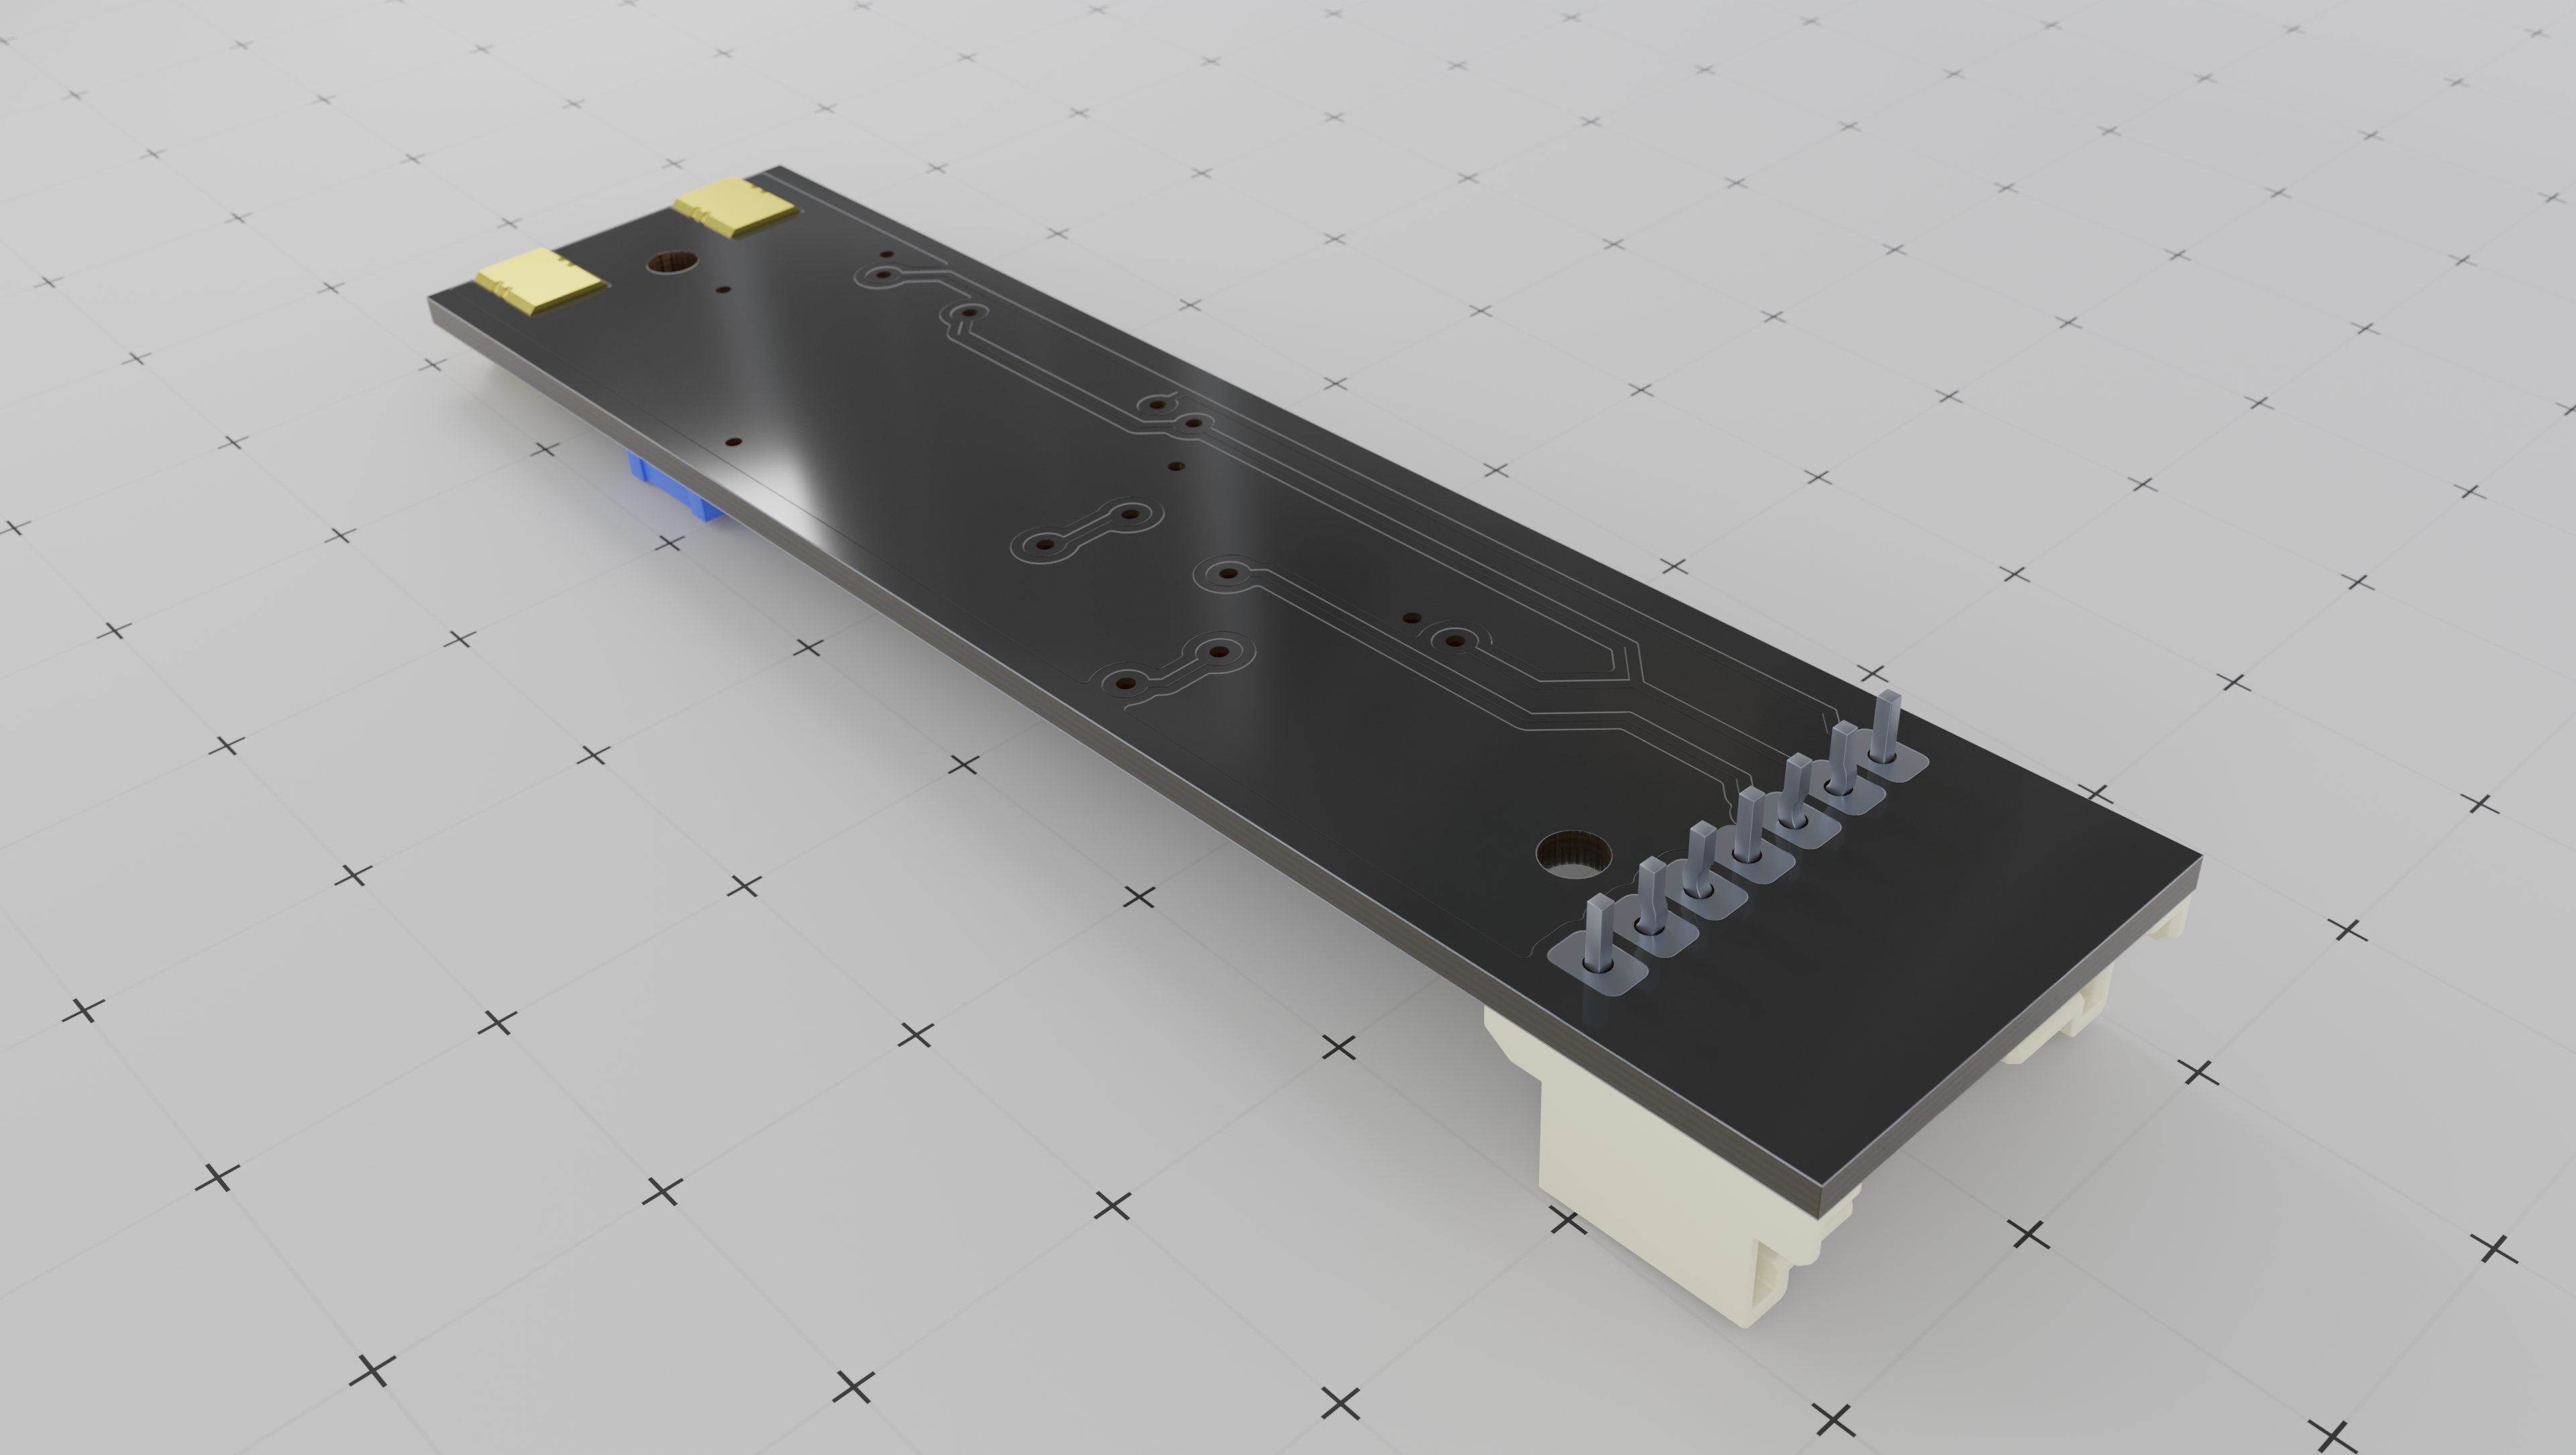
\includegraphics[width=\linewidth]{media/Render3.png}
                \end{minipage}
                \hspace{.04\linewidth}
                \begin{minipage}[H]{.45\linewidth}
                    \centering
                    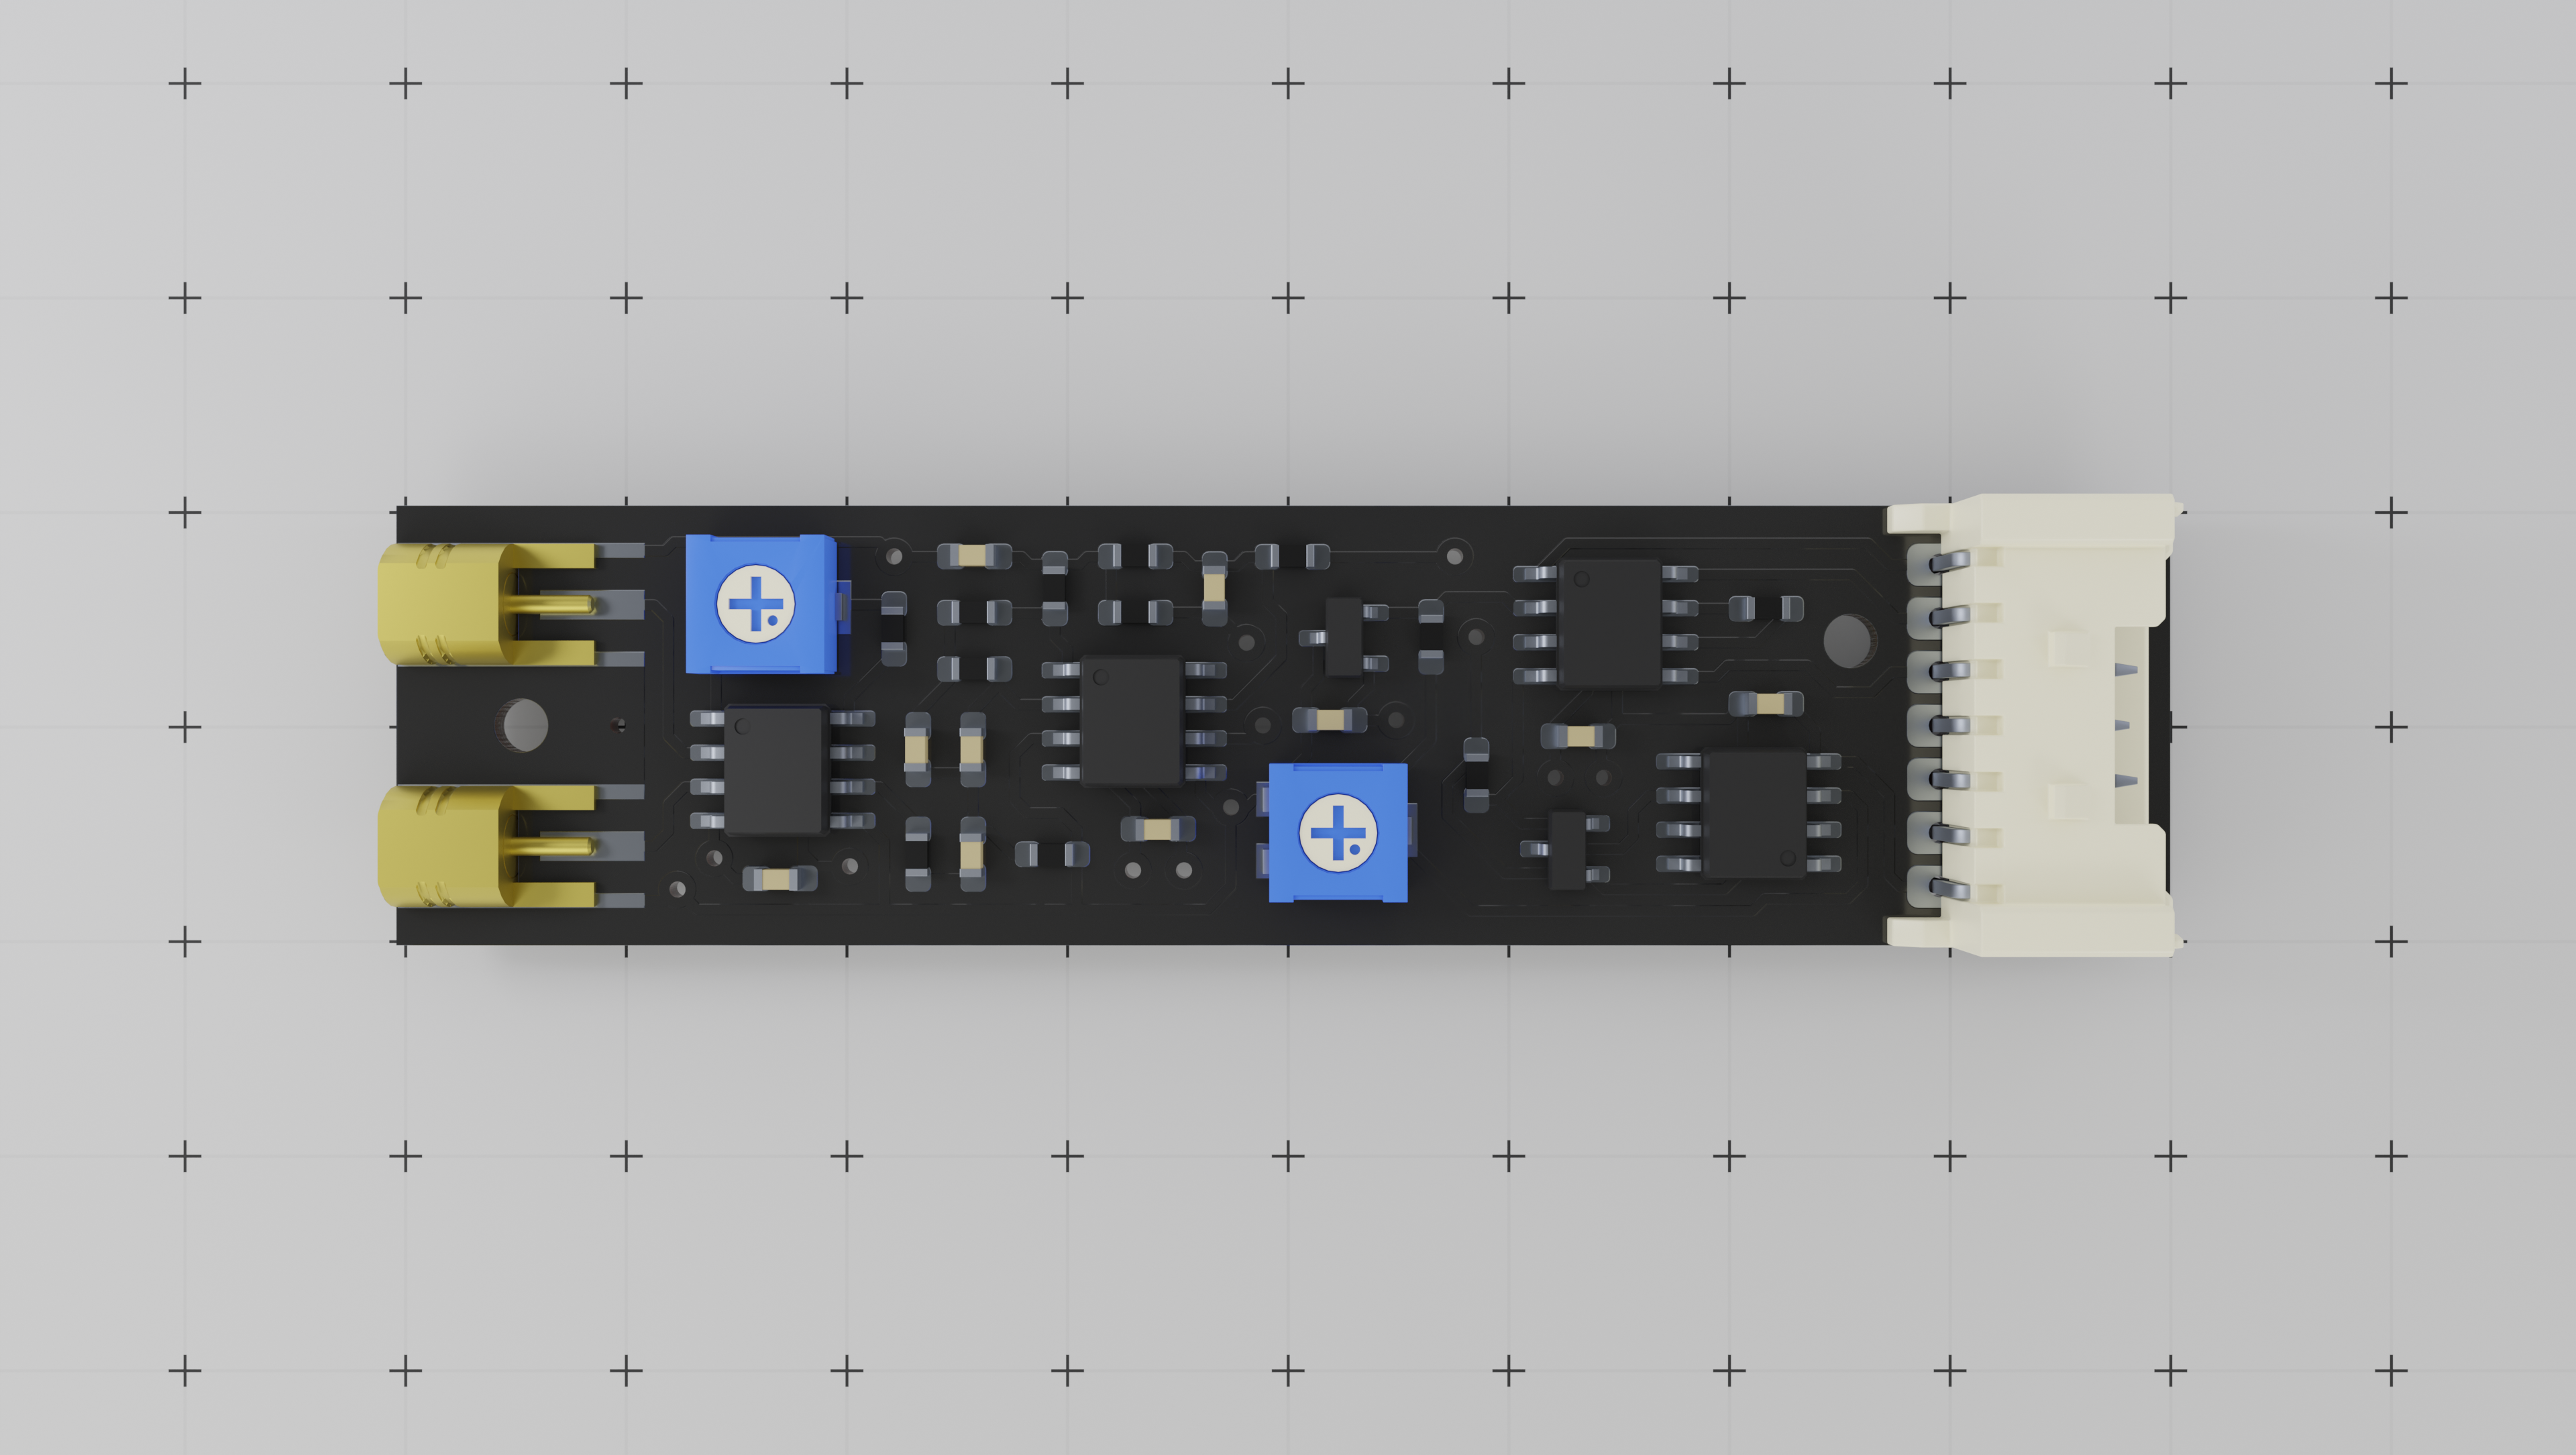
\includegraphics[width=\linewidth]{media/Render2.png}
                \end{minipage}
                \\
                \vspace*{.04\linewidth}
                \begin{minipage}[H]{.95\linewidth}
                    \centering
                    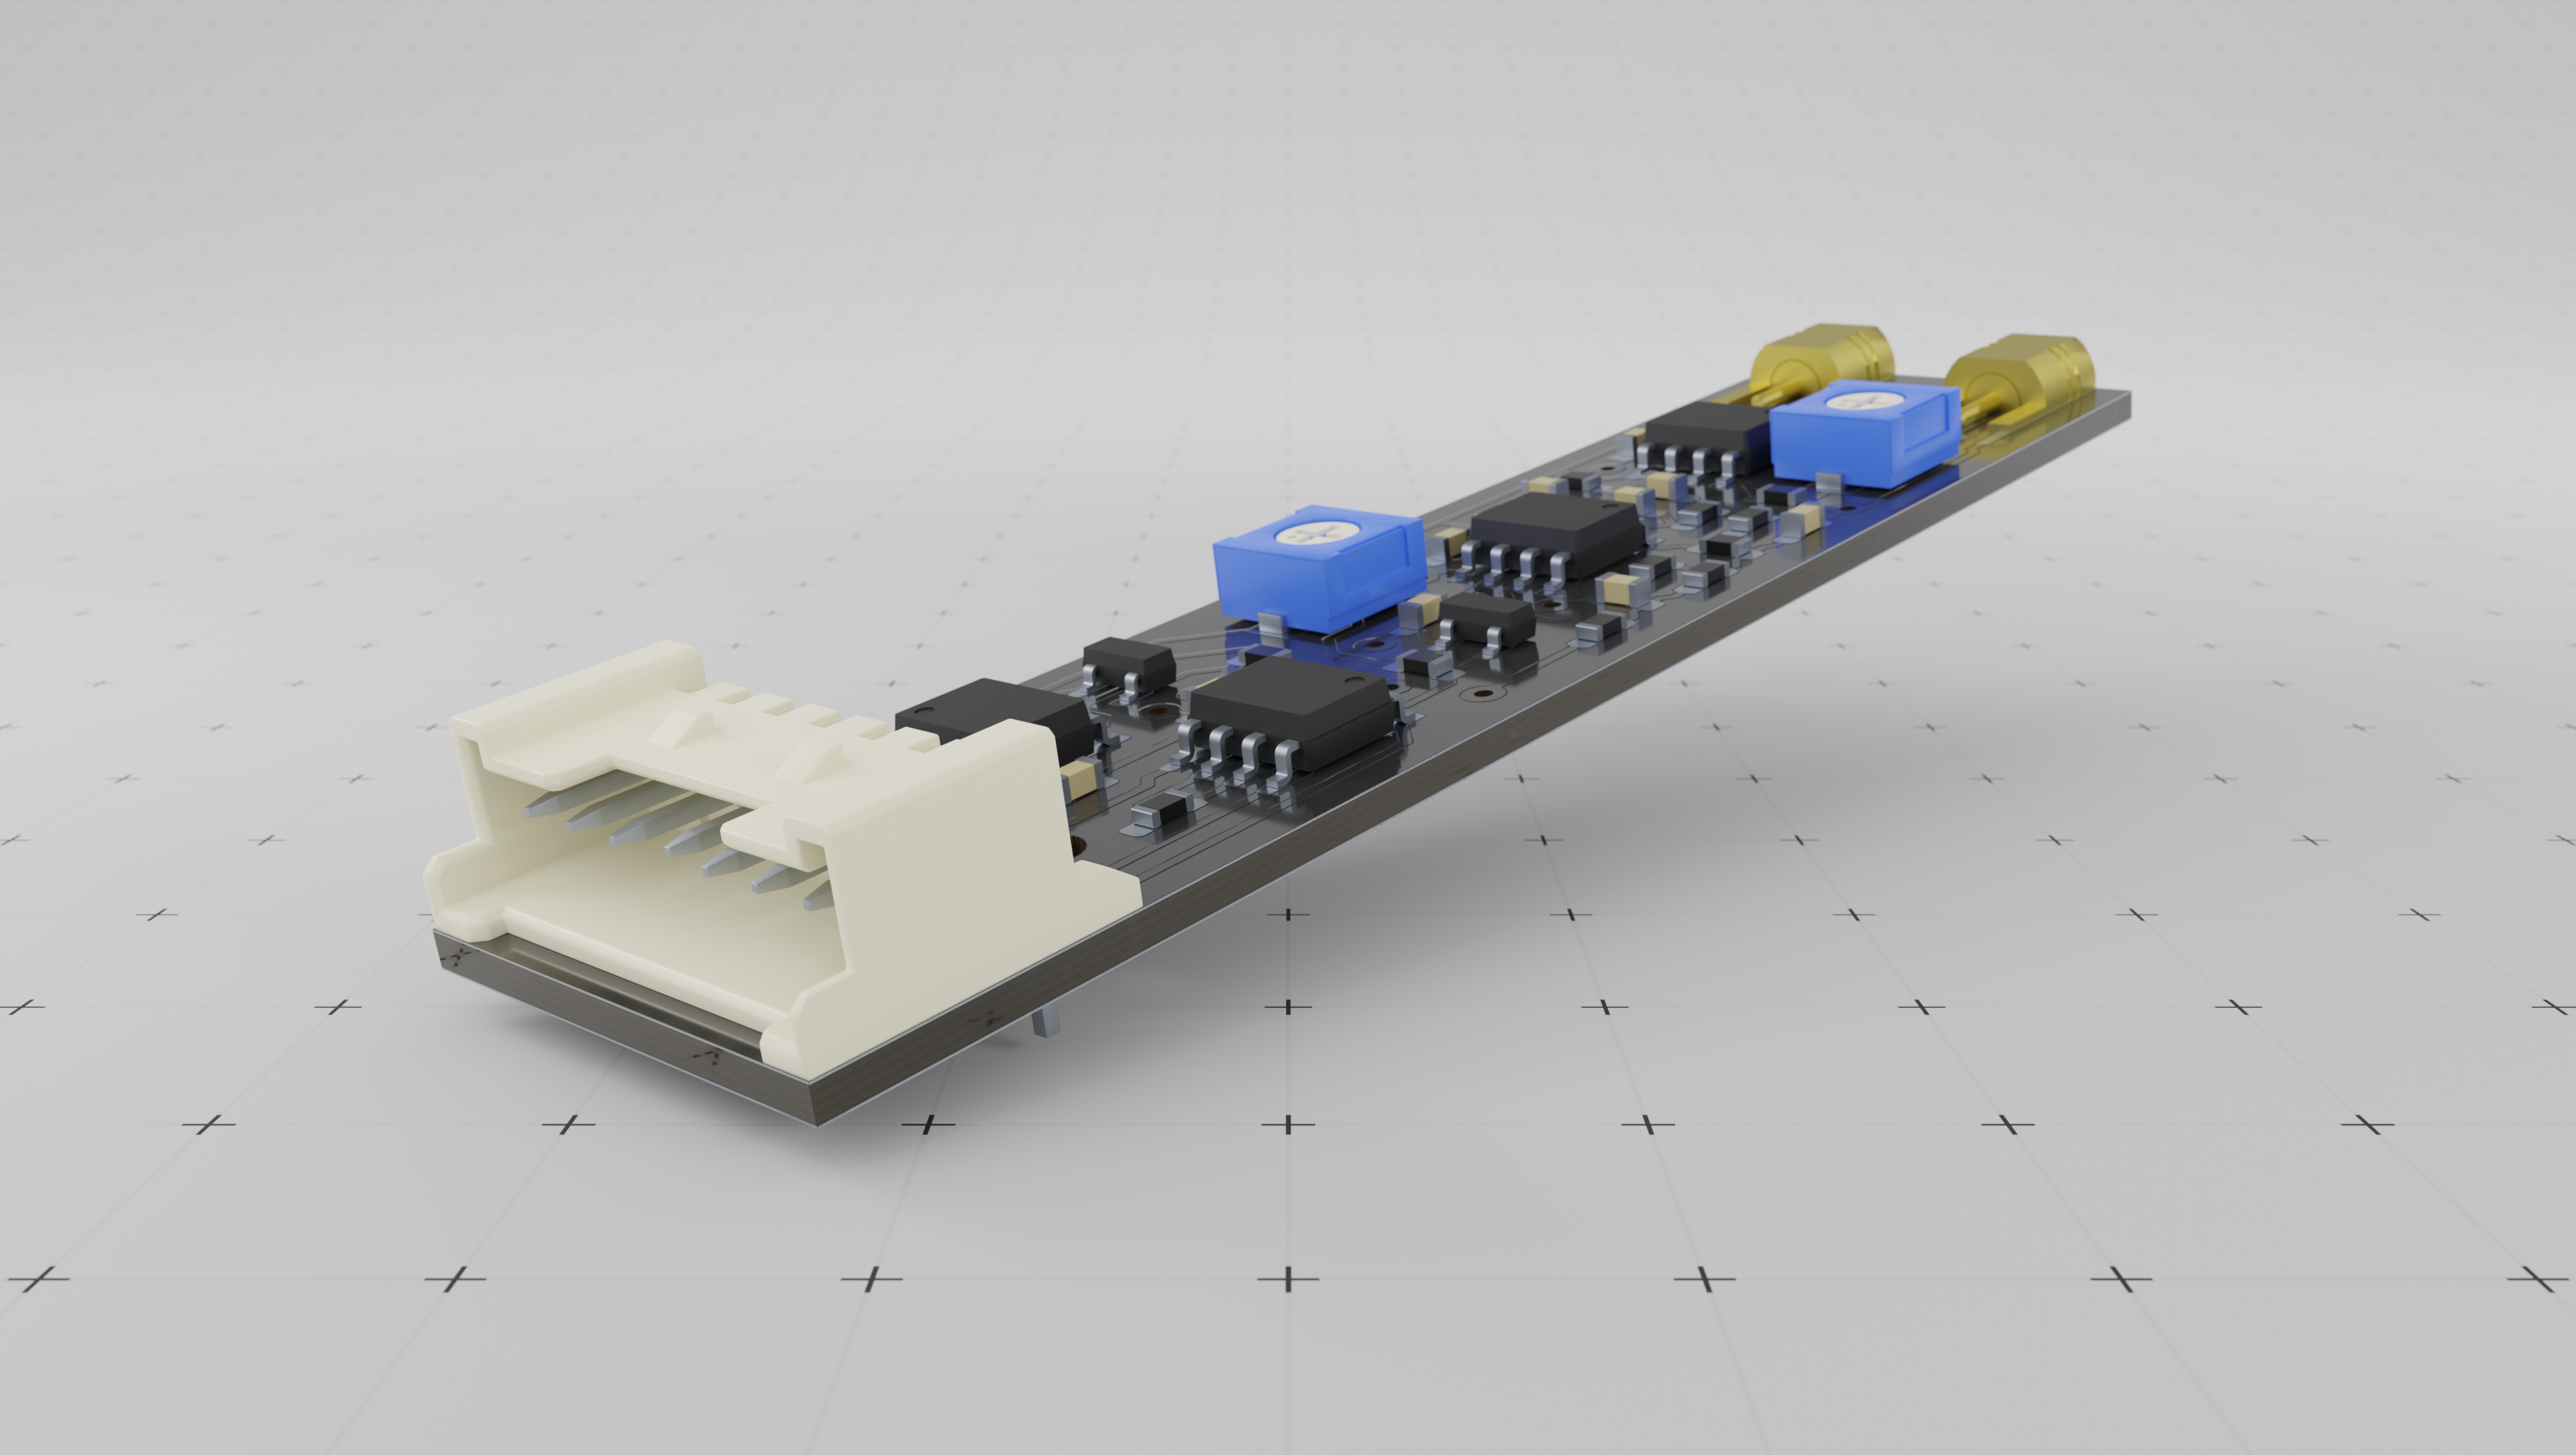
\includegraphics[width=\linewidth]{media/Render1.png}
                \end{minipage}
            \end{figure}
            
            \vspace*{\stretch{2}}
        \end{center}
    \end{titlepage}

    \clearpage
    % \listoftodos
    % \clearpage

    \section*{Аннотация}
    \par Аналоговые фильтры --- неизбежный\footnote{Невозможность их исключения обсуждается в разделе \ref{sec:ProjectDesignAbstractModel}, последний список из 6 пунктов}\todo{Проверить количество пунктов} и незаменимый компонент технологий XXI века: они входят во внутреннее устройство электрических приборов, начиная со смартфонов и заканчивая научными измерительными приборами.
    Из источников, которые можно найти в интернете, очень сложно извлечь информацию, необходимую для того, чтобы выполнить практичное и эффективное проектирование аналоговых фильтров.
    Именно поэтому среди увлечённых электротехникой людей много тех, кто считает, что проектировать фильтры легко, то есть достаточно пары формул, которые, конечно, дают некоторую информацию, но то, что они оставляют без внимания, восполняется интуицией человека.
    Я же, напротив, считаю, что эта тема должна быть совершенно ясна всем, кто считает себя увлечённым электротехникой.
    Главная тема этого документа --- проектирование аналоговых фильтров не только на теоретическом, но и на практическом уровне: в конце документа представлена настоящая плата, которая способна улавливать чрезвычайно слабые сигналы с поверхности кожи, усиливать их и передавать в виде данных на компьютер.
    Излагаемая теория обширна, но не чрезмерно, --- ровно настолько, чтобы понять, как работают фильтры, как их проектировать и затем изготавливать.
    \clearpage
    \tableofcontents

    \clearpage
    \section{Введение}\label{sec:Intro}
    \subsection{Мотивация}\label{sec:IntroMotivation}
    Ещё до начала выпускной работы \emph{maturit\`{a}} я всё сильнее ощущал отсутствие личного транспортного средства и заинтересовался решением этой проблемы.
    Учитывая бюджет, желаемое качество и конкретные характеристики: портативность, небольшие размеры и вес, ремонтопригодность и возможность заменить транспортное средство, я решил сделать электрический скейтборд.
    
    Вопросом, на котором я задержался больше всего, был пульт управления, поскольку скейтбордом должен управлять человек, который на нём едет.
    Изучив вопрос, я обнаружил, что в настоящее время\footnote{В 2021 году} на технологическом рынке электрические скейтборды оснащаются довольно простыми пультами с кнопками и каким-либо их аналоговым вариантом\footnote{С более чем двумя состояниями}, позволяющим дозировать мощность, с которой включаются двигатели.
    Поэтому я решил\footnote{Факторы, повлиявшие на выбор, будут объяснены в разделе \ref{sec:IntroReader}} придерживаться гораздо менее стандартной идеи, которая к тому же кажется мне либо новой, либо редко используемой: концепции жестового управления в сочетании с транспортным средством.
    
    По удачному совпадению дат, во время разработки проекта мне также нужно было написать выпускную работу \emph{maturit\`{a}} на тему робототехники, то есть также физико-математическую, которая предполагала создание роботизированного прототипа на основе собственных исследований. Разумеется, я постарался сохранить текущий проект, который, к сожалению, взятый целиком, оказался слишком обширным для выпускной работы \emph{maturit\`{a}}. Тогда, руководствуясь привлекательностью создания устройства, которое не занимало бы руку во время использования\footnote{При падении или любой непредвиденной ситуации желательно, чтобы руки были сразу свободны; кроме того, я считаю, что это повышает удобство}, и собственным мнением об оригинальности идеи, я решил представить небольшую его часть: аналоговую часть электромиографического датчика\footnote{Термины и причины выбора будут пояснены в разделе \ref{sec:IntroReader}}; далее\footnote{Раздел \ref{sec:IntroMotivation}} станет ясно, что речь идёт главным образом о фильтре.
    
    \subsection{Цель работы}\label{sec:IntroAim}
    \noindent Цель этой выпускной работы \emph{maturit\`{a}}:
    \begin{enumerate}[label=\emph{(\roman*)}]
        \item Познакомить читателя с понятием фильтров и с тем, как они работают с точки зрения сигналов
        \item Дать относящуюся к ним терминологию
        \item Ответить на вопросы, возникшие в ходе разработки проекта
        \item Обратить внимание на соображения, которые нужно учитывать при теоретическом и практическом проектировании
        \item Построить прототип в качестве проверки концепции
    \end{enumerate}
    Кроме того, многие знания, изложенные в выпускной работе \emph{maturit\`{a}}, применимы и в других областях, например: математическая модель фильтров полностью справедлива и для цифровых фильтров, а практические детали\footnote{Как в разделе \ref{sec:BuildingHardware}} \todo{добавить часть про блокировочные конденсаторы, индуктивность, сплошной слой земли и скин-эффект} проектирования схем применимы почти к любому другому типу прецизионных схем.
    
    Содержание также включает ход рассуждений\footnote{Подробное рассуждение о причинах, ведущих к использованию фильтра, и о последствиях его использования}, предшествующий процессу разработки фильтра, который помогает встроить фильтр в проект, вместо того чтобы рассматривать концепцию изолированно и оставлять без ответа ключевые вопросы, которые могут возникнуть при работе над следующим проектом.
    
    \subsection{Организация работы}\label{sec:IntroOrganization}
    Особенности проекта, такие как использованные методы управления проектами\footnote{Термин и обозначаемая им характеристика будут рассмотрены в разделе \ref{sec:ProjectCharacteristics}} и размер проекта по сравнению с той его частью, которая представлена в выпускной работе \emph{maturit\`{a}}, диктуют правила организации проекта, которые я рассматриваю в этом разделе.
    Если бы процесс, определяемый методами и сложностью проекта, документировался в хронологическом порядке, текст получился бы слишком объёмным, плохо соответствующим теме выпускной работы \emph{maturit\`{a}} и зачастую запутанным.
    
    \begin{samepage}
        \noindent Схема, которой я следую при документировании всей выпускной работы \emph{maturit\`{a}}, чтобы решить проблемы организации, следующая:
        \begin{enumerate}[label=\emph{(\roman*)}]
            \item Теория \& практика
            \item Характеристики
            \item Проектирование
        \end{enumerate}
    \end{samepage}
    Стоит отметить, что эта трёхчастная схема не пытается придать всей выпускной работе \emph{maturit\`{a}} форму «\emph{Введение}», «\emph{Основная часть}», «\emph{Заключение}», а стремится упорядочить содержание по концептуальным группам, чтобы затем построить на них связное изложение с последовательным и логичным ходом, при этом не отрицая наличия основной схемы как только что упомянутого стандарта «де-факто»\footnote{Принятого в качестве формального стандарта из-за его очевидности для большого числа людей}.
    
    Часть \emph{Теория \& практика} служит для того, чтобы дать читателю информацию, необходимую для понимания тем, затрагиваемых в последующих частях.
    Часть \emph{Характеристики} служит для того, чтобы понять, какими характеристиками должен обладать или обладает объект и какие из них влияют на следующую часть и на последующие иерархически подчинённые объекты.
    Часть \emph{Проектирование} --- это часть, где посредством рассуждений обосновываются и утверждаются сделанные решения; они всегда тесно связаны с предыдущими частями того же объекта и с предшествующими объектами.
    Разумеется, части \emph{Характеристики} и \emph{Проектирование} содержат теоретические и практические элементы, но когда рассматриваемая информация становится слишком обширной, чтобы описать её в одном разделе, она выносится в отдельный раздел \emph{Теория \& практика}, который ставится перед ними.
    
    \begin{samepage}
        \noindent Пример может быть таким:
        \begin{enumerate}[label=\emph{(\roman*)}]
            \item Раздел \ref{sec:IntroFiltersSignals} $\Rightarrow$ \emph{Теория \& практика}
            \item Раздел \ref{sec:ProjectCharacteristics} $\Rightarrow$ \emph{Характеристики}
            \item Раздел \ref{sec:ProjectDesign} $\Rightarrow$ \emph{Проектирование}
        \end{enumerate}
    \end{samepage}

    \subsection{Введение в работу}\label{sec:IntroReader}
    Чтобы ввести читателя в выпускную работу \emph{maturit\`{a}}, в этом разделе я объясняю основные понятия, необходимые для того, чтобы следить за изложением, и в сжатом виде привожу рассуждения, относящиеся к той части работы, которая была выполнена до этапа разработки датчиков.

    Из теории и практики я предпочитаю начать с теоретической части, чтобы показать читателю простую модель, которую можно развивать, усложнять и совершенствовать по ходу чтения.
    
    Если обобщить максимально, то решаемая задача --- это передача информации на небольшое расстояние.
    Я посчитал, что единственным логичным направлением для поиска решения является электроника --- благодаря возможности создавать компактные устройства и передавать информацию по радиоканалу\footnote{Радиочастоты (RF)}, который по определению является проявлением электромагнетизма\footcite[«Поле» (электромагнитное) «можно рассматривать как сочетание электрического и магнитного полей»]{Electromagnetism:Wiki} \footcite[«Электричество связано с магнетизмом, поскольку оба являются частью явления электромагнетизма»]{Electricity:Wiki}.
    Затем я применил метод абстракции с помощью аналогии с \emph{Input/Output} \footcite[]{IO:Wiki}.
    Он состоит в том, чтобы понять, какими возможными «\emph{Output}\footnote{Выходы информации}» обладает объект, от которого нужно собирать информацию, что они вызывают с физической точки зрения, и, наконец, выбрать явления, чтобы затем преобразовать их в обратную связь\footnote{Ответный сигнал}, в нашем случае электрическую.
    Если объект --- человек, то выражать информацию позволяют только \emph{движение} человека или частей его тела и производство \emph{звуков} \footnote{Голос, хлопки в ладоши, свист и т.\,д.}.
    Я выбрал передачу информации с помощью движений именно для того, чтобы не влиять на звуки, чтобы избежать возможных помех\footnote{Они возможны и при движениях, но объективно реже, поскольку звуки распространяются по воздуху} и потому, что нет особой необходимости в чрезмерно сложном словаре\footnote{Сказано применительно к голосовому управлению}.
    Движения могут быть любыми, например перенос веса тела вперёд или назад относительно транспортного средства, однако этому способу не хватило детальности управления, и он мешал пользоваться транспортным средством\footnote{Нужно идеальное чувство равновесия, чтобы сохранять контроль в такие моменты, как разгон и торможение}.
    \clearpage  
    \noindent Поскольку ни одно другое движение не казалось достаточно удобным, последней оставшейся возможностью была рука, которая оказалась очень эффективной благодаря детальности управления и гибкости.
    Применив во второй раз только что упомянутый метод\footnote{Метод, использующий аналогию с Input/Output},
    я получил разные идеи возможных вариантов «\emph{Output}» объекта\footnote{Анализ Input/Output для руки} \emph{(обозначены цифрами)} и идеи решений для их использования \emph{(обозначены буквами)}:
    \begin{enumerate}[label=\emph{(\arabic*)}]
        \item Изменение положения пальцев и кисти
            \begin{enumerate}[label=\emph{(\alph*)}]
                \item Перчатка с поворотными энкодерами\footnote{Датчик угла поворота} \footnote{Существуют разные типы поворотных энкодеров: контактные, оптические, на эффекте Холла (магнитные)}\emph{(рисунок \ref{fig:IdeaEncoderGlove})} с пружинами и нитями или с датчиками изгиба\footnote{Flex sensors} \footnote{Они меняют сопротивление в зависимости от того, насколько согнуты}\emph{(рисунок \ref{fig:IdeaFlexGlove})}
                \item Браслет с электромагнитным радаром, таким как чип «Soli»\footcite[]{GoogleATAP:Wiki} \emph{(рисунок \ref{fig:IdeaRadarGlove})}
                \item MEMS-датчики\footnote{Сочетание гироскопа, акселерометра и иногда датчиков магнитного поля Земли для точного определения положения в пространстве} на каждом пальце и на кисти \emph{(рисунок \ref{fig:IdeaMEMSGlove})}
            \end{enumerate}
        \item Изменение диаметра мышц при сокращении
        \item Изменение электрического поля в нерве из-за переносимого им сигнала, а следовательно, и в мышце из-за её сокращения \label{ItemDeltaChoice}
            \begin{enumerate}[label=\emph{(\alph*)}]
                \item Игольчатые электроды \emph{(рисунок \ref{fig:IdeaNeedleEMGBand})}, поверхностные контактные или поверхностные ёмкостные электроды \emph{(рисунок \ref{fig:IdeaSurfaceEMGBand})}, на которые действует изменение электрического заряда из-за электромагнитных полей, создаваемых мышцей и/или нервом \label{ItemEMG}
            \end{enumerate}
    \end{enumerate}

    \begin{figure}[H]
        \centering
        \begin{minipage}[H]{.32\linewidth}
            \centering
            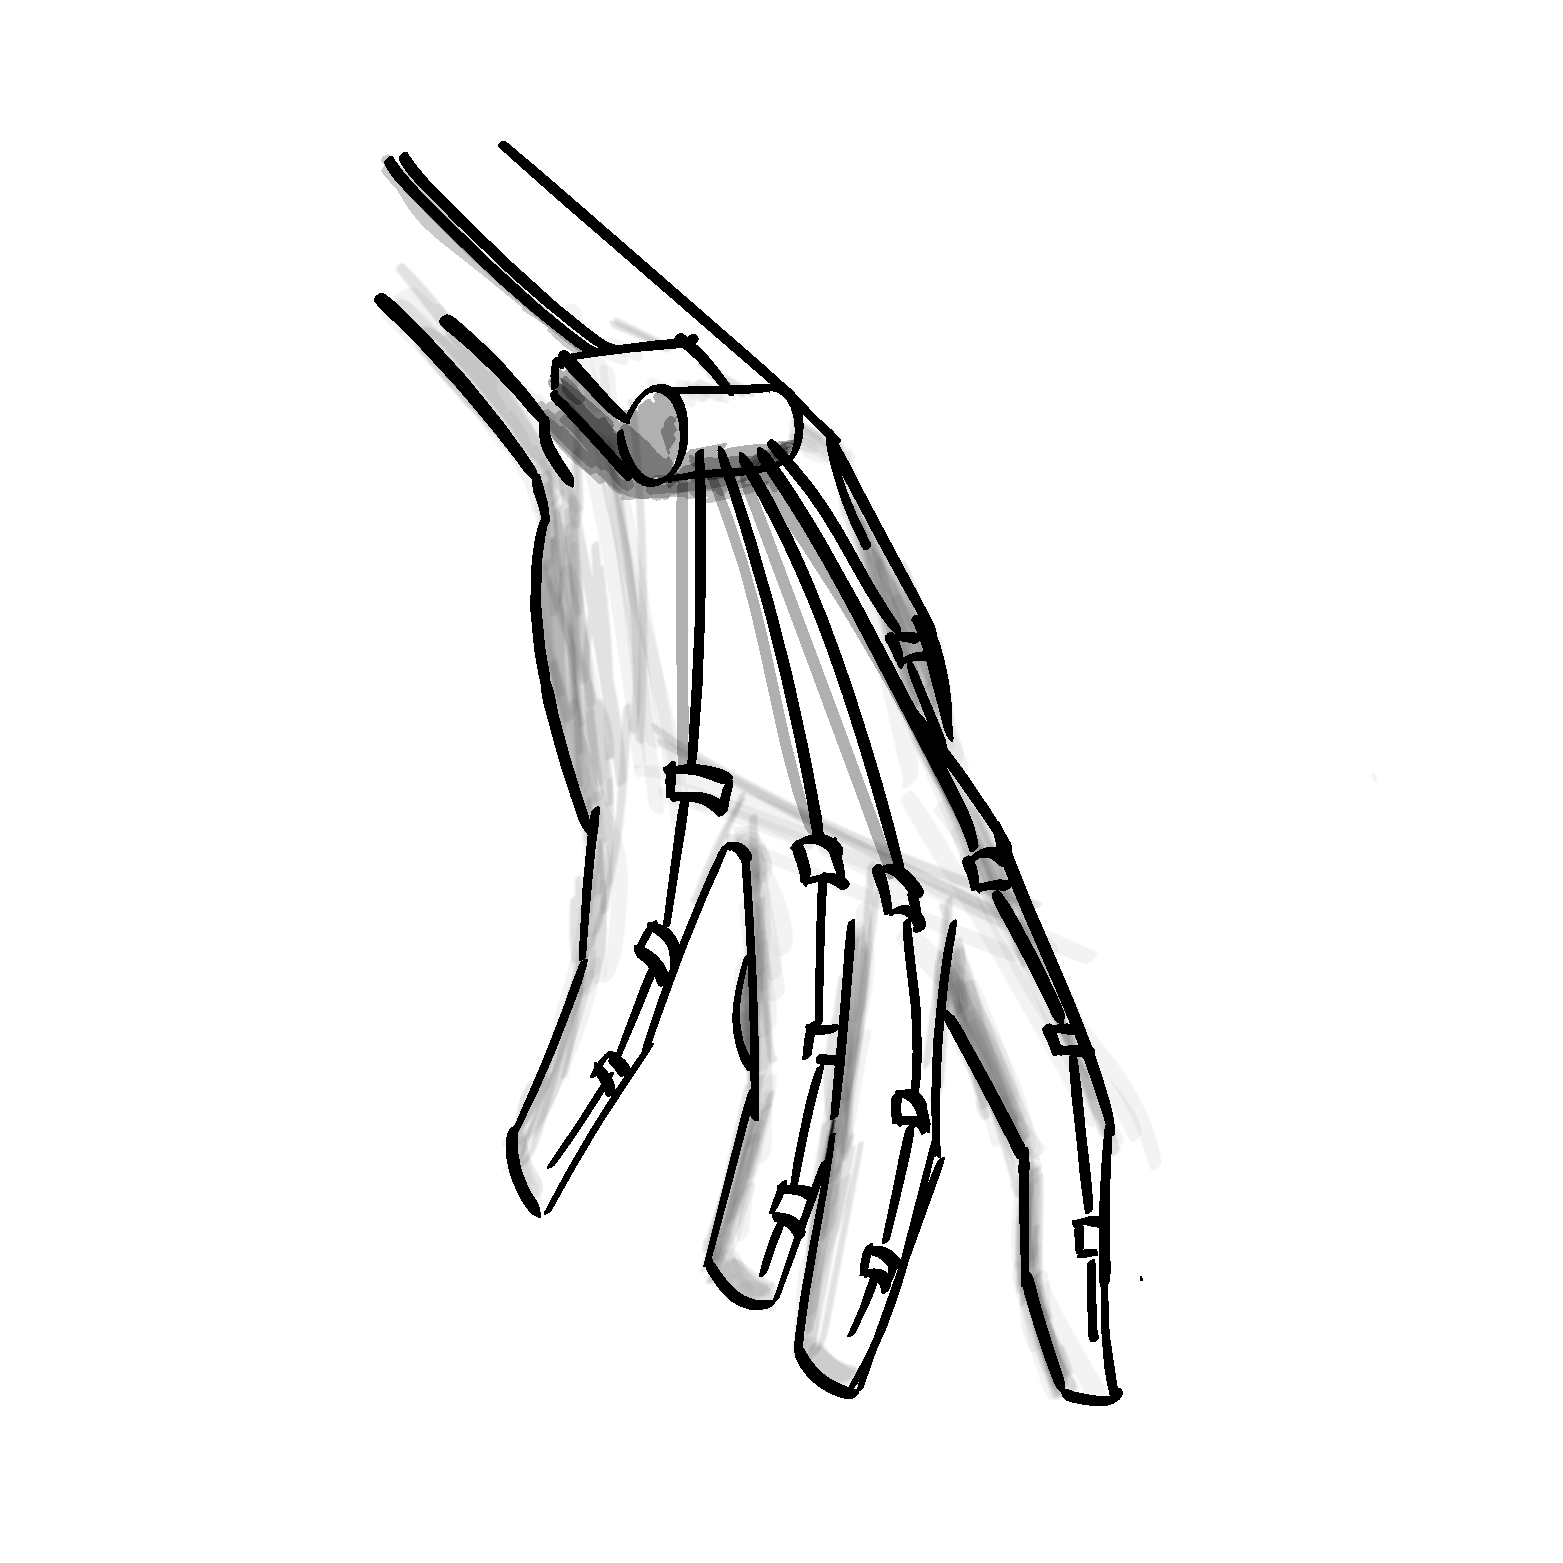
\includegraphics[page=1, width=\linewidth]{media/Ideasheet1.pdf}
            \subcaption{}\label{fig:IdeaEncoderGlove}
        \end{minipage}
        \begin{minipage}[H]{.32\linewidth}
            \centering
            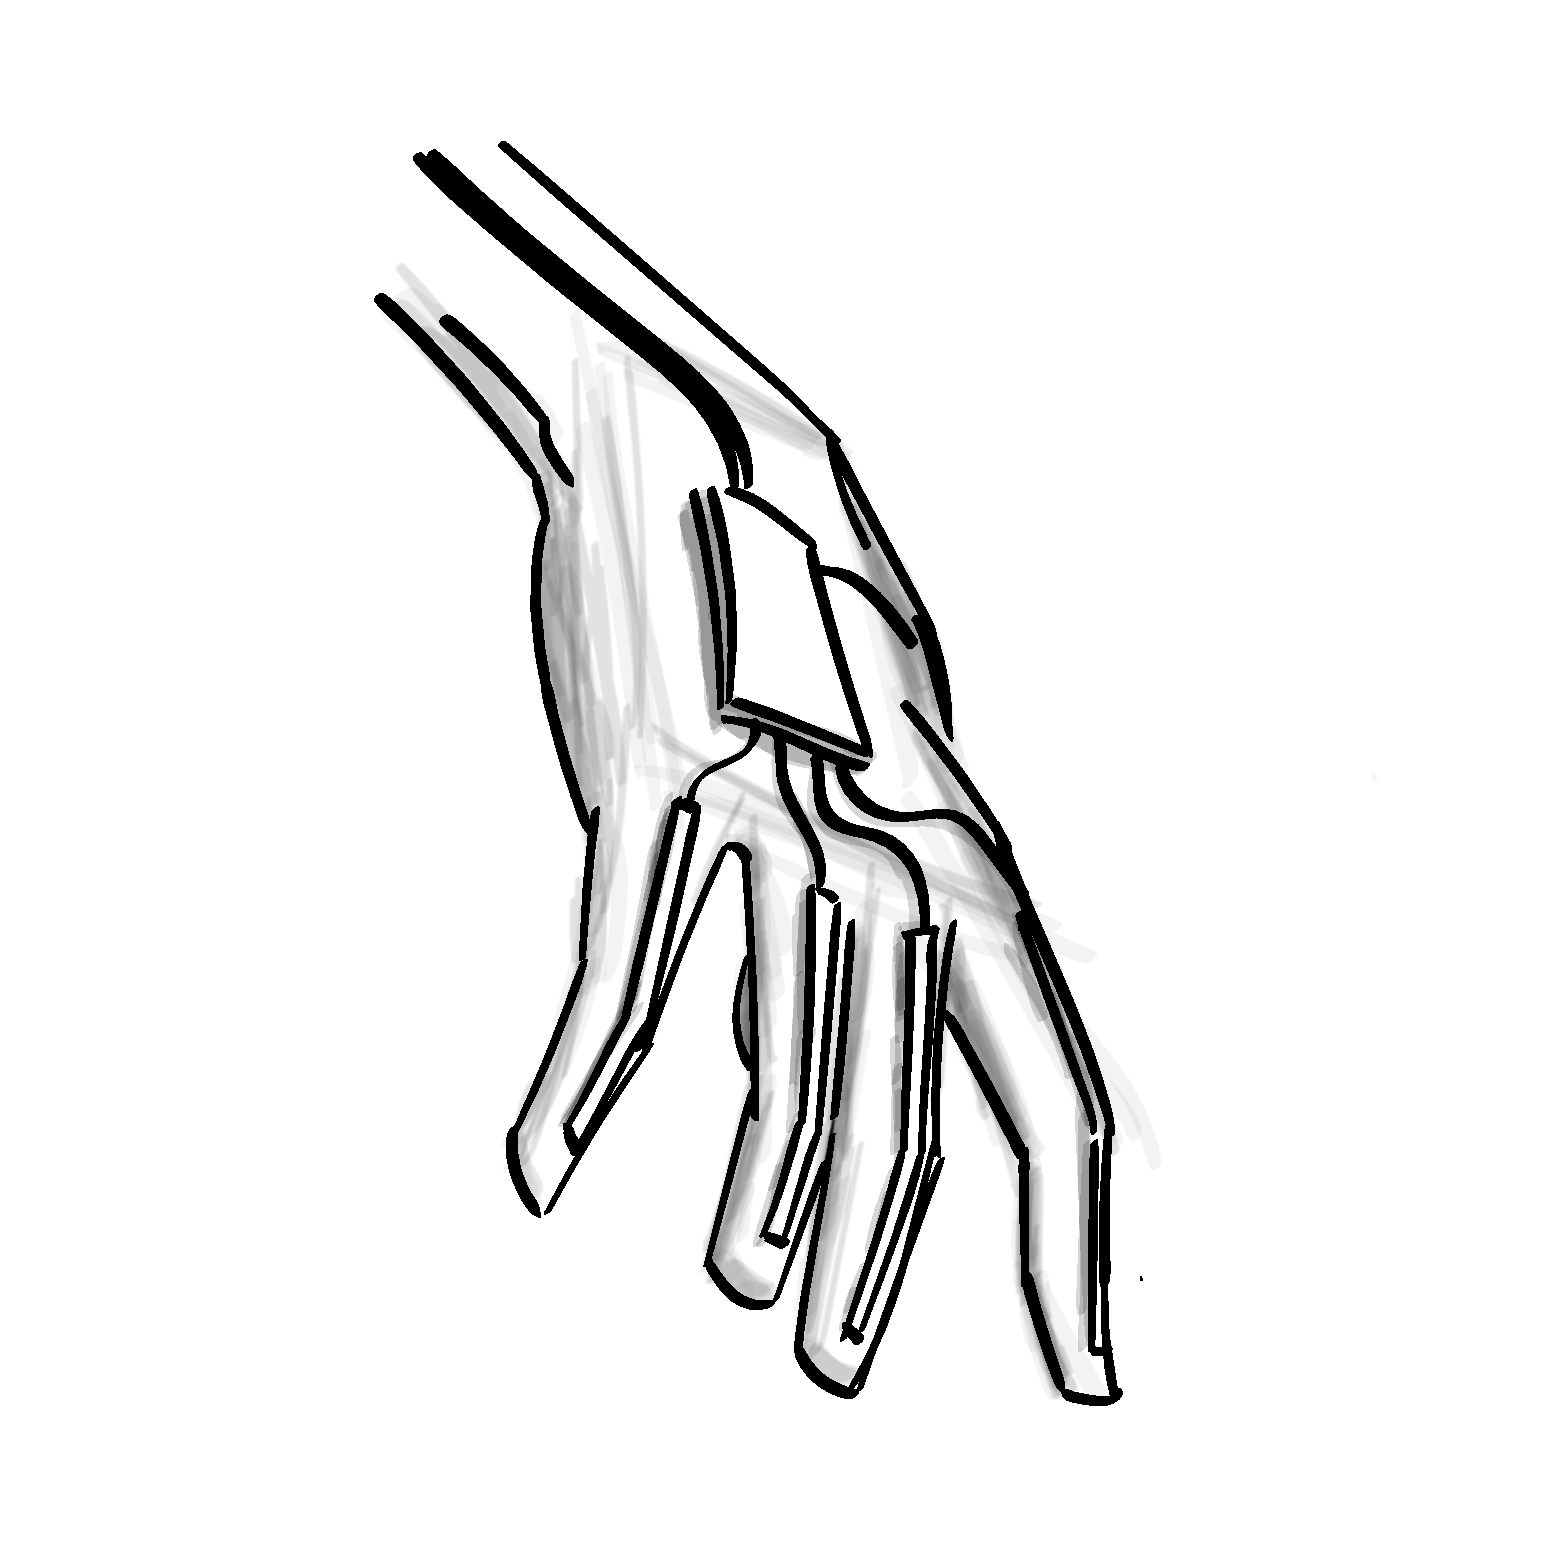
\includegraphics[page=1, width=\linewidth]{media/Ideasheet2.pdf}
            \subcaption{}\label{fig:IdeaFlexGlove}
        \end{minipage}
        \begin{minipage}[H]{.32\linewidth}
            \centering
            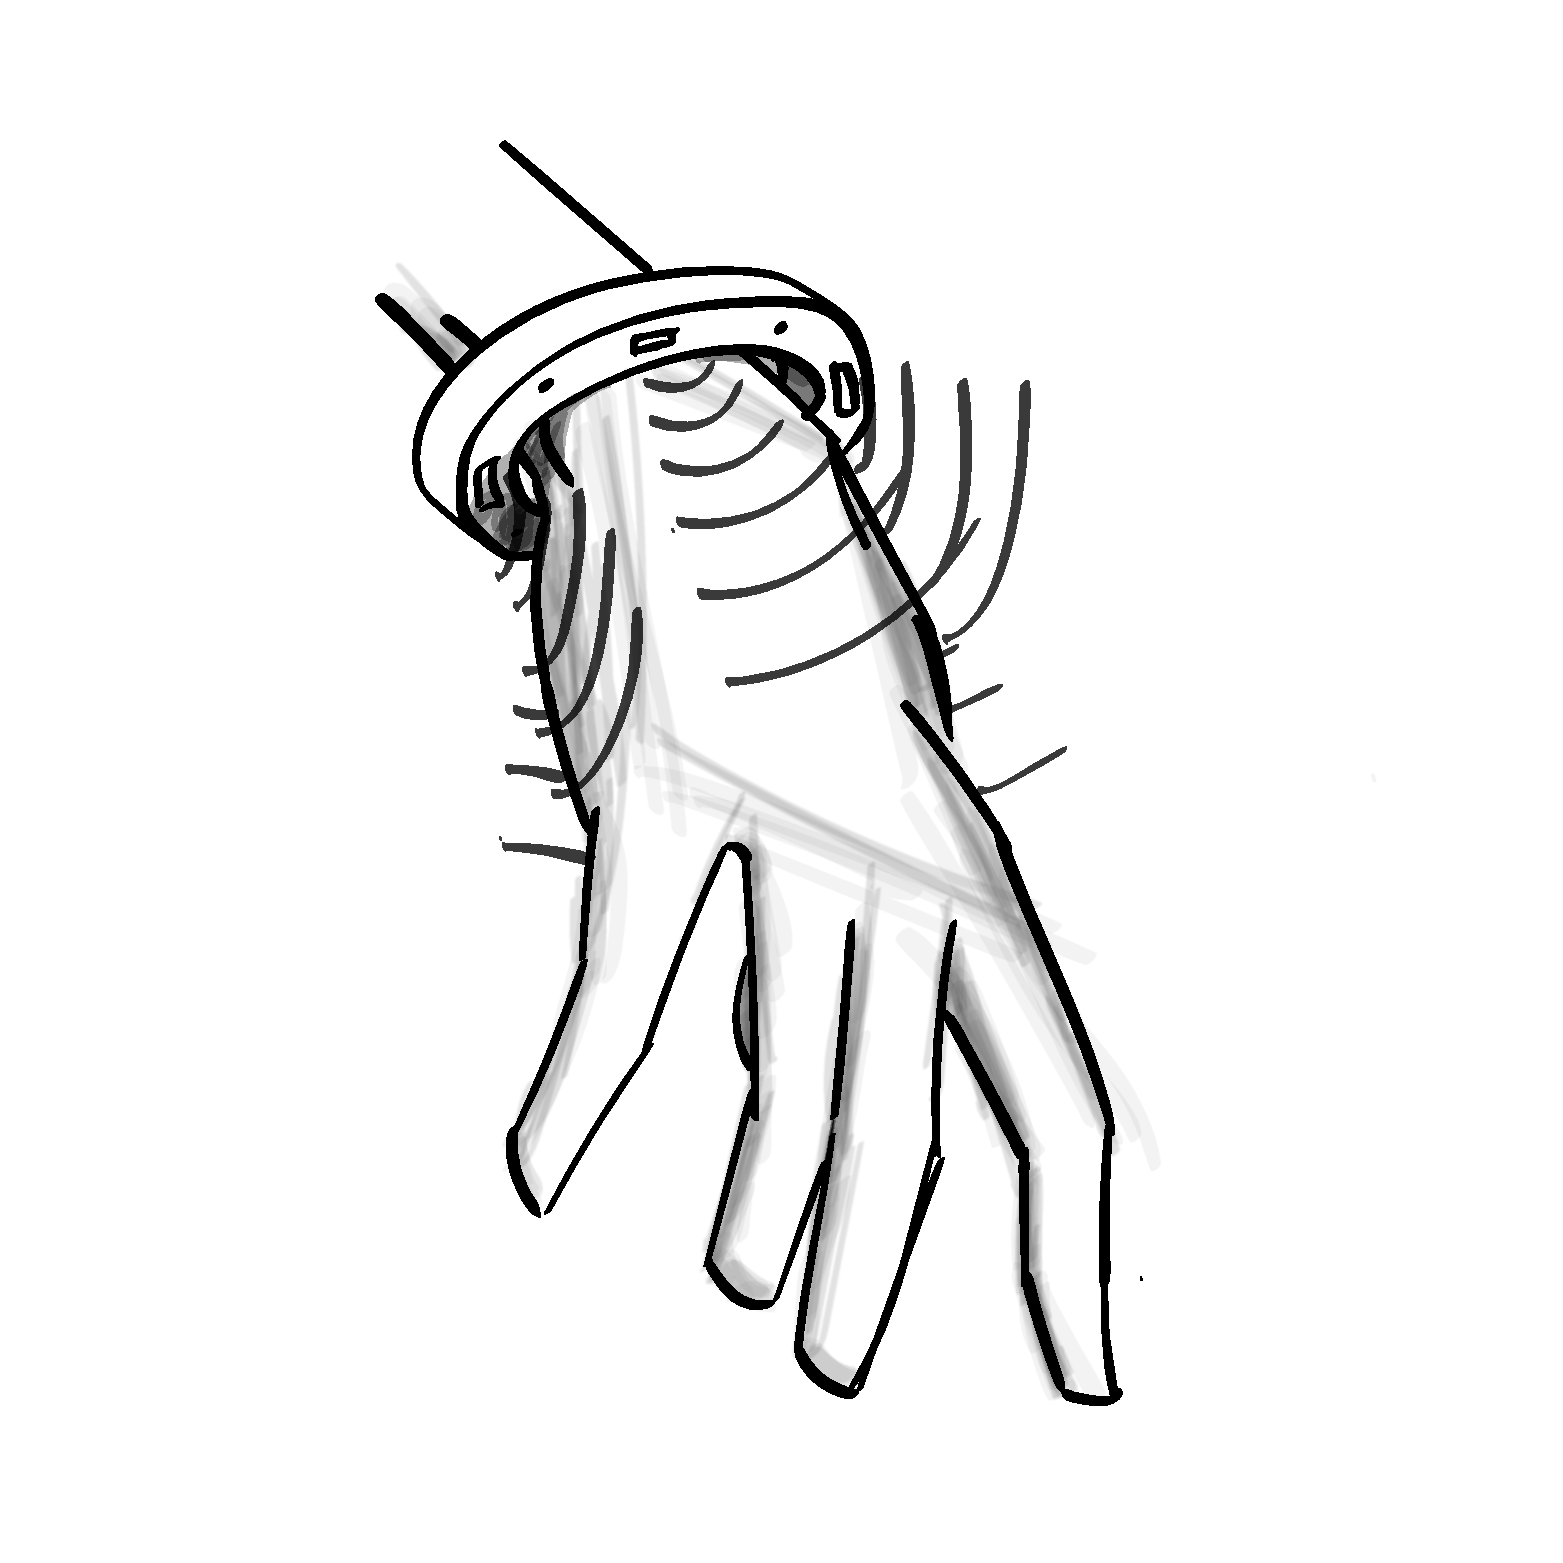
\includegraphics[page=1, width=\linewidth]{media/Ideasheet3.pdf}
            \subcaption{}\label{fig:IdeaRadarGlove}
        \end{minipage}
        \begin{minipage}[H]{.32\linewidth}
            \centering
            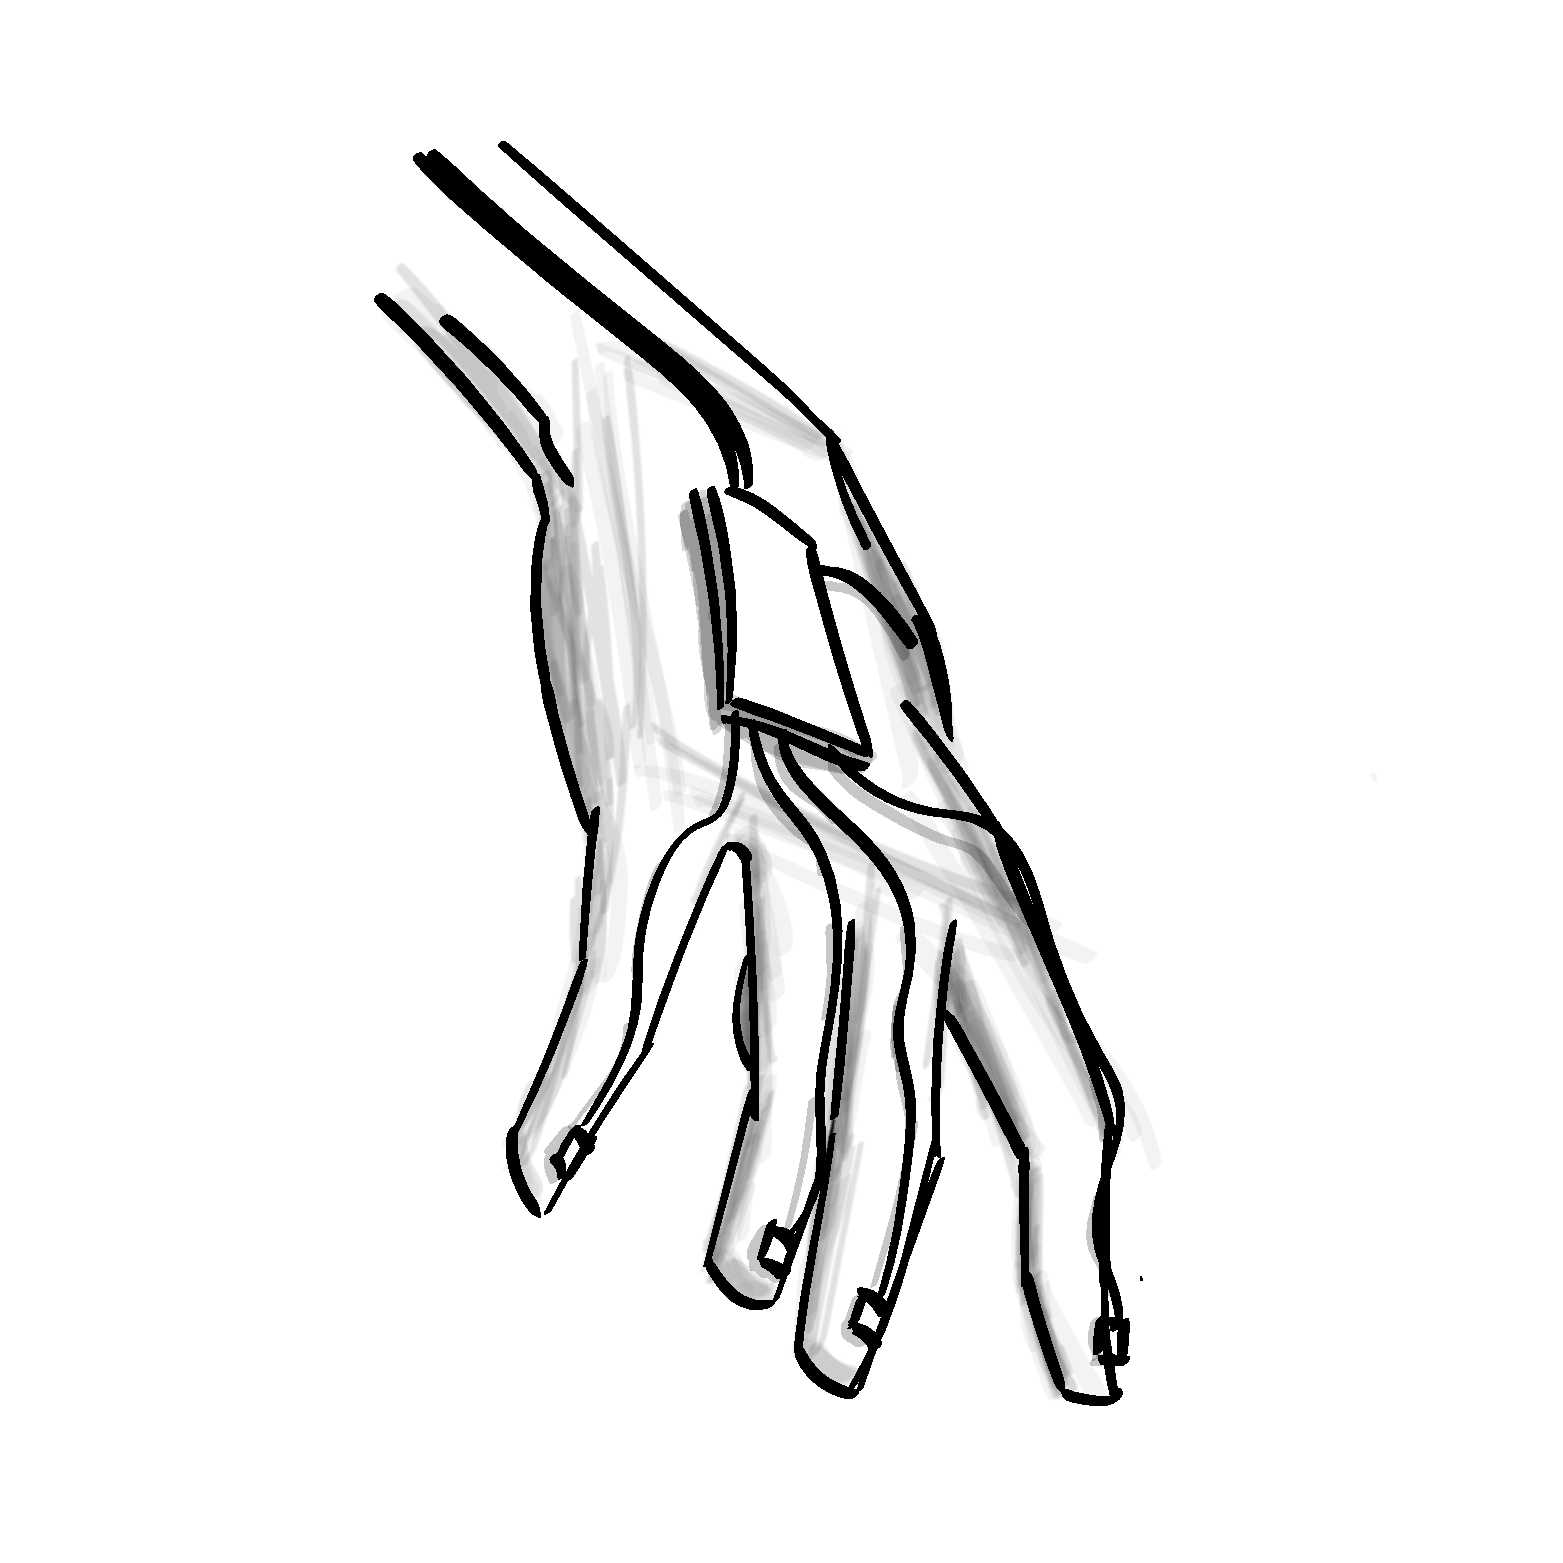
\includegraphics[page=1, width=\linewidth]{media/Ideasheet4.pdf}
            \subcaption{}\label{fig:IdeaMEMSGlove}
        \end{minipage}
        \begin{minipage}[H]{.32\linewidth}
            \centering
            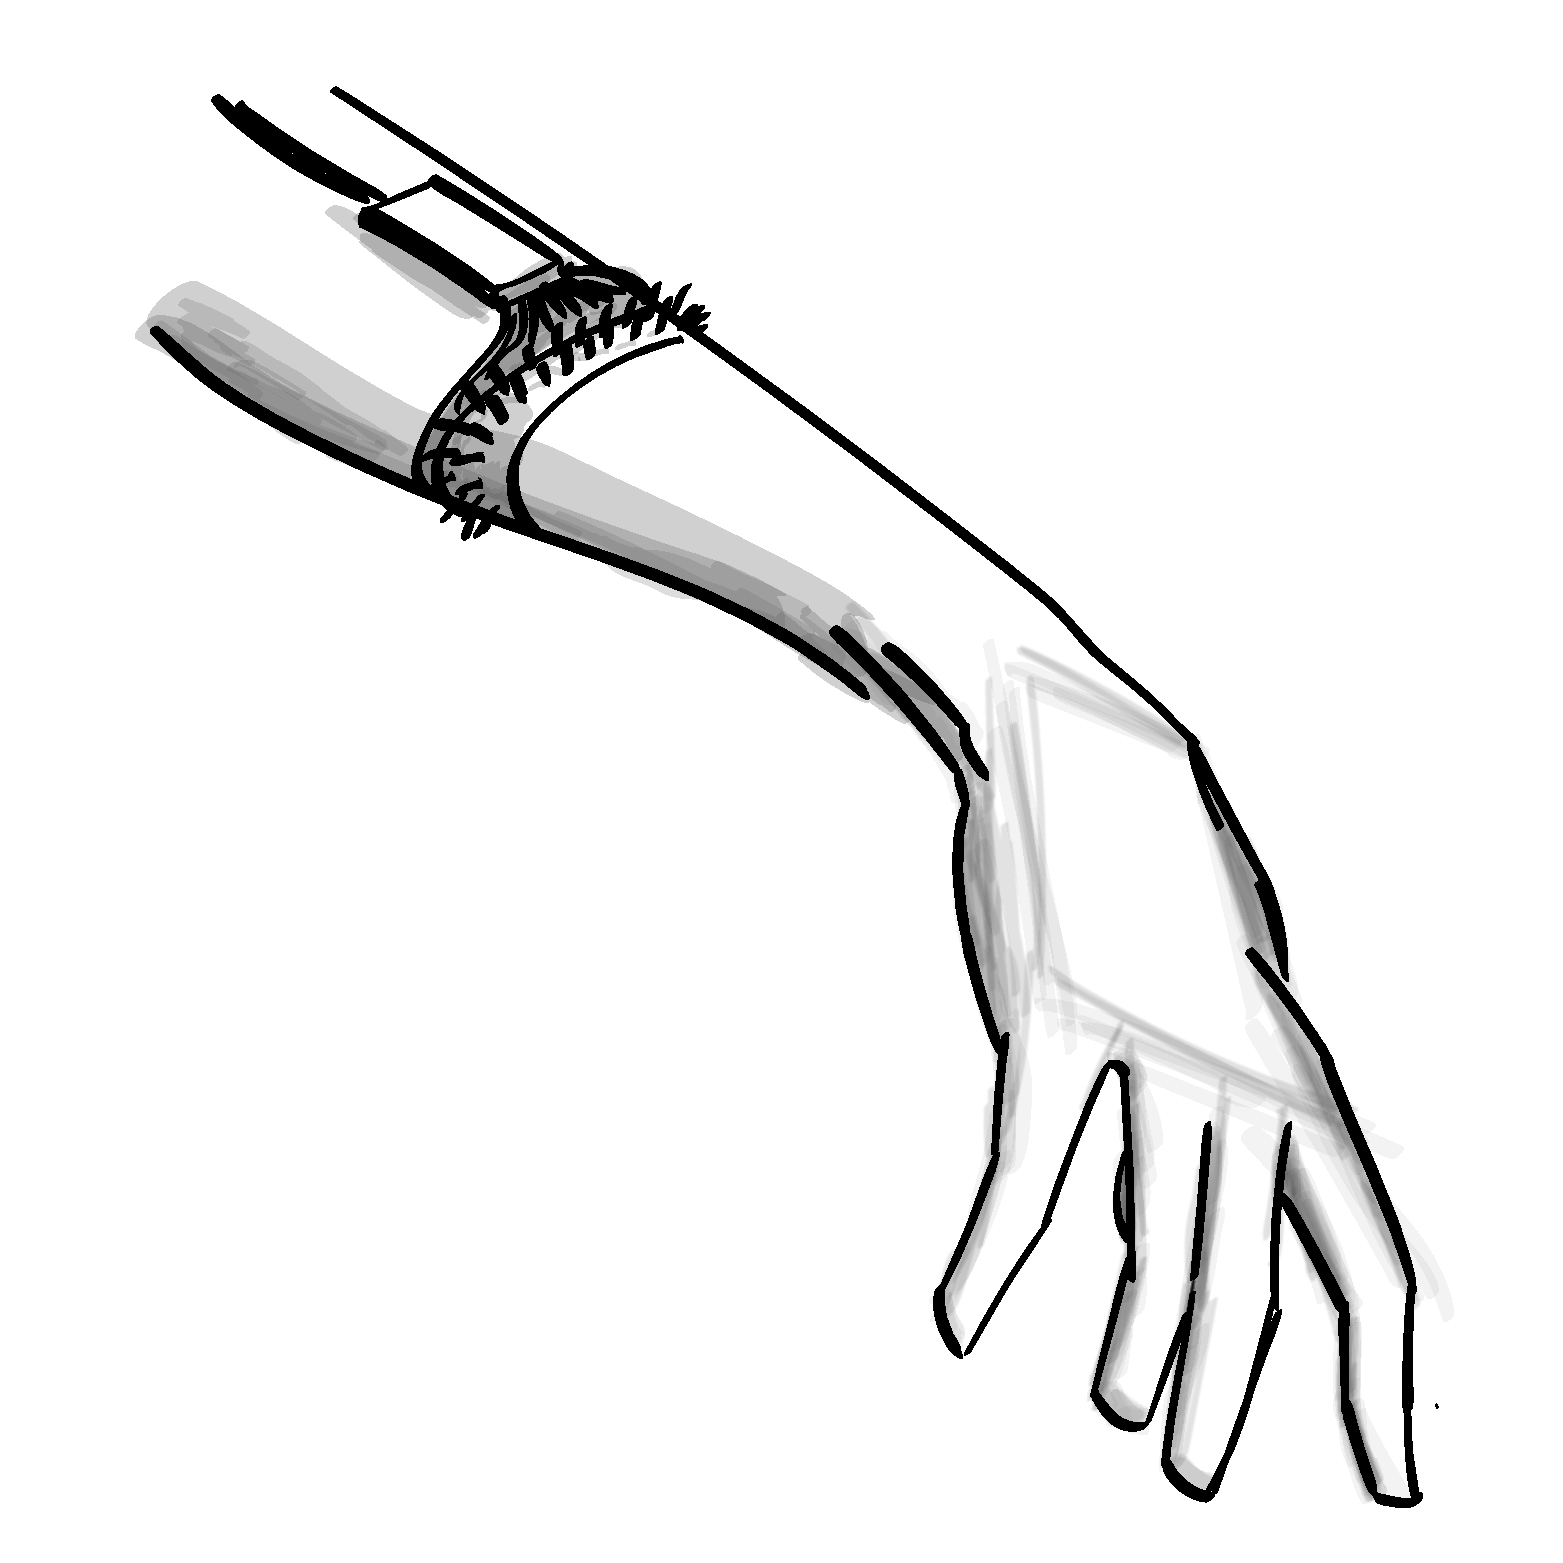
\includegraphics[page=1, width=\linewidth]{media/Ideasheet5.pdf}
            \subcaption{}\label{fig:IdeaNeedleEMGBand}
        \end{minipage}
        \begin{minipage}[H]{.32\linewidth}
            \centering
            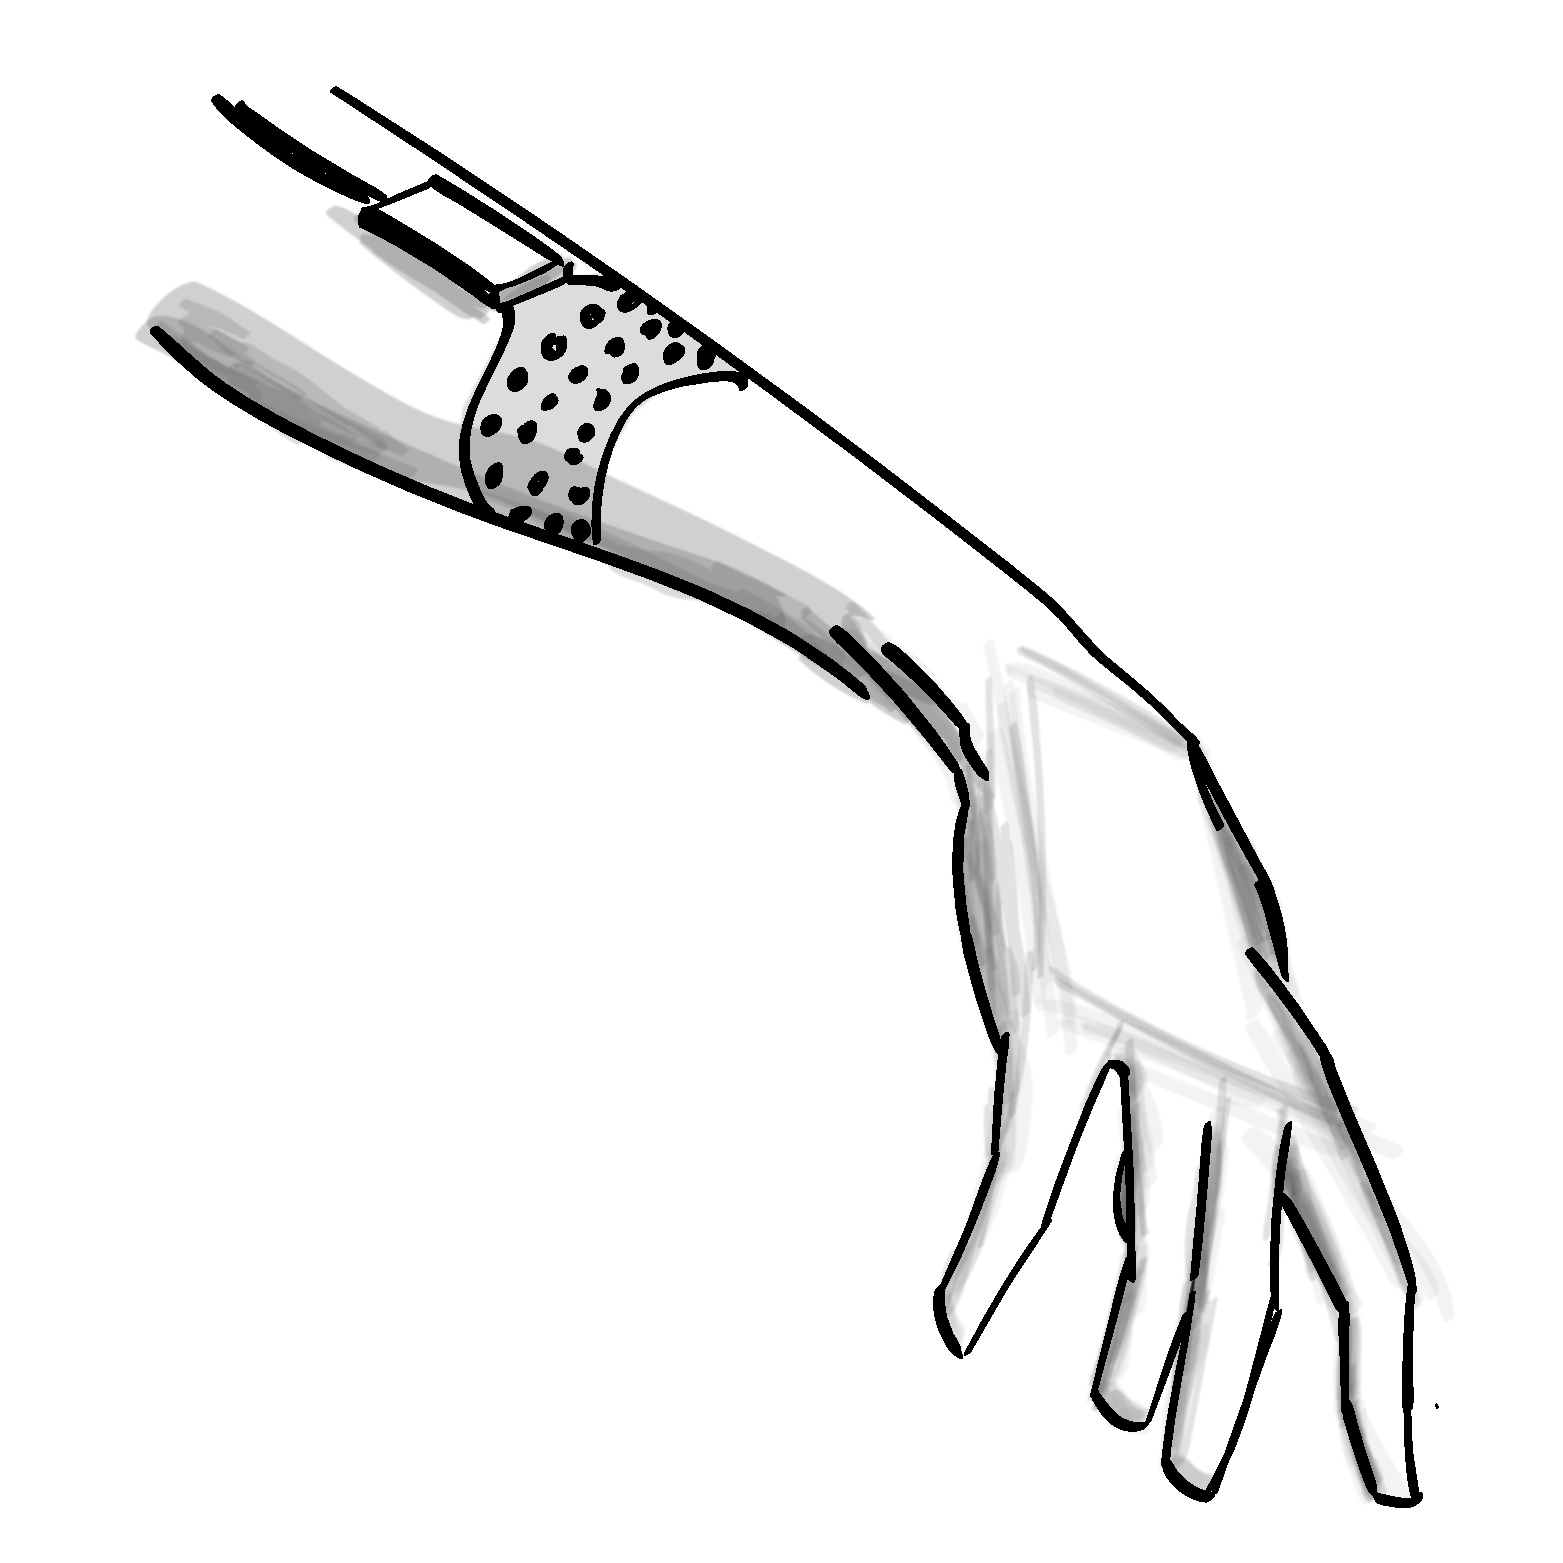
\includegraphics[page=1, width=\linewidth]{media/Ideasheet6.pdf}
            \subcaption{}\label{fig:IdeaSurfaceEMGBand}
        \end{minipage}
        \caption{Идеи}\label{fig:Idea}
    \end{figure}
    
    Как можно понять из раздела \emph{\ref{sec:IntroMotivation}}, я выбрал идею \ref{ItemDeltaChoice}\ref{ItemEMG}, а из её вариантов, разумеется, наименее инвазивный, то есть \emph{sEMG} \footnote{Surface Electromyography, поверхностная электромиография}, из-за условий эксплуатации, которые можно отнести к автомобильному классу\footcite[]{AutomotiveGrade:Wiki}\footnote{Имеется в виду класс надёжности компонентов, определяемый такими характеристиками, как стойкость к высоким температурам, вибрациям и другим физическим воздействиям} и даже к экстремальным.
    Недостатки этого выбора --- слабость исходного сигнала по сравнению с \emph{EMI} \footcite[Электромагнитные помехи]{EMI:Wiki} окружающей среды, но эта проблема легко решается продуманной конструкцией датчика.
    
    \subsection{Введение в теорию}\label{sec:IntroFiltersSignals}
    Сигнал служит для передачи информации; помехи, создаваемые другими источниками\footnote{Намеренными или нет} сигналов того же типа, могут исказить закодированную в нём информацию.
    В одних случаях помехи можно предотвратить, в других это оказывается невозможным или неэффективным.
    Считывание ЭМГ-сигнала относится ко второй категории случаев.
    В таких ситуациях используются фильтры\footnote{В разделе \ref{sec:SensorboardDesignInput} станет ясно, что речь идёт о частотном фильтре}.
    
    Фильтр с точки зрения обработки сигналов --- это устройство или процесс, способный удалять из поданного сигнала некоторые составляющие \footcite[]{Filter:Wiki}.
    С теоретической точки зрения разные типы фильтров можно описать математическим языком, а именно их передаточной функцией\footnote{Кроме того, не всякую функцию можно реализовать; это будет пояснено в разделе \ref{sec:MathAndPhysics}}.
    Чтобы не затягивать в этом разделе разговор о конкретике, нужно понять, что для работы абстракция должна быть реализована в реальном мире с использованием его свойств и явлений: как было выбрано ранее, для представления исходной модели я буду использовать электричество.

    Прежде чем разбираться, как работают реализации фильтров, нужно понять, как информация представляется с помощью электричества.
    В электронике повсеместно используются два способа представления информации: в цифровой и в аналоговой форме.
    \begin{figure}[H]
        \centering
        \begin{tikzpicture}
            \begin{axis}[
                axis x line=bottom,
                axis y line=middle,
                xlabel={$t[ms]$},
                ylabel={$U[{\mu}V]$},
                legend entries={$(a)$, $(b)$},
                legend pos=north east,
                height=.4\textwidth,
                width=.75\textwidth,
                clip=true,
                xtick distance=200,
                ytick distance=200,
                xmin=600,
                xmax=1600,
                ymin=-400,
                ymax=500,
                smooth,
                ymajorgrids=true,
                grid style=dashed,
                axis_style_default
            ]
                \addplot[
                    color=darkgray!75,
                    thick
                    ]
                    table {datasets/ecg_example_data/ecg_example_data};
                \addplot[
                    only marks,
                    color=red!75,
                    mark size=.275ex,
                    thick,
                    every mark/.append style={solid, fill=red!75, mark=*},
                    ]
                    table {datasets/ecg_example_data/ecg_bin_example_data};
            \end{axis}
        \end{tikzpicture}
        \caption{На графике показаны два сигнала ЭКГ \emph{(электрокардиограммы)} человека, считанные одним ЭМГ-датчиком \emph{(электромиографическим)}: аналоговый сигнал в $(a)$ и он же после оцифровки в $(b)$ \parenciteit{}{ECGDataThesis}\parenciteit{}{ECGData}}
        \label{fig:AnalogDigital}
    \end{figure}

    Как видно на рисунке \ref{fig:AnalogDigital}, аналоговому сигналу можно приписать свойство непрерывности: функция содержит бесконечное количество данных на ненулевом отрезке времени.
    Цифровой сигнал, напротив, периодически даёт нам одну точку: сигнал состоит из ограниченного количества\footnote{Оно может быть и нулевым, если выбрать отрезок времени короче периода дискретизации (sampling period)} данных на ненулевом отрезке времени.
    Кроме того, известно, что цифровой сигнал связан с аналоговым через \emph{оцифровку}, называемую также \emph{дискретизацией}\footcite[«Процесс перевода непрерывных функций, моделей, переменных и уравнений в их дискретные аналоги»]{Discretization:Wiki}, когда речь идёт скорее о математическом контексте.
    Разница между двумя способами представления информации будет подробнее рассмотрена в разделе \ref{sec:ProjectDesign}.
    Разделение сигналов на типы, разумеется, касается и тех частей, которые их преобразуют, например фильтров.

    На этом этапе знаний по теме достаточно, чтобы следить за дальнейшим изложением.

    \section{Характеристики проекта}\label{sec:ProjectCharacteristics}
    Зачастую в процессе проектирования трудно принимать решения.
    Чтобы сократить затраты времени, полезно начать с попытки определить важнейшие характеристики проекта, упорядочить их, конкретизировать и максимально количественно выразить, а затем выбрать только те, которые наиболее значимы.
    Нельзя забывать, что эта процедура, даже выполненная последовательно, всё равно может привести к цепочкам решений, которые закончатся невозможным или непрактичным проектом либо вообще ситуацией, описываемой словами: «\emph{Не то, чего хотелось}».
    Решение --- постоянно корректировать требуемые характеристики и проект, как только замечено отклонение.
    Вместо того чтобы воплощать идеи, держась за решения, основанные на исходных теоретических моделях и практическом опыте, которые не хочется признавать ложными, неадекватными или устаревшими, лучше сосредоточиться на том, что диктует в этом отношении реальность.

    \begin{figure}[H]
        \Centering
        \vspace{1ex}
        \textit{«Теория и практика иногда сталкиваются. И когда это происходит, теория проигрывает. Каждый раз.»}

        \RaggedLeft
        \vspace{1ex}

        \textit{\scriptsize{Linus B. Torvalds}}
        \vspace{1ex}
    \end{figure}

    Учитывая сложность проекта, я склоняюсь к выбору такого метода управления проектом\footnote{Управление работами по проекту}, который отчасти связываю с подходами к разработке программного обеспечения\footcite[]{SoftwareDevelopmentProcess:Wiki}.
    Я считаю, что подходы разработки ПО вполне можно использовать\footnote{Разумеется, с некоторыми изменениями} и для проектов, которые не ограничиваются областью информатики и не являются исключительно крупными по числу участников.
    \begin{figure}[H]
        \centering
        \begin{tikzpicture}[
            node distance = 2mm and 2mm,
            start chain = Waterfall going below right,
            every node/.style = {
                block,
                text width=16ex,
                minimum height=2.5em,
                inner sep=.25em,
                on chain=Waterfall,
                font_size
            },
        ]
            \node {Характеристики};
            \node {Проектирование};
            \node {Программирование и тестирование};
            \node {Интеграция системы};
            \node {Эксплуатация и сопровождение};
            \foreach \i [count=\j] in {2,...,5}{
                \draw[->, dashed] (Waterfall-\i) -| (Waterfall-\j);
                \draw[->] (Waterfall-\j) -| (Waterfall-\i);
            }
            \draw \InvisibleBorder;
        \end{tikzpicture}
        \caption{Каскадная модель (Waterfall) разработки программного обеспечения}
        \label{fig:Waterfall}
    \end{figure}
    Со временем каскадная модель (Waterfall) проектирования ПО\footcite[]{WaterfallModel:Wiki} \emph{(рисунок \ref{fig:Waterfall})} оказалась утопичной и неэффективной для реального мира и была заменена гораздо более новыми, эффективными и гибкими подходами, такими как Agile\footcite[]{AgileModel:Wiki}, Scrum\footcite[]{ScrumModel:Wiki} и DevOps\footcite[]{DevOpsModel:Wiki}.
    Совет быть гибким в «\emph{Requirements}»\footnote{То есть в характеристиках, целях} и «\emph{Design}»\footnote{Решения и обоснования «\emph{Requirements}»} и стараться менять характеристики проекта, приспосабливая его к влиянию реального мира, --- это как раз та философия современных подходов, которую я стараюсь применять в своём методе работы.

    \noindent Основные характеристики проекта:
    \begin{enumerate}[label=\emph{(\arabic*)}]
        \item Уметь делать то, для чего он задуман: \emph{надёжно считывать, преобразовывать и передавать сигнал} \label{char:Reliability}
        \item По возможности \emph{не стеснять движения} кисти и руки своими \emph{размерами} и \emph{весом} \label{char:CompactNoDriveImpact}
        \item Быть достаточно \emph{компактным}, чтобы помещаться под курткой \label{char:Compact}
        \item Обладать некоторой \emph{ремонтопригодностью}, не сильно жертвуя характеристикой \ref{char:Compact} \label{char:Repairability}
        \item Быть \emph{удобным} в использовании, не царапать руку, не отвлекать человека \label{char:ComfortableNoPain}
        \item Иметь время \emph{работы} более 5 часов \label{char:Automaticity}
        \item Обеспечивать \emph{интуитивное управление} транспортным средством \label{char:IntuitiveControl}
        \item Не быть помехой в \emph{стрессовых} ситуациях \label{char:StressReactionAdapted}
        \item Быть \emph{устойчивым к внешним факторам}, таким как удары, вода, отсутствие потока воздуха \label{char:ExternalImpactAdapted}
        \item Позволять настраивать нужные жесты \label{char:GestureVariability}
    \end{enumerate}
    \todo{проверить ссылки в документе на пункты выше}
    Некоторые пункты могут показаться не относящимися к проектированию такой небольшой части, как датчик, но причина в том, что список является результатом не линейной разработки, а итераций гибкого подхода к проектированию, и каждый приведённый выше пункт влияет на проект\footnote{Некоторые пункты будут упомянуты со ссылкой в более конкретных разделах, например \ref{sec:ProjectDesignAbstractModel} или \ref{sec:MotherboardDesign}}. \todo{исправить после предыдущей правки}

    \section{Проектирование системы}\label{sec:ProjectDesign}
    Modus operandi\footnote{Тактика, привычный образ действий}, применяемый в этом разделе, --- абстракция: она состоит в упрощении исходной идеи до общей модели и её последующей постепенной конкретизации.

    \subsection{Абстрактная модель}\label{sec:ProjectDesignAbstractModel}
    Пульт управления удобно представить в виде структурной схемы\footcite[]{BlockDiagram:Wiki} \emph{(рисунок \ref{fig:BlockDiagram})}, чтобы понять, какую архитектуру\footnote{Имеется в виду модель реализации} и реализацию системы выбрать.
    \begin{figure}[H]
        \centering
        \begin{tikzpicture}[auto,>=latex', font_size, box_width/.style={minimum width=5em}]
            \draw (0,0)
                node at (0,0) (input) {\textit{ЭМГ-сигнал}};
            \draw (input)
                node[box_width, block] at ++(2.2,0) (block_analogue1) {Аналог.};
            \draw[->] (input.east) -- (block_analogue1.west);
            \draw (block_analogue1)
                node[box_width, block] at ++(2.2,0) (block_intermediate1) {A$\Rightarrow$D}
                [->] (block_analogue1.east) -- (block_intermediate1.west);
            \draw (block_intermediate1)
                node[box_width, block] at ++(2.2,0) (block_digital) {Цифр.}
                [->] (block_intermediate1.east) -- (block_digital.west);
            \draw (block_digital)
                node[box_width, block] at ++(2.2,0) (block_intermediate2) {D$\Rightarrow$DcA}
                [->] (block_digital.east) -- (block_intermediate2.west);
            \draw (block_intermediate2)
                node[box_width, block] at ++(2.2,0) (block_analogue2) {Аналог.}
                [->] (block_intermediate2.east) -- (block_analogue2.west);
            \draw (block_analogue2)
                node at ++(2.2,0) (output) {\textit{RF}}
                [->] (block_analogue2.east) -- (output.west);
            \draw \InvisibleBorder;
        \end{tikzpicture}
        \caption{}
        \label{fig:BlockDiagram}
    \end{figure}
    Как видно, \emph{Input} --- это ЭМГ-сигнал, и чтобы дойти до радиоканала связи, соответствующего \emph{Output}, сигнал должен пройти через ряд преобразований.
    % TRANSLATOR NOTE: block names abbreviated to "Аналог." / "Цифр." (also in the tikz block diagrams) so the boxes keep their original widths; "DcA" (Italian "Digitale codificato in Analogico") kept and glossed in the footnote.
    Цепочка преобразований содержит блок «\emph{Аналог.}», который представляет часть, непрерывно преобразующую сигнал, блок «\emph{A$\Rightarrow$D}», оцифровывающий сигнал, блок «\emph{Цифр.}», дискретно преобразующий информацию, и блок «\emph{D$\Rightarrow$DcA}»\footnote{«DcA» --- от итальянского \emph{Digitale codificato in Analogico}, то есть «цифровое, закодированное в аналоговое»}, который кодирует цифровую информацию в другую форму\footnote{С помощью метода, называемого «\emph{модуляцией}» \parencite[]{Modulation:Wiki} сигнала}, пригодную для передачи по радиоканалу.

    \noindent Возникает вопрос: почему бы не убрать блоки «\emph{A$\Rightarrow$D}», «\emph{Цифр.}» и «\emph{D$\Rightarrow$DcA}» и не заменить всю схему одним блоком «\emph{Аналог.}»\footnote{Он представляет преобразование аналогового сигнала в радиосигнал без оцифровки и без какой-либо модуляции (что меняет и способ передачи информации: без метода модуляции, поскольку сигнал отсутствует в цифровой форме)}?

    \nopagebreak
    \noindent Причины:
    \begin{enumerate}[label=\emph{(\arabic*)}]
        \item Нынешняя непрактичность.
        Многие вычисления, как правило, выполняются на цифровых устройствах, и поэтому на рынке нельзя найти аналоговые решения с сопоставимой стоимостью и вычислительной мощностью.
        \item Вторая причина --- точность и устойчивость системы к внешним факторам.
        Сигнал, представленный в аналоговой форме, содержит бесконечно больше информации\footnote{Разницу можно увидеть в разделе \ref{sec:IntroFiltersSignals}} \footnote{У сигналов, преобразованных из цифрового представления в аналоговое, недостающая информация заполняется} по сравнению со своей оцифрованной формой и легко может быть искажён при обработке или передаче.
        Для представления цифрового сигнала обычно используется двоичная система: исказить сигнал, который, например, использует половину своей амплитуды для «1», а другую половину для «0», гораздо менее вероятно, чем значение, закодированное в бесконечно малой доле амплитуды.
        Кроме того, для изменения сигнала используются электронные компоненты\footnote{Это будет рассмотрено подробнее в разделе \ref{sec:MathAndPhysics}}, которые в реальном мире обладают несовершенствами, представимыми в виде дополнительных элементов, называемых паразитными \emph(рисунок \ref{fig:ExampleParassiticElements}), и из-за природы аналогового сигнала они влияют на информацию гораздо сильнее и непредсказуемым образом\footnote{Цифровой сигнал тоже искажается при обработке, но последствия можно устранить схемами вроде триггера Шмитта\parenciteit{}{SchmittTrigger:Wiki}, тогда как для аналогового сигнала это неприменимо}.
        То же самое относится к радиопередаче: сигнал без модуляции, то есть не оцифрованный, будет менее устойчив к EMI.
        \item Третья причина в том, что не все функции можно реализовать: например, невозможно реализовать в виде сети аналоговых компонентов недетерминированные функции\footnote{Сохраняя аналоговый режим работы схемы}, и трудно или невозможно --- функции, описывающие системы TV\footnote{Time-variant, то есть изменяющиеся во времени}\:\footcite[]{TimeVariantSystem:Wiki}.
    \end{enumerate}

    \begin{figure}[H]
        \centering
        \begin{minipage}[H]{.4\linewidth}
            \centering
            \begin{tikzpicture}[transform shape, use fpu reciprocal]
                \draw (0,0)
                    node[left]{$A$}
                    to[short, o-] ++(.5,0)
                    to[R, l=$R$] ++(2,0)
                    to[short, -o] ++(.5,0)
                    node[right]{$B$};
            \end{tikzpicture}
            \subcaption{Простое представление резистора номиналом $R$}
            \label{fig:ExampleParassiticElementsSimple}
        \end{minipage}
        \hspace*{0.04\linewidth}
        \begin{minipage}[H]{.4\linewidth}
            \centering
            \begin{tikzpicture}[transform shape, use fpu reciprocal]
                \draw (0,0)
                    node[left]{$A$}
                    to[short, o-] ++(1,0)
                    coordinate(AR)
                    to[R, l=$R$, -*] ++(2,0)
                    coordinate(RL)
                    to[L, l=$L_p$] ++(2,0)
                    to[short, -o] ++(.5,0)
                    node[right]{$B$};
                \draw (AR)
                    to[short, *-] ++(0,1.25)
                    to[C, l=$C_p$] ++(2,0)
                    -- (RL);
            \end{tikzpicture}
            \subcaption{Более точное представление резистора номиналом $R$, на который могут влиять $C_p$ и $L_p$ --- паразитные ёмкость и индуктивность}
            \label{fig:ExampleParassiticElementsRefined}
        \end{minipage}
        \caption{Пример двух моделей резистора}
        \label{fig:ExampleParassiticElements}
    \end{figure}

    \noindent Возникает второй вопрос: почему бы не убрать оба блока «\emph{Аналог.}»?

    \nopagebreak
    \noindent Причины:
    \begin{enumerate}[label=\emph{(\arabic*)}]
        \item Блок «\emph{A$\Rightarrow$D}» требует, а блок «\emph{D$\Rightarrow$DcA}» выдаёт сигнал в точно заданных пределах напряжения: поэтому необходимо согласовать напряжение сигнала, прежде чем передавать его дальше.
        \item Сигнал всегда загрязнён шумом, и если оцифровать его без аналоговой фильтрации, есть риск искажения данных\footnote{Это может привести к сбою системы, если данные обрабатываются напрямую, или к сокращению количества информации, если используются реализации цифровых фильтров}.
        \item Аналоговая реализация фильтра стоит дешевле цифровой той же эффективности.
        \item Объём данных, собираемых и обрабатываемых в дискретной форме, напрямую связан с вычислительной мощностью и скоростью: с ростом объёма обрабатываемых данных цифровому фильтру для работы нужна большая вычислительная мощность, тогда как аналоговый фильтр от этого никак не зависит. \label{reas:SamplingRateVsDigitalAnalogFilters}
        \item Как следует из пункта \ref{reas:SamplingRateVsDigitalAnalogFilters}, аналоговая реализация фильтра в большинстве случаев\footnote{Зависит от частоты сбора дискретных данных} потребляет меньше энергии\footnote{Это станет ясно в разделе \ref{sec:ProjectDesignAbstractModel}}, чем цифровая той же эффективности.
        \item При оцифровке нефильтрованного сигнала выше риск клиппинга\footnote{Выход за заданные пределы напряжения схемы, выполняющей оцифровку, что обычно ведёт к потере части данных} \footnote{Этого можно избежать, расширив верхний и нижний пределы схемы оцифровки, но тогда начинает снижаться разрешение сигнала; чтобы его сохранить, придётся выбрать другую, более дорогую схему оцифровки} сигнала.
    \end{enumerate}

    \subsection{Модель реализации}\label{sec:ProjectDesignImplementationModel}
    Модель реализации --- это максимально конкретная модель до выбора конкретных компонентов реализации; она может помочь увидеть все возможности непосредственно перед их выбором.

    Количество ЭМГ-сигналов зависит от мышц, с которых нужно снимать информацию.
    Эта информация определяется жестами\footnote{Система должна быть гибкой, чтобы можно было настраивать нужные жесты}, которые нужно распознавать; поэтому\footnote{Ссылка на характеристику проекта «\ref{char:GestureVariability}» в разделе \ref{sec:ProjectCharacteristics}} количество электродов --- концептуальной части, ближайшей к съёму сигнала, --- должно быть переменным.
    Передавать сигнал в том виде, в каком его воспринимают электроды, --- плохая идея из-за слабости сигнала по сравнению с EMI окружающей среды.
    Следовательно, сигнал нужно усилить перед передачей, но потеря информации в аналоговом сигнале всё равно остаётся.
    Чтобы точность информации была менее чувствительна к EMI, рекомендуется оцифровывать сигнал перед передачей.
    Только что описанное решение увеличивает стоимость устройства из-за цены отдельных АЦП\footnote{Analog to digital converter, аналого-цифровой преобразователь (ADC)}, которых к тому же должно быть много и одноканальных\footnote{Это снижает возможность использовать АЦП с мультиплексорами \parenciteit{}{Multiplexer:Wiki}, позволяющими использовать на нескольких каналах ту часть, которая реализует схему оцифровки и является самой дорогой частью микросхемы}, но надёжность схемы для меня важнее\footnote{Ссылка на характеристику проекта «\ref{char:Reliability}» в разделе \ref{sec:ProjectCharacteristics}}.

    Цифровую часть, в отличие от аналоговой и оцифровывающей частей, не нужно децентрализовать, в том числе из-за тенденции к более высокой стоимости\footnote{В нашем случае это сложные части, содержащие память, процессор и другие компоненты, которые пришлось бы дублировать в каждом дополнительном чипе (тем самым увеличивая стоимость)} при использовании нескольких чипов вместо одного и из-за роста задержек связи\footnote{Если их хочется избежать, придётся выбирать более специализированные чипы, что опять увеличивает стоимость}.

    Для модулятора и усилителя радиосигнала можно использовать готовые чипы, реализующие обе функции сразу: это снижает затраты, но уменьшает гибкость в выборе используемых протоколов связи и дальности устройства.
    Такой выбор вполне возможен и логичен, поскольку нет особой необходимости поддерживать много протоколов или работать на различных расстояниях.
    Кроме того, чип, отвечающий за модуляцию, иногда встроен прямо в схемы, которые относятся к категории цифровой части\footnote{SoC \parenciteit{}{SoC:Wiki}, микроконтроллеры}.
    Решение объединить модулятор, усилитель сигнала и цифровую часть может снизить задержку и увеличить скорость передачи данных системы благодаря параллельному интерфейсу, часто используемому внутри кремния чипов, который к тому же дешевле интерфейсов между разными кристаллами, выходящих за пределы чипа\footnote{Чаще всего это $I_2 C$ \parenciteit{}{I2C:Wiki} и $SPI$ \parenciteit{}{SPI:Wiki}}, однако именно этот вопрос будет конкретизирован далее в разделе \ref{sec:MotherboardDesignInterface}.

    \noindent В итоге рассуждений мы получаем две схемы, показанные на рисунке \ref{fig:ConcretizedBlockDiagram}
    \nopagebreak
    \begin{figure}[H]
        \centering
        \begin{minipage}[H]{\linewidth}
            \centering
            \begin{tikzpicture}[auto,>=latex', font_size, box_width/.style={minimum width=5.5em}]
                \foreach \n in {1,2}{
                    \node at (0,-\n+2) (input\n) {\textit{ЭМГ-сигнал \n}};
                };
                \node at (0,-3+2) (input3) {\textit{ЭМГ-сигнал n}};
                \foreach \n in {1,2,3}{
                    % \node at (0,-\n+2) (input\n) {\textit{Segnale EMG\n}};
                    \node[box_width, block] at ++(3,-\n+2) (block_analogue1_\n) {Аналог., A$\Rightarrow$D};
                    \draw[->] (input\n.east) -- (block_analogue1_\n.west);
                };
                \draw (block_analogue1_2)
                    node[box_width, block] at ++(3.25,0) (block_digital) {Цифр.};
                \foreach \n in {1,2}{
                    \draw ($(block_analogue1_\n.east)!.5!(block_digital.west)$)
                        coordinate(iter_arrow_\n)
                        [-] (block_analogue1_\n.east) -- (iter_arrow_\n |- block_analogue1_\n.east)
                        coordinate(iter_arrow_end_\n);
                };
                \draw ($(block_analogue1_3.east)!.5!(block_digital.west)$)
                        coordinate(iter_arrow_3)
                        [dashed] (block_analogue1_3.east) -- (iter_arrow_3 |- block_analogue1_3.east)
                        coordinate(iter_arrow_end_3);
                \draw[-] (iter_arrow_end_1) -- (iter_arrow_end_2);
                \draw[dashed] (iter_arrow_end_2) -- (iter_arrow_end_3);
                \draw[->] (iter_arrow_end_2) -- (block_digital.west);
                \filldraw (iter_arrow_end_2) circle (1pt);
                \draw (block_digital)
                    node[box_width, block] at ++(3,0) (block_intermediate2) {D$\Rightarrow$DcA, Аналог.}
                    [->] (block_digital.east) -- (block_intermediate2.west);
                \draw (block_intermediate2)
                    node at ++(2.5,0) (output) {\textit{RF}}
                    [->] (block_intermediate2.east) -- (output.west);
                \draw \InvisibleBorder;
            \end{tikzpicture}
            \subcaption{Модель, в которой модулятор и усилитель сигнала отделены от цифровой части}
            \label{fig:ConcretizedBlockDiagramMulti}
        \end{minipage}
        \begin{minipage}[H]{\linewidth}
            \centering
            \begin{tikzpicture}[auto,>=latex', font_size, box_width/.style={minimum width=5.5em}]
                \foreach \n in {1,2}{
                    \node at (0,-\n+2) (input\n) {\textit{ЭМГ-сигнал \n}};
                };
                \node at (0,-3+2) (input3) {\textit{ЭМГ-сигнал n}};
                \foreach \n in {1,2,3}{
                    % \node at (0,-\n+2) (input\n) {\textit{Segnale EMG\n}};
                    \node[box_width, block] at ++(3,-\n+2) (block_analogue1_\n) {Аналог., A$\Rightarrow$D};
                    \draw[->] (input\n.east) -- (block_analogue1_\n.west);
                };
                \draw (block_analogue1_2)
                    node[box_width, block] at ++(4,0) (block_digital) {Цифр., D$\Rightarrow$DcA, Аналог.};
                \foreach \n in {1,2}{
                    \draw ($(block_analogue1_\n.east)!.5!(block_digital.west)$)
                        coordinate(iter_arrow_\n)
                        [-] (block_analogue1_\n.east) -- (iter_arrow_\n |- block_analogue1_\n.east)
                        coordinate(iter_arrow_end_\n);
                };
                \draw ($(block_analogue1_3.east)!.5!(block_digital.west)$)
                        coordinate(iter_arrow_3)
                        [dashed] (block_analogue1_3.east) -- (iter_arrow_3 |- block_analogue1_3.east)
                        coordinate(iter_arrow_end_3);
                \draw[-] (iter_arrow_end_1) -- (iter_arrow_end_2);
                \draw[dashed] (iter_arrow_end_2) -- (iter_arrow_end_3);
                \draw[->] (iter_arrow_end_2) -- (block_digital.west);
                \filldraw (iter_arrow_end_2) circle (1pt);
                \draw (block_digital)
                    node at ++(3,0) (output) {\textit{RF}}
                    [->] (block_digital.east) -- (output.west);
                \draw \InvisibleBorder;
            \end{tikzpicture}
            \subcaption{Модель, в которой модулятор и усилитель сигнала объединены с цифровой частью}
            \label{fig:ConcretizedBlockDiagramMono}
        \end{minipage}
        \caption{Абстрактные модели проекта, максимально конкретизированные без окончательного выбора компонентов}
        \label{fig:ConcretizedBlockDiagram}
    \end{figure}
    Отныне для обозначения концептуального объединения блоков я буду использовать термины «сенсорная плата» для блоков «\emph{Аналог.}», «\emph{A$\Rightarrow$D}» и «основная плата»\footnote{Объединяет все блоки, которые существуют в единственном экземпляре и не требуют размещения в определённом месте} для блоков «\emph{Цифр.}», «\emph{D$\Rightarrow$Dca}», «\emph{Аналог.}»: граница между двумя понятиями проходит по интерфейсу от блока «\emph{A$\Rightarrow$D}» к блоку «\emph{Цифр.}».

    \subsection{Организация последующих частей}
    В нашем случае конкретизацию реализаций проще начать с основной платы\footnote{Пояснено в конце раздела \ref{sec:ProjectDesignImplementationModel}}, которая существует в единственном экземпляре, может объединять несколько блоков и с точки зрения выбора менее гибка, чем сенсорная плата\footnote{Пояснено в конце раздела \ref{sec:ProjectDesignImplementationModel}}.
    Сенсорная плата проектируется преимущественно на уровне SMD-компонентов\footcite[]{SMT:Wiki} и выводных (TH) компонентов\footcite[]{THT:Wiki}, тогда как для основной платы мы можем выбирать только готовые решения\footnote{Чтобы уменьшить размеры и стоимость, я предпочёл бы не добавлять функциональность сверх той, что предоставляет основной чип (и, возможно, модулятор)}.
    Кроме того, хотя основная плата не входит в тему выпускной работы \emph{maturit\`{a}}, она влияет на выбор цифрового протокола передачи информации о сигнале от сенсорной платы к основной и играет незаменимую роль как в окончательной версии датчика, так и в модели прототипа: поэтому её тоже нужно конкретизировать.

    \section{Основная плата}\label{sec:Motherboard}
    \begin{samepage}
        \subsection{Характеристики}\label{sec:MotherboardCharacteristics}
            Основная плата, то есть совокупность блоков «\emph{Цифр.}», «\emph{D$\Rightarrow$DcA}», «\emph{Аналог.}», должна соответствовать следующим характеристикам:
            \begin{enumerate}[label=\emph{(\arabic*)}]
                \item Потреблять мало энергии для обработки информации (не ухудшая задержку и вычислительную мощность)
                \item Потреблять мало энергии для кодирования и усиления сигнала (не ухудшая задержку и вычислительную мощность)
                \item Иметь режим энергосбережения
                \item Иметь интерфейсы для связи со многими аналоговыми блоками (через цифровые интерфейсы АЦП\footnote{Часть блока «\emph{A$\Rightarrow$D}», который её содержит})
            \end{enumerate}
    \end{samepage}

    \begin{samepage}
        \subsection{Проектирование}\label{sec:MotherboardDesign}
        \noindent Выбрать мы можем следующее:
        \begin{enumerate}[label=\emph{(\arabic*)}]
            \item Прошивку\footnote{Имеется в виду программа, выполняющая низкоуровневые задачи} чипа
            \item Программу\footnote{Имеется в виду программа, выполняющая основные задачи чипа} чипа
            \item «\emph{Центральный}» чип\footnote{Его функция --- выполнять алгоритмы, заданные программами, чтобы обеспечить работу пульта} (со встроенной поддержкой радиосвязи или без неё)
            \item Чип поддержки радиосвязи (если выбран вариант «\emph{центрального}» чипа без этих возможностей)
            \item Схему питания и управления аккумулятором (battery management)
        \end{enumerate}
    \end{samepage}

    % TRANSLATOR NOTE: "automaticita" (here and in char:Automaticity) read as battery autonomy -> "время автономной работы".
    Чип должен потреблять мало энергии, чтобы не перегреваться\footnote{Этот вопрос второстепенен, поскольку проблему можно решить средствами охлаждения} и не сокращать время автономной работы\footnote{Ссылка на характеристику проекта \ref{char:Automaticity}} устройства, но в то же время энергопотребление влияет\footnote{Нелинейно, из-за различных оптимизаций, реализованных в кремнии чипа и зависящих от его ISA \parenciteit{}{ISA:Wiki}} на вычислительную мощность\footnote{Ссылка на характеристику проекта \ref{char:Reliability}}.

    \subsubsection{Программное обеспечение}\label{sec:MotherboardDesignSoftware}
    Выбор прошивки и программы зависит от сложности обработки данных, от нужной мне многозадачности\footnote{Выполнение нескольких задач одновременно} и от аппаратной части, которую я собираюсь использовать.
    Прежде всего, чтобы исключить фактор аппаратной части, я выбираю что-то с достаточной вычислительной мощностью, чтобы покрыть потребности программы.
    Программа может быть либо «голой» программой (bare-metal), которая запускается прошивкой после инициализации всех функций чипа, либо операционной системой, которая управляет ресурсами чипа, чтобы сбалансировать их использование и обеспечить удобную работу с более сложными протоколами\footnote{Такими как WiFi, Bluetooth, USB}.
    Идеальным чипом для этой задачи был бы чип среднего уровня с достаточно высокой тактовой частотой процессора\footnote{Так я стараюсь уменьшить задержку передачи и обработки данных}, поскольку его работа сводится к считыванию сигналов с АЦП и последующему кодированию их с помощью радиопротоколов.

    Между тем на этапе создания прототипа вполне подойдёт программа, написанная с помощью PlatformIO\footnote{Платформа для разработки кода на C/C++ с широкой поддержкой аппаратуры и фреймворков (например, Arduino и Zephyr RTOS, о которых говорится далее), удобная и для разработки крупных многофайловых проектов} и простого фреймворка, такого как Arduino, а позже, на этапе разработки основной платы\footnote{Не входит в выпускную работу \emph{maturit\`{a}}}, достаточно будет использовать операционную систему (обязательно являющуюся RTOS\footcite[]{RTOS:Wiki} \footnote{Тип операционных систем, отличающийся возможностью максимально сократить задержку начала выполнения команд} \footnote{Применяется в условиях, когда задача критически важна \parenciteit{}{MissionCritical:Wiki}}), например из проектов $\mu$COS или Zephyr RTOS\todo{Добавить в общие характеристики}
    если нужно добавить визуальный интерфейс для отображения состояния системы и физический интерфейс для детального управления\footnote{Это влечёт за собой более сложную программу с большим числом параллельных алгоритмов, которая нужна не всегда во время использования транспортного средства и поэтому потенциально может быть оптимизирована с помощью RTOS}.

    Разумеется, когда речь идёт о разработке устройств, главные характеристики которых --- эффективность при минимальных компромиссах в задержке обработки и передачи данных, сразу отбрасываются варианты с GPOS\footnote{General Purpose Operating System, операционная система общего назначения, например Linux, MacOS, Windows} и языками программирования высокого уровня\footnote{Обычно они интерпретируемые, а не компилируемые, что упрощает разработку, но требует более мощной аппаратуры для достижения результатов, сравнимых с языками низкого или среднего уровня, такими как C или C++}\:\footnote{Например: Python, Java, C\#, JavaScript}.
    
    % TRANSLATOR NOTE: this \todo is about Italian grammar and is meaningless for the Russian text; kept, safe to delete.
    \todo {«dell'hardware» вместо «del hardware»}
    
    Стоит назвать и программы, которые я мог бы использовать для визуализации собранных датчиком данных на разных устройствах\footnote{Чтобы удобно обрабатывать и изучать данные, я использую связь прототипа основной платы с компьютером для экспорта данных в момент сбора} ради удобства разработки и презентации\footnote{На данный момент, в 2021 году, операционные системы Windows распространены гораздо шире, чем системы на базе Linux, такие как Debian, которую я сейчас использую для разработки и документирования этого проекта: следовательно, я должен уметь представлять и запускать проект и на менее знакомых мне платформах} проекта и гибкости в процессе разработки: для меня это Processing 4\footnote{Кроссплатформенная среда разработки на языке, основанном на Java} и плоттер последовательного порта Arduino IDE\footnote{Кроссплатформенная среда разработки на языке, основанном на C/C++}.

    \subsubsection{Интерфейс}\label{sec:MotherboardDesignInterface}
    Единственная характеристика прототипа, которую не планируется менять в окончательной модели, --- это протокол связи между основной и сенсорной платами.
    Вариантов довольно мало из-за простоты модели реализации\footnote{Раздел \ref{sec:ProjectDesignImplementationModel}} системы: нет смысла выбирать такие протоколы, как UART или CAN\footnote{Хотя в данном конкретном случае могла бы пригодиться целостность сигнала, которая в других протоколах не поддерживается}, поскольку второго ведущего (Master), с которым нужно общаться, нет.
    Следовательно, предпочтение отдаётся менее сложным протоколам.

    % TRANSLATOR NOTE: original says "prevenire" (prevent) automatic calibration; context implies "prevedere" (provide for) -> "обеспечить автоматическую калибровку".
    Выводя характеристики протокола из основных характеристик\footnote{Раздел \ref{sec:ProjectCharacteristics}} проекта \ref{char:Repairability}, \ref{char:Reliability} и ограниченного бюджета, становится ясно, что с учётом архитектуры\footnote{Модель реализации пульта в разделе \ref{sec:ProjectDesignImplementationModel} предусматривает использование нескольких сенсорных плат} сенсорной платы требуется один из самых распространённых интерфейсов\footnote{Это важно из-за широкой аппаратной реализации, программной поддержки и большей свободы выбора АЦП} с достаточно малой задержкой двунаправленной передачи данных\footnote{Двунаправленная задержка важна для передачи величины усиления и данных, что потенциально может быть добавлено в одной из следующих версий прототипа, чтобы обеспечить автоматическую калибровку пульта (со ссылкой на характеристику проекта \ref{char:IntuitiveControl})}, позволяющей водителю транспортного средства быстро реагировать, и по возможности простотой подключения\footnote{Модульная система датчиков не должна создавать путаницы при подключении и должна снижать вероятность сбоев во время использования, как это могло бы случиться с параллельными интерфейсами}.

    \vspace{2ex}
    \Centering
    Выбор стоит между \emph{SPI} и \emph{I2C}.

    \vspace{2ex}
    \justifying

    Из-за способа связи известно, что I2C вносит в передачу сигнала большую задержку\footnote{В протоколе I2C, помимо меньшей максимально возможной частоты связи по сравнению с SPI, ведущий должен сначала передать адрес ведомого (Slave) и только затем начать передачу данных, тогда как SPI использует отдельный вывод, обеспечивающий почти мгновенный доступ}, чем SPI, но при этом имеет преимущество в том, что число проводников для передачи данных всегда остаётся одинаковым\footnote{Информация всегда передаётся по SDA (проводник, передающий данные) и SCL (проводник, задающий ритм передачи)}.
    У SPI, кроме того, проводников для передачи информации 4\footnote{MOSI, Master Out Slave In, MISO, Master In Slave Out, SCLK, Serial Clock, CS/SS, Chip/Slave Select}, и один из них, CS/SS, должен быть выделен\footnote{Чтобы включить или выключить связь между ведомым и ведущим, ведущий должен изменить состояние выхода CS/SS} для каждого отдельного чипа, с которым нужно общаться.
    Наглядное объяснение приведено на рисунке \ref{fig:ExampleSPII2C}.
    Количество ведомых, подключаемых к двум интерфейсам, ограничено: в случае SPI --- числом выводов\footnote{Токопроводящие ножки чипа, позволяющие ему взаимодействовать с тем, к чему они подключены} ведущего, способных выдавать напряжение\footnote{Выполнять функцию выхода (Output)}, а в случае I2C --- числом физических адресов, обычно\footnote{Иногда адрес можно выбрать с помощью специально отведённых для этого выводов ведомого, и это считается дополнительной опцией} реализованных на уровне кремния ведомого, которое определяет\footnote{Существуют сервисы, где можно заказать чипы с любым нужным адресом, но это, опять же, считается дополнительной опцией} производитель чипов.
    \todo{Добавить иллюстрацию различий в обмене данными по SPI и I2C}
    \begin{figure}[H]
        \centering
        \begin{minipage}[H]{\linewidth}
            \centering
            \begin{tikzpicture}[auto,>=latex', font_size, box_width/.style={minimum width=5.5em}]
                \node [box_width, block, minimum height=5.5em] at (0,0) (Master) {\textit{Master}};
                \foreach \n [evaluate=\n as \x using (\n/(2+1))] in {1,2}{
                    \draw ($(Master.north)!\x!(Master.south)$)
                        coordinate(Master_mid\n);
                    \draw (Master.east |- Master_mid\n)
                        coordinate(Master\n);
                };
                \foreach \i in {1,2}{
                    \node [box_width, block] at (\i*2.75,1.5) (Slave_\i) {\textit{Slave \i}};
                };
                \node [box_width, block] at (3*2.75,1.5) (Slave_3) {\textit{Slave n}};
                \foreach \i in {1,2,3}{
                    \foreach \n [evaluate=\n as \x using (\n/(2+1))] in {1,2}{
                        \draw ($(Slave_\i.west)!\x!(Slave_\i.east)$)
                            coordinate(Slave_\i_mid\n);
                        \draw (Slave_\i.south -| Slave_\i_mid\n)
                            coordinate(Slave_\i\n);
                    };
                };
                \foreach \n in {1,2}{
                    \draw [-] (Master\n) -- (Master\n -| Slave_2\n);
                    \foreach \i in {1,2}{
                        \filldraw (Master\n -| Slave_\i\n) circle (1pt);
                        \draw [-] (Master\n -| Slave_\i\n) -- (Slave_\i\n);
                    };
                    \draw
                        [dashed] (Master\n -| Slave_2\n) -- (Master\n -| Slave_3\n)
                        [dashed] (Master\n -| Slave_3\n) -- (Slave_3\n);
                };
                \foreach \masteri / \name / \intname in {1/SDA/sda, 2/SCL/scl}{
                        \node [anchor=south west] at ($(Master\masteri)+(0.05,0.05)$) (\intname) {\texttt{\name}};
                };
                \draw \InvisibleBorder;
            \end{tikzpicture}
            \subcaption{Протокол I2C}
            \label{fig:ExampleI2C}
        \end{minipage}
        \begin{minipage}[H]{\linewidth}
            \centering
            \begin{tikzpicture}[auto,>=latex', font_size, box_width/.style={minimum width=5.5em}, baseline={(current bounding box.center)}]
                \node [box_width, block, minimum height=11em] at (0,0) (Master) {\textit{Master}};
                \foreach \n [evaluate=\n as \x using (\n/(6+1))] in {1,2,...,6}{
                    \draw ($(Master.north)!\x!(Master.south)$)
                        coordinate(Master_mid\n);
                    \draw (Master.east |- Master_mid\n)
                        coordinate(Master\n);
                };
                \foreach \i in {1,2}{
                    \node [box_width, block] at (\i*2.75,2.5) (Slave_\i) {\textit{Slave \i}};
                };
                \node [box_width, block] at (3*2.75,2.5) (Slave_3) {\textit{Slave n}};
                \foreach \i in {1,2,3}{
                    \foreach \n [evaluate=\n as \x using (\n/(4+1))] in {1,2,...,4}{
                        \draw ($(Slave_\i.west)!\x!(Slave_\i.east)$)
                            coordinate(Slave_\i_mid\n);
                        \draw (Slave_\i.south -| Slave_\i_mid\n)
                            coordinate(Slave_\i\n);
                    };
                };
                \foreach \n in {1,2,3}{
                    \draw [-] (Master\n) -- (Master\n -| Slave_2\n);
                    \foreach \i in {1,2}{
                        \filldraw (Master\n -| Slave_\i\n) circle (1pt);
                        \draw [-] (Master\n -| Slave_\i\n) -- (Slave_\i\n);
                    };
                    \draw
                        [dashed] (Master\n -| Slave_2\n) -- (Master\n -| Slave_3\n)
                        [dashed] (Master\n -| Slave_3\n) -- (Slave_3\n);
                };
                \foreach \masteri / \slave in {4/1, 5/2}{
                    \draw
                        [-] (Master\masteri) -- (Master\masteri -| Slave_\slave4)
                        [-] (Master\masteri -| Slave_\slave4) -- (Slave_\slave4);
                };
                \draw
                        [dashed] (Master6) -- (Master6 -| Slave_34)
                        [dashed] (Master6 -| Slave_34) -- (Slave_34);
                \foreach \masteri / \name / \intname in {1/MOSI/mosi, 2/MISO/miso, 3/SCLK/sclk, 4/{SS/CS1}/sscs1, 5/{SS/CS2}/sscs2, 6/{SS/CS3}/sscs3}{
                        \node [anchor=south west] at ($(Master\masteri)+(0.05,0.05)$) (\intname) {\texttt{\name}};
                };
                \draw \InvisibleBorder;
            \end{tikzpicture}
            \subcaption{Протокол SPI}
            \label{fig:ExampleSPI}
        \end{minipage}
        \caption{Структурные схемы, характеризующие связь между Master и Slave}
        \label{fig:ExampleSPII2C}
    \end{figure}
    \noindent В итоге выбор определяется основной характеристикой проекта \ref{char:Repairability} --- ремонтопригодностью, которая при выборе I2C становится гораздо сложнее (сенсорные платы перестают быть взаимозаменяемыми), тогда как другая основная характеристика, \ref{char:Compact}, не нарушается: проводники могут быть тонкими, гибкими и легко скрытыми между двумя слоями ткани\footnote{Конструктивные характеристики проекта (имеются в виду форма, материалы) будут обсуждаться на следующих этапах разработки, которые не входят в выпускную работу \emph{maturit\`{a}}}. Поэтому я решил использовать протокол SPI.

    \subsubsection{Аппаратная часть}\label{sec:MotherboardDesignHardware}
    Идеальным выбором была бы линейка продуктов ESP32\footnote{Точнее, имеется в виду линейка чипов, на которых они основаны} (пример показан на рисунке \ref{fig:ESP32_WROVER_B}) благодаря их качественным характеристикам (частично показанным на рисунке \ref{fig:ESP32_BD}), таким как поддержка протоколов WiFi, Bluetooth, BLE\footnote{Bluetooth Low Energy, не путать с «классическим» Bluetooth (Bluetooth Basic Rate/Enhanced Data Rate, сокращённо BR/EDR), поскольку эти протоколы различаются характеристиками и принципом работы} \footcite[]{BLE:Wiki}, SPI, I2C\footnote{Может пригодиться для добавления экрана в будущих версиях прототипа}, PWM и других, возможность иметь более одного микропроцессора\footnote{Имеются в виду физические ядра (physical cores), которые в зависимости от архитектуры (в данном случае Xtensa LX6, которая, в отличие от amd64 или ppc, не поддерживает SMT (Simultaneous Multithreading) \parenciteit{}{CPUSMT:Wiki}) дают число логических ядер (logical cores), равное числу физических} \footnote{Так можно выполнять алгоритмы параллельно}, режим энергосбережения\footnote{Работает за счёт снижения тактовой частоты (clock frequency) --- частоты, задающей ритм работы процессора} и очень низкая стоимость.
    Что касается количественных характеристик\footcite[]{ESP32:Datasheet}, таких как частота системы и напряжение микроконтроллера, они также соответствуют поставленным целям:
    \begin{enumerate}[label=\emph{(\arabic*)}]
        \item Максимальная частота микроконтроллера: $190MHz$ - $240MHz$\footcite[раздел 1.4.1]{ESP32:Datasheet}, чего, по-видимому, приблизительно достаточно для обработки данных:
            \begin{figure}[H]
                \centering
                \begin{minipage}[b]{.35\linewidth}
                    \centering
                    \[
                        \frac{f_{controller}}{n_{sensors} \cdot f_{sampling}} = N_{possible} \mathrm{,}
                    \]
                \end{minipage}
                \begin{minipage}[b]{.35\linewidth}
                    \centering
                    \[
                        \frac{190MHz}{25 \cdot 2.5kHz} = 3.04\mathrm{e}3
                    \]
                \end{minipage}
            \end{figure}
            \noindent Зная, помимо частоты микроконтроллера $f_{controller}$, разрешение измерений $12bit$\footnote{Указывается в разделе \ref{sec:SensorboardCharacteristics}}, которое меньше разрядности слова микроконтроллера $32bit$\footnote{Библиотеки и различные функции обычно оптимизированы под длину слова архитектуры микроконтроллера и поэтому могут храниться в одном слове, обрабатываемом за один такт}, частоту считывания\footnote{Или частоту дискретизации, по-английски sampling} $f_{sampling}$ и (заведомо завышенное) оценочное количество\footnote{Мышц, сгибающих пальцы, 10; умножив их число на коэффициент «запаса» $1.5$ (негласное правило при проектировании электронных устройств и схем) и оставив место для вариаций в конфигурации жестов и используемых мышц, получаем примерно 20 или 25 датчиков} датчиков $n_{sensors}$, можно оценить, сколько тактов доступно для обработки одного отсчёта $N_{possible}$.
            Величина порядка $3$ кажется мне\footnote{Такое выражение допустимо, поскольку речь идёт об оценке} более чем достаточной для обработки данных со свободными тактами для другого, но поскольку программы обычно недетерминированы, эту оценку нужно впоследствии проверить экспериментально.
            \label{est:ControllerSpeed}
        \item Регулируемая частота связи SPI: до $50MHz$\footcite[раздел 4.1.9]{ESP32:Datasheet} \footnote{В расчётах обозначается $f_{MSCLK}$}, что, по-видимому, тоже приблизительно удовлетворяет требованиям:
            \begin{figure}[H]
                \centering
                \begin{minipage}[b]{.3\linewidth}
                    \centering
                    \[
                        f_{MSCLK} - f_{SSCLK} > 0Hz \mathrm{,}
                    \]
                \end{minipage}
                \begin{minipage}[b]{.3\linewidth}
                    \centering
                    \[
                        50MHz - 10MHz > 0Hz
                    \]
                \end{minipage}
                \begin{minipage}[b]{.3\linewidth}
                    \centering
                    \[
                        40MHz > 0Hz
                    \]
                \end{minipage}
            \end{figure}
            \noindent Зная также максимальную частоту связи АЦП, можно сказать, что микроконтроллер не является ограничивающим фактором\footnote{Хотя в разделе \ref{sec:SensorboardCharacteristics}будет сказано, что больше и не нужно}. \todo{Добавить часть о том, насколько быстрой должна быть SCLK АЦП}
        \item Напряжение микроконтроллера: $3.3V$, что по сравнению с другим вариантом, $5V$, является недостатком с точки зрения помехоустойчивости цифрового сигнала к EMI, но это точно не станет проблемой, поскольку напряжение и сопротивление источника сигнала\footnote{Об этом говорится в разделе \ref{sec:SensorboardDesignInput}} и последующих аналоговых каскадов гораздо более подвержены внесению шумов\footnote{Хотя для их подавления у источника имеется INA (инструментальный усилитель) \parenciteit{}{INA:Wiki}, о котором упоминается в разделе \ref{sec:SensorBoardSchematic}} \todo{Добавить цитаты из Википедии про ОУ и INA при следующем упоминании}
        \item Максимальная скорость передачи BLE с Bluetooth v4.2 BR/EDR\footnote{Настоящее название «классического» Bluetooth}\footcite[]{BLEThroughput:Wiki}: $0.803Mbps$
            \begin{figure}[H]
                \centering
                \begin{minipage}[b]{.35\linewidth}
                    \centering
                    \[
                        \frac{v_{BLE}}{n_{sensors} \cdot r_{data} \cdot f_{sampling}} = k_{times} \mathrm{,}
                    \]
                \end{minipage}
                \begin{minipage}[b]{.35\linewidth}
                    \centering
                    \[
                        \frac{0.803Mbps}{25 \cdot 12bit \cdot 2.5kHz} = 1.12
                    \]
                \end{minipage}
            \end{figure}
            \noindent В этом случае расчёт аналогичен пункту \ref{est:ControllerSpeed}, но в нём добавляется фактор разрядности данных в битах $r_{data}$, и он даёт количество раз $k_{times}$, которое можно передать данные, считываемые с датчиков за секунду\footnote{По-прежнему используя оценку из \ref{est:ControllerSpeed}}; получается оценка порядка $0$, которую я считаю приемлемой, поскольку в случае провала оценки я могу перейти на «классический» Bluetooth 4.2, который в модулях Bluetooth 4.2 быстрее BLE.
    \end{enumerate}
    \noindent Есть и другие, менее важные количественные факторы, более очевидные даже интуитивно, или непредсказуемые, о которых, чтобы сократить время разработки, можно не задумываться, имея возможность создать прототип и экспериментировать с ним.
    \todo{добавить этот довод в раздел про АЦП}
    % : Occorrereebbe stabilire se basta per leggere da un massimo di $20$ - $25$\footnote{Il numero di muscoli che si usano per contrarre le dita sono 10 e moltiplicando per un fattore di "sanit\`{a}" di $1.5$ (una regola non detta ad alta voce per il design dei dispositivi e circuiti elettronici) e dando del posto alla variazione della conFigurazione dei gesti e muscoli utilizzati, otteniamo apporssivamente 20 o 25 sensori} sensori con una frequenza di $2.5kHz$\footnote{Questo numero verr\`{a} discusso nella Sezione \ref{sec:INPUTSTUDY}} con una SCLK di $~7.5MHz$\footnote{Diventa chiaro nella Sezione \ref{sec:SensorboardADCCC}} e riuscirla codificare in BLE e trasmetterla \todo{Aggiungi fattore sanita al calcolo della frequenza di comunicazione SPI}
    %     Il calcolo per approssimativamente sapere se si riescono a leggere le informazioni dai ADC in tempo:
    %     \begin{figure}[H]
    %         \centering
    %         \begin{minipage}[b]{.3\linewidth}
    %             \centering
    %             \[
    %                 \frac{f_{SCLK}}{n_{cicli} \cdot n_{sensori}}>f_{sampling} \mathrm{,}
    %             \]
    %         \end{minipage}
    %         \begin{minipage}[b]{.3\linewidth}
    %             \centering
    %             \[
    %                 \frac{7.5MHz}{30 \cdot 25}>2.5kHz \mathrm{,}
    %             \]
    %         \end{minipage}
    %         \begin{minipage}[b]{.3\linewidth}
    %             \centering
    %             \[
    %                 10kHz>2.5kHz \mathrm{,}
    %             \]
    %         \end{minipage}
    %     \end{figure}
    %     la $f_{SCLK}$ corrisponde al numero di bit trasmessi, la lunghezza
        
    %     ma questo calcolo serve per essere molto approssimativo: il vero risultato si pu\`{o} vedere attraverso i prototipi e i test con quelli.

    Для прототипа мне, разумеется, нужно выбрать что-то, что в идеале уже есть у меня под рукой, что позволит изменять прототип проще, чем ESP32, и что поддерживает все только что перечисленные характеристики, касающиеся сбора данных\footnote{Радиосвязь временно заменяется последовательным портом через USB для экспорта данных на компьютер}: в моём случае это Arduino Due (рисунок \ref{fig:ArduinoDue}) с микроконтроллером ATSAM3X8E.

    \noindent Его характеристики\footcite[]{SAM3X:Datasheet}:
    \begin{enumerate}[label=\emph{(\arabic*)}]
        \item Максимальная частота чипа: $84MHz$, что не имеет значения, так как частота в любом случае высокая, а источник данных один вместо оценочных $25$
        \item Частота связи SPI: не имеет значения, так как обслуживать нужно только одну сенсорную плату
        \item Напряжение чипа: $3.3V$
        \item Скорость последовательной связи с компьютером: $115200baud$ или $bit/s$
            \begin{figure}[H]
                \centering
                \begin{minipage}[b]{.35\linewidth}
                    \centering
                    \[
                        \frac{v_{serial}}{n_{sensors} \cdot r_{data} \cdot f_{sampling}} = k_{times} \mathrm{,}
                    \]
                \end{minipage}
                \begin{minipage}[b]{.35\linewidth}
                    \centering
                    \[
                        \frac{115200bit/s}{1 \cdot 12bit \cdot 2.5kHz} = 3.84
                    \]
                \end{minipage}
            \end{figure}
            \noindent Опять же, зная скорость последовательной передачи $v_{serial}$, можно оценить коэффициент порядка $0$, что я считаю приемлемым, поскольку в случае проблем я могу снизить $f_{sampling}$\footnote{О правиле минимальной частоты дискретизации см. раздел \ref{sec:Calculations}, часть, касающуюся АЦП, где минимально необходимая частота составляет $1kHz$, но в документе \parenciteit{p2, раздел 3}{EMGFreq} рекомендуется использовать $2.5kHz$}.
    \end{enumerate}

    \begin{figure}[H]
        \centering
        \begin{minipage}[H]{.4\linewidth}
            \centering
            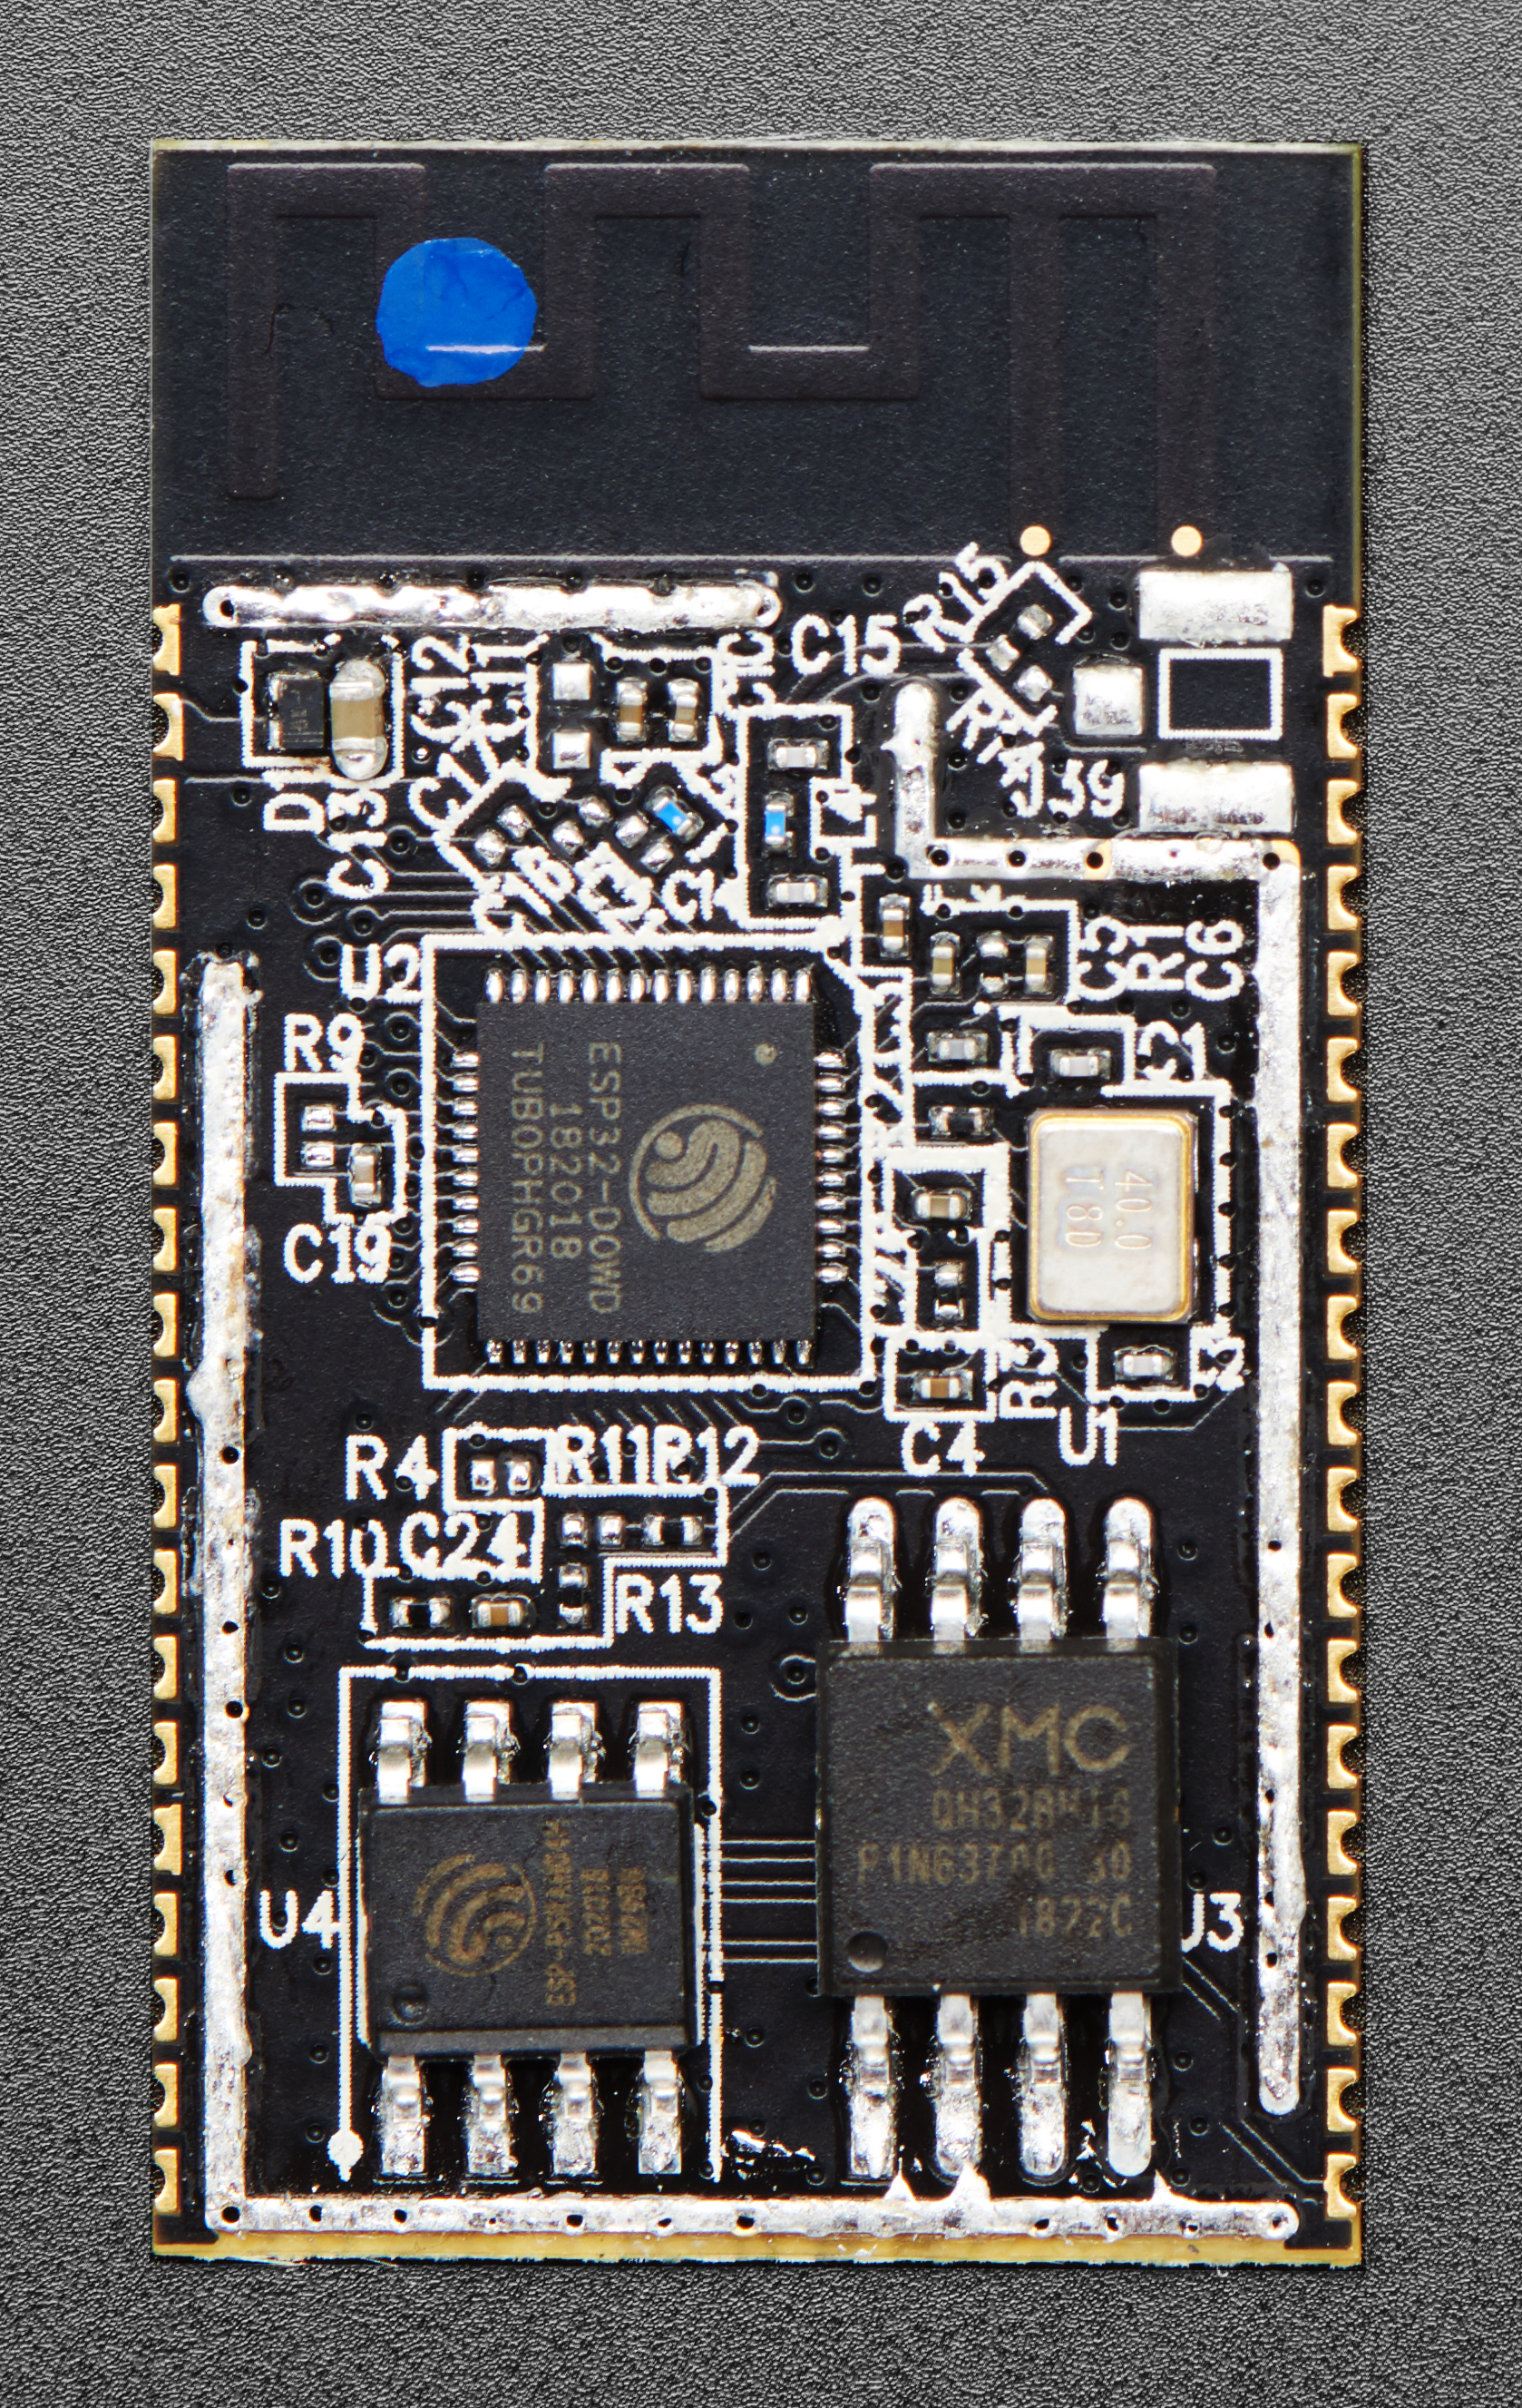
\includegraphics[width=.85\linewidth]{media/esp32_wrover_b.png}
            \subcaption{Фото модуля ESP32-WROVER-B на базе чипа ESP32 \parenciteit{}{ESP32_WROVER_B:Image}}
            \label{fig:ESP32_WROVER_B}
        \end{minipage}
        \hspace{.04\linewidth}
        \begin{minipage}[H]{.5\linewidth}
            \centering
            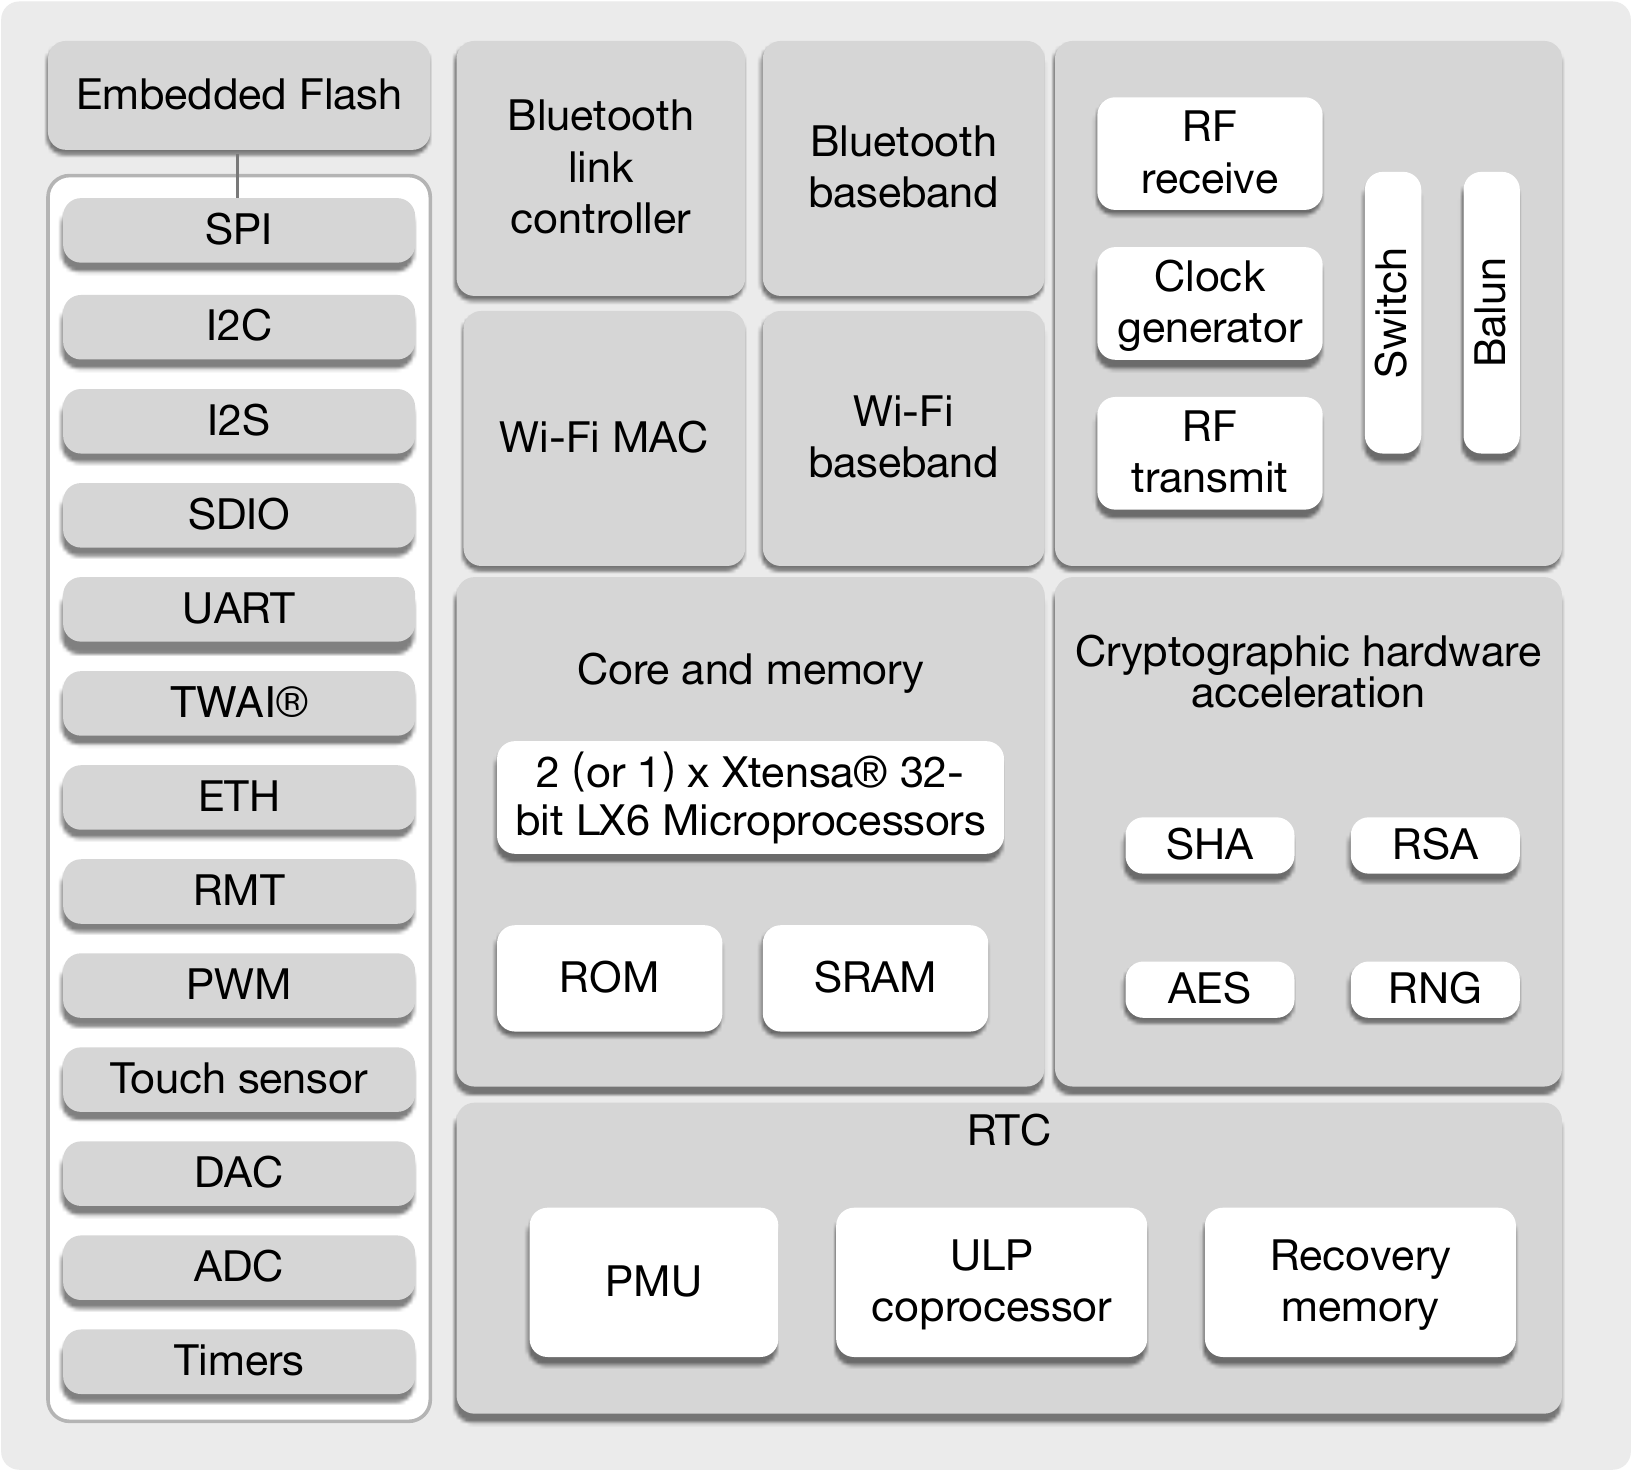
\includegraphics[width=\linewidth]{media/esp32_block_diagram.png}
            \subcaption{Структурная схема типового чипа линейки ESP32 \parenciteit{p12}{ESP32:Datasheet}}
            \label{fig:ESP32_BD}
        \end{minipage}
        \caption{}
        \label{fig:ESP32}
    \end{figure}

    \begin{figure}[!htb]
        \centering
        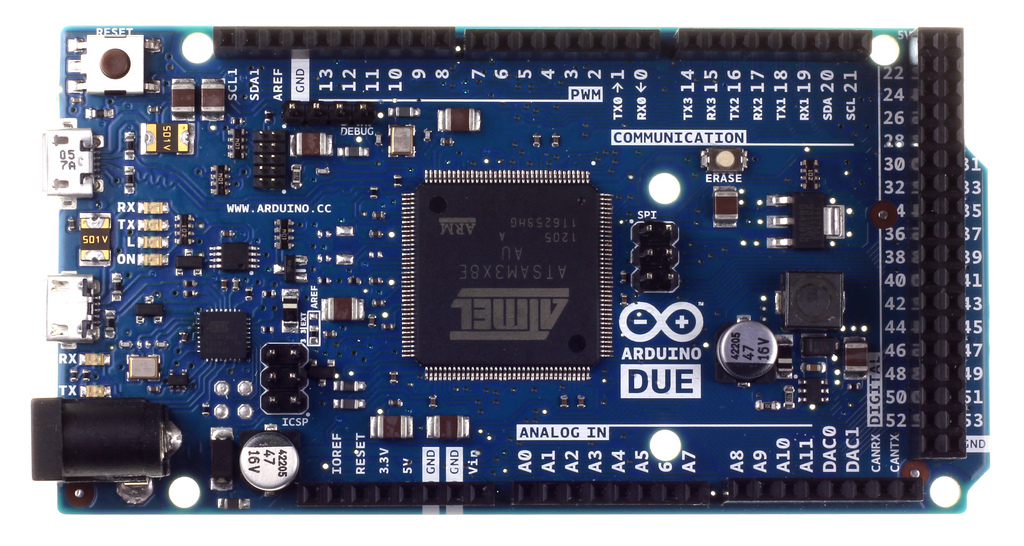
\includegraphics[width=.7\linewidth]{media/ArduinoDue_Front.jpg}
        \caption{Плата Arduino Due \parenciteit{}{ArduinoDue:Image}}
        \label{fig:ArduinoDue}
    \end{figure}
    \clearpage
    \todo{найти все ссылки ??}
    \subsubsection{Питание}\label{sec:MotherboardDesignSupply}
    Питание схемы --- одна из незаменимых и важных частей для её правильной работы, особенно когда присутствуют аналоговые схемы.
    В моём случае питание должно иметь постоянное во времени напряжение и относительно низкий уровень шумов\footnote{Напряжение должно быть постоянным и свободным от помех во всех возможных режимах работы схемы (то есть при разном потреблении тока)}.
    Следовательно, мне нужно выбрать топологию, которая вносила бы минимальные помехи при преобразовании напряжения и которую я мог бы применить как в текущей, так и в будущих версиях прототипа.
    Лучший способ для этого --- использовать линейный стабилизатор, работающий по резистивному принципу.
    Причина его точности в том, что для снижения напряжения до нужного уровня он рассеивает необходимую разницу в виде тепла: это эффект клиппинга, применённый к шуму источника\footnote{Имеется в виду питание стабилизатора}, ценой собственного КПД.

    Напряжение источников, которое к тому же стараются не менять, должно быть таким, чтобы его можно было стабилизировать несложной и эффективной системой с питанием от аккумулятора\footnote{Имеются в виду Li-po аккумуляторы, минимальное напряжение которых (без переразряда) составляет $3.6V$}, чтобы АЦП мог обмениваться данными на том же логическом уровне напряжения\footnote{Напряжение, при котором работают логические интерфейсы чипа}, что и ESP32, то есть $3.3V$, и чтобы питать сам ESP32.
    Картина с использованием $3.3V$ идеально дополняется решением для окончательного прототипа: сочетанием понижающего (buck)\footnote{Схема, понижающая напряжение за счёт свойств индуктивности (с возможностью гальванической развязки) с высоким КПД, ценой вносимого в систему высокочастотного шума, который растёт с увеличением потребляемого тока} преобразователя, чтобы сделать эффективным\footnote{}\todo{<-- добавить ссылку про КПД} преобразование напряжения с $4.2V-3.6V$ примерно до\footnote{Это значение придётся уточнить при проектировании источника питания окончательного прототипа с учётом характеристик выбранных компонентов} $3.5V$, и подключённых за ним линейных стабилизаторов, чтобы убрать шум, внесённый предыдущим каскадом\todo{<-- добавить ссылку про надёжность}, и обеспечить нужные $3.3V$.
    Это решение приводит к тому, что для прототипа можно использовать исключительно линейные стабилизаторы, чтобы смоделировать\footnote{Благодаря эффекту клиппинга линейных стабилизаторов мы, как правило, не замечаем шумов, внесённых в питание предыдущими каскадами (разумеется, если шум не опускается ниже предела, называемого «dropout», за которым линейные стабилизаторы перестают поддерживать постоянное напряжение): следовательно, эти каскады можно опустить} окончательную ситуацию проекта и уменьшить сложность используемых схем.

    В конкретном случае прототипа положительный источник постоянного напряжения уже имеется\footnote{Стабилизация линейная, резистивного типа} на Arduino DUE, которая питается от USB-кабеля $5V$, когда плата подключена к компьютеру для необходимого обмена данными через последовательный порт.
    Отрицательный источник, который понадобится для фильтров\footnote{Причины рассматриваются в разделе\ref{sec:SensorBoardSchematic}}\todo{добавить, что при отфильтровывании постоянной составляющей сигнал получает отрицательную часть}, получается от трансформатора\footnote{Рисунок \ref{fig:ProtoSupplyPhoto}} на $\Delta U = 12V$ без соединения с \texttt{GND}\footnote{Имеется в виду проводник с опорным потенциалом $0V$} розетки, с гальванической развязкой от сети, чтобы его можно было правильно подключить, не вызывая коротких замыканий.
    Затем напряжение понижается до $3.3V$ линейным резистивным стабилизатором.
    Это позволяет мне получить два источника напряжения $3.3V$ и $-3.3$, соединив источники последовательно с \texttt{GND} схемы в точке их соединения, как показано на рисунке \ref{fig:ProtoSupplyConnection}.
    \begin{figure}[H]
        \centering
        \begin{minipage}{.44\linewidth}
            \centering
            \begin{tikzpicture}[transform shape, use fpu reciprocal]
                \draw (0,0)
                    node[above]{$U_{+}$}
                    to[short, o-] ++(0,0)
                    ++(0,-2)
                    to[V=$5V$, l_=$V_1$] ++(0,2)
                    ++(0,-2)
                    coordinate(joint)
                    to[short, -o] ++(1,0)
                    node[right]{$U_{GND}$}
                    (joint) 
                    ++(0,-2)
                    to[V=$12V$, -*, l_=$V_2$] ++(0,2)
                    ++(0,-2)
                    to[short, o-] ++(0,0)
                    node[below]{$U_{-}$};
            \end{tikzpicture}
            \subcaption{Источники $V_1$ и $V_2$ соединены последовательно с \texttt{GND} посередине, чтобы обеспечить $\Delta U_{GND\rightarrow +}=5V$ $\Delta U_{GND\rightarrow -}=-12V$}
            \label{fig:ProtoSupplyConnection}
        \end{minipage}
        \hspace{.04\linewidth}
        \begin{minipage}[H]{.44\linewidth}
            \centering
            % [2026 revision] replaced 4608x2229 prototype-era snapshot with a clean photo of the
            % 12V charger (was: media/album/PSX_20220227_234319.jpg — kept on disk unchanged)
            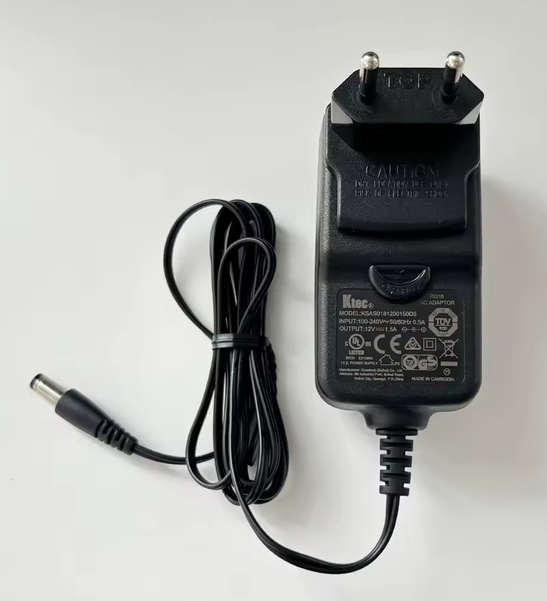
\includegraphics[width=\linewidth]{media/album/12v-charger.jpg}
            \subcaption{Блок питания, которым я преобразую напряжение сети в $12V$, с максимальным током $500mA$}
            \label{fig:ProtoSupplyPhoto}
        \end{minipage}
        \caption{}
        \label{fig:ProtoSuppy}
    \end{figure}
    \clearpage

    \noindent Схема, с помощью которой я понижаю напряжение с $12V$ до $3.3V$, показана на следующем рисунке:
    \begin{figure}[H]
        \centering
        \begin{minipage}[H]{.44\linewidth}
        \centering
        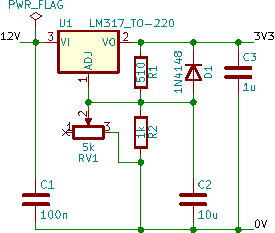
\includegraphics[page=1, width=\linewidth]{media/power_source_board_pcb_cropped.pdf}
        \subcaption{Принципиальная схема, составленная в программе KiCad \parenciteit{}{KiCad:Software}, где выходное напряжение регулируется потенциометром $RV1$ \emph{(Схема спроектирована с расчётом на повторное использование в будущих прототипах, поэтому в ней есть блокировочные конденсаторы $C1$ \& $C3$, о которых я говорю в разделе \ref{sec:SensorBoardSchematic}, и диод $D1$ с конденсатором $C2$ для защиты от коротких замыканий)} \emph{(Частично взято из \cite[p9]{LM317:Datasheet})}}
        \label{fig:PowerSourceBoardSchematic}
        \end{minipage}
        \hspace{.04\linewidth}
        \begin{minipage}[H]{.45\linewidth}
            \centering
            \begin{minipage}[H]{\linewidth}
                \centering
                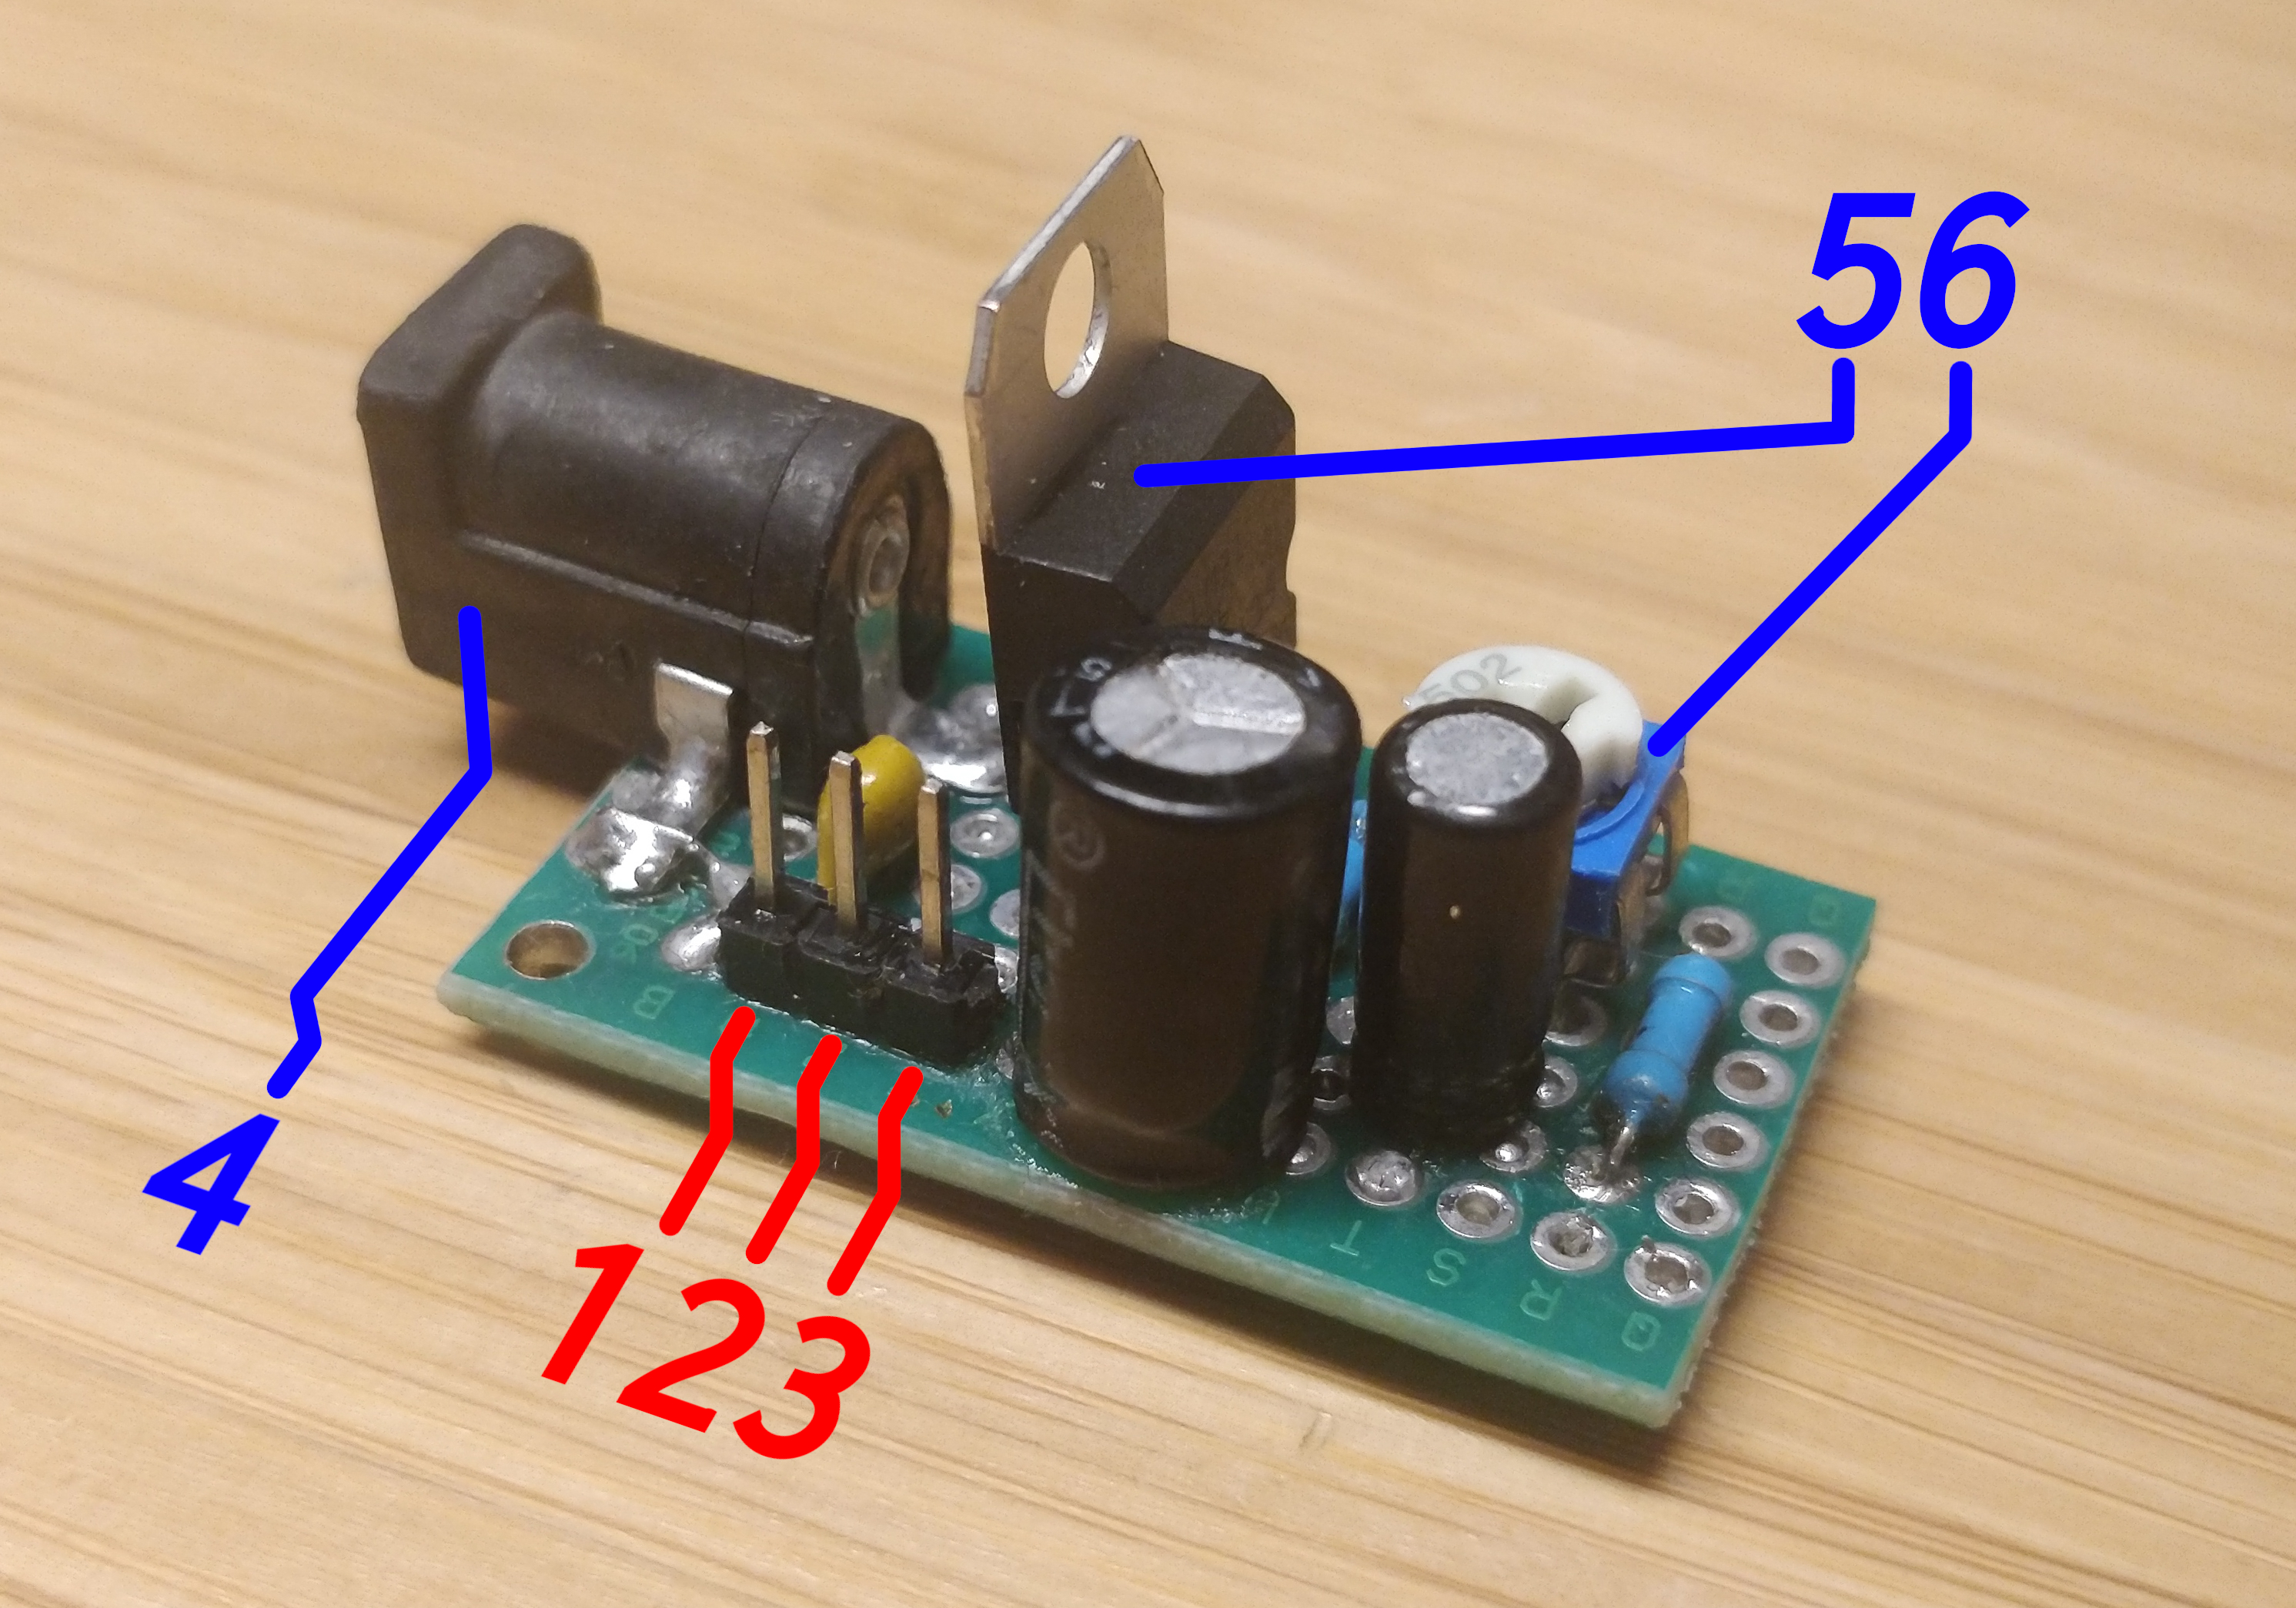
\includegraphics[width=.66\linewidth]{media/album/PSX_20220227_234533_ed.jpg}
                \subcaption{Плата стабилизатора и её компоненты. Красным: $1$ --- вывод $0V$, $2$ --- вывод $12V$, $3$ --- вывод $3V3$. Синим: $4$ --- разъём блока питания, $5$ --- LM317, $6$ --- потенциометр $RV1$ \emph{(На момент сборки у меня не было керамического конденсатора $C3$, и я заменил его электролитическим)}}
                \label{fig:PowerSourceBoardPhoto}
            \end{minipage}
            \\
            \begin{minipage}[H]{\linewidth}
                \centering
                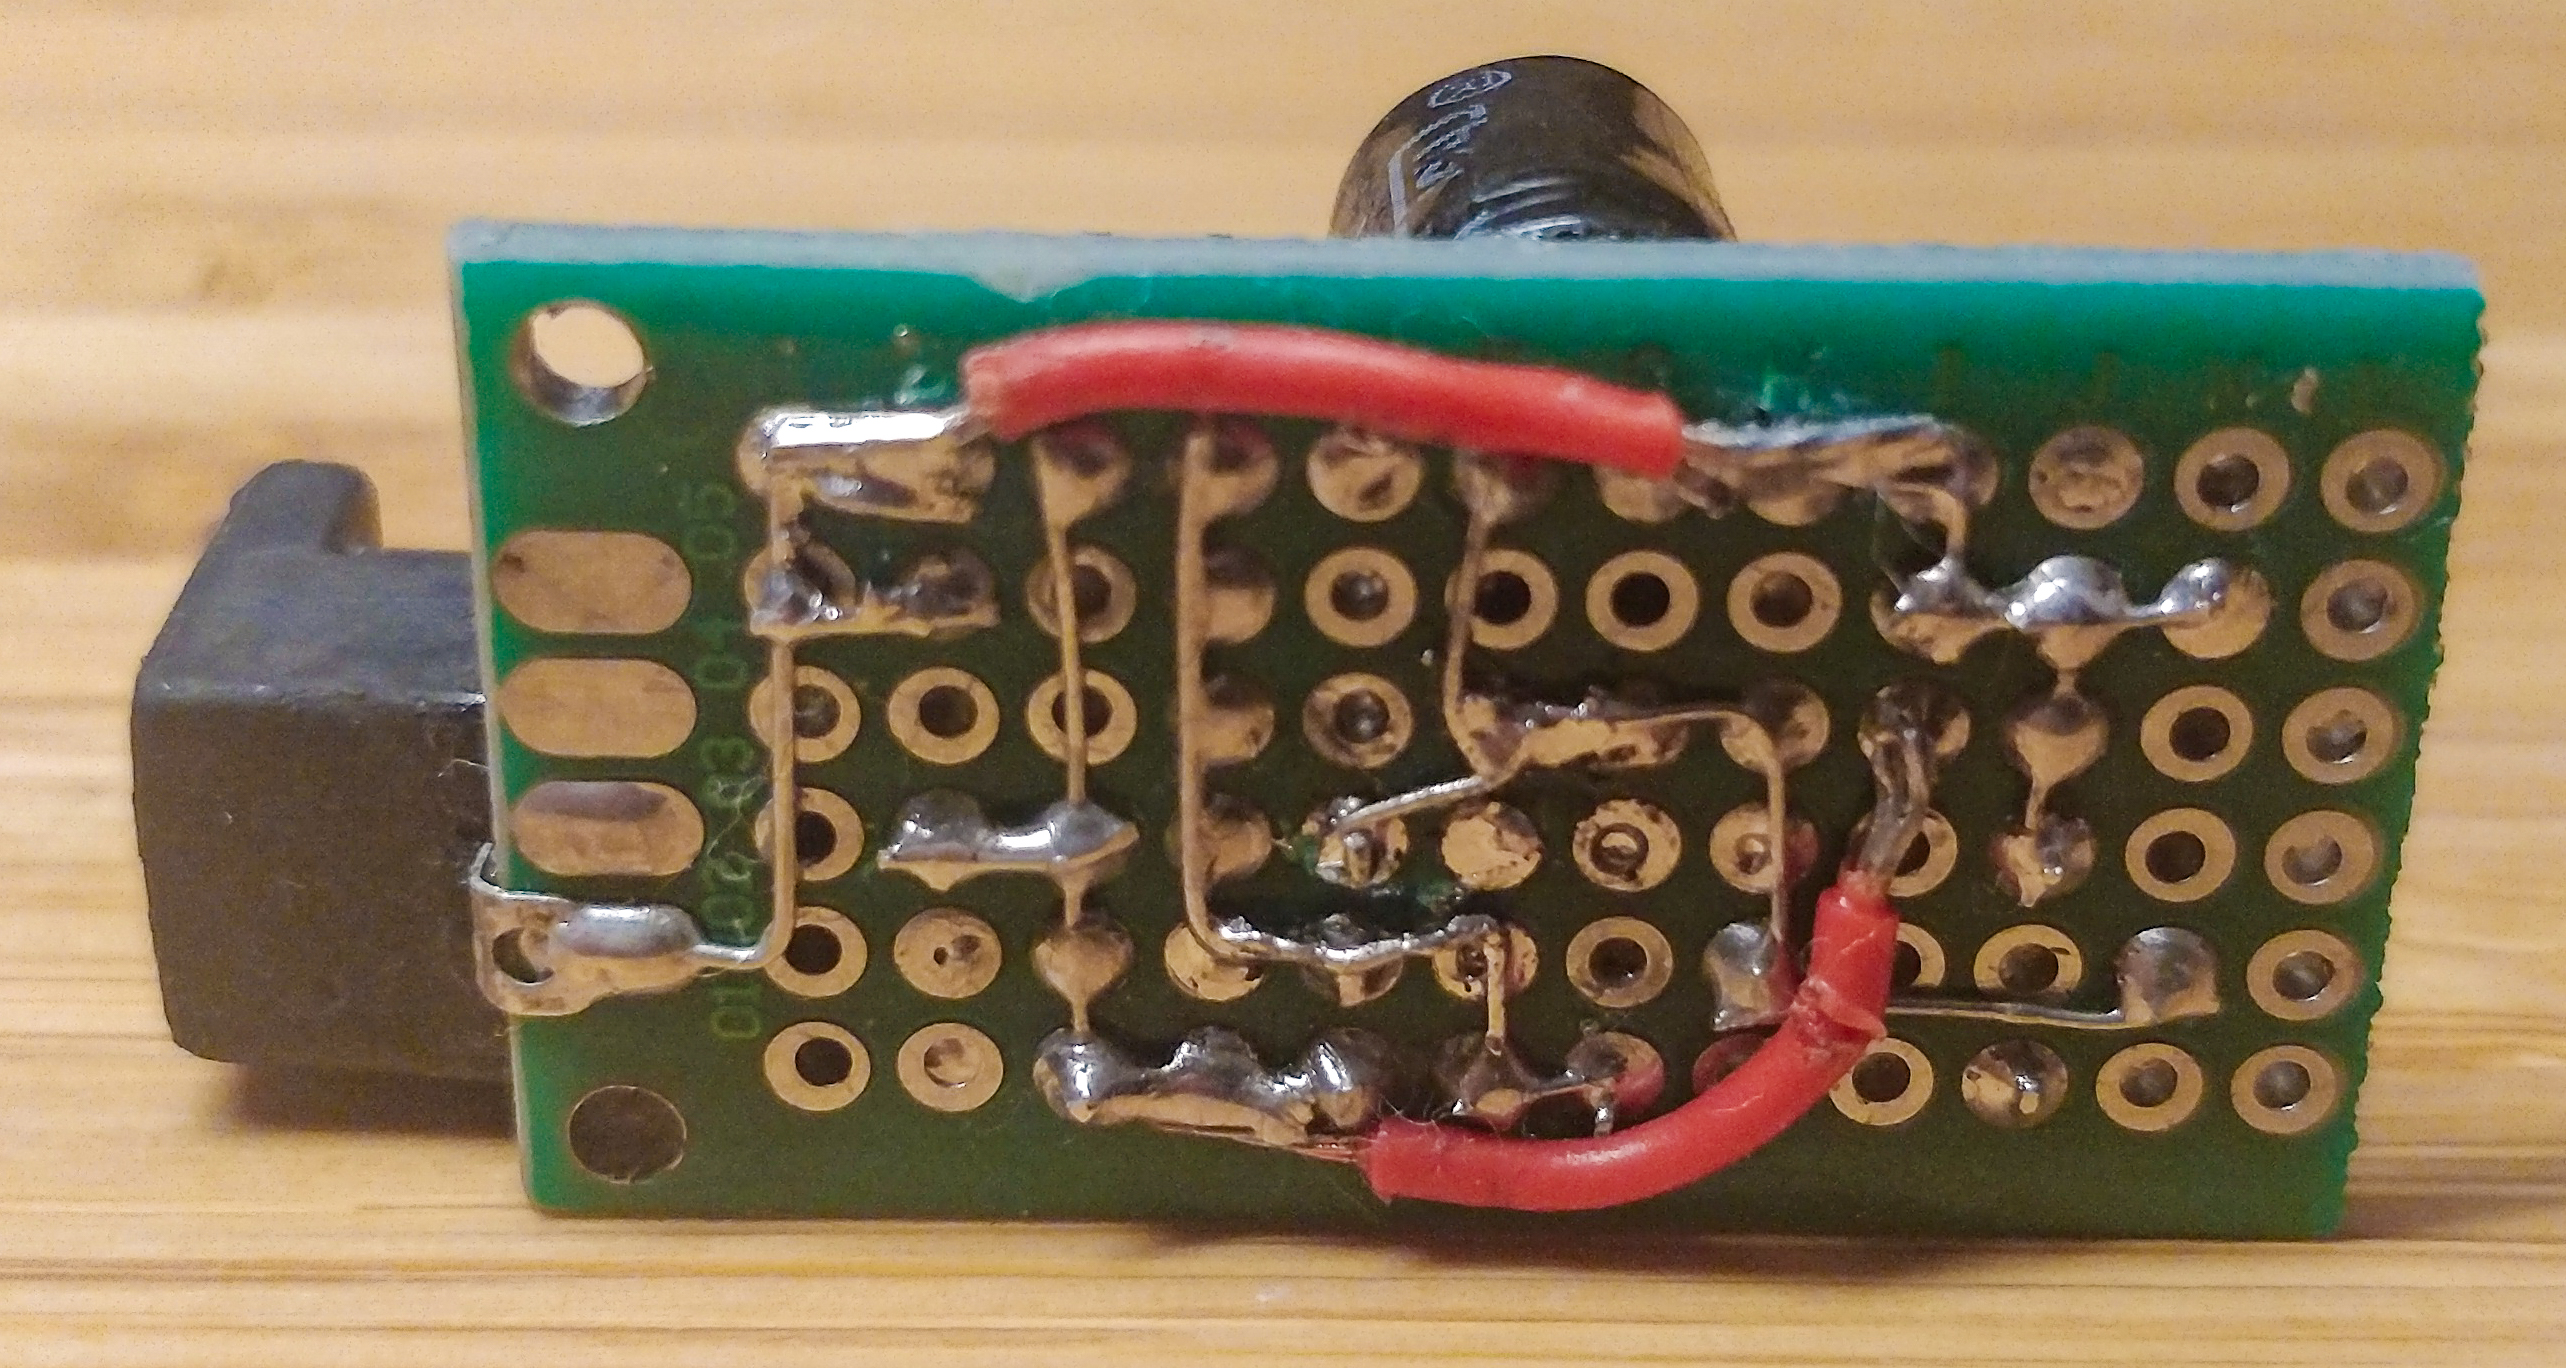
\includegraphics[width=.8\linewidth]{media/album/PSX_20220227_234420.jpg}
                \subcaption{Соединения компонентов на обратной стороне платы стабилизатора: схема собрана по технологии THT \emph{(Through Hole Technology, монтаж в отверстия)}, чтобы сократить время на проектирование и сборку}
                \label{fig:PowerSourceBoardPhotoBack}
            \end{minipage}
        \end{minipage}
        \caption{Плата регулируемого линейного стабилизатора ($1.25V-3.375V$) на базе LM317 \parenciteit{}{LM317:Datasheet}}
        \label{fig:PowerSourceBoard}
    \end{figure}
    \todo{добавить ссылку на GitHub проекта}
    \noindent Расчёты, необходимые для определения сопротивлений, следующие:
    
    \begin{figure}[H]
        \centering
        \begin{minipage}[H]{.15\linewidth}
            \[U_{out} \approx 3.3V\]
        \end{minipage}
        \begin{minipage}[H]{.15\linewidth}
            \[U_{ref}=1.25V\]
        \end{minipage}
        \begin{minipage}[H]{.15\linewidth}
            \[R_2=1k\Omega\]
        \end{minipage}
        \begin{minipage}[H]{.15\linewidth}
            \[RV_1=5k\Omega\]
        \end{minipage}
        \begin{minipage}[H]{.15\linewidth}
            \[I_{adj}=100\mu A\]
        \end{minipage}
        \begin{minipage}[H]{\linewidth}
            \vspace{3ex}
            \[U_{out}=U_{ref}\left(1+\frac{RV_1 \parallel R_2}{R_1}\right)+I_{adj} \left(RV_1 \parallel R_2\right)\]
        \end{minipage}
    \end{figure} \todo{добавить ссылку на то, как сделать знак параллельного соединения в схеме}
    \noindent $I_{adj}$ --- ток, протекающий через вывод \texttt{ADJ} стабилизатора LM317; как видно, он влияет на $U_{out}$, но при сбалансированном выборе сопротивлений его влияние, как правило, невелико.
    Номиналы резисторов следует выбирать по стандартизированным рядам E\footnote{Эти ряды применяются не только к резисторам, но и к конденсаторам}\:\footcite[]{ESeries:Wiki}.
    После небольшого поиска среди компонентов, которые у меня уже были, и нескольких попыток с расчётами я пришёл к значениям\footnote{Номиналы конденсаторов взяты непосредственно из исходника схемы на рисунке \ref{fig:PowerSourceBoardSchematic}}, которые видны на принципиальной схеме на рисунке \ref{fig:PowerSourceBoardSchematic}.
    \clearpage

    \section{Фильтры --- теория}\label{sec:FilterTheory}
    Под термином «фильтры», учитывая также содержание раздела \ref{sec:SensorboardDesignInput} и раздела \ref{sec:SensorboardDesignOutput}, понимаются частотные фильтры, которые, что удобно\footnote{Причина обсуждается в разделе \ref{sec:ElectronicsCalculusLaplace}}, относятся к LTI-системам\footnote{Термин и его значение обсуждаются в следующем разделе, разделе \ref{sec:FilterTheorySystems}}.

    \subsection{Системы}\label{sec:FilterTheorySystems}
    Когда я упоминаю \emph{Input} и \emph{Output}, я имею в виду понятие системы из теории систем и управления\footcite[]{ControlTheory:Wiki}.
    Эта теория полезна в нашем случае тем, что даёт модель, с помощью которой можно спроектировать систему\footnote{Система изначально --- это абстрактное понятие объекта, который обрабатывает входы и выдаёт выходы и который затем можно реализовать}, позволяющую оптимальнейшим образом достигать желаемых состояний некоторого числа \emph{Output} через состояния некоторого числа \emph{Input}.

    \begin{samepage}
        \noindent Существуют разные категории систем, определяемые их характеристиками, но нас интересует только одна конкретная, к которой относится наш фильтр:
        \begin{enumerate}[label=\emph{(\arabic*)}]
            \item Тип интерфейса: SISO, то есть Single Input Single Output\footnote{Один вход, один выход}
            \item Тип системы: LTI, то есть Linear Time Invariant\footnote{Линейная, инвариантная во времени}
        \end{enumerate}
    \end{samepage}
    Название первой характеристики говорит само за себя, а вторая может показаться менее понятной.
    Два понятия, которые объединяет LTI, --- линейность и инвариантность во времени --- необходимо обсудить.

    Свойство линейности само по себе может проявляться в различных системах, если они не используются на физическом пределе, на который рассчитаны, хотя в основном системы в реальном мире, как правило, нелинейны\footcite[]{TransferFunction:Wiki}.
    \begin{samepage}
        \noindent Конкретно понятие линейности описывается выполнением двух условий:
        \begin{enumerate}[label=\emph{(\arabic*)}]
            \item Аддитивность, описываемая формулой: \[f(x + y) = f(x) + f(y)\]
            \item Однородность, описываемая формулой: \[f(a \cdot x) = a \cdot f(x)\]
        \end{enumerate}
    \end{samepage}

    Реальным примером линейной системы может служить схема, как на рисунке \ref{fig:ExampleLTICircuit}, содержащая транзистор\footnote{В примере рассматривается MOSFET}, \emph{Output} которой будет вести себя линейно\footnote{Это видно на рисунке \ref{fig:ExampleLTIIRFZ44N_Plot_Vgs}} при изменении напряжения\footnote{Это явление наблюдается у MOSFET, но не все транзисторы работают одинаково} на \emph{Input}, если транзистор работает в режиме насыщения.
    % TRANSLATOR NOTE: the inline-math subscript $V_{DS_{saturazione}}$ (also next line) is Italian but left untouched per the math-mode rule; consider $V_{DS_{\mathrm{sat}}}$ or $V_{DS_{\text{нас}}}$.
    Режим насыщения, который можно определить на рисунке \ref{fig:ExampleLTIIRFZ44N_Plot_Vds}, --- это диапазон напряжений $U_{out}$ (соответствующего $V_{DS}$) при $V_{DS_{saturazione}} < V_{DS}$, в котором транзистор ведёт себя линейно при изменении напряжения $U_{in}$\footnote{Его тоже нужно учитывать, так как это параметр функции, показанной на графике: при увеличении $V_{GS}$ растёт напряжение $V_{DS_{saturazione}}$} (соответствующего $V_{GS}$).
    Если же схема работает в триодном режиме, то есть в диапазоне $V_{DS}$ при $0 < V_{DS} < V_{DS_{saturazione}}$, ток $I_D$ начинает зависеть и от $V_{DS}$, то есть от $U_{out}$: при таком поведении схема нарушает два условия, определяющих линейное поведение, и тем самым становится нелинейной системой.
    \begin{figure}[H]
        \centering
        \begin{minipage}{.84\linewidth}
            \centering
            \begin{tikzpicture}[transform shape, use fpu reciprocal]
                \draw (0,0)
                    node[above]{$U_{+}$}
                    to[short, o-] ++(0,-.25)
                    to[R, l=$R$, -*] ++(0,-2)
                    coordinate(joint)
                    to[short, -o] ++(1,0)
                    node[right]{$U_{out}$}
                    (joint) to[short] ++ (0,-.5)
                    node[nigfete, anchor=D, bodydiode, tr circle] (fet) {$Q$}
                    (fet.S) node[anchor=south east] {\footnotesize{\texttt{S}}}
                    (fet.D) node[anchor=north east] {\footnotesize{\texttt{D}}}
                    (fet.G) node[anchor=south west] {\footnotesize{\texttt{G}}}
                    (fet.S) node[ground]{} ++(0,-.5)
                    (fet.G) to[short, -o] ++(-.5,0)
                    node[left]{$U_{in}$};
            \end{tikzpicture}
            \subcaption{IRFZ44N обозначен $Q$ \emph{(}\texttt{G}\emph{ = Gate, }\texttt{D}\emph{ = Drain, }\texttt{S}\emph{ = Source)}, идеальный резистор $R$, источник постоянного напряжения $U_{+}$, \emph{Input} $U_{in}$ и \emph{Output} $U_{out}$}
            \label{fig:ExampleLTICircuit}
        \end{minipage}
        \\
        \vspace{3ex}
        \begin{minipage}[t]{.4\linewidth}
            \centering
            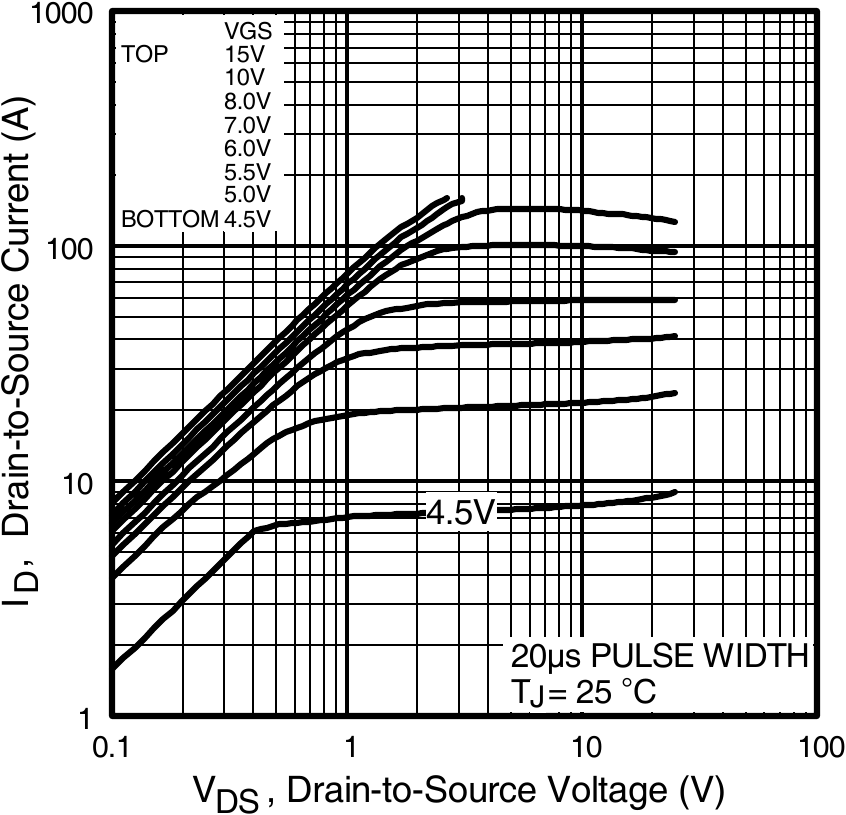
\includegraphics[width=\linewidth]{media/irfz44n_vds_id_plot.png}
            \subcaption{Зависимость $I_D$ от $V_{DS}$ при параметре $V_{GS}$ \emph{(режим насыщения определяется для $V_{DS}$ после того, как рост $I_D$ приблизительно прекращается)}}
            \label{fig:ExampleLTIIRFZ44N_Plot_Vds}
        \end{minipage}
        \hspace{.04\linewidth}
        \begin{minipage}[t]{.4\linewidth}
            \centering
            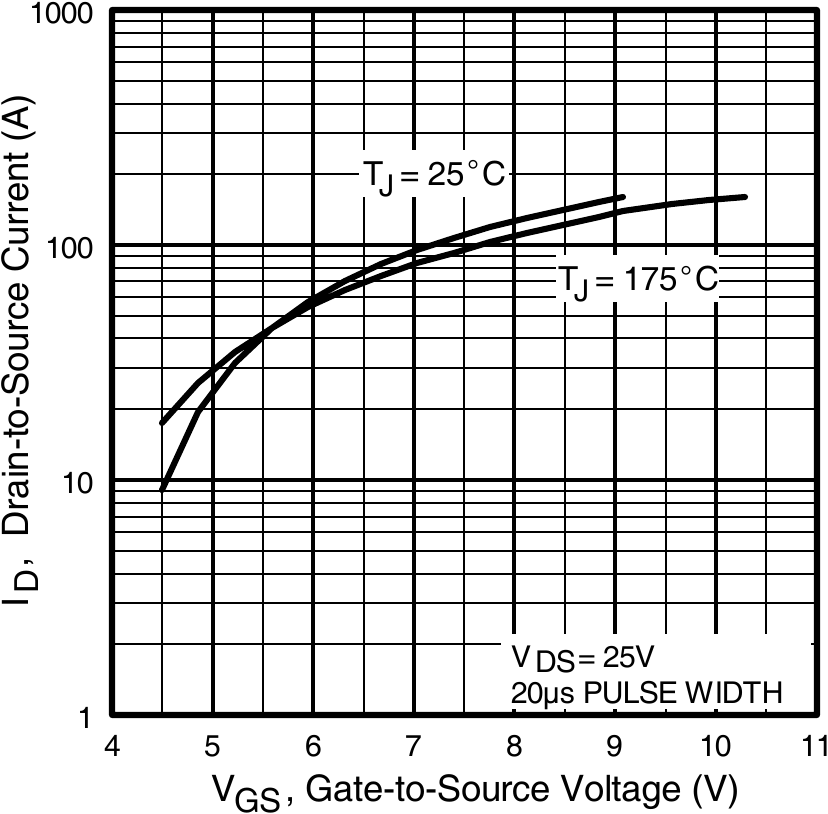
\includegraphics[width=\linewidth]{media/irfz44n_vgs_id_plot.png}
            \subcaption{Зависимость $I_D$ от $V_{GS}$ в режиме насыщения при \emph{($V_{DS} = 25V$)}, приблизительно линейная}
            \label{fig:ExampleLTIIRFZ44N_Plot_Vgs}
        \end{minipage}
        \caption{Пример усилителя на основе IRFZ44N \emph{(транзистор, точнее N-канальный MOSFET с индуцированным каналом)} \parenciteit{}{IRFZ44N:Datasheet} с соответствующей схемой на \ref{fig:ExampleLTICircuit} и графиками \parenciteit{}{IRFZ44N:Datasheet} вольт-амперных характеристик на \ref{fig:ExampleLTIIRFZ44N_Plot_Vds}, \ref{fig:ExampleLTIIRFZ44N_Plot_Vgs}}
        \label{fig:ExampleLTI}
    \end{figure}


    Понятие инвариантности во времени определяется постоянством результатов системы во времени: чтобы считаться инвариантной во времени, система не должна давать разные \emph{Output} при одинаковых \emph{Input} в разные моменты времени.

    Хорошим примером системы, изменяющейся во времени, может служить сайт, показывающий часовые пояса в реальном времени.
    Если запросить дату и время в определённом часовом поясе, каждый раз полученные значения будут отличаться от тех, что будут получены в следующий момент.


    Аналоговый частотный фильтр, который нам нужен, считается LTI-системой потому, что аналоговые схемы, как правило, легко описывают определённые инвариантные во времени системы\footnote{Изменчивость во времени электронной системы, спроектированной как инвариантная, как и её линейность, может зависеть от физических явлений, таких как изменение сопротивления при разных температурах, или от EMI} и линейны по своему отклику, если не используются за пределами расчётных параметров, как напряжение насыщения MOSFET в предыдущем примере.
    Дополнительно отмечу, что изменчивость во времени может иметь смысл с точки зрения обработки сигналов при использовании цифровых систем, где данные не привязаны жёстко ко времени, а дискретны.

    Настоящее преимущество отнесения фильтра к LTI-системам становится заметно, когда понимаешь их свойства\footnote{Свойства и связи между ними обсуждаются в разделе \ref{sec:TransformsAndLaplace}}: возможность описать систему откликом на импульс и прямое следствие этого факта --- возможность представить систему функцией, называемой передаточной функцией.
    \clearpage

    \subsection{Математика \& физика} \label{sec:MathAndPhysics}
    Я уже упоминал передаточные функции\footcite[]{TransferFunction:Wiki} в предыдущих разделах\footnote{Раздел \ref{sec:IntroFiltersSignals} и раздел \ref{sec:FilterTheorySystems}} и их свойство быть абстракцией фильтра.
    \begin{samepage}
        Нужно учитывать следующие равенства:
        \begin{figure}[H]
            \centering
            \begin{minipage}[b]{.35\linewidth}
                \centering
                \[
                    H(s) = \frac{Output}{Input} = \frac{U_{out}}{U_{in}}
                \]
            \end{minipage}
            \begin{minipage}[b]{.35\linewidth}
                \centering
                \[
                    s = j\omega\ + \sigma
                \]
            \end{minipage}
        \end{figure}
    \end{samepage}

    Передаточные функции, обычно обозначаемые заглавной буквой $H(s)$ в нотации математической функции, --- это функции, описывающие связь области определения, то есть \emph{Input}, и области значений, то есть \emph{Output}, как функцию комплексной переменной $s$, связывая \emph{Input} и \emph{Output} путём деления одного на другое.
    Кроме того, зная, что изучаемый сигнал описывается изменениями напряжения, сопоставим \emph{Input} с $U_{in}$, а \emph{Output} --- с $U_{out}$.

    Из физики и математики мы знаем, что $j$, которое в нашем случае обозначает мнимую единицу \(i\), умножается на $\omega$, образуя тем самым мнимую часть $s$ при условии $\Im(\omega) = 0$.
    \(\sigma\), напротив, образует действительную часть \(s\), опять же при аналогичном условии $\Im(\sigma) = 0$.

    \noindent Передаточную функцию можно описать также двумя многочленами: $N_n(x)$ в числителе и $D_m(y)$ в знаменателе, следующим образом:
    \begin{figure}[H]
        \centering
        \begin{minipage}[b]{.3\linewidth}
            \centering
            \[
                N_n(x) = \sum^{n}_{k=0} a_k x^k \mathrm{,}
            \]
        \end{minipage}
        \begin{minipage}[b]{.3\linewidth}
            \centering
            \[
                D_m(y) = \sum^{m}_{j=0} b_j y^j \mathrm{,}
            \]
        \end{minipage}
        \begin{minipage}[b]{.3\linewidth}
            \centering
            \[
                H(s) = \frac{N_n(s)}{D_m(s)}
            \]
        \end{minipage}
    \end{figure}
    \noindent Тогда $H(s)$ можно переписать через многочлены в развёрнутой или разложенной на множители форме
    \begin{figure}[H]
        \centering
        \begin{minipage}[b]{.45\linewidth}
            \centering
            \[
                H(s) = \frac{a_0 + a_1 s + \dotsm + a_{n-1} s^{n-1} + a_n s^n}{b_0 + b_1 s + \dotsm + b_{m-1} s^{m-1} + b_m s^m} \mathrm{,}
            \]
        \end{minipage}
        \hspace{0.04\linewidth}
        \begin{minipage}[b]{.45\linewidth}
            \centering
            \[
                H(s) = \frac{z_0 \left(s - z_1\right) \dotsm \left(s^{n-1} - z_{n-1}\right) \left(s^n - z_n\right)}{p_0 \left(s - p_1\right) \dotsm \left(s^{m-1} - p_{m-1}\right) \left(s^m - p_m\right)}
            \]
        \end{minipage}
    \end{figure}
    \noindent и, подставив в равенство выражение $K = \frac{z_0}{p_0}$, соответствующее коэффициенту усиления\footnote{Эта переменная понадобится нам позже} \todo{Пересмотреть сноску на предмет ссылок}
    \begin{figure}[H]
        \centering
        \[
            H(s) = K \frac{\left(s - z_1\right) \left(s^2 - z_2\right) \dotsm \left(s^{n-1} - z_{n-1}\right) \left(s^n - z_n\right)}{\left(s - p_1\right) \left(s^2 - p_2\right) \dotsm \left(s^{m-1} - p_{m-1}\right) \left(s^m - p_m\right)}
        \]
    \end{figure}
    \noindent Из равенств следует:
    \begin{figure}[H]
        \centering
        \begin{minipage}[b]{.3\linewidth}
            \centering
            \[
                \lim_{s \to z_i} H(s) = 0
            \]
        \end{minipage}
        \hspace{0.04\linewidth}
        \begin{minipage}[b]{.3\linewidth}
            \centering
            \[
                \lim_{s \to p_i} H(s) = \infty
            \]
        \end{minipage}
    \end{figure}
    % TRANSLATOR NOTE: original calls poles "picchi" (peaks); translated with the standard term "полюсы".
    \noindent Для любого $s$, стремящегося к значениям $z_i$, логично названным «\emph{нулями}», значение функции $H(s)$ стремится к $0$, а когда $s$ стремится к $p_i$, не менее логично названным «\emph{полюсами}», $H(s)$ становится $\infty$.
    С этого момента передаточные функции можно описывать только \emph{нулями}, \emph{полюсами} и $K$ --- коэффициентом усиления.

    Характеристика передаточной функции, которая пригодится нам \todo{Добавить ссылку на порядок фильтров} в физической части, --- это порядок передаточной функции.
    % TRANSLATOR NOTE: display-math line below read "ordine = m"; changed to \text{порядок} = m (Cyrillic cannot appear raw in math mode). Only math-mode edit in the file.
    Порядок определяется числом полюсов функции:
    \[
        \text{порядок} = m
    \]

    Чтобы понять, какие изменения вносятся во \emph{Input} функции, комплексное число $s$ можно изобразить на плоскости с $\omega$ на действительной оси и $\sigma$ на мнимой оси, построив так называемый «\emph{s-plot}»\footnote{Рисунок \ref{fig:ExampleSPlot}}, на котором \emph{полюсы} можно отметить крестиками, а \emph{нули} --- кружками.

    \begin{figure}[!htb]
        \centering
        \hspace{0.15\textwidth}
        \begin{tikzpicture}
            \begin{axis}[
                axis x line=middle,
                axis y line=middle,
                xlabel={$\sigma$},
                ylabel={$\omega$},
                legend entries={$\lim_{s \to p_i} H(s)$, $\lim_{s \to z_i} H(s)$},
                legend pos=north east,
                height=.4\textwidth,
                width=.4\textwidth,
                clip=true,
                xtick distance=.5,
                ytick distance=.5,
                xmin=-1.25,
                xmax=1.25,
                ymin=-1.25,
                ymax=1.25,
                ymajorgrids=true,
                xmajorgrids=true,
                grid style=dashed,
                axis_style_default
            ]
            \addplot[
                only marks,
                color=blue!75,
                mark size=.75ex,
                thick,
                mark=x
            ]
                coordinates{(-0.707,0.707)(-0.707,-0.707)};
            \addplot[
                only marks,
                color=blue,
                mark size=.75ex,
                thick,
                mark=o
            ]
                coordinates{(0,0)};
            \end{axis}
        \end{tikzpicture}
        \caption{Пример s-plot для $H(s)$, функции II порядка}
        \label{fig:ExampleSPlot}
    \end{figure}
    
    Продолжая рассуждение, ответим на вопрос, чему соответствует \(\omega\).
    Через \(\omega\) в физике часто обозначают угловую частоту, то есть частоту, измеряемую в \([\frac{rad}{s}]\), а не в \([Hz]\). Связь простая:
    \[ \omega = 2\pi\cdot f\]

    % TRANSLATOR NOTE: "coefficiente di rafforzamento del segnale" (sigma) rendered consistently as "коэффициент нарастания сигнала".
    В то же время \(\sigma\) с физической точки зрения обозначает коэффициент нарастания сигнала, смысл которого гораздо проще понять, если использовать вместо неё \(\zeta\), которая предстаёт как классический коэффициент затухания гармонического колебания.
    \[ \sigma = -\zeta\]

    \begin{samepage}
        \noindent Чтобы лучше понять влияние $\zeta$ на \emph{Input}, предлагаю пример на рисунке \ref{fig:ExampleDampingAndFrequencyDifference}
        \begin{figure}[H]
            \centering
            \begin{tikzpicture}
                \begin{axis}[
                    axis x line=middle,
                    axis y line=middle,
                    xlabel={$x$},
                    ylabel={$y$},
                    legend entries={$(a)$ $\zeta=0.1$, $(b)$ $\zeta=0.2$, $(c)$ $\zeta=0.6$},
                    legend pos=north east,
                    height=.4\textwidth,
                    width=.9\textwidth,
                    clip=true,
                    domain=0*pi:7*pi,
                    x_axis_style_pi=2,
                    ytick distance=0.5,
                    xmin=0,
                    xmax=20,
                    ymin=-1.1,
                    ymax=+1.1,
                    smooth,
                    ymajorgrids=true,
                    xmajorgrids=true,
                    grid style=dashed,
                    axis_style_default
                ]
                \addplot [thick, color=gray!75] {1.00503 * sin(x * 0.99498) * (2.71828 ^(-0.1 * x)) };
                \addplot [thick, color=blue!75] {1.02062 * sin(x * 0.97979) * (2.71828 ^(-0.2 * x)) };
                \addplot [thick, color=red!75]  {1.25    * sin(x * 0.8)     * (2.71828 ^(-0.6 * x)) };
            \end{axis}
            \end{tikzpicture}
            \caption{Пример трёх сигналов системы II порядка с $\omega=1$, полученных как отклик на импульсную функцию $\delta(x)$ \emph{(функция, называемая также «дельта-функцией Дирака», которая при любом $x$ равна $y = 0$, кроме $x = 0$, где $y = +\infty$)} \parenciteit{}{Impulse:Wiki}}
            \label{fig:ExampleDampingAndFrequencyDifference}
        \end{figure}
    \end{samepage}

    Однако по-прежнему неясно, как преобразовать передаточную функцию, заданную как функция значений $s$, в функцию времени $t$, которая описывала бы реакцию на сигнал --- как на импульс, как на рисунке \ref{fig:ExampleDampingAndFrequencyDifference}, так и на любой другой тип сигнала.
    Для этого нужно обратиться сначала к теме преобразований в целом, а затем конкретно к преобразованию Лапласа.

    \begin{samepage}%
        \subsubsection{Преобразования \& Лаплас} \label{sec:TransformsAndLaplace}
        Начнём с определения преобразования\footnote{Называемого также «интегральным преобразованием»}: \nopagebreak
        \begin{figure}[H]
            \Centering
            \vspace{1ex}
            \textit{«Интегральное преобразование отображает функцию из её исходного функционального пространства в другое функциональное пространство посредством интегрирования, где некоторые свойства исходной функции можно охарактеризовать и обработать легче, чем в исходном функциональном пространстве.» }

            \RaggedLeft
            \vspace{1ex}

            \scriptsize{\parenciteit{}{Transform:Wiki}}
            \vspace{1ex}
        \end{figure}
        \noindent Иначе говоря, преобразования служат для смены области определения функций, чтобы с ними было удобнее работать.
    \end{samepage}%

    \begin{samepage}%
        Начнём прежде всего с передаточных функций, то есть «\emph{Input}» преобразований: передаточные функции изначально задаются дифференциальными уравнениями\footnote{Пример я привожу в разделе \ref{sec:ElectronicsCalculusLaplace}}, описывающими поведение выходного сигнала относительно входного во временной области, например:
        \begin{figure}[H]
            \centering
            \begin{minipage}[b]{.3\linewidth}
                \centering
                \[
                    3\frac{\mathrm{d}^2y}{\mathrm{d}t^2} + 2\frac{\mathrm{d}y}{\mathrm{d}t} + 7 = 1 + 5\frac{\mathrm{d}y}{\mathrm{d}t} \mathrm{,}
                \]
            \end{minipage}
            \hspace{0.04\linewidth}
            \begin{minipage}[b]{.3\linewidth}
                \centering
                \[
                    H(s) = \frac{5s + 1}{3s^2 + 2s + 7}
                \]
            \end{minipage}
        \end{figure}
        \noindent Для упрощения такого рода дифференциальных выражений требуется свёртка\footnote{Объясняется далее в этом разделе}\:\footcite[]{Convolution:Wiki} функций, которая при решении без использования свойств вроде свойств преобразования Лапласа может стать очень сложной.
    \end{samepage}%

    \begin{samepage}
        % TRANSLATOR NOTE: original writes "casuali" (random) for "causali"; translated as "причинные" / "непричинные".
        \noindent Преобразование Лапласа определяется следующим\footnote{Существует два вида преобразования: одностороннее, определённое на интервале $\{0,\infty\}$ и используемое для причинных систем, называемых также неупреждающими (выполняется $f(t<0)=0$), и двустороннее, $\{-\infty,\infty\}$, для непричинных систем, называемых упреждающими (результат может появиться раньше, чем поступит вход)}\:\footnote{Я использую определение одностороннего преобразования Лапласа для причинных систем, таких как LTI-системы} образом: \nopagebreak
        \[
            \mathcal{L}\{f\}(s) = \int_{0}^{\infty} f(t) \cdot e^{-st} \mathrm{d}t
        \]
    \end{samepage}%
    \noindent Преобразование Лапласа берёт функцию во временной области и преобразует её в функцию в области $s$, которая, как уже сказано, имеет две составляющие: $\omega$ --- угловую частоту и $\sigma$ --- коэффициент нарастания сигнала.
    \begin{samepage}
        Чтобы лучше почувствовать, что происходит «за кулисами», можно представить преобразование Лапласа как преобразование Фурье, которое, подобно первому\footnote{В преобразовании Фурье $\sigma$ не учитывается, предполагается $\sigma = 0$}, отображает функции с областью определения $t$ в функции с областью определения $\omega$\footnote{Преобразование Фурье даёт разложение рассматриваемой функции по частотам}, но с одним параметром меньше --- без $\sigma$:
        \[
            \mathcal{F}\{f\}(\omega) = \int_{0}^{\infty} f(t) \cdot e^{-j\omega t} \mathrm{d}t
        \]
        \noindent Следовательно, с помощью преобразования Лапласа можно увидеть функции Фурье для разных коэффициентов нарастания.
    \end{samepage}%
    
    Полезность преобразования Лапласа не только в том, что я только что объяснил, но и в другом его свойстве: если в дифференциальных расчётах получается свёртка, то с помощью Лапласа она превращается в умножение\footnote{Это будет показано в разделе \ref{sec:ElectronicsCalculusLaplace}}

    Один из способов понять, откуда берутся свёртки в дифференциальных расчётах систем, --- поразмышлять о связи Input и Output преобразования.
    С помощью обратного\footnote{Просто меняются местами области, между которыми действует преобразование: из $s$ в $t$} преобразования Лапласа $\mathcal{L}^{-1}$ можно получить временной отклик LTI-системы на импульс\footnote{Дельта-функция Дирака, упомянутая на рисунке \ref{fig:ExampleDampingAndFrequencyDifference}}.
    Если взять бесконечную последовательность импульсов \emph{(высотой, соответствующей высоте описываемой функции в интересующий момент)}, можно составить непрерывную функцию.
    Выход системы будет свёрткой\footnote{Как в примере на рисунке \ref{fig:ConvolutionExample}} входного сигнала, то есть функции, которую можно описать импульсами, с откликом системы на дельта-функцию Дирака.
    \begin{figure}[H]
        \centering
        \begin{minipage}[H]{.3\linewidth}
            \centering
            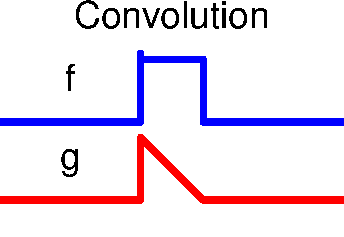
\includegraphics[page=1, width=\linewidth]{media/convolution1.pdf}
        \end{minipage}
        \hspace{.04\linewidth}
        \begin{minipage}[H]{.3\linewidth}
            \centering
            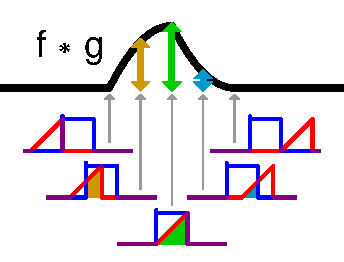
\includegraphics[page=1, width=\linewidth]{media/convolution2.pdf}
        \end{minipage}
        \caption{Пример свёртки двух функций \parenciteit{}{Convolution:Image}}
        \label{fig:ConvolutionExample}
    \end{figure} 
    \noindent Это свойство очень полезно, когда дифференциальные расчёты начинают усложняться. Чтобы лучше разобраться и развить изложение в сторону связи с физикой, попробуем в следующем разделе решить пример из электротехники.
    
    \subsubsection{Электротехника \& дифференциальное исчисление \& Лаплас} \label{sec:ElectronicsCalculusLaplace}
    Рассмотрим схему на следующем рисунке \ref{fig:CapTrasferFunctionExampleSchematic}:
    \begin{figure}[H]
        \centering
        \begin{tikzpicture}[transform shape, use fpu reciprocal]
            \draw (0,-2)
                to[sV=$U$, l_=$V_1$] ++(0,2)
                -- ++(.5,0)
                to[nopb=$SW_1$] ++(2,0)
                to[R, l=$R_1$] ++(2,0)
                -- ++(.5,0)
                to[C, l=$C_1$] ++(0,-2)
                -- ++(-5,0);
        \end{tikzpicture}
        \caption{Схема, состоящая из источника переменного напряжения $V_1$ величиной $U[V]$, конденсатора $C_1$, резистора $R_1$ и выключателя $SW_1$}
        \label{fig:CapTrasferFunctionExampleSchematic}
    \end{figure}
    \noindent Когда выключатель $SW_1$ нажат, он замыкает цепь и позволяет току течь от источника $U_1$ через конденсатор $C_1$ и резистор $R_1$.

    \noindent Попробуем описать ситуацию с физической точки зрения, чтобы найти ток $I$ в цепи с помощью дифференциального исчисления:
    \begin{figure}[H]
        \centering
        \begin{minipage}[b]{.21\linewidth}
            \centering
            \begin{equation} \label{eqn:CapTrasferFunctionExample1}
                U = A \cdot e^{j \left( \omega t + \phi \right)}
            \end{equation}
        \end{minipage}
        \hspace{0.04\linewidth}
        \begin{minipage}[b]{.21\linewidth}
            \centering
            \begin{equation} \label{eqn:CapTrasferFunctionExample2}
                \phi = 0
            \end{equation}
        \end{minipage}
        \hspace{0.04\linewidth}
        \begin{minipage}[b]{.21\linewidth}
            \centering
            \begin{equation} \label{eqn:CapTrasferFunctionExample3}
                Q = C \cdot U
            \end{equation}
        \end{minipage}
        \hspace{0.04\linewidth}
        \begin{minipage}[b]{.21\linewidth}
            \centering
            \begin{equation} \label{eqn:CapTrasferFunctionExample4}
                I = \frac{\textrm{d}Q}{\textrm{d}t}
            \end{equation}
        \end{minipage}
    \end{figure}

    \noindent Итак:
    \begin{itemize}
        \item (\ref{eqn:CapTrasferFunctionExample1}) даёт нам функцию напряжения источника $V_1$, которое представляет собой
        фазор, модуль которого растянут в $A$ раз \emph{(амплитуда)}, с частотой $\omega$ и сдвигом фазы $\phi$.
        \item (\ref{eqn:CapTrasferFunctionExample2}) сообщает, что фаза волновой функции источника для нас не важна, поскольку изменение сдвига фазы можно компенсировать временем $t$ \emph{(Более того, в конце мы увидим, что найдём функцию, не зависящую от времени)}.
        \item (\ref{eqn:CapTrasferFunctionExample3}) даёт связь между зарядом $Q$, ёмкостью $C$ конденсатора и его напряжением, которое соответствует $U$.
        \item (\ref{eqn:CapTrasferFunctionExample4}) даёт другой способ записи тока $I$ в цепи.
    \end{itemize} 
    \begin{align}
        I &= C \cdot \frac{\textrm{d}U}{\textrm{d}t} \label{eqn:CapTrasferFunctionExample5} \\
        I &= C \cdot \frac{\textrm{d}e^{j \left( \omega t + \phi \right)}}{\textrm{d}t} \label{eqn:CapTrasferFunctionExample6} \\
        I &= C \cdot \frac{\textrm{d}e^{j \left( \omega t\right)}}{\textrm{d}t} \label{eqn:CapTrasferFunctionExample7} \\
        I &= C \cdot e^{j \left( \omega t \right)} \cdot j \omega \label{eqn:CapTrasferFunctionExample8} \\
        I &= C U j \omega \label{eqn:CapTrasferFunctionExample9}
    \end{align}
    \begin{itemize}
        \item (\ref{eqn:CapTrasferFunctionExample5}): подставляем уравнение (\ref{eqn:CapTrasferFunctionExample3}) вместо заряда $Q$ в уравнение (\ref{eqn:CapTrasferFunctionExample4}).
        \item (\ref{eqn:CapTrasferFunctionExample6}): заменяем $U$ выражением, определённым в (\ref{eqn:CapTrasferFunctionExample1}).
        \item (\ref{eqn:CapTrasferFunctionExample7}): заменяем сдвиг фазы $\phi$ его значением, определённым в (\ref{eqn:CapTrasferFunctionExample2}).
        \item (\ref{eqn:CapTrasferFunctionExample8}) получается упрощением производной по времени $t$.
        \item (\ref{eqn:CapTrasferFunctionExample9}): волновая функция упрощается до $U$ согласно соотношению из (\ref{eqn:CapTrasferFunctionExample1})\footnote{Заметим, что переменная $t$ полностью исчезает}.
    \end{itemize}

    \noindent Теперь можно попытаться найти «полное сопротивление», или, правильнее говоря, полный импеданс $Z$\footnote{$Z$, импеданс, --- это то же сопротивление $R$ (оно тоже измеряется в $[\Omega]$), которое используют, когда хотят обозначить сопротивление с комплексным значением (это будет пояснено далее в этом разделе)} цепи:
    \begin{figure}[H]
        \centering
        \begin{minipage}[b]{.21\linewidth}
            \centering
            \begin{equation} \label{eqn:CapTrasferFunctionExample10}
                U = I \cdot Z
            \end{equation}
        \end{minipage}
        \hspace{0.04\linewidth}
        \begin{minipage}[b]{.21\linewidth}
            \centering
            \begin{equation} \label{eqn:CapTrasferFunctionExample11}
                I = C U j \omega
            \end{equation}
        \end{minipage}
        \hspace{0.04\linewidth}
        \begin{minipage}[b]{.21\linewidth}
            \centering
            \begin{equation} \label{eqn:CapTrasferFunctionExample12}
                s = j\omega + \sigma
            \end{equation}
        \end{minipage}
        \hspace{0.04\linewidth}
        \begin{minipage}[b]{.21\linewidth}
            \centering
            \begin{equation} \label{eqn:CapTrasferFunctionExample13}
                \sigma = 0
            \end{equation}
        \end{minipage}
    \end{figure}
    \begin{itemize}
        \item (\ref{eqn:CapTrasferFunctionExample10}): закон Ома\footcite[]{Ohm:Wiki} с комплексной переменной импеданса $Z$ вместо действительного сопротивления $R$.
        \item (\ref{eqn:CapTrasferFunctionExample11}): ссылка на уравнение, полученное в предыдущем расчёте (\ref{eqn:CapTrasferFunctionExample9}).
        \item (\ref{eqn:CapTrasferFunctionExample12}): определение $s$, данное в разделе \ref{sec:MathAndPhysics}.
        \item (\ref{eqn:CapTrasferFunctionExample13}): предположение, что $\sigma$, коэффициент нарастания сигнала, равен $0$.
    \end{itemize}
    \begin{align}
        Z &= \frac{U}{C U j \omega} \label{eqn:CapTrasferFunctionExample14} \\
        Z &= \frac{1}{C s} \label{eqn:CapTrasferFunctionExample15}
    \end{align}
    \begin{itemize}
        \item (\ref{eqn:CapTrasferFunctionExample14}) получается подстановкой (\ref{eqn:CapTrasferFunctionExample11}) вместо $I$ в закон Ома (\ref{eqn:CapTrasferFunctionExample10}).
        \item (\ref{eqn:CapTrasferFunctionExample15}): упрощение уравнения с использованием определения $s$ из (\ref{eqn:CapTrasferFunctionExample12}).
    \end{itemize}
    \noindent Именно в этот момент мы замечаем, что $Z$ определяется константой\footnote{Идеальный конденсатор не меняет своей ёмкости} $C$ и переменной $s$.
    Следовательно, можно записать следующую функцию:
    \begin{equation} \label{eqn:CapTrasferFunctionExample16}
        Z(s) = \frac{1}{C s}
    \end{equation}

    \noindent То, что $Z(s)$ --- функция с комплексными значениями, позволяет разделить значения импеданса на составляющие, соответствующие «классическим» сопротивлениям постоянному току (действительные компоненты) и сопротивлениям переменному току (мнимые компоненты).

    Дифференциальный расчёт, который мы только что выполнили, чтобы найти $Z(s)$, можно проделать и для других пассивных компонентов\footnote{Пассивными компонентами считаются резисторы $R$, катушки индуктивности $L$ и конденсаторы $C$} и получить:
    \begin{figure}[H]
        \centering
        \begin{minipage}[b]{.3\linewidth}
            \centering
            \begin{equation*}
                Z_R(s)=R
            \end{equation*}
        \end{minipage}
        \hspace{0.04\linewidth}
        \begin{minipage}[b]{.3\linewidth}
            \centering
            \begin{equation*}
                Z_C(s) = \frac{1}{C s}
            \end{equation*}
        \end{minipage}
        \hspace*{0.04\linewidth}
        \begin{minipage}[b]{.3\linewidth}
            \centering
            \begin{equation*}
                Z_L(s) = {L s}
            \end{equation*}
        \end{minipage}
    \end{figure}
    
    Даже интуитивно можно понять, что функция импеданса конденсатора даёт всё меньшие значения по мере роста частоты.
    Это свойство конденсатора наводит на мысль использовать его в своих интересах, то есть ослаблять одни частоты сильнее, чем другие.
    Так мы приходим к пониманию принципа работы аналоговых частотных фильтров.

    Позволю себе немного изменить обозначения переменных и схему, чтобы превратить её в настоящий частотный фильтр:
    \begin{figure}[H]
        \centering
        \begin{tikzpicture}[transform shape, use fpu reciprocal]
            \draw (0,0)
                node[left]{$U_{in}$}
                to[short, o-] ++(.25,0)
                to[R, -*, l=$R_1$] ++(2,0)
                coordinate(joint)
                to[short, -o] ++(.5,0)
                node[right]{$U_{out}$}
                (joint) to[C, l=$C_1$] ++(0,-2)
                node[ground]{} ++(0,0);
        \end{tikzpicture}
        \caption{Фильтр нижних частот (ФНЧ) \emph{(Low Pass Filter, ослабляющий высокие частоты сигнала)} I порядка с входным сигналом $U_{in}$ и выходным сигналом $U_{out}$; остальные элементы те же, что на рисунке \ref{fig:CapTrasferFunctionExampleSchematic}}
        \label{fig:CapFilterExample}
    \end{figure}

    \noindent Теперь попробуем вывести передаточную функцию фильтра с помощью только что найденной функции импеданса:
    \begin{figure}[H]
        \centering
        \begin{minipage}[b]{.3\linewidth}
            \centering
            \begin{equation} \label{eqn:CapTrasferFunctionExample17}
                H(s) = \frac{U_{out}}{U_{in}}
            \end{equation}
        \end{minipage}
        \hspace{0.04\linewidth}
        \begin{minipage}[b]{.3\linewidth}
            \centering
            \begin{equation} \label{eqn:CapTrasferFunctionExample18}
                Z(s) = \frac{1}{C s}
            \end{equation}
        \end{minipage}
        \hspace*{0.04\linewidth}
        \begin{minipage}[b]{.3\linewidth}
            \centering
            \begin{equation} \label{eqn:CapTrasferFunctionExample19}
                U_{out} = U_{in} \cdot \frac{Z_b}{Z_a + Z_b}
            \end{equation}
        \end{minipage}
    \end{figure}
    \begin{itemize}
        \item (\ref{eqn:CapTrasferFunctionExample17}): один из способов определить передаточную функцию, упомянутый в разделе \ref{sec:MathAndPhysics}.
        \item (\ref{eqn:CapTrasferFunctionExample18}): только что вычисленная функция импеданса конденсатора (\ref{eqn:CapTrasferFunctionExample16}).
        \item (\ref{eqn:CapTrasferFunctionExample19}): формула, вытекающая из законов Ома и Кирхгофа\footcite[]{Kirchhoff:Wiki}, позволяющая вычислить напряжение в точке $U_{out}$, зная сопротивления и входное напряжение $U_{in}$.
    \end{itemize}
    \begin{align}
        U_{out} &= U_{in} \cdot \frac{\frac{1}{C s}}{\frac{1}{C s}+R} \label{eqn:CapTrasferFunctionExample20} \\
        \frac{U_{out}}{U_{in}} &= \frac{\frac{1}{C s}}{\frac{1}{C s}+R} \label{eqn:CapTrasferFunctionExample21} \\
        H(s) &= \frac{\frac{1}{C s}}{\frac{1}{C s}+R} \label{eqn:CapTrasferFunctionExample22} \\
        H(s) &= \frac{1}{R C s + 1} \label{eqn:CapTrasferFunctionExample23}
    \end{align}
    \begin{itemize}
        \item (\ref{eqn:CapTrasferFunctionExample20}): подстановка значений $R_1$ и $C_1$ \emph{(импеданса $Z$ (\ref{eqn:CapTrasferFunctionExample18}))} в (\ref{eqn:CapTrasferFunctionExample19}) \emph{(разумеется, заменяя обозначение первого импеданса $Z_a$ на $R$, а второго $Z_b$ --- на $Z(s)$)}.
        \item (\ref{eqn:CapTrasferFunctionExample21}): деление обеих частей уравнения на $U_{in}$.
        \item (\ref{eqn:CapTrasferFunctionExample22}): замена $\frac{U_{out}}{U_{in}}$ на (\ref{eqn:CapTrasferFunctionExample17}).
        \item (\ref{eqn:CapTrasferFunctionExample23}): умножение числителя и знаменателя дроби на $C s$.
    \end{itemize}
    \noindent Найденная функция имеет характерный вид передаточной функции, уже встречавшийся в разделе \ref{sec:TransformsAndLaplace}, и в данном случае она лишь I порядка.
    Кроме того, подтверждается то, что я уже отмечал ранее\footnote{Раздел \ref{sec:TransformsAndLaplace}}: для действительно простой схемы расчётов довольно много.
    Вот тут и приходит на помощь\footnote{Наибольший потенциал проявляется, когда схемы превращаются в сети пассивных компонентов, которые очень трудно описать дифференциальным исчислением и затем упростить до пригодного для работы вида} преобразование Лапласа.

    \noindent Попробуем усложнить фильтр, подключая его копии последовательно на вход:
    \begin{figure}[H]
        \centering
        \begin{tikzpicture}[transform shape, use fpu reciprocal]
            \draw (0,0)
                node[left]{$U_{in}$}
                to[short, o-] ++(.25,0)
                to[R, -*, l=$R_1$] ++(2,0)
                coordinate(joint)
                to[C, l=$C_1$] ++(0,-2)
                node[ground]{} ++(0,-.15)
                (joint) to[R, -*, l=$R_2$] ++(2,0)
                coordinate(joint1)
                to[C, l=$C_2$] ++(0,-2)
                node[ground]{} ++(0,-.15)
                (joint1) to[R, -*, l=$R_3$] ++(2,0)
                coordinate(joint2)
                to[C, l=$C_3$] ++(0,-2)
                node[ground]{} ++(0,0)
                (joint2) to[short, -o] ++(.5,0)
                node[right]{$U_{out}$};
        \end{tikzpicture}
        \caption{ФНЧ III порядка с входным сигналом $U_{in}$, выходным сигналом $U_{out}$ и пассивными компонентами \emph{($R_x$, $C_x$)}, полученный последовательным соединением копий фильтра с рисунка \ref{fig:CapFilterExample}}
        \label{fig:CapFilterExample2}
    \end{figure}
    \noindent В этом примере, поскольку мы сделали копии фильтра из предыдущего примера\footnote{\ref{fig:CapFilterExample}}, примем следующее условие:
    \begin{figure}[H]
        \centering
        \begin{minipage}[b]{.31\linewidth}
            \centering
            \begin{equation*}
                R = R_1 = R_2 = R_3
            \end{equation*}
        \end{minipage}
        \hspace{0.04\linewidth}
        \begin{minipage}[b]{.31\linewidth}
            \centering
            \begin{equation*}
                C = C_1 = C_2 = C_3
            \end{equation*}
        \end{minipage}
    \end{figure}
    \noindent Чтобы найти отклик системы $U_{out}$ на сигнал $U_{in}$, вместо описания схемы дифференциальным исчислением достаточно составить следующее выражение:
    \begin{equation*}
        H_{LPF\_III}(s) = \frac{1}{RCs+1} \cdot \frac{1}{RCs+1} \cdot \frac{1}{RCs+1} = \frac{1}{\left(RCs+1\right)^3}
    \end{equation*}
    \noindent Затем берётся обратное преобразование Лапласа от только что полученной передаточной функции:
    \begin{equation*}
        \mathcal{L}^{-1}\{H_{LPF\_III}\}(t) = \int_{c-j\infty}^{c+j\infty} e^{f_{LPF\_III}t} H_{LPF\_III}(s) \mathrm{d}s
    \end{equation*}
    \noindent Обратное преобразование вычислить сложнее, чем само преобразование, но существуют таблицы уже вычисленных выражений, похожие по идее на правила дифференцирования.
    Кроме того, для удобства и чтобы избежать ошибок, я использую язык программирования Maple\footcite[]{Maplesoft:Software}, который умеет работать с математическими выражениями в символьном виде\footnote{Python, R, Matlab --- языки программирования, хорошо известные удобством для математических расчётов, но, к сожалению, не умеющие выполнять расчёты с необъявленными параметрами} и для удобства поставляется с собственной программной средой.
    Итак, с помощью Maple получаем:
    \begin{equation*}
        \mathcal{L}^{-1}\{H_{LPF\_III}\}(t) = f_{LPF\_III}(t) = t^2 \cdot \frac{e^{-\frac{t}{RC}}}{2RC^3}
    \end{equation*}
    В качестве проверки правильности полученного результата можно заметить, что функция является гармонической.

    Теперь, с имеющимися знаниями, можно перевести разговор от преобразований Лапласа в сторону электротехники.

    \subsubsection{Типы частотных фильтров}
    Чтобы работать с передаточными функциями в частотной области графически, их сначала нужно определённым образом преобразовать, поскольку изначально их значения --- комплексные числа.
    Чтобы получить коэффициент, на который передаточная функция усиливает сигнал, нужно взять модуль передаточной функции, а чтобы получить сдвиг фазы --- её аргумент:
    \begin{figure}[H]
        \centering
        \begin{minipage}[b]{.31\linewidth}
            \centering
            \begin{equation*}
                A = \left|H(s)\right|
            \end{equation*}
        \end{minipage}
        \hspace{0.04\linewidth}
        \begin{minipage}[b]{.31\linewidth}
            \centering
            \begin{equation*}
                \theta = \angle\left(H(s)\right)
            \end{equation*}
        \end{minipage}
    \end{figure}
    \noindent Зная это, их можно изучать.

    Чтобы упростить понятия, я делю передаточные функции фильтров на простые и сложные: простые --- это передаточные функции, которые можно комбинировать разными способами, получая различные сложные функции.
    
    \noindent Рассмотрим следующие графики \ref{fig:SimpleBodeExample} и \ref{fig:ComplicateBodeExample}:
    \begin{figure}[H]
        \centering
        \begin{minipage}[H]{.45\linewidth}
            \centering
            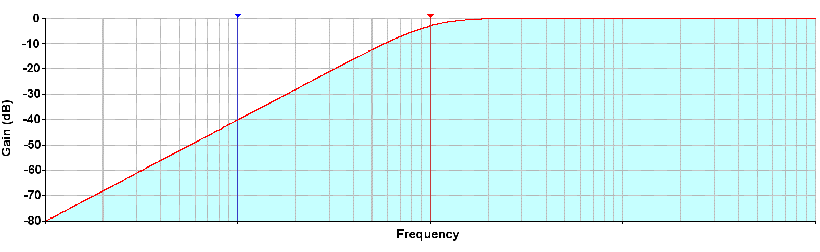
\includegraphics[width=\linewidth]{media/sloa093_HPF.pdf}
            \subcaption{}
            \label{fig:SimpleBodeExampleHPF}
        \end{minipage}
        \hspace{.04\linewidth}
        \begin{minipage}[H]{.45\linewidth}
            \centering
            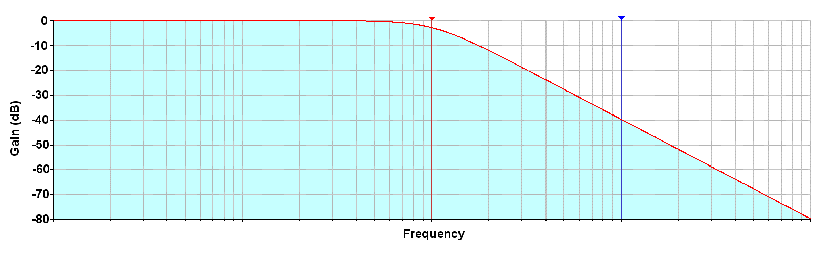
\includegraphics[width=\linewidth]{media/sloa093_LPF.pdf}
            \subcaption{}
            \label{fig:SimpleBodeExampleLPF}
        \end{minipage}
        \caption{Пример амплитудно-частотной характеристики простых передаточных функций: \ref{fig:SimpleBodeExampleHPF} High-Pass, или HPF, --- фильтр верхних частот, ослабляющий низкие частоты, \ref{fig:SimpleBodeExampleLPF} Low-Pass, или LPF, --- фильтр нижних частот, ослабляющий высокие частоты \emph{(буква «F» в сокращениях означает Filter --- фильтр) \parenciteit{}{FilterPassStopTypes:Image}}}
        \label{fig:SimpleBodeExample}
    \end{figure}
    \noindent Сложные функции, в свою очередь, таковы:
    \begin{figure}[H]
        \centering
        \begin{minipage}[H]{.45\linewidth}
            \centering
            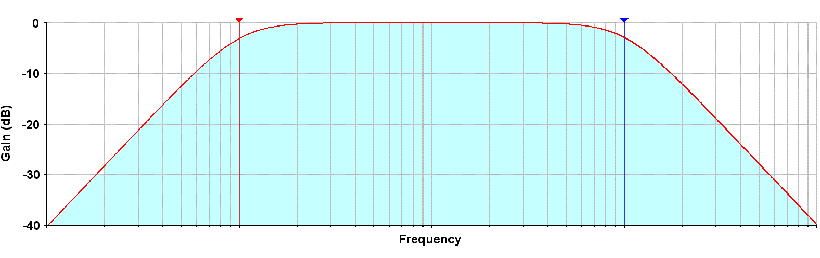
\includegraphics[width=\linewidth]{media/sloa093_BPF.pdf}
            \subcaption{}
            \label{fig:ComplicateBodeExampleBPF}
        \end{minipage}
        \hspace{.04\linewidth}
        \begin{minipage}[H]{.45\linewidth}
            \centering
            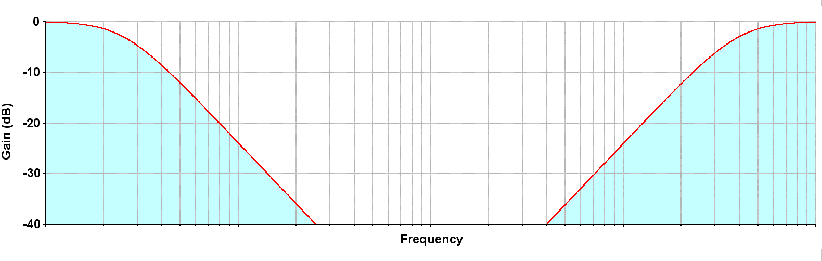
\includegraphics[width=\linewidth]{media/sloa093_BSF.pdf}
            \subcaption{}
            \label{fig:ComplicateBodeExampleBSF}
        \end{minipage}
        \\
        \begin{minipage}[H]{.45\linewidth}
            \centering
            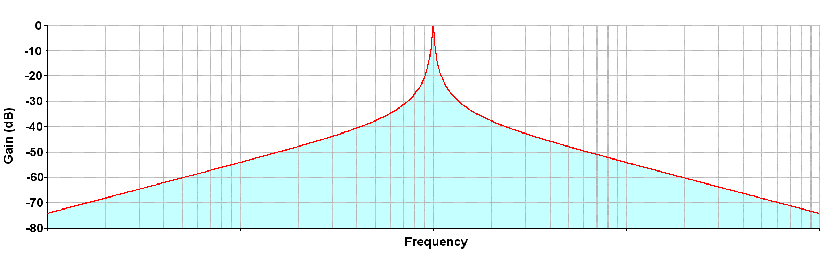
\includegraphics[width=\linewidth]{media/sloa093_NPF.pdf}
            \subcaption{}
            \label{fig:ComplicateBodeExampleNPF}
        \end{minipage}
        \hspace{.04\linewidth}
        \begin{minipage}[H]{.45\linewidth}
            \centering
            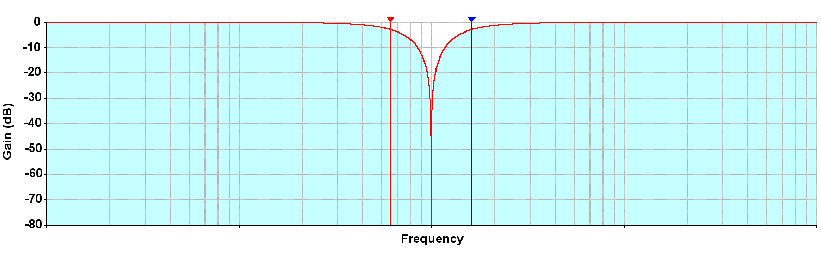
\includegraphics[width=\linewidth]{media/sloa093_NSF.pdf}
            \subcaption{}
            \label{fig:ComplicateBodeExampleNSF}
        \end{minipage}
        \caption{Пример амплитудно-частотной характеристики сложных передаточных функций: \ref{fig:ComplicateBodeExampleBPF} Band-Pass, или BPF, --- полосовой фильтр, пропускающий полосу частот, \ref{fig:ComplicateBodeExampleBSF} Band-Rejection, или BRF, --- режекторный фильтр, ослабляющий полосу частот, \ref{fig:ComplicateBodeExampleNPF} Narrow-Band-Pass, или NPF, --- узкополосный фильтр, пропускающий узкую полосу частот, \ref{fig:ComplicateBodeExampleNSF} Narrow-Band-Rejection, или NRF, --- узкополосный режекторный фильтр, ослабляющий узкую полосу частот \parenciteit{}{FilterPassStopTypes:Image}}
        \label{fig:ComplicateBodeExample}
    \end{figure}
    \clearpage

    \noindent Изменение порядка фильтра и параметра $\sigma$ проявляется в частотной области следующим образом, как на рисунке \ref{fig:FunctionShapesOrder}:
    \begin{figure}[H]
        \centering
        \begin{minipage}[H]{.45\linewidth}
            \centering
            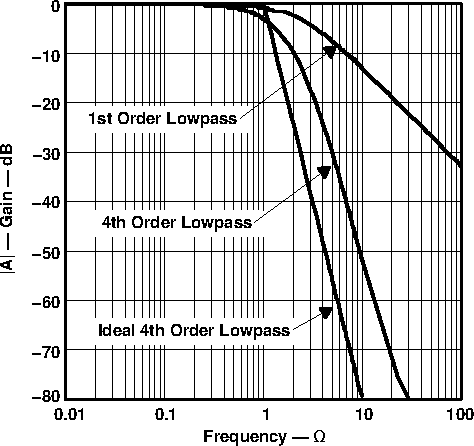
\includegraphics[width=\linewidth]{media/sloa088_order.pdf}
            \label{fig:FunctionOrder}
            \subcaption{Передаточные функции различной формы, получаемой изменением их порядка}
        \end{minipage}
        \hspace{.04\linewidth}
        \begin{minipage}[H]{.45\linewidth}
            \centering
            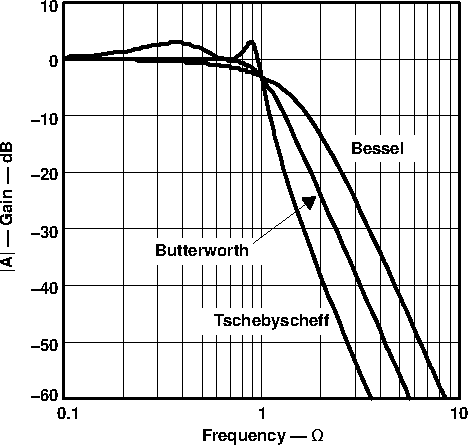
\includegraphics[width=\linewidth]{media/sloa088_shape.pdf}
            \label{fig:FunctionShapes}
            \subcaption{Передаточные функции различной формы, получаемой изменением $\sigma$}
        \end{minipage}
        \caption{Пример амплитудно-частотной характеристики нормированных передаточных функций фильтра нижних частот \emph{($\Omega$ обозначает нормированную частоту, то есть частота среза функции перенесена в значение $1$)} \parenciteit{}{SLOA088}}
        \label{fig:FunctionShapesOrder}
    \end{figure}
    % TRANSLATOR NOTE: original "puo al massimo contenerne una" has no clear referent; rendered as "может добавить не более одного порядка".
    \noindent Порядок аналогового фильтра можно изменить только добавлением компонентов в сеть\footnote{Это следует из знаний, изложенных в разделе \ref{sec:ElectronicsCalculusLaplace}} импедансов, поскольку пассивный электротехнический элемент может добавить не более одного порядка.
    Форма функции, в свою очередь, --- это компромисс между крутизной среза частот и тем, насколько плоской является та часть характеристики, которая должна остаться нетронутой.

    В моём проекте сдвиг фазы передаточной функции не имеет значения\footnote{Я считаю, что искусственный интеллект, который будет обрабатывать полученную информацию в будущих итерациях проекта, не зависит от сдвига фазы сигнала: достаточно, чтобы функция была одинаковой на всех сенсорных платах}, поэтому позволю себе пропустить описание характеристик различных форм функции.
    Вместо этого я представлю одну форму --- Баттерворта\footnote{Показана на рисунке \ref{fig:FunctionShapesOrder}}, наиболее эффективную с точки зрения того, насколько плоской остаётся нетронутая часть функции и насколько быстро она срезается на нужной частоте\footnote{Идея взята из объяснения в \parenciteit{p6}{SLOA088}}.
    Фильтр Баттерворта имеет крутизну спада\footnote{Называемую также rolloff rate} 20dB/dec\footnote{Эта единица показывает, на сколько уменьшается усиление фильтра при изменении частоты в десять раз} на порядок\footnote{Крутизну спада определённого порядка можно найти, умножив порядок фильтра на крутизну спада фильтра I порядка}.

    Чтобы лучше увидеть, как формируются передаточные функции при изменении параметра $\sigma$, я решил отложить его по одной из координатных осей и получил графики на рисунке \ref{fig:3DFUNCExample}:
    \begin{figure}[H]
        \centering
        \begin{minipage}[H]{.45\linewidth}
            \centering
            \newcommand{\plotDir}{datasets/s_plot_example_data}
            \newcommand{\plotName}{hpf_2}
            \import{\plotDir}{\plotName_def.tex}%
            \begin{tikzpicture}
                \begin{axis}[
                    width=\linewidth,
                    view = {20}{30},
                    % ymode=log,
                    xmin = \minX,
                    xmax = \maxX,
                    ymin = \minY,
                    ymax = \maxY,
                    zmin = \minZ,
                    zmax = \maxZ,
                    xtick = {\minTickX,\nextTickX,...,\maxTickX},
                    ytick = {\minTickY,\nextTickY,...,\maxTickY},
                    ztick = {\minTickZ,\nextTickZ,...,\maxTickZ},
                    xlabel={\legendX},
                    ylabel={\legendY},
                    zlabel={\legendZ},
                    label style={font=\footnotesize},
                    tick label style={font=\tiny},
                    smooth,
                    grid = both,
                    ymajorgrids = true,
                    line join=round,
                    clip=false
                ]
                \addplot3[
                    surf,
                    /pgfplots/colormap={bone}{rgb255=(0,0,0) rgb255=(84,84,116) rgb255=(167,199,199) rgb255=(240,240,240)},
                    opacity=0.9375,
                    shader=faceted interp,
                    patch type=coons,
                    z buffer=sort,
                    patch table=\plotDir/\plotName_anchors.csv
                ] table [col sep=comma,header=false] {\plotDir/\plotName.csv};
                \end{axis}
            \end{tikzpicture}
            \import{\plotDir}{All_plots_undef.tex}%
            \let\plotDir\undefined
            \let\plotName\undefined
            \subcaption{}
            \label{fig:HPF2Example}
        \end{minipage}
        \hspace{.04\linewidth}
        \begin{minipage}[H]{.45\linewidth}
            \centering
            \newcommand{\plotDir}{datasets/s_plot_example_data}
            \newcommand{\plotName}{lpf_2}
            \import{\plotDir}{\plotName_def.tex}%
            \begin{tikzpicture}
                \begin{axis}[
                    width=\linewidth,
                    view = {20}{30},
                    % ymode=log,
                    xmin = \minX,
                    xmax = \maxX,
                    ymin = \minY,
                    ymax = \maxY,
                    zmin = \minZ,
                    zmax = \maxZ,
                    xtick = {\minTickX,\nextTickX,...,\maxTickX},
                    ytick = {\minTickY,\nextTickY,...,\maxTickY},
                    ztick = {\minTickZ,\nextTickZ,...,\maxTickZ},
                    xlabel={\legendX},
                    ylabel={\legendY},
                    zlabel={\legendZ},
                    label style={font=\footnotesize},
                    tick label style={font=\tiny},
                    smooth,
                    grid = both,
                    ymajorgrids = true,
                    line join=round,
                    clip=false
                ]
                \addplot3[
                    surf,
                    /pgfplots/colormap={bone}{rgb255=(0,0,0) rgb255=(84,84,116) rgb255=(167,199,199) rgb255=(240,240,240)},
                    opacity=0.9375,
                    shader=faceted interp,
                    patch type=coons,
                    z buffer=sort,
                    patch table=\plotDir/\plotName_anchors.csv
                ] table [col sep=comma,header=false] {\plotDir/\plotName.csv};
                \end{axis}
            \end{tikzpicture}
            \import{\plotDir}{All_plots_undef.tex}%
            \let\plotDir\undefined
            \let\plotName\undefined
            \subcaption{}
            \label{fig:LPF2Example}
        \end{minipage}
        \\
        \begin{minipage}[H]{.45\linewidth}
            \centering
            \newcommand{\plotDir}{datasets/s_plot_example_data}
            \newcommand{\plotName}{bpf_2}
            \import{\plotDir}{\plotName_def.tex}%
            \begin{tikzpicture}
                \begin{axis}[
                    width=\linewidth,
                    view = {20}{30},
                    % ymode=log,
                    xmin = \minX,
                    xmax = \maxX,
                    ymin = \minY,
                    ymax = \maxY,
                    zmin = \minZ,
                    zmax = \maxZ,
                    xtick = {\minTickX,\nextTickX,...,\maxTickX},
                    ytick = {\minTickY,\nextTickY,...,\maxTickY},
                    ztick = {\minTickZ,\nextTickZ,...,\maxTickZ},
                    xlabel={\legendX},
                    ylabel={\legendY},
                    zlabel={\legendZ},
                    label style={font=\footnotesize},
                    tick label style={font=\tiny},
                    smooth,
                    grid = both,
                    ymajorgrids = true,
                    line join=round,
                    clip=false
                ]
                \addplot3[
                    surf,
                    /pgfplots/colormap={bone}{rgb255=(0,0,0) rgb255=(84,84,116) rgb255=(167,199,199) rgb255=(240,240,240)},
                    opacity=0.9375,
                    shader=faceted interp,
                    patch type=coons,
                    z buffer=sort,
                    patch table=\plotDir/\plotName_anchors.csv
                ] table [col sep=comma,header=false] {\plotDir/\plotName.csv};
                \end{axis}
            \end{tikzpicture}
            \import{\plotDir}{All_plots_undef.tex}%
            \let\plotDir\undefined
            \let\plotName\undefined
            \subcaption{}
            \label{fig:BPF2Example}
        \end{minipage}
        \hspace{.04\linewidth}
        \begin{minipage}[H]{.45\linewidth}
            \centering
            \newcommand{\plotDir}{datasets/s_plot_example_data}
            \newcommand{\plotName}{bpf_4}
            \import{\plotDir}{\plotName_def.tex}%
            \begin{tikzpicture}
                \begin{axis}[
                    width=\linewidth,
                    view = {20}{30},
                    % ymode=log,
                    xmin = \minX,
                    xmax = \maxX,
                    ymin = \minY,
                    ymax = \maxY,
                    zmin = \minZ,
                    zmax = \maxZ,
                    xtick = {\minTickX,\nextTickX,...,\maxTickX},
                    ytick = {\minTickY,\nextTickY,...,\maxTickY},
                    ztick = {\minTickZ,\nextTickZ,...,\maxTickZ},
                    xlabel={\legendX},
                    ylabel={\legendY},
                    zlabel={\legendZ},
                    label style={font=\footnotesize},
                    tick label style={font=\tiny},
                    smooth,
                    grid = both,
                    ymajorgrids = true,
                    line join=round,
                    clip=false
                ]
                \addplot3[
                    surf,
                    /pgfplots/colormap={bone}{rgb255=(0,0,0) rgb255=(84,84,116) rgb255=(167,199,199) rgb255=(240,240,240)},
                    opacity=0.9375,
                    shader=faceted interp,
                    patch type=coons,
                    z buffer=sort,
                    patch table=\plotDir/\plotName_anchors.csv
                ] table [col sep=comma,header=false] {\plotDir/\plotName.csv};
                \end{axis}
            \end{tikzpicture}
            \import{\plotDir}{All_plots_undef.tex}%
            \let\plotDir\undefined
            \let\plotName\undefined
            \subcaption{}
            \label{fig:BPF4Example}
        \end{minipage}
        \begin{minipage}[H]{.45\linewidth}
            \centering
            \newcommand{\plotDir}{datasets/s_plot_log_example_data}
            \newcommand{\plotName}{hpf_2}
            \import{\plotDir}{\plotName_def.tex}%
            \begin{tikzpicture}
                \begin{axis}[
                    width=\linewidth,
                    view = {70}{30},
                    ymode=log,
                    log ticks with fixed point,
                    xmin = \minX,
                    xmax = \maxX,
                    ymin = \minY,
                    ymax = \maxY,
                    zmin = \minZ,
                    zmax = \maxZ,
                    xtick = {\minTickX,\nextTickX,...,\maxTickX},
                    ytick = {\minTickY,\nextTickY,...,\maxTickY},
                    ztick = {\minTickZ,\nextTickZ,...,\maxTickZ},
                    xlabel={\legendX},
                    ylabel={\legendY},
                    zlabel={\legendZ},
                    label style={font=\footnotesize},
                    tick label style={font=\tiny},
                    smooth,
                    grid = both,
                    ymajorgrids = true,
                    line join=round,
                    clip=false,
                    y tick label style = {rotate=-60, anchor=west}
                ]
                \addplot3[
                    surf,
                    /pgfplots/colormap={bone}{rgb255=(0,0,0) rgb255=(84,84,116) rgb255=(167,199,199) rgb255=(240,240,240)},
                    opacity=0.9375,
                    shader=faceted interp,
                    patch type=coons,
                    z buffer=sort,
                    patch table=\plotDir/\plotName_anchors.csv
                ] table [col sep=comma,header=false] {\plotDir/\plotName.csv};
                \end{axis}
            \end{tikzpicture}
            \import{\plotDir}{All_plots_undef.tex}%
            \let\plotDir\undefined
            \let\plotName\undefined
            \subcaption{}
            \label{fig:HPF2logExample}
        \end{minipage}
        \hspace{.04\linewidth}
        \begin{minipage}[H]{.45\linewidth}
            \centering
            \newcommand{\plotDir}{datasets/s_plot_log_example_data}
            \newcommand{\plotName}{lpf_2}
            \import{\plotDir}{\plotName_def.tex}%
            \begin{tikzpicture}
                \begin{axis}[
                    width=\linewidth,
                    view = {70}{30},
                    ymode=log,
                    log ticks with fixed point,
                    xmin = \minX,
                    xmax = \maxX,
                    ymin = \minY,
                    ymax = \maxY,
                    zmin = \minZ,
                    zmax = \maxZ,
                    xtick = {\minTickX,\nextTickX,...,\maxTickX},
                    ytick = {\minTickY,\nextTickY,...,\maxTickY},
                    ztick = {\minTickZ,\nextTickZ,...,\maxTickZ},
                    xlabel={\legendX},
                    ylabel={\legendY},
                    zlabel={\legendZ},
                    label style={font=\footnotesize},
                    tick label style={font=\tiny},
                    smooth,
                    grid = both,
                    ymajorgrids = true,
                    line join=round,
                    clip=false,
                    y tick label style = {rotate=-60, anchor=west}
                ]
                \addplot3[
                    surf,
                    /pgfplots/colormap={bone}{rgb255=(0,0,0) rgb255=(84,84,116) rgb255=(167,199,199) rgb255=(240,240,240)},
                    opacity=0.9375,
                    shader=faceted interp,
                    patch type=coons,
                    z buffer=sort,
                    patch table=\plotDir/\plotName_anchors.csv
                ] table [col sep=comma,header=false] {\plotDir/\plotName.csv};
                \end{axis}
            \end{tikzpicture}
            \import{\plotDir}{All_plots_undef.tex}%
            \let\plotDir\undefined
            \let\plotName\undefined
            \subcaption{}
            \label{fig:LPF2logExample}
        \end{minipage}
        \\
        \begin{minipage}[H]{.45\linewidth}
            \centering
            \newcommand{\plotDir}{datasets/s_plot_log_example_data}
            \newcommand{\plotName}{bpf_2}
            \import{\plotDir}{\plotName_def.tex}%
            \begin{tikzpicture}
                \begin{axis}[
                    width=\linewidth,
                    view = {70}{30},
                    ymode=log,
                    log ticks with fixed point,
                    xmin = \minX,
                    xmax = \maxX,
                    ymin = \minY,
                    ymax = \maxY,
                    zmin = \minZ,
                    zmax = \maxZ,
                    xtick = {\minTickX,\nextTickX,...,\maxTickX},
                    ytick = {\minTickY,\nextTickY,...,\maxTickY},
                    ztick = {\minTickZ,\nextTickZ,...,\maxTickZ},
                    xlabel={\legendX},
                    ylabel={\legendY},
                    zlabel={\legendZ},
                    label style={font=\footnotesize},
                    tick label style={font=\tiny},
                    smooth,
                    grid = both,
                    ymajorgrids = true,
                    line join=round,
                    clip=false,
                    y tick label style = {rotate=-60, anchor=west}
                ]
                \addplot3[
                    surf,
                    /pgfplots/colormap={bone}{rgb255=(0,0,0) rgb255=(84,84,116) rgb255=(167,199,199) rgb255=(240,240,240)},
                    opacity=0.9375,
                    shader=faceted interp,
                    patch type=coons,
                    z buffer=sort,
                    patch table=\plotDir/\plotName_anchors.csv
                ] table [col sep=comma,header=false] {\plotDir/\plotName.csv};
                \end{axis}
            \end{tikzpicture}
            \import{\plotDir}{All_plots_undef.tex}%
            \let\plotDir\undefined
            \let\plotName\undefined
            \subcaption{}
            \label{fig:BPF2logExample}
        \end{minipage}
        \hspace{.04\linewidth}
        \begin{minipage}[H]{.45\linewidth}
            \centering
            \newcommand{\plotDir}{datasets/s_plot_log_example_data}
            \newcommand{\plotName}{bpf_4}
            \import{\plotDir}{\plotName_def.tex}%
            \begin{tikzpicture}
                \begin{axis}[
                    width=\linewidth,
                    view = {70}{30},
                    ymode=log,
                    log ticks with fixed point,
                    xmin = \minX,
                    xmax = \maxX,
                    ymin = \minY,
                    ymax = \maxY,
                    zmin = \minZ,
                    zmax = \maxZ,
                    xtick = {\minTickX,\nextTickX,...,\maxTickX},
                    ytick = {\minTickY,\nextTickY,...,\maxTickY},
                    ztick = {\minTickZ,\nextTickZ,...,\maxTickZ},
                    xlabel={\legendX},
                    ylabel={\legendY},
                    zlabel={\legendZ},
                    label style={font=\footnotesize},
                    tick label style={font=\tiny},
                    smooth,
                    grid = both,
                    ymajorgrids = true,
                    line join=round,
                    clip=false,
                    y tick label style = {rotate=-60, anchor=west}
                ]
                \addplot3[
                    surf,
                    /pgfplots/colormap={bone}{rgb255=(0,0,0) rgb255=(84,84,116) rgb255=(167,199,199) rgb255=(240,240,240)},
                    opacity=0.9375,
                    shader=faceted interp,
                    patch type=coons,
                    z buffer=sort,
                    patch table=\plotDir/\plotName_anchors.csv
                ] table [col sep=comma,header=false] {\plotDir/\plotName.csv};
                \end{axis}
            \end{tikzpicture}
            \import{\plotDir}{All_plots_undef.tex}%
            \let\plotDir\undefined
            \let\plotName\undefined
            \subcaption{}
            \label{fig:BPF4logExample}
        \end{minipage}
        \caption{Четыре передаточные функции разных типов и порядков с осью усиления в логарифмическом масштабе и осью частот $\omega$ в линейном масштабе на \ref{fig:HPF2Example} \ref{fig:LPF2Example} \ref{fig:BPF2Example} \ref{fig:BPF4Example} и в логарифмическом масштабе на \ref{fig:HPF2logExample} \ref{fig:LPF2logExample} \ref{fig:BPF2logExample} \ref{fig:BPF4logExample}}
        \label{fig:3DFUNCExample}
    \end{figure}
    \clearpage

    \subsubsection{Электротехника \& фильтры}
    Фильтры, которые мы рассмотрели в разделе \ref{sec:ElectronicsCalculusLaplace} на рисунках \ref{fig:CapFilterExample} и \ref{fig:CapFilterExample2}, увеличивают выходное сопротивление, и единственное, что они делают, --- ослабляют сигнал\footnote{В реальном мире для считывания напряжения с проводника через него должен протекать ток, и из-за импеданса фильтра (даже для частот, которые не должны ослабляться) напряжение падает}.
    Следовательно, чтобы повысить порядок фильтра, нужно усиливать сигнал.
    Первая идея --- поставить последовательно с фильтром операционный усилитель (ОУ), но это не лучший выбор, потому что существуют активные фильтры, то есть фильтры, в топологию которых уже входит усилитель.
    Самые простые и популярные из них --- SK, или Sallen-Key (Саллена--Ки), и MFB, или Multiple-Feedback-Filter (с многопетлевой обратной связью), показанные на следующем рисунке \ref{fig:SKMFBSchematic}
    \begin{figure}[H]
        \centering
        \begin{minipage}[H]{.45\linewidth}
            \centering
            \begin{tikzpicture}[transform shape, use fpu reciprocal, scale=.75]
                \draw (0,0)
                    to[R, l=$R_1$, -*] ++(2,0)
                    coordinate(C1)
    
                    to[R, l=$R_2$, -*] ++(2,0)
                    coordinate(C2)
    
                    (C2)
                    -- ++(1.25,0)
                    node[op amp, noinv input up, fill=cyan!20, anchor=+](OA1){\texttt{OA1}}
    
                    (C2)
                    to[C, l=$C_2$] ++(0,-2)
                    node[tlground]{}
    
                    (OA1.-)
                    -- ++ (-.25,0)
                    -- ++(0,-1.75)
                    coordinate(Rg1Rg2)
                    to[R, l=$R_{G1}$, *-] (Rg1Rg2-|OA1.out)
                    to[short, -*] (OA1.out)
    
                    (Rg1Rg2) to[R, l=$R_{G2}$] ++(0,-2)
                    node[tlground]{}
    
                    (C1)
                    -- ++(0,1.5)
                    coordinate(R1start)
                    to[C, l=$C_1$] (R1start-|OA1.out)
                    -- (OA1.out)
    
                    (OA1.up)
                    node[vcc]{$V_{CC}$}
    
                    (OA1.down)
                    node[ground]{}
    
                    (OA1.out) ++(.5,0)
                    node[right]{$U_{out}$}
                    to[short, o-] ++(-.5,0)
    
                    (0,0)
                    node[left]{$U_{in}$}
                    to[short, o-] ++(0,0)
                    ;
            \end{tikzpicture}
            \subcaption{Топология Sallen-Key; её преимущество в том, что значения $\sigma$ и усиления независимы \emph{($R_{GX}$ задают усиление, $RX$ и $CX$ --- $\sigma$)}}
            \label{fig:SKSchematic}
        \end{minipage}
        \hspace{.04\linewidth}
        \begin{minipage}[H]{.45\linewidth}
            \centering
            \begin{tikzpicture}[transform shape, use fpu reciprocal, scale=.75]
                \draw (0,0)
                    to[R, l=$R_1$, -*] ++(2,0)
                    coordinate(C1)
    
                    to[R, l=$R_3$, -*] ++(2,0)
                    coordinate(C2)
                    -- ++(.75,0)
                    node[op amp, noinv input down, fill=cyan!20, anchor=-](OA1){\texttt{OA1}}
    
                    (OA1.+)
                    -- ++(-.25,0)
                    node[ground]{}
    
                    (OA1.up)
                    node[vcc]{$V_{CC}$}
    
                    (OA1.down)
                    node[ground]{}
    
                    (C1)
                    to[C, l=$C_1$] ++(0,-2)
                    node[tlground]{}
    
                    (C2)
                    -- ++(0,1.5)
                    coordinate(R2start)
                    to[C, l=$C_2$, -*] (R2start-|OA1.out)
                    coordinate(R2)
                    to[short, -*] (OA1.out)
    
                    (C1)
                    -- ++(0,2.5)
                    coordinate(C3start)
                    to[R, l=$R_2$] (C3start-|OA1.out)
                    -- (R2)
    
                    (OA1.out) ++(.5,0)
                    node[right]{$U_{out}$}
                    to[short, o-] ++(-.5,0)
    
                    (0,0)
                    node[left]{$U_{in}$}
                    to[short, o-] ++(0,0)
                    ;
            \end{tikzpicture}
            \subcaption{Топология Multiple-Feedback; её преимущества --- меньше пассивных компонентов и меньшая чувствительность к изменению их номиналов \emph{(номиналы пассивных компонентов не вполне постоянны и в основном зависят от температуры окружающей среды)}; кроме того, она инвертирует сигнал}
            \label{fig:MFBSchematic}
        \end{minipage}
        \hspace{.04\linewidth}
        \caption{Схемы двух активных ФНЧ II порядка}
        \label{fig:SKMFBSchematic}
    \end{figure}


    \noindent Чтобы вычислить передаточную функцию этих фильтров, я применил следующий метод:
    \begin{enumerate}[label=\emph{(\roman*)}]
        \item Использовать функции, полученные из преобразования Лапласа для пассивных компонентов.
        \item С помощью законов Ома и законов Кирхгофа составить уравнения схемы, то есть соотношения между различными токами в схеме
        \item Составить систему уравнений, описывающую соотношения между различными токами, заданными в виде $I=\frac{U}{Z(s)}$
        \item Исключить все токи, кроме $\frac{U_{out}}{U_{in}}$
        \item Выразить $\frac{U_{out}}{U_{in}}$ в одной части уравнения
    \end{enumerate}
    Так мне удалось описать различные варианты двух топологий схемы; заинтересованный читатель может найти их на страницах раздела расчётов \ref{sec:Calculations}.

    \clearpage
    \section{Сенсорная плата}\label{sec:Sensorboard}
    \subsection{Характеристики}\label{sec:SensorboardCharacteristics}
    \begin{enumerate}[label=\emph{(\arabic*)}]
        \item Устойчивость к внешним шумам, то есть способность выделять нужную часть сигнала
        \item Устойчивость к ударам
        \item Вносить как можно меньше внутреннего или внешнего шума в схему, чтобы сохранить высокое качество сигнала: стремиться к разрешению $12bit$\footcite[p9]{EMGBitdepth}
        \item Модульность
        \item Малые размеры
    \end{enumerate}

    \subsection{Проектирование}\label{sec:SensorboardDesign}
    Чтобы принимать адекватные решения, сначала нужно изучить конкретную ситуацию.
    \subsubsection{Изучение входа}\label{sec:SensorboardDesignInput}
    Чтобы изучить вход, нужно знать и об источнике.
    Сигналы, исходящие из спинного мозга и называемые APs\footnote{Action potentials, то есть потенциалы действия \parenciteit{}{MerlettiMuceli}}, распространяются по нервам по закону «всё или ничего»\footnote{Обусловлено свойствами нервных клеток, а именно потенциал-зависимыми натриевыми каналами \parenciteit{}{SodiumChannel:Wiki}, которые создают цепную реакцию.} --- цепной реакции, которая делает\footnote{Нейроны в неактивном состоянии имеют отрицательный потенциал около $-70mV$ \parenciteit{}{AP:Wiki}} нейроны положительными\footnote{Если потенциал нейрона превышает $-55mV$, потенциал-зависимые натриевые каналы открываются, впуская катионы натрия, и нейрон приобретает положительный заряд \parenciteit{}{AP:Wiki}} один за другим, пока сигнал не дойдёт до иннервации мышцы \footnote{Соединение нерва с мышцей \parenciteit{«NMJ» и «innervation zone» p3}{MerlettiMuceli}}.
    Сразу после этого начинается вторая цепная реакция --- в мышце.
    Мышечные клетки сокращаются одна за другой, тем самым активируя остальные, и сигнал мышцы \todo{Добавить пример разложения сигнала по частотам и чистый сигнал} многократно усиливается, создавая сигнал, как на рисунке \ref{fig:ExampleEMGSignal} \ref{fig:ExampleEMGSignalTime}

    % TRANSLATOR NOTE: the first footnote below is unfinished in the original; translated as-is.
    Стоит отметить, что интенсивность суммарного сигнала\footnote{Нужно понимать, что в данном случае разделения нет } имеет наибольшую амплитуду в области низких частот\footnote{Отчасти это может быть и составляющая фликкер-шума (розового шума) схем датчика}.

    Когда сигнал по нерву приходит к иннервации мышцы, мышечные клетки начинают сокращаться\footnote{Сокращаясь, они в свою очередь генерируют дополнительный сигнал, тем самым усиливая его и для других мышечных клеток}, также создавая цепную реакцию за счёт определённых электрохимических процессов.
    На поверхности кожи человека в момент сокращения расположенных под ней мышц присутствуют электрические поля.
    Пиковое напряжение между электродом, принимающим сигнал, и электродом, подключённым к электрически нейтральному\footnote{Где электрические поля отсутствуют} участку кожи, составляет $10mV$ \footcite[p435]{Naik}\: \footcite[p1]{Xiaoou}.
    Частота полезного сигнала типичной мышцы лежит в основном в диапазоне $20-500Hz$\footcite[p1]{EMGFreq}.
    Распространение сигнала не мгновенно, его скорость составляет $3-5m/s$\footcite[p2]{MerlettiMuceli}.
    Сопротивление кожи человека, которое всегда нужно учитывать из-за его влияния на пиковый ток, может составлять от $1k\Omega$ до $100k\Omega$\footcite[``Under dry conditions, the resistance offered by the human body may be as high as 100,000Ohms.  Wet or broken skin may drop the body's resistance to 1,000 Ohms'', p7]{ElectricalDeaths}.
    Разброс приведённых выше данных зависит от качества контакта с кожей и правильности размещения электродов.

    \begin{figure}[H]
        \centering
        \begin{minipage}[H]{\linewidth}
            \raggedright
            \begin{tikzpicture}
                \begin{axis}[
                    axis x line=bottom,
                    axis y line*=left,
                    ylabel style={rotate=-90},
                    xlabel={$t[ms]$},
                    ylabel={$U[V]\cdot k$},
                    legend entries={$($Канал $1)$, $($Канал $2)$, $($Канал $3)$, $($Канал $4)$, $($Канал $5)$, $($Канал $6)$, $($Канал $7)$, $($Канал $8)$},
                    legend pos=north east,
                    height=.4\textwidth,
                    width=.85\textwidth,
                    smooth,
                    clip=true,
                    xmin=2500,
                    xmax=17500,
                    axis_style_default_data,
                    colormap/twilight,
                    ymajorgrids=true,
                    xmajorgrids=false,
                    grid style=dashed,
                    cycle list={[colors of colormap={130,200,280,370,630,720,800,870},]},
                    every axis plot/.append style={mark=none, thick, draw opacity=.7},
                    ]
                    \begin{scope}[blend group=hard light]
                        \addplot table [x=time, y=channel1, col sep=comma]{datasets/cf_fft_hand_muscles/snip_s.csv};
                        \addplot table [x=time, y=channel2, col sep=comma]{datasets/cf_fft_hand_muscles/snip_s.csv};
                        \addplot table [x=time, y=channel3, col sep=comma]{datasets/cf_fft_hand_muscles/snip_s.csv};
                        \addplot table [x=time, y=channel4, col sep=comma]{datasets/cf_fft_hand_muscles/snip_s.csv};
                        \addplot table [x=time, y=channel5, col sep=comma]{datasets/cf_fft_hand_muscles/snip_s.csv};
                        \addplot table [x=time, y=channel6, col sep=comma]{datasets/cf_fft_hand_muscles/snip_s.csv};
                        \addplot table [x=time, y=channel7, col sep=comma]{datasets/cf_fft_hand_muscles/snip_s.csv};
                        \addplot table [x=time, y=channel8, col sep=comma]{datasets/cf_fft_hand_muscles/snip_s.csv};
                    \end{scope}
                \end{axis}
            \end{tikzpicture}
            \subcaption{Фрагмент сигнала из 8 каналов, с $($Канал $1)$ по $($Канал $8)$, в зависимости от времени \emph{(рост амплитуды соответствует напряжению мышц)}}
            \label{fig:ExampleEMGSignalTime}
        \end{minipage}
        \vspace{3ex}
        \begin{minipage}[H]{\linewidth}
            \raggedright
            \begin{tikzpicture}
                \begin{axis}[
                    axis x line=bottom,
                    axis y line*=left,
                    ylabel style={rotate=-90},
                    xlabel={$f[Hz]$},
                    ylabel={$U[V]\cdot k$},
                    legend entries={$(a)$ Всего, $(b)$ Шум},
                    legend pos=north east,
                    height=.305\textwidth,
                    width=.8\textwidth,
                    smooth,
                    clip=true,
                    xmode=log,
                    ymode=log,
                    domain=1:500,
                    samples=50,
                    xmin=1,
                    xmax=500,
                    ymin=2e-8,
                    ymax=3e-5,
                    axis_style_default_data,
                    colormap/twilight_shifted,
                    ymajorgrids=true,
                    xmajorgrids=true,
                    grid style=dashed,
                    cycle list={[colors of colormap={145,250},]},
                    every axis plot/.append style={mark=none, thick, draw opacity=.7},
                    ]
                    \begin{scope}[blend group=hard light]
                        \addplot table [x=freqs, y=spect, col sep=comma]{datasets/cf_fft_hand_muscles/sfft.csv};
                        \addplot table [x=freqs, y=spect, col sep=comma]{datasets/cf_fft_hand_muscles/noise_sfft.csv};
                    \end{scope}
                \end{axis}
            \end{tikzpicture}
            \subcaption{Частотный спектр общего среднего $(a)$ и среднего шума $(b)$}
            \label{fig:ExampleEMGSignalFFT}
        \end{minipage}
        \vspace{3ex}
        \begin{minipage}[H]{\linewidth}
            \raggedright
            \begin{tikzpicture}
                \begin{axis}[
                    axis x line=bottom,
                    axis y line*=left,
                    ylabel style={rotate=-90},
                    xlabel={$f[Hz]$},
                    ylabel={$U[V]\cdot k$},
                    legend entries={$(c)$ Раскрытая ладонь (без очистки), $(d)$ Кулак (без очистки)},
                    legend pos=north east,
                    height=.305\textwidth,
                    width=.8\textwidth,
                    smooth,
                    clip=true,
                    xmode=log,
                    ymode=log,
                    domain=1:500,
                    samples=50,
                    xmin=1,
                    xmax=500,
                    ymin=2e-8,
                    ymax=3e-5,
                    axis_style_default_data,
                    colormap/twilight_shifted,
                    ymajorgrids=true,
                    xmajorgrids=true,
                    grid style=dashed,
                    cycle list={[colors of colormap={280,720},]},
                    every axis plot/.append style={mark=none, thick, draw opacity=.7},
                    ]
                    \begin{scope}[blend group=hard light]
                        \addplot table [x=freqs, y=spect, col sep=comma]{datasets/cf_fft_hand_muscles/extended_sfft.csv};
                        \addplot table [x=freqs, y=spect, col sep=comma]{datasets/cf_fft_hand_muscles/fist_sfft.csv};
                    \end{scope}
                \end{axis}
            \end{tikzpicture}
            \subcaption{Частотный спектр среднего, без вычитания шумов, при жесте «раскрытая ладонь» $(c)$ и при жесте «кулак» $(d)$}
            \label{fig:ExampleEMGSignalFFTGestures}
        \end{minipage}
        \vspace{3ex}
        \begin{minipage}[H]{\linewidth}
            \raggedright
            \begin{tikzpicture}
                \begin{axis}[
                    axis x line=bottom,
                    axis y line*=left,
                    ylabel style={rotate=-90},
                    xlabel={$f[Hz]$},
                    ylabel={$U[V]\cdot k$},
                    legend entries={$(e)$ Раскрытая ладонь, $(f)$ Кулак},
                    legend pos=north east,
                    height=.305\textwidth,
                    width=.8\textwidth,
                    smooth,
                    clip=true,
                    xmode=log,
                    ymode=log,
                    domain=1:500,
                    samples=50,
                    xmin=1,
                    xmax=500,
                    ymin=2e-8,
                    ymax=3e-5,
                    axis_style_default_data,
                    colormap/twilight_shifted,
                    ymajorgrids=true,
                    xmajorgrids=true,
                    grid style=dashed,
                    cycle list={[colors of colormap={750,855},]},
                    every axis plot/.append style={mark=none, thick, draw opacity=.7},
                    ]
                    \begin{scope}[blend group=hard light]
                        \addplot table [x=freqs, y=spect, col sep=comma]{datasets/cf_fft_hand_muscles/extended_filt_sfft.csv};
                        \addplot table [x=freqs, y=spect, col sep=comma]{datasets/cf_fft_hand_muscles/fist_filt_sfft.csv};
                    \end{scope}
                \end{axis}
            \end{tikzpicture}
            \subcaption{Частотный спектр среднего, после вычитания шумов, при жесте «раскрытая ладонь» $(e)$ и при жесте «кулак» $(f)$}
            \label{fig:ExampleEMGSignalFFTGesturesPure}
        \end{minipage}
        \caption{Пример сигнала AP мышцы, измеренного в $U[V]\cdot k$ \emph{(}$k$\emph{ обозначает неизвестное усиление считанных и оцифрованных напряжений, представленных на графиках)}, в зависимости от времени на \ref{fig:ExampleEMGSignalTime} и разложенного по частотам \emph{(то есть в частотном спектре)} с помощью преобразования Фурье на графиках \ref{fig:ExampleEMGSignalFFT}, \ref{fig:ExampleEMGSignalFFTGestures}, \ref{fig:ExampleEMGSignalFFTGesturesPure} \emph{\parenciteit{}{EMGData}}}
        \label{fig:ExampleEMGSignal}
    \end{figure}

    \subsubsection{Изучение выхода}\label{sec:SensorboardDesignOutput}
    Выход полностью зависит от выбранного АЦП.
    Достаточно, чтобы выходной сигнал аналоговой схемы\footnote{Выход фильтров} укладывался в заданные пределы микросхемы.
    Как хорошую практику я считаю, что максимальную амплитуду сигнала нужно умножить на 4, чтобы получить пределы входа АЦП и предотвратить клиппинг сигнала.
    Выход, разумеется, не может быть отрицательным, чтобы не рисковать выйти за пределы спецификаций АЦП.
    Решением был бы прецизионный однополупериодный\footnote{Сигнал будет срезаться, если опустится ниже определённого порога напряжения} или двухполупериодный\footnote{Сигнал инвертируется, если опустится ниже определённого порога напряжения} выпрямитель.
    Максимальное напряжение тоже не должно выходить за пределы, поэтому я использовал бы прецизионные линейные источники напряжения\footnote{Напряжение должно быть стабильным, а преобразователь не должен создавать проблем с EMI, поэтому импульсные (switch-mode) DC-DC-преобразователи нельзя использовать напрямую, как сказано в разделе \ref{sec:MotherboardDesignSupply}}, не превышающие максимально допустимого напряжения.

    \subsubsection{Схема} \label{sec:SensorBoardSchematic}
    Схема сенсорной платы прежде всего должна устранять внешние помехи, приходящие на электроды.
    Можно воспользоваться задержкой распространения сигнала по мышце: внешние помехи, приходящие на два\footnote{Минимальное число электродов, необходимое для ослабления большей части помех в сигнале} электрода, как правило, мгновенны, как радиосигналы, тогда как разница в расстоянии между электродами влияет на считываемый ими сигнал мышцы.
    Поэтому нам достаточно вычесть один сигнал из другого.
    В практике проектирования схем существует активный компонент, предназначенный для вычитания\footnote{При этом он остаётся аналоговым} двух сигналов, --- INA, или инструментальный усилитель (Instrumentation Amplifier).
    \begin{figure}[H]
        \centering
        \hspace{.02\linewidth}
        \begin{minipage}[H]{.24\linewidth}
            \centering
            \begin{tikzpicture}[transform shape, use fpu reciprocal, scale=.75]
                \draw (0,0)
                    node[inst amp, noinv input up, fill=cyan!20](INA1){\texttt{INA1}}
                    \opampPMCenter{INA1}

                    (INA1.+) ++(-.5,0)
                    node[left]{$U_1$}
                    to[short, o-] ++(.5,0)

                    (INA1.-) ++(-.5,0)
                    node[left]{$U_2$}
                    to[short, o-] ++(.5,0)

                    (INA1.up)
                    node[vcc]{$V_{CC}$}

                    (INA1.down)
                    node[vee]{$V_{EE}$}

                    (INA1.out) ++(.5,0)
                    node[right]{$U_{out}$}
                    to[short, o-] ++(-.5,0)
                    ;
            \end{tikzpicture}
            \subcaption{Условное обозначение INA, который питается от двух источников напряжения: положительного $V_{CC}$ и отрицательного $V_{EE}$; $U_1$ --- входной сигнал на входе $+$, $U_2$ --- другой входной сигнал на инвертирующем входе $-$ \emph{(умножает сигнал на $-1$)}, $U_{out}$ --- выход}
            \label{fig:INASymbol}
        \end{minipage}
        \hspace{.04\linewidth}
        \begin{minipage}[H]{.64\linewidth}
            \centering
            \begin{tikzpicture}[transform shape, use fpu reciprocal, scale=.75]
                \draw (0,0)
                    node[op amp, noinv input up, fill=cyan!20](OA1){\texttt{OA1}}
                    \opampPMCenter{OA1};
                \draw (OA1.+) ++(-1,0)
                    node[left]{$U_1$}
                    to[short, o-] ++(1,0);
                \draw (OA1.out)
                    to[short, -*] ++(0,0)
                    to[R, l=$R_1$, -*] ++(0,-2)
                    coordinate(OA1-R1Rg)
                    to[R, l=$R_{G}$, -*] ++(0,-2)
                    coordinate(OA2-R1Rg)
                    to[R, l=$R_1$, -*] ++(0,-2)
                    node[op amp, fill=cyan!20, anchor=out](OA2){\texttt{OA2}};
                \draw (OA2.+) ++(-1,0)
                    node[left]{$U_2$}
                    to[short, o-] ++(1,0);
                \draw (OA1-R1Rg)
                    -- (OA1.- |- OA1-R1Rg)
                    -- (OA1.-);
                \draw (OA2-R1Rg)
                    -- (OA2.- |- OA2-R1Rg)
                    -- (OA2.-);
                \draw (OA1.out)
                    to[R, l=$R_2$, -*] ++(2,0)
                    coordinate(R2R3-up);
                \draw (OA2.out)
                    to[R, l=$R_2$, -*] ++(2,0)
                    coordinate(R2R3-down);
                \draw ($(R2R3-up)!.5!(R2R3-down)$) ++(opampPMCenter)
                    node[op amp, noinv input up, fill=cyan!20, anchor=center](OA3){\texttt{OA3}};
                \draw (OA3.+)
                    -- (R2R3-up);
                \draw (OA3.-)
                    -- (R2R3-down);
                \draw (R2R3-up)
                    to[R, l=$R_3$] ++(2,0)
                    -- (OA3.out |- R2R3-up)
                    to[short, -*](OA3.out)
                    coordinate(OA3-Vout);
                \draw (OA3.out) ++(1,0)
                    node[right]{$U_{out}$}
                    to[short, o-] ++(-1,0);
                \draw (R2R3-down)
                    to[R, l=$R_3$] ++(2,0)
                    -- (OA3.out |- R2R3-down)
                    node[ground]{};
            \end{tikzpicture}
            \subcaption{Внутреннее устройство INA: усиление задаётся резистором $R_G$, который обычно не входит в микросхему, чтобы разработчик схемы мог сам выбрать коэффициент}
            \label{fig:INAInternalSchematic}
        \end{minipage}
        \hspace{.04\linewidth}
        \caption{Схемы типового INA}
        \label{fig:INASchematic}
    \end{figure}

    Второй тип помех относится к частотному спектру, который мы определили по данным научных статей и по набору данных на графике на рисунке \ref{fig:ExampleEMGSignal}.
    Именно здесь я решил использовать два частотных фильтра топологии MFB по следующим причинам:
    \begin{itemize}
        \item Мне не нужно менять форму передаточной функции
        \item Мне не нужно менять усиление сигнала\footnote{Его можно полностью регулировать на каскаде INA}
        \item Было бы полезно иметь меньшие отклонения от расчётной передаточной функции из-за разброса номиналов пассивных компонентов
        \item Было бы полезно, чтобы схема занимала меньше места\footnote{С точки зрения массового производства желательно использовать как можно меньше компонентов}
        \item Мне безразлично, инвертирован сигнал или нет\footnote{Достаточно, чтобы все оцифровываемые сигналы были инвертированы одинаково}
    \end{itemize}
    
    \noindent На следующих страницах приведены окончательные схемы\footnote{Для их составления я использовал программу KiCad} сенсорной платы \emph{(рисунки \ref{fig:CircuitDiagramSensorBoard} \ref{fig:CircuitDiagramSensorBoardCMRBPF} \ref{fig:CircuitDiagramSensorBoardRECT})}.
    \begin{figure}[H]
        \centering
        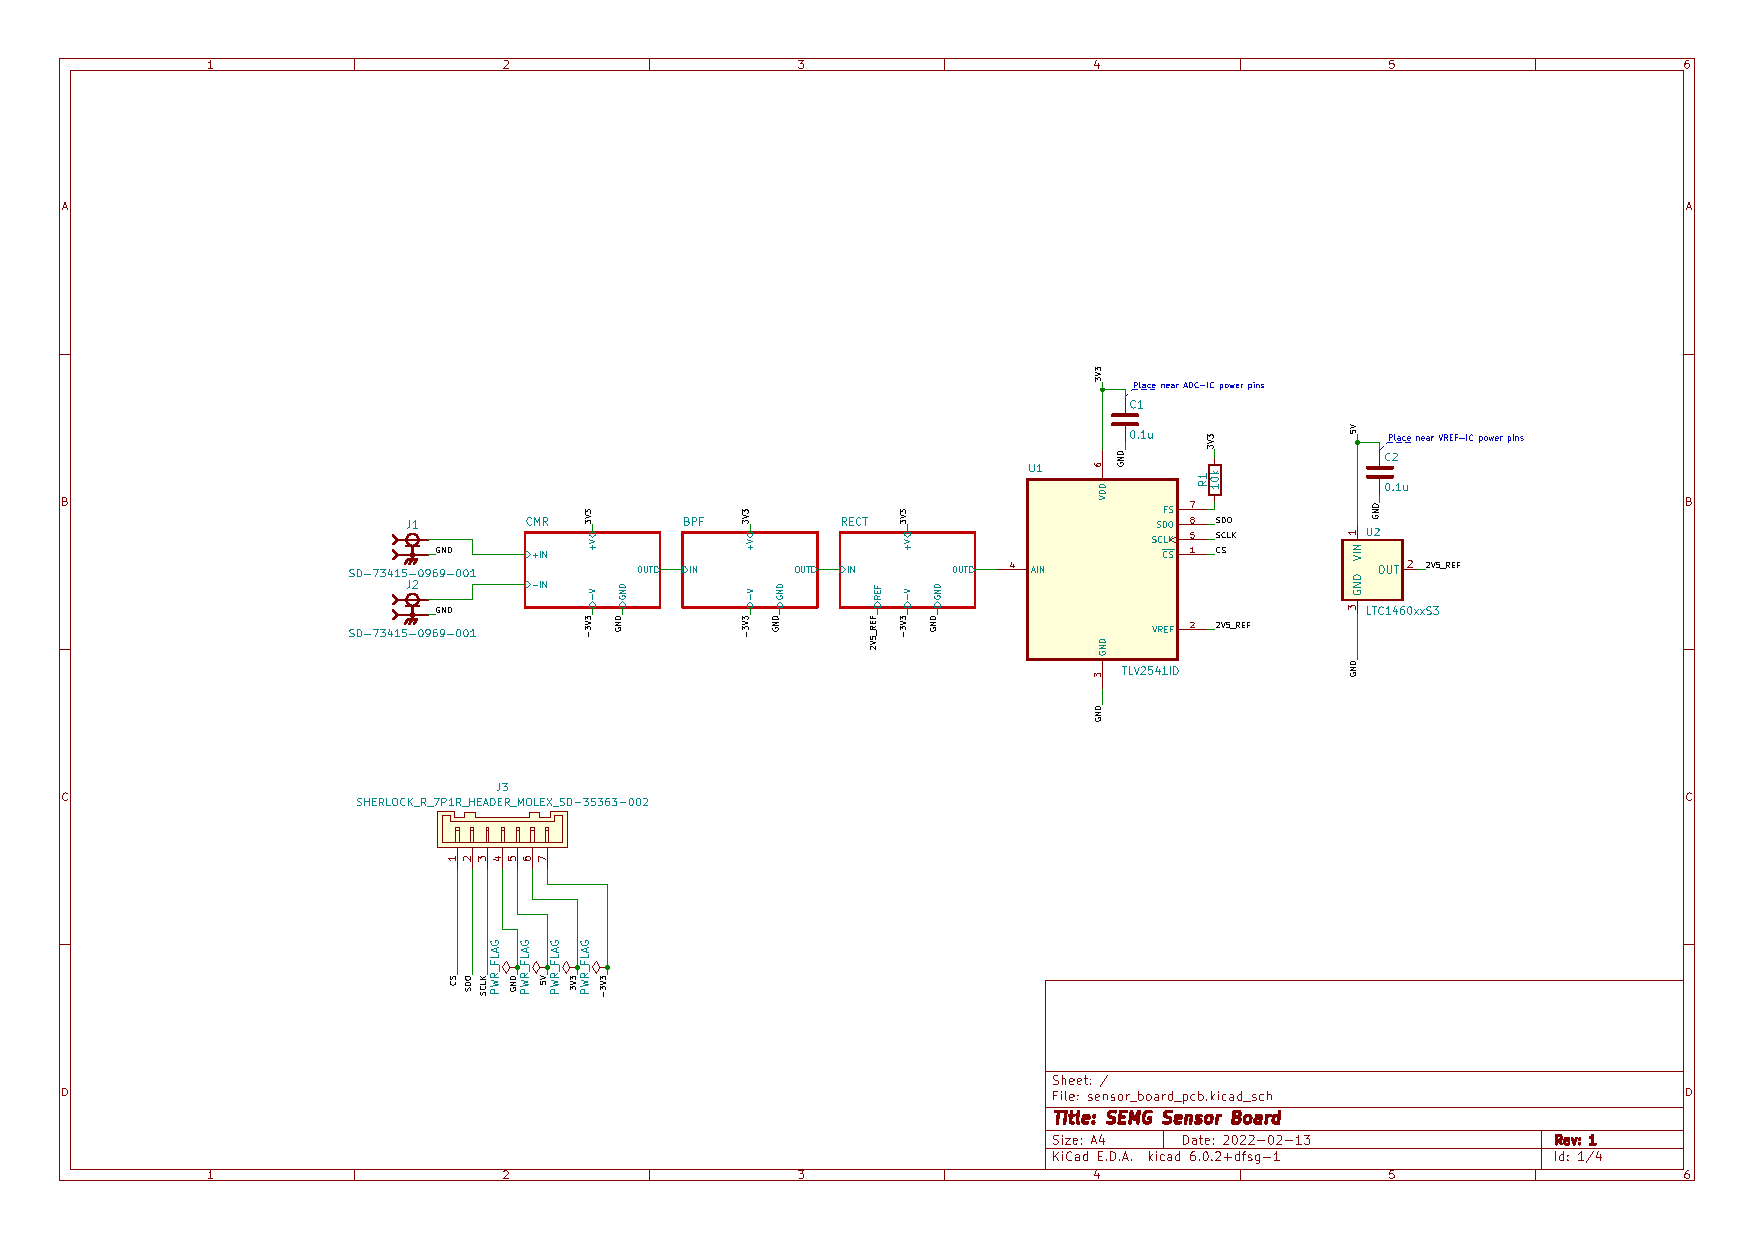
\includegraphics[height=\textwidth, angle=90]{media/sensor_board_pcb.pdf}
        \caption{Схема верхнего уровня иерархии сенсорной платы, содержащая три каскада \emph{(CMR, BPF, RECT)}, показанные на следующих рисунках \ref{fig:CircuitDiagramSensorBoardCMR}, \ref{fig:CircuitDiagramSensorBoardBPF}, \ref{fig:CircuitDiagramSensorBoardRECT}, и АЦП}
        \label{fig:CircuitDiagramSensorBoard}
    \end{figure}
    \begin{figure}[H]
        \begin{minipage}[H]{\linewidth}
            \centering
            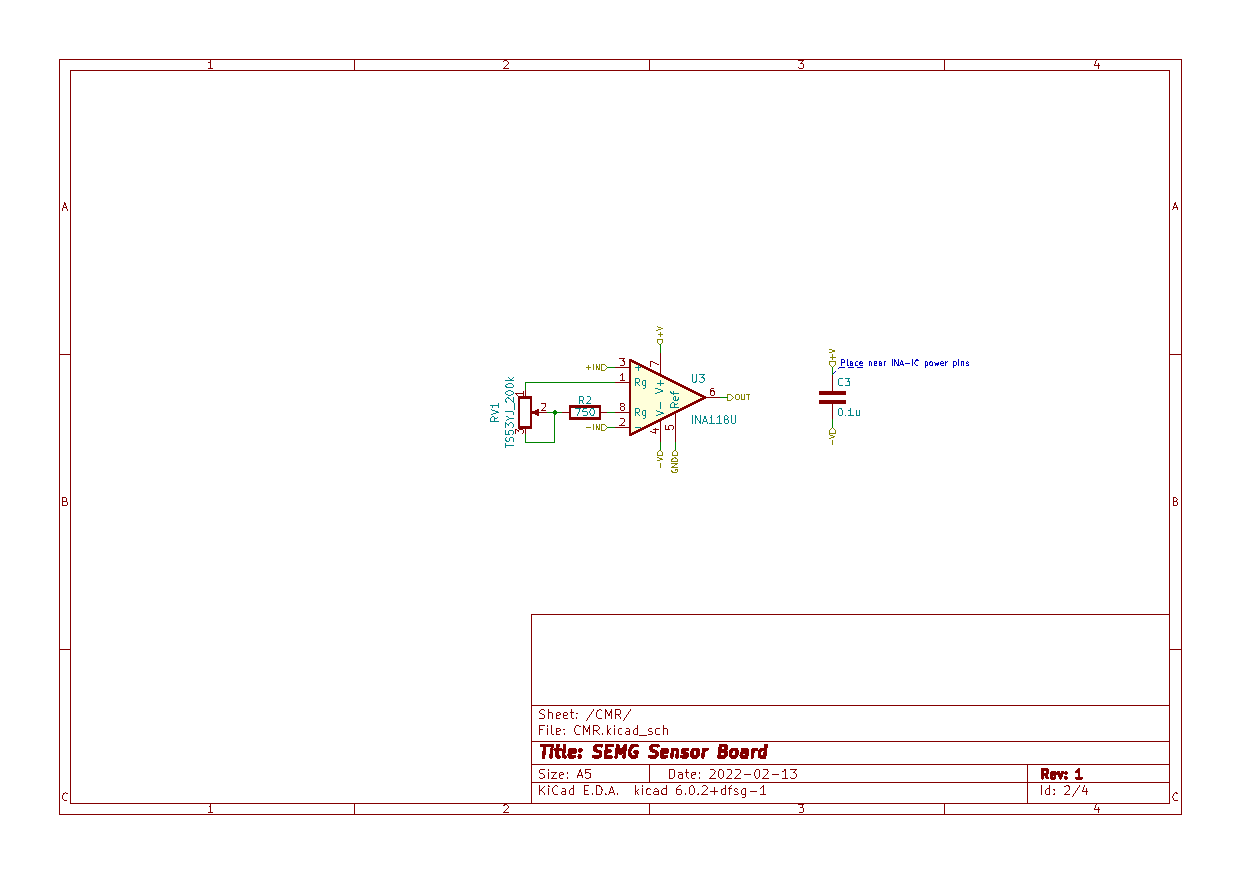
\includegraphics[width=\textwidth]{media/sensor_board_pcb-CMR.pdf}
            \subcaption{Схема на INA, фильтрующая сигнал: выделяет различающиеся части сигнала и ослабляет одинаковые}
            \label{fig:CircuitDiagramSensorBoardCMR}
        \end{minipage}
        \begin{minipage}[H]{\linewidth}
            \centering
            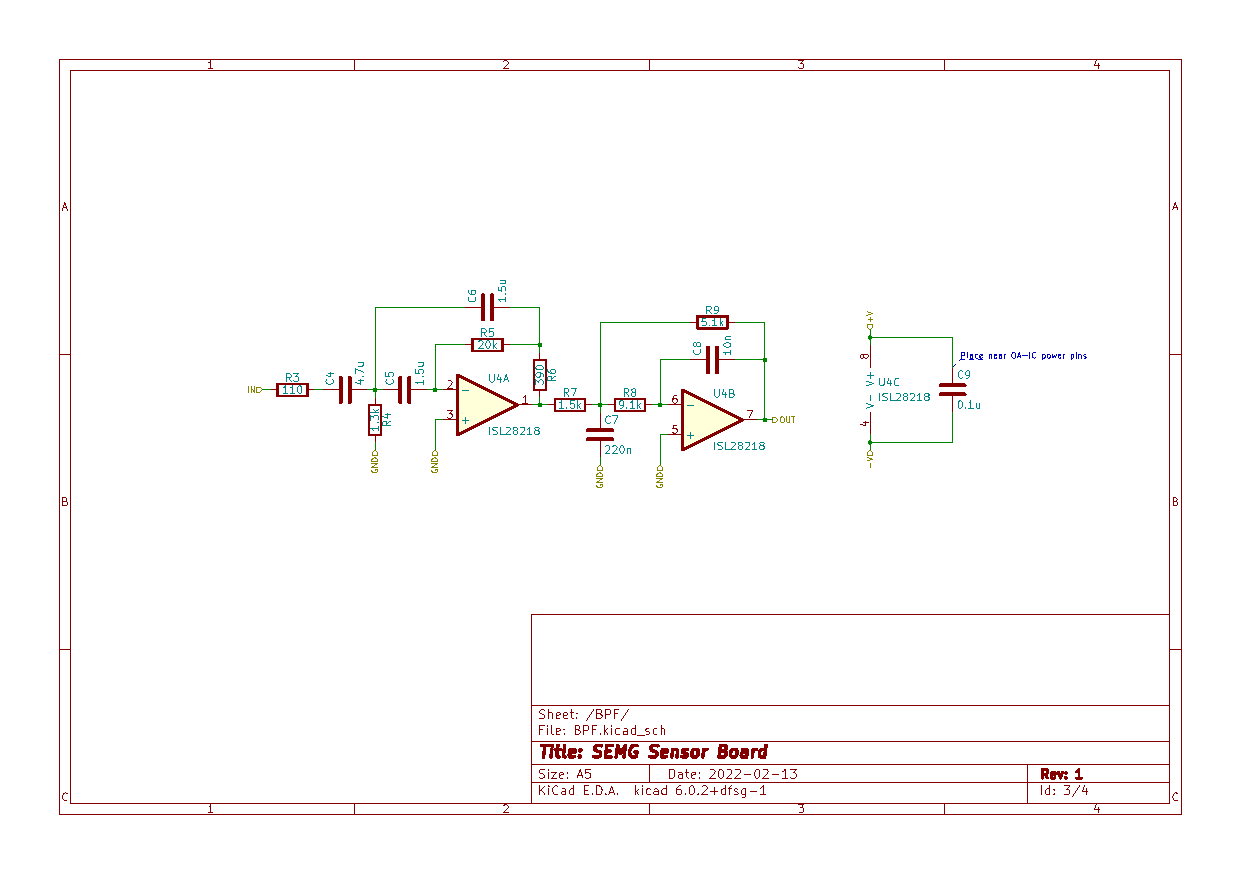
\includegraphics[width=\textwidth]{media/sensor_board_pcb-BPF.pdf}
            \subcaption{Схема из ФВЧ и ФНЧ топологии MFB для выделения полосы сигнала $20-500Hz$  \emph{(схема дважды инвертирует сигнал)}}
            \label{fig:CircuitDiagramSensorBoardBPF}
        \end{minipage}
        \caption{}
        \label{fig:CircuitDiagramSensorBoardCMRBPF}
    \end{figure}
    \begin{figure}[H]
        \centering
        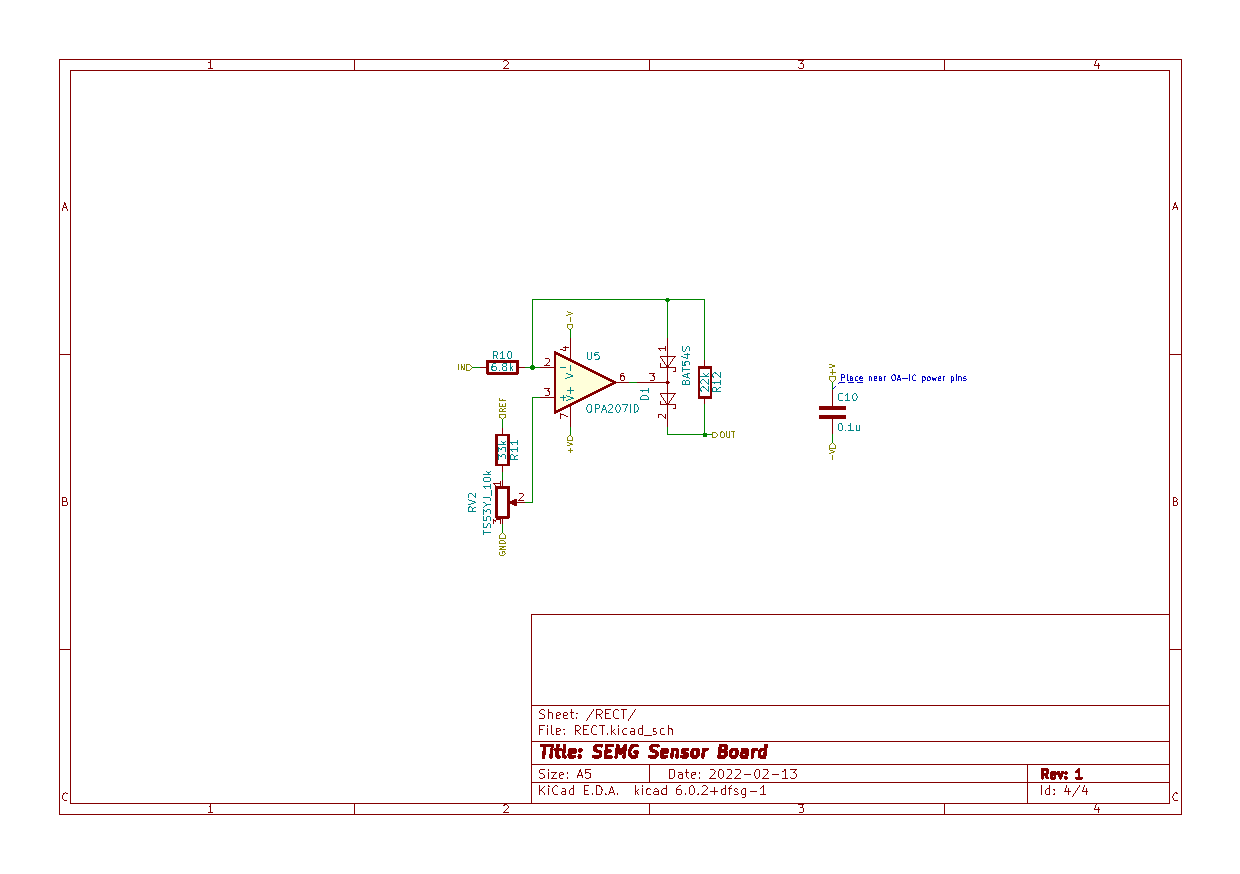
\includegraphics[width=\textwidth]{media/sensor_board_pcb-RECT.pdf}
        \caption{Схема выпрямления сигнала \emph{(в этой топологии сигнал инвертируется, а его отрицательная часть срезается)}}
        \label{fig:CircuitDiagramSensorBoardRECT}
    \end{figure}

    \noindent Приведённые схемы:
    \begin{itemize}
        \item SEMG Sensor Board --- сенсорная плата
        \item SEMG Sensor Board - CMR --- часть с INA, названная так по Common Mode Rejection, то есть подавлению синфазного сигнала
        \item SEMG Sensor Board - BPF --- часть частотной фильтрации, выделяющая полосу частот $20-500Hz$
        \item SEMG Sensor Board - RECT --- часть выпрямления сигнала\footnote{АЦП не может принимать отрицательное напряжение ниже $0.3V$ \parenciteit{p8}{TLV2541:Datasheet}}
    \end{itemize}
    Схема питается от двух источников, отрицательного и положительного; они нужны INA, чтобы задать опорное напряжение на уровне тела, и для работы с сигналом при использовании ФВЧ\footnote{Все низкочастотные составляющие и постоянная составляющая отфильтровываются, и сигнал центрируется около $0V$}.
    % TRANSLATOR NOTE: "LTO" kept as in the original; almost certainly means LDO.
    Я добавил схему «SEMG Sensor Board - RECT», чтобы не выходить за пределы напряжения АЦП, хотя сигнал можно центрировать около значения в диапазоне $2.5-0V$\footnote{$2.5V$ обеспечивает фиксированный стабилизатор LTO на $2.5V$ $U2$}, задаваемого потенциометром $RV2$.
    Амплитуда сигнала регулируется потенциометром $RV1$\footnote{В последний момент я обнаружил, что рассчитанные мной значения усиления были неточны, и изменил номинал резистора $R2$ с $10k\Omega$ на $750\Omega$, тем самым увеличив максимальный коэффициент усиления схемы}.
    Другие заметные изменения по сравнению с концептуальной схемой, предложенной в большей части раздела \ref{sec:FilterTheory}, --- резисторы $R3$ и $R6$\footnote{Резисторов два, чтобы не изменять передаточную функцию}\:\footnote{Номиналы этих резисторов получены подбором (методом проб) при моделировании в KiCad}, которые ограничивают максимальный ток, который может течь с выхода усилителя $U4A$ или INA $U3$ на очень высоких частотах, снижающих импеданс конденсаторов $C6$ и $C4$, что могло бы привести к сбою $U3$ или $U4A$.
    Кроме того, заметны конденсаторы $C1$, $C2$, $C3$, $C9$ и $C10$, у которых есть собственное название --- блокировочные (bypass capacitors); их функция --- подавлять высокочастотные шумы в линиях питания, которые могут приходить от цифровой части схемы\footnote{Не только от АЦП, но и со стороны источника питания, подключаемого через разъём $J3$}.
    У АЦП три вывода, служащие для передачи информации по протоколу SPI; они подключены к разъёму $J3$.
    Два других разъёма, $J1$ и $J2$, служат для подключения кабелей электродов\footnote{Они соединены с GND, поскольку кабель электродов экранирован для уменьшения помех и поскольку у электродов два контакта: опорный и сигнальный}
    $R1$ --- формальность, предписанная технической документацией АЦП\footcite[p5,p21]{TLV2541:Datasheet}, чтобы указать ему, в каком режиме работать.

    \subsubsection{Выбор компонентов}
    Имея формулы фильтров и данные из технической документации компонентов, я подобрал\footnote{Выбор компонентов всегда выполнялся итеративным «modus operandi» с помощью базы данных компонентов выбранного дистрибьютора \parencite[]{Mouser:Web}} пассивные компоненты методом проб, чтобы сбалансировать различные факторы, такие как шумы\footnote{В расчётах в разделе \ref{sec:Calculations} я использовал только компоненты с данными об их белом шуме (одинаковом по всему спектру) и розовом, или фликкер-шуме (более выраженном на низких частотах)}, генерируемые схемой.

    Затем я начал моделировать схему, чтобы получить номиналы пассивных компонентов из стандартных рядов E, по возможности одинаковые, чтобы сократить BOM\footnote{Bill of Materials --- перечень компонентов, которые нужно закупить, чтобы собрать схему}, но без компромиссов в заданных параметрах\footnote{Усиление, частоты среза фильтров и шумы компонентов (величина шумов определена в расчётах раздела \ref{sec:Calculations})}.

    \begin{figure}[H]
        \centering
        \begin{minipage}[H]{\linewidth}
            \centering
            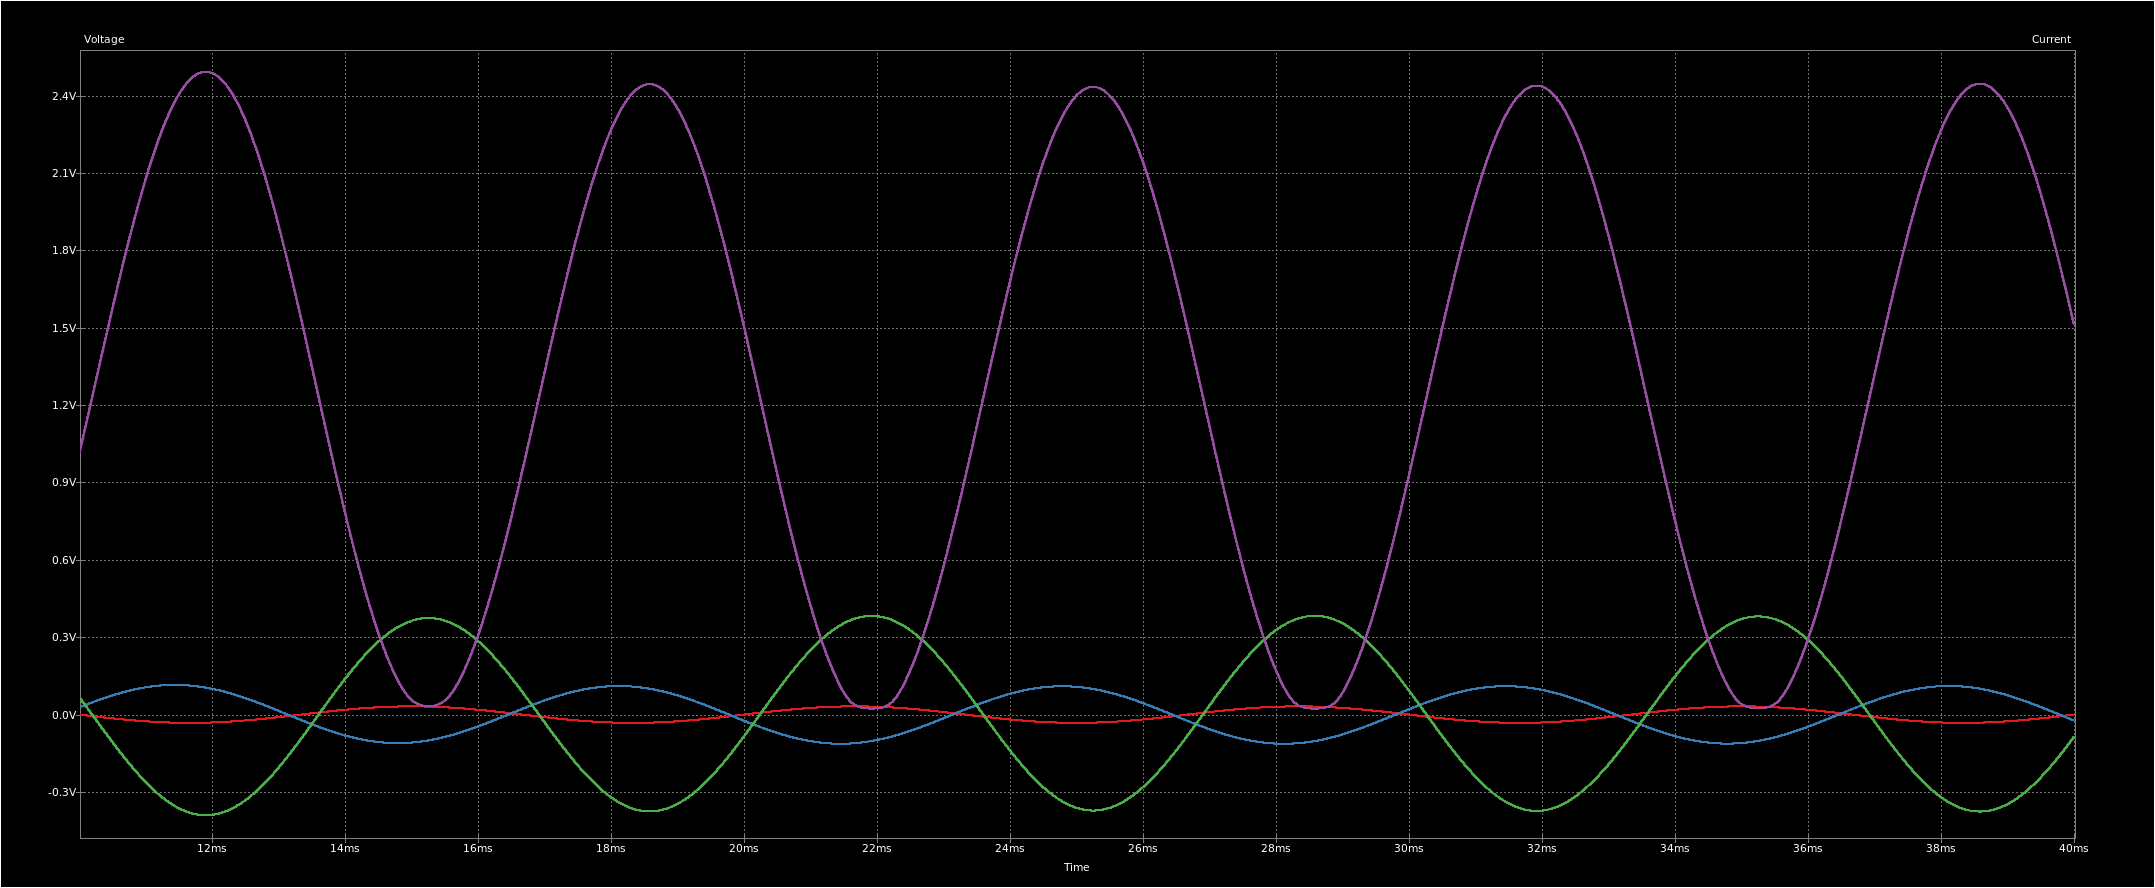
\includegraphics[width=\linewidth]{media/simtimeresp.png}
            \subcaption{Временной отклик схемы при моделировании: красный сигнал --- на выходе каскада гипотетического INA \emph{($SIG\_IN$)}, синий --- на выходе ФВЧ \emph{(выход $U1$)}, зелёный --- на выходе ФНЧ \emph{(выход $U2$)}, фиолетовый --- на выходе выпрямителя \emph{($SIG\_OUT$)} \emph{(в данном случае входной сигнал каскада частотных фильтров --- $32mV$ с частотой $150Hz$, центрированный на последнем каскаде около $1.25V$)}}
            \label{fig:timeresp}
        \end{minipage}
        \\
        \begin{minipage}[H]{\linewidth}
            \centering
            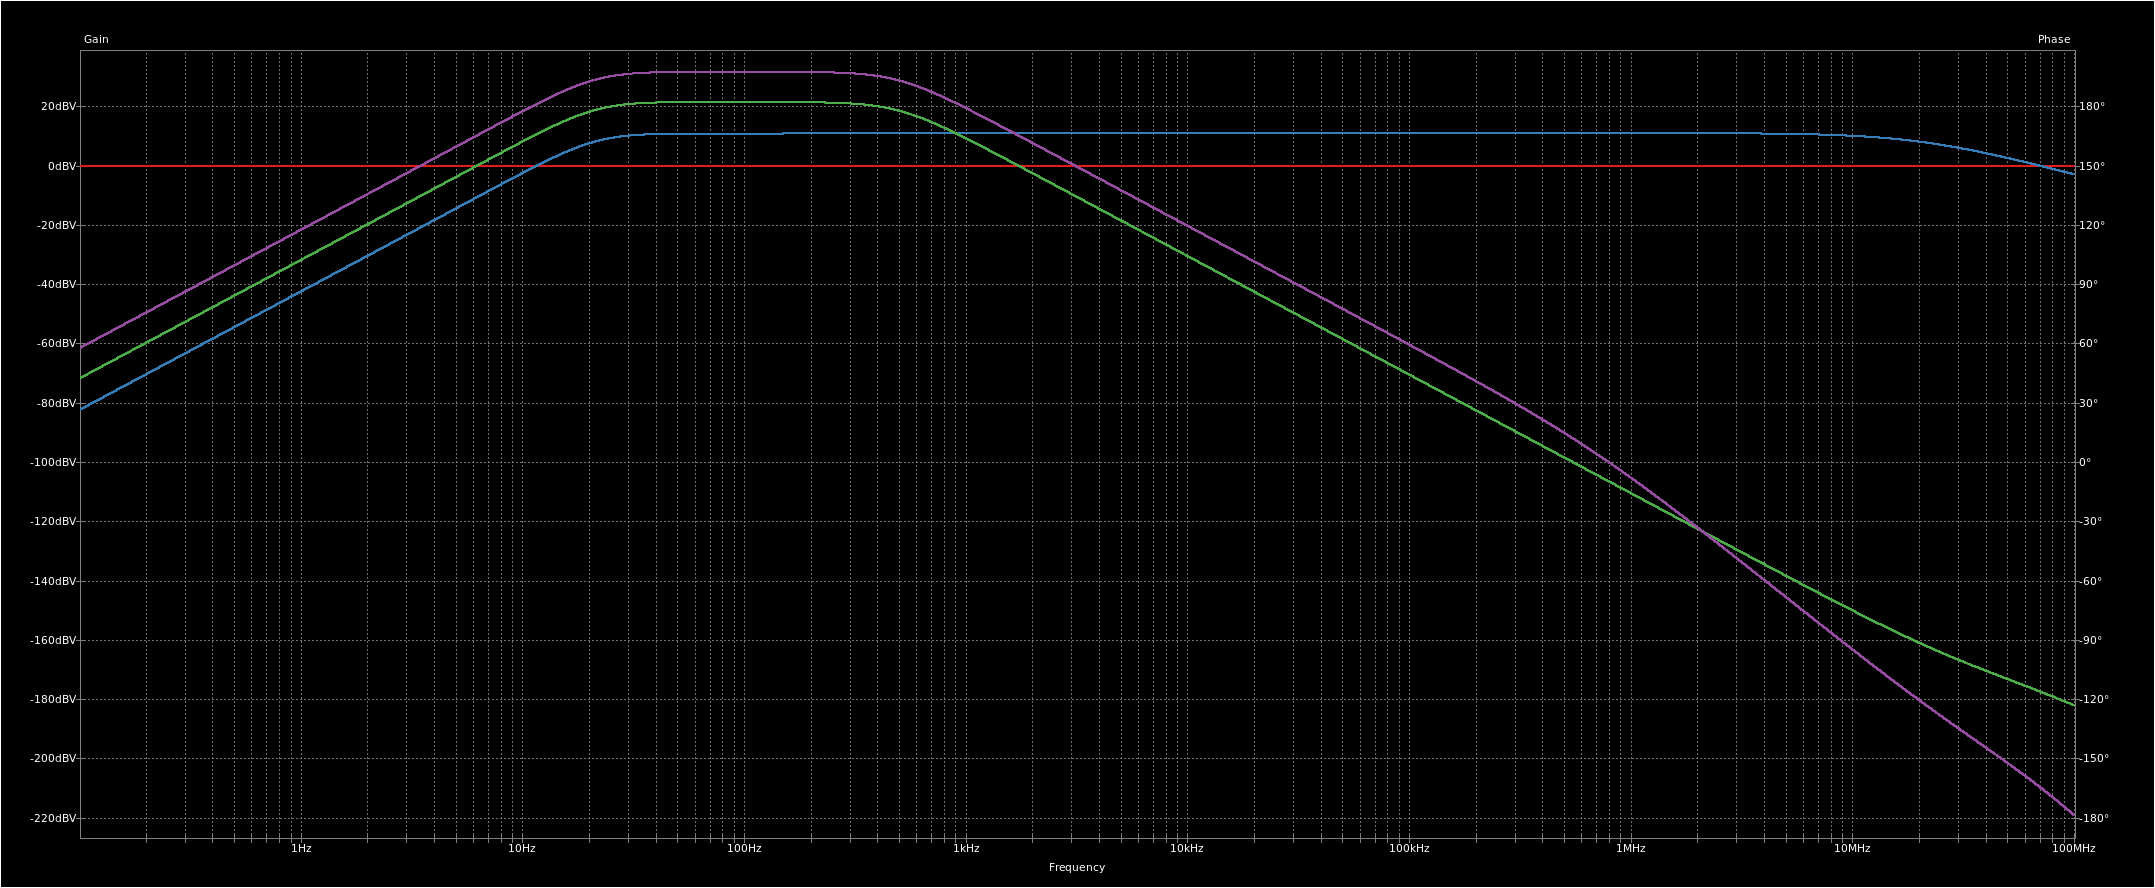
\includegraphics[width=\linewidth]{media/simfreqresp.png}
            \subcaption{Частотная характеристика схемы: красный сигнал --- на выходе гипотетического INA \emph{($SIG\_IN$)}, синий --- на выходе ФВЧ \emph{(выход $U1$)}, зелёный --- на выходе ФНЧ \emph{(выход $U2$)}, фиолетовый --- на выходе выпрямителя \emph{($SIG\_OUT$)}}
            \label{fig:freqresp}
        \end{minipage}
        \caption{Графики, описывающие поведение фильтра при моделировании}
        \label{fig:freqtimeresp}
    \end{figure}

    \begin{figure}[H]
        \centering
        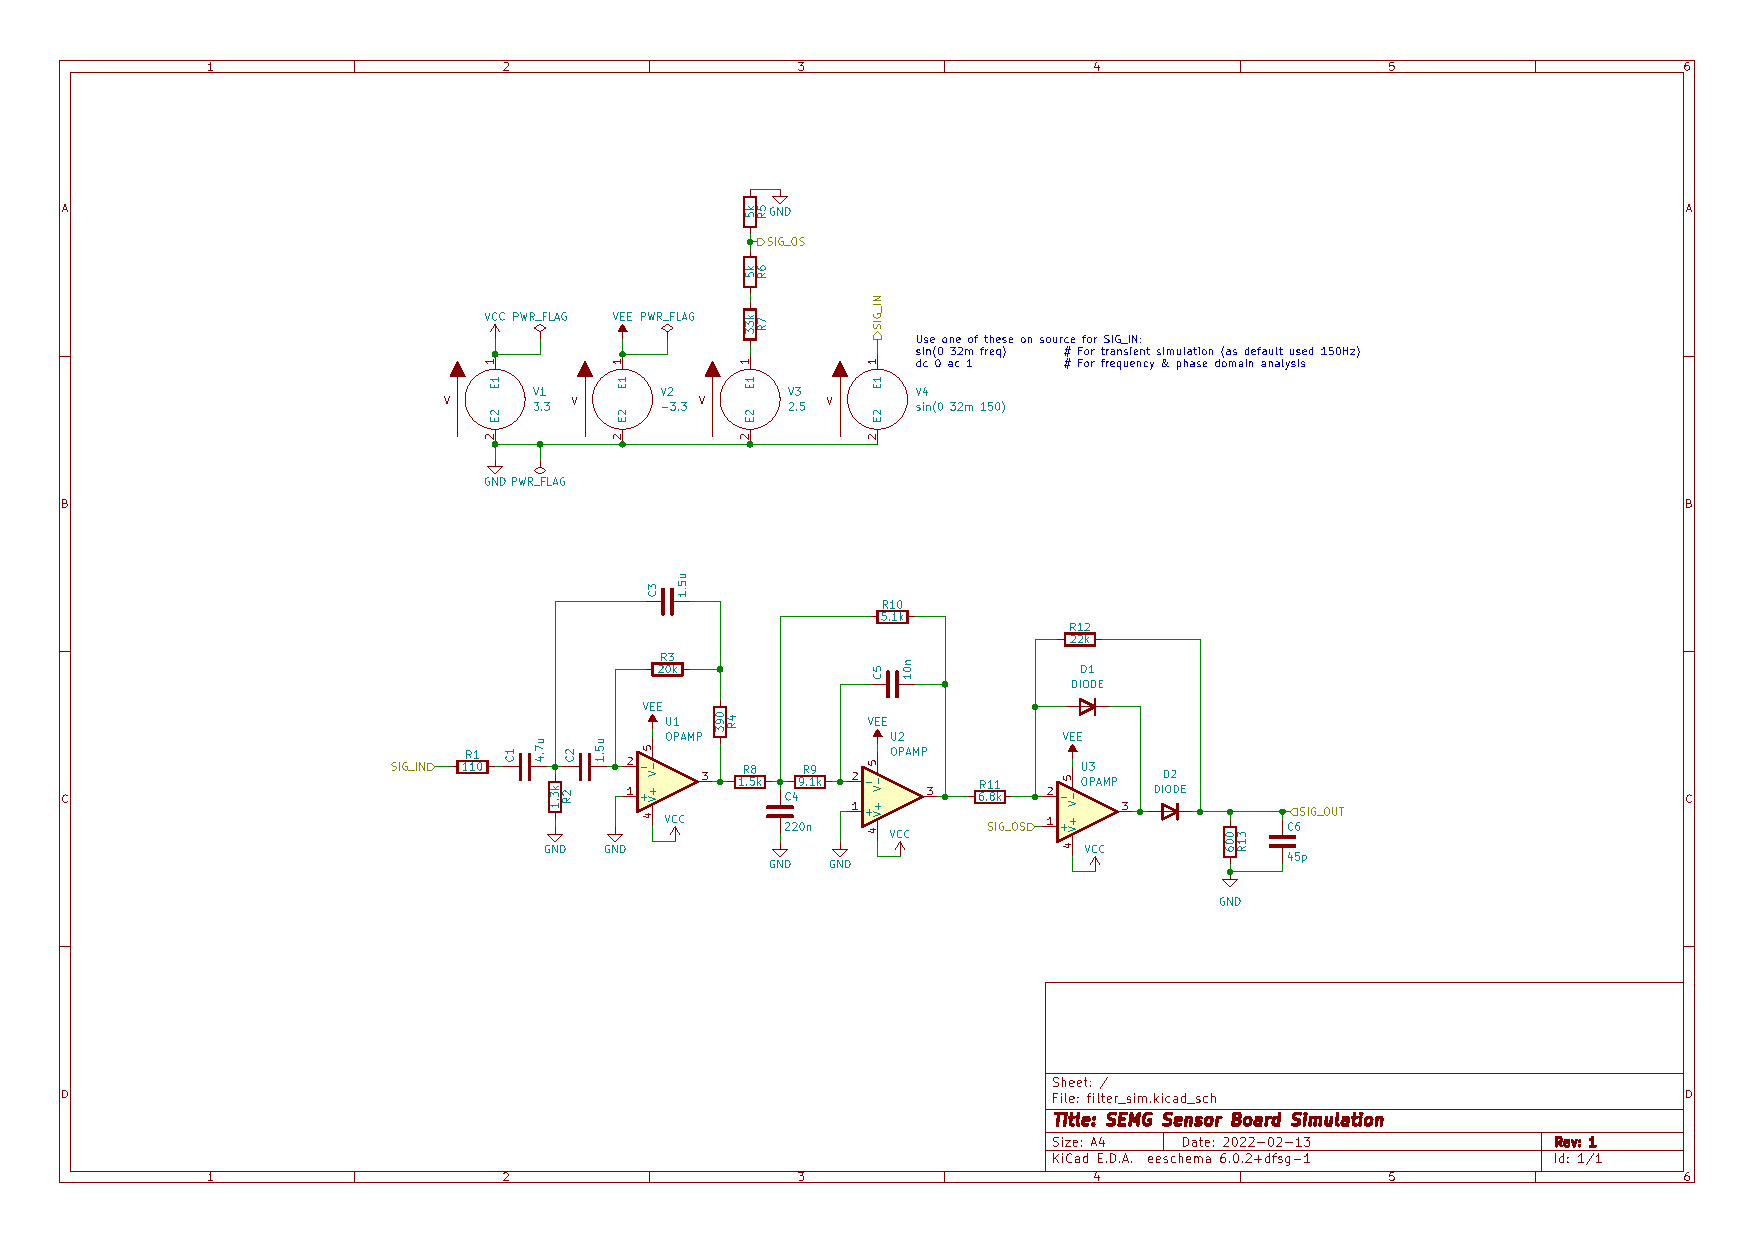
\includegraphics[height=\textwidth, angle=90]{media/filter_sim.pdf}
        \caption{Схема, на которой проводилось моделирование}
    \end{figure}

    \noindent Прежде всего я выбрал АЦП, подходящий для логического уровня $3.3V$ и с разрешением $12bit$\footnote{С отношением сигнал/шум (SNR, Signal to Noise Ratio --- отношение мощности сигнала к мощности шума) около $72dB$, поскольку это само разрешение, выраженное в $[dB]$, что рассчитано в разделе \ref{sec:Calculations}}.
    \todo{Дать более подробные ссылки на расчёты (на отдельные файлы)}

    % TRANSLATOR NOTE: the GBPW footnote is unfinished in the original ("Gain Bandwidth Power, oppure "); translated as-is. Standard term: Gain-Bandwidth Product (GBW).
    Чтобы выбрать активные компоненты\footnote{Имеются в виду микросхемы, обозначенные $UX$ на схемах на рисунках \ref{fig:CircuitDiagramSensorBoard} \ref{fig:CircuitDiagramSensorBoardCMRBPF} \ref{fig:CircuitDiagramSensorBoardRECT}} аналоговой части, я постарался рассчитать минимумы и максимумы различных характеристик каждого компонента, таких как GBPW\footnote{Gain Bandwidth Power, или }, скорость нарастания (slew rate)\footnote{Скорость реакции усилителя, то есть насколько может измениться его напряжение за определённый интервал времени (измеряется в $[V/\mu s]$)}, максимальные выходные токи и другие\footnote{Их можно увидеть в разделе \ref{sec:Calculations}}, для ОУ и INA, чтобы согласовать их с выбранным АЦП

    \subsubsection{Разводка платы}
    Для разводки\footnote{Размещение компонентов и дорожек, которые будут служить проводниками} платы я выбрал однотипные корпуса компонентов: все микросхемы --- в корпусе SOIC-8\footcite[]{SOIC:Wiki}, диоды и источник опорного напряжения --- в корпусе SOT-223\footcite[]{SOT:Wiki}, а пассивные компоненты --- типоразмера 1608\footnote{В метрической системе}\:\footcite[]{SMT:Wiki}, чтобы их было удобно паять паяльником, не жертвуя малым размером схемы.

    Разумеется, для платы я выбрал вариант с наименьшим возможным числом слоёв, чтобы уменьшить сложность схемы и иметь возможность изготовить её дома методом утюга\footnote{Об этом рассказывается в разделе \ref{sec:BuildingHardware}} и химического травления\footnote{Об этом рассказывается в разделе \ref{sec:BuildingHardware}}.
    Кроме того, я отвёл нижний слой под GND, чтобы улучшить развязку (decoupling)\footnote{Все компоненты вносят шумы и в питание, когда потребляют разный ток в разные моменты времени} компонентов, как того требует хорошая практика.

    Ширина дорожек выбрана произвольно\footnote{Вкладом скин-эффекта \parenciteit{}{SkinEffect:Wiki} можно пренебречь на низких частотах, таких как те, с которыми мы работаем}

    \begin{figure}[H]
        \centering
        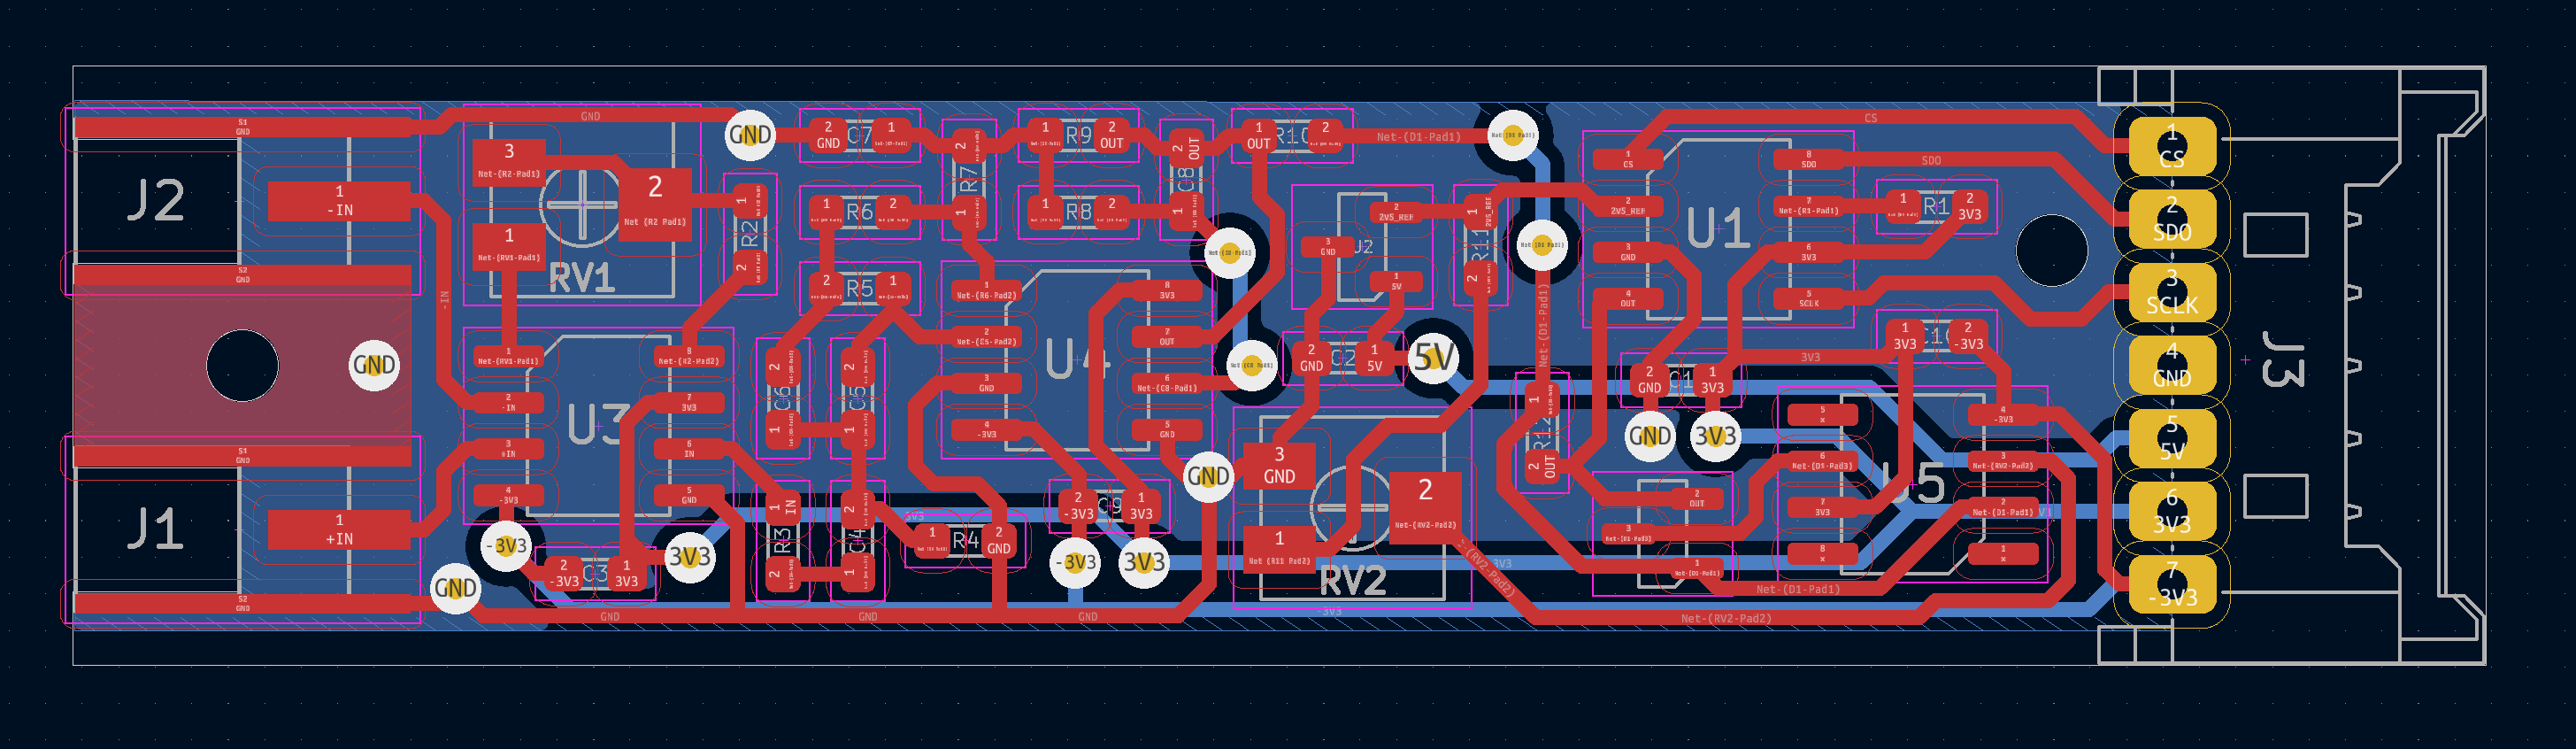
\includegraphics[width=\linewidth]{media/Layout.png}
        \caption{Разводка сенсорной платы: нижний проводящий слой платы показан синим, верхний --- красным, переходные отверстия --- жёлто-белыми кружками}
        \label{fig:Layout}
    \end{figure}
    \clearpage

    \section{Изготовление}\label{sec:Building}
    \subsection{Аппаратная часть}\label{sec:BuildingHardware}
    Сначала я распечатал на листах офисной бумаги несколько вариантов схемы\footnote{Рисунок \ref{fig:BuildingHardwarePaperSheet}}.
    \begin{figure}[H]
        \centering
        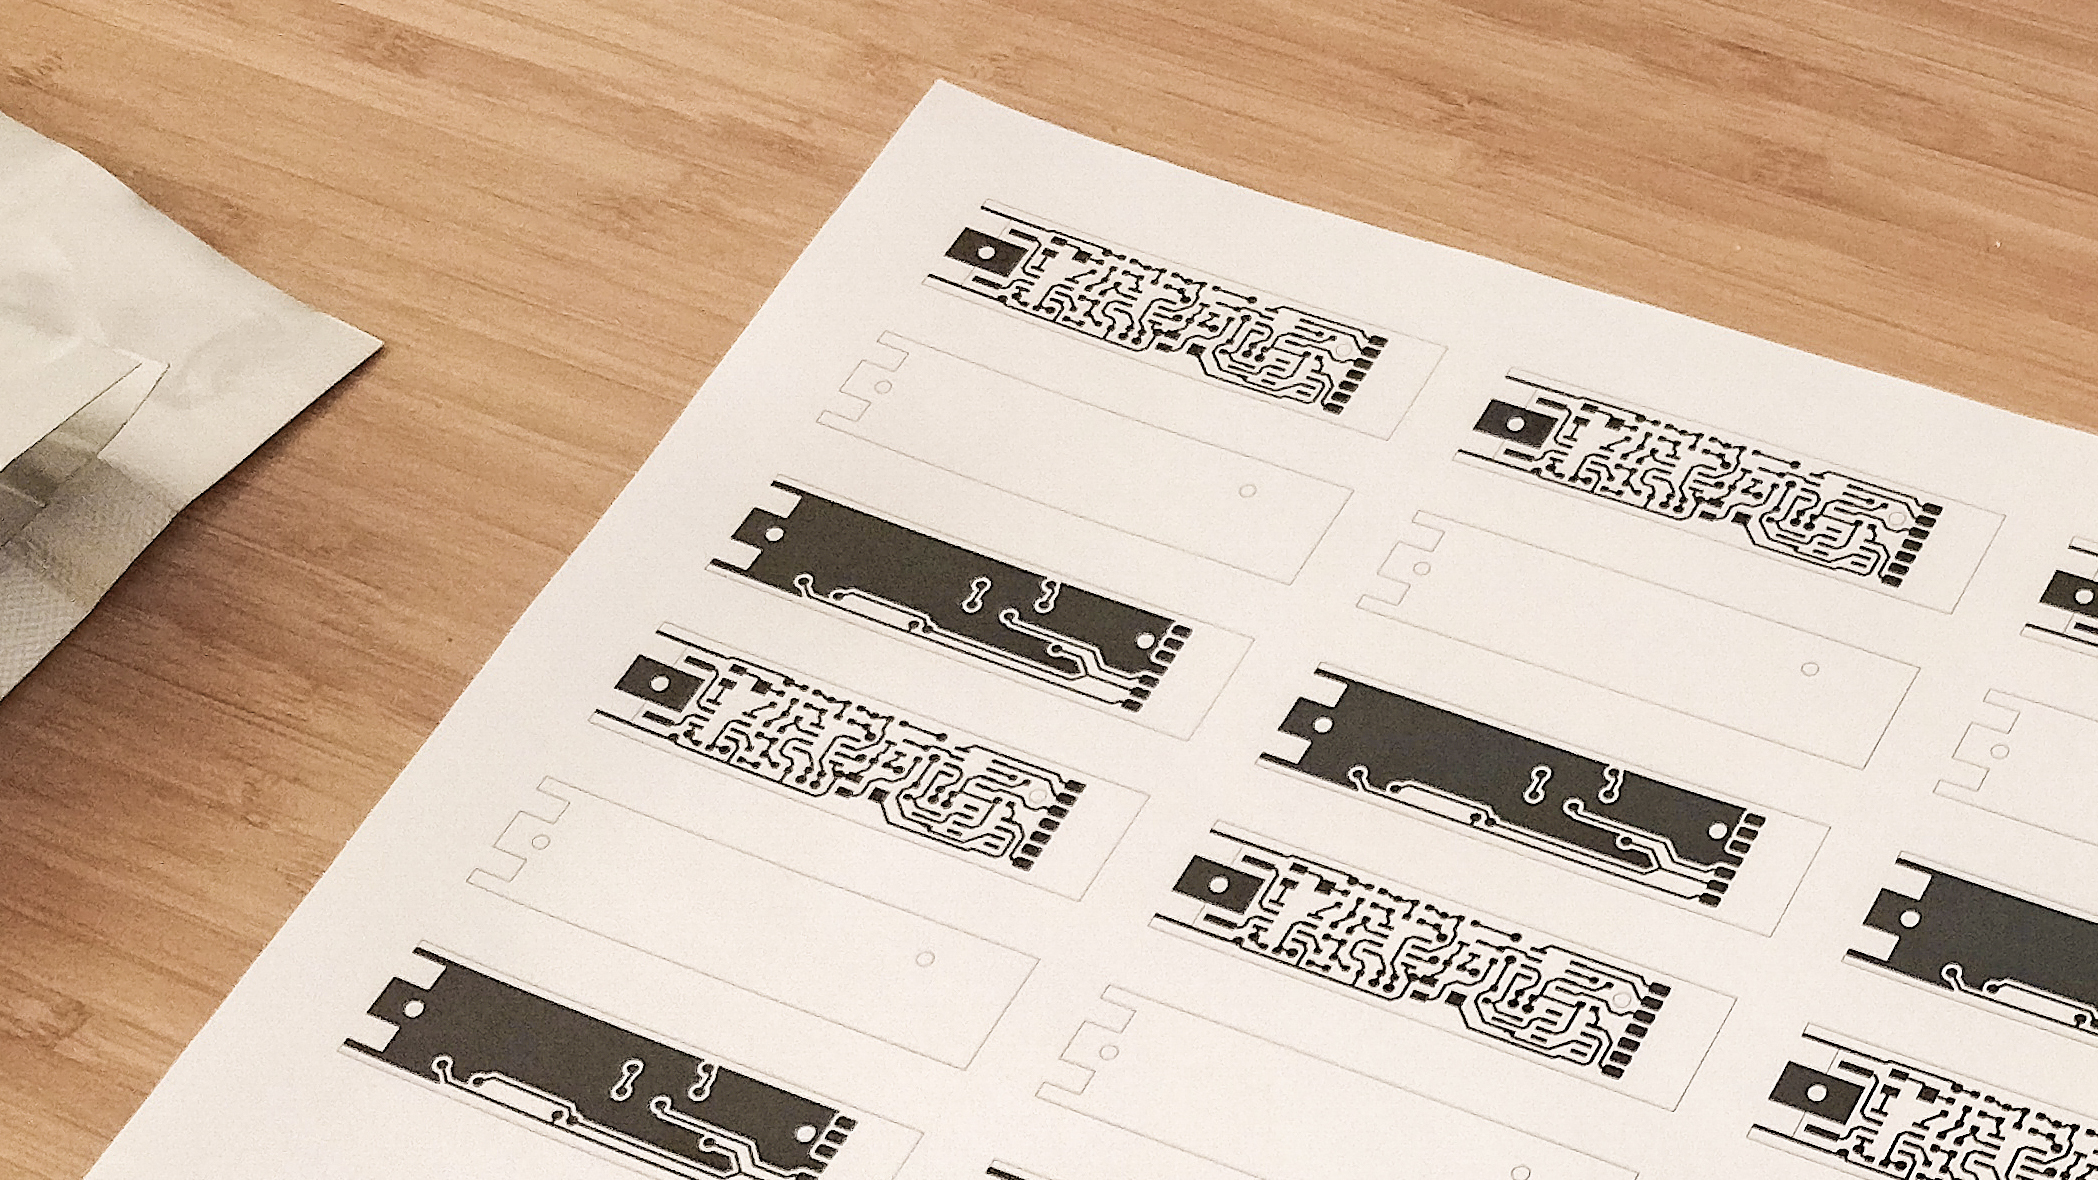
\includegraphics[width=.95\linewidth]{media/album/PSX_20220228_025610.jpg}
        \caption{}
        \label{fig:BuildingHardwarePaperSheet}
    \end{figure}
    Затем я отобрал лучше всего получившиеся варианты и отложил их, чтобы использовать как маски для химического травления, а неудачные использовал как шаблон для подготовки заготовки платы\footnote{Рисунок \ref{fig:PhotoPCBCut}}.
    Подготовка заключалась в сверлении отверстий\footnote{Рисунок \ref{fig:PhotoPCBDrill}} в определённых местах для переходных отверстий\footnote{Соединения между слоями платы, которые я сделал самым простым способом: отверстие и жилка провода} и последующей очистке поверхности платы.

    \begin{figure}[H]
        \centering
        \begin{minipage}[H]{.45\linewidth}
            \centering
            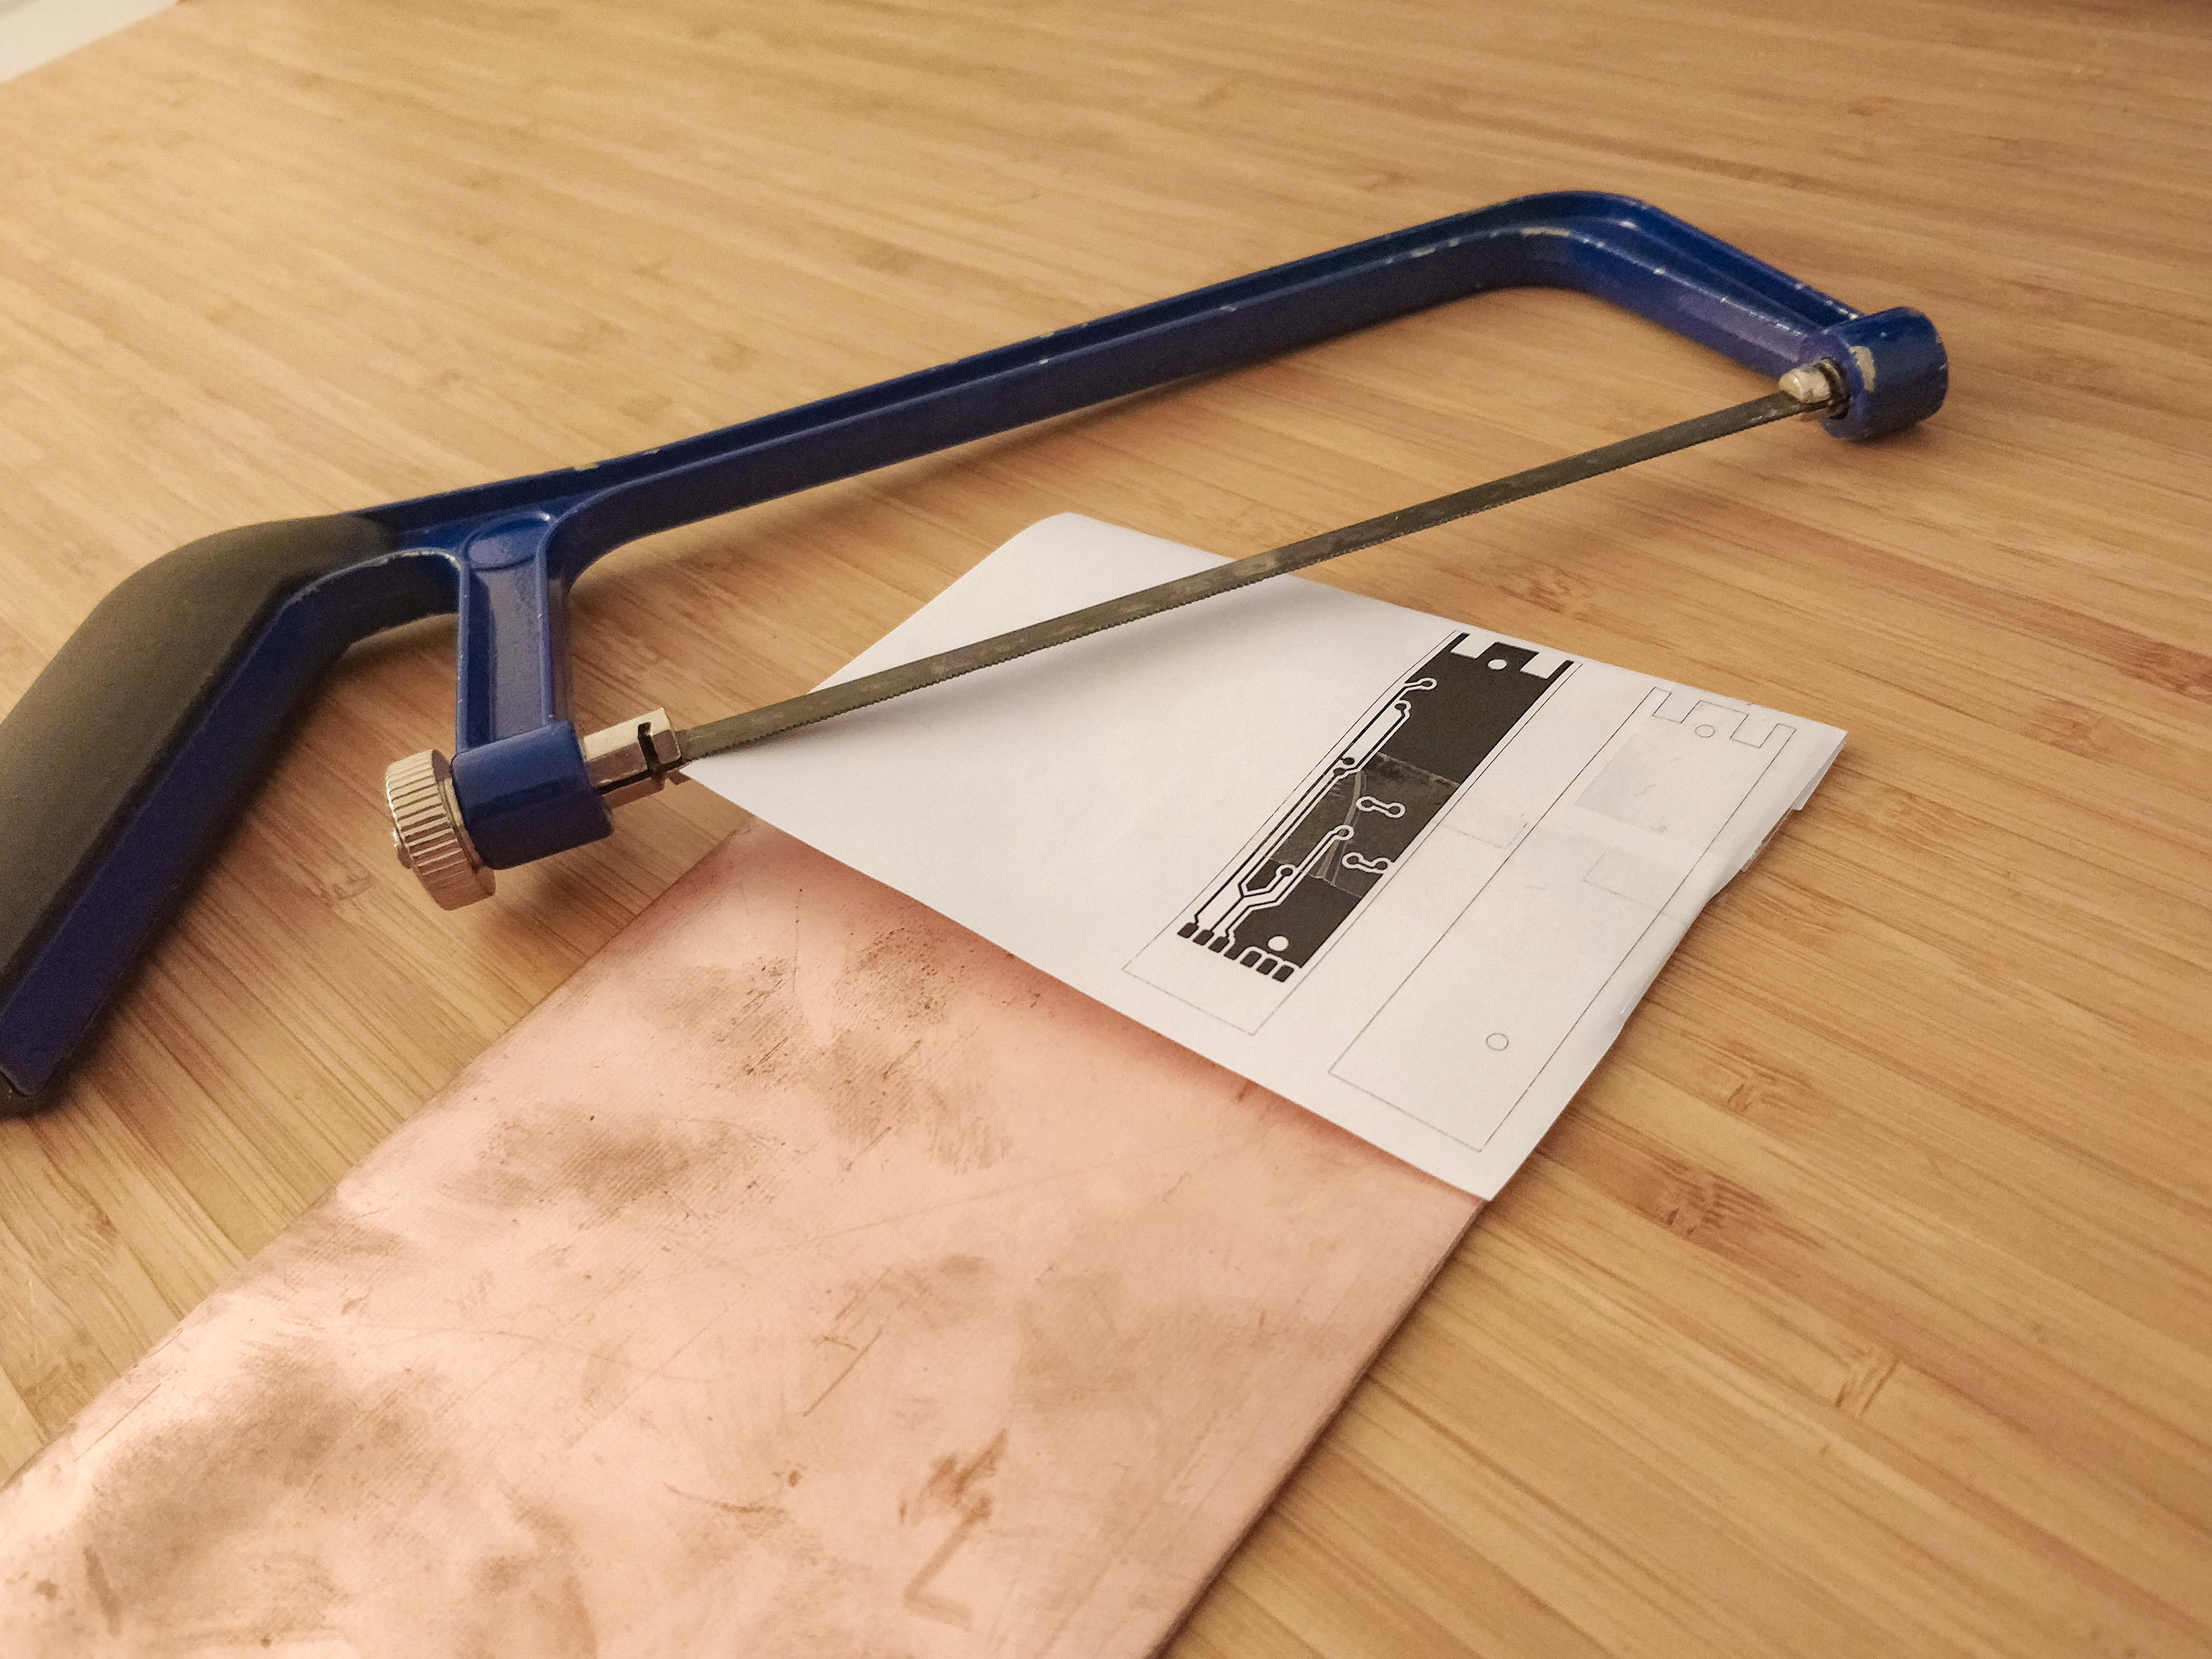
\includegraphics[width=\linewidth]{media/album/PSX_20220228_025933.jpg}
            \caption{}
            \label{fig:PhotoPCBCut}
        \end{minipage}
        \hspace{.04\linewidth}
        \begin{minipage}[H]{.45\linewidth}
            \centering
            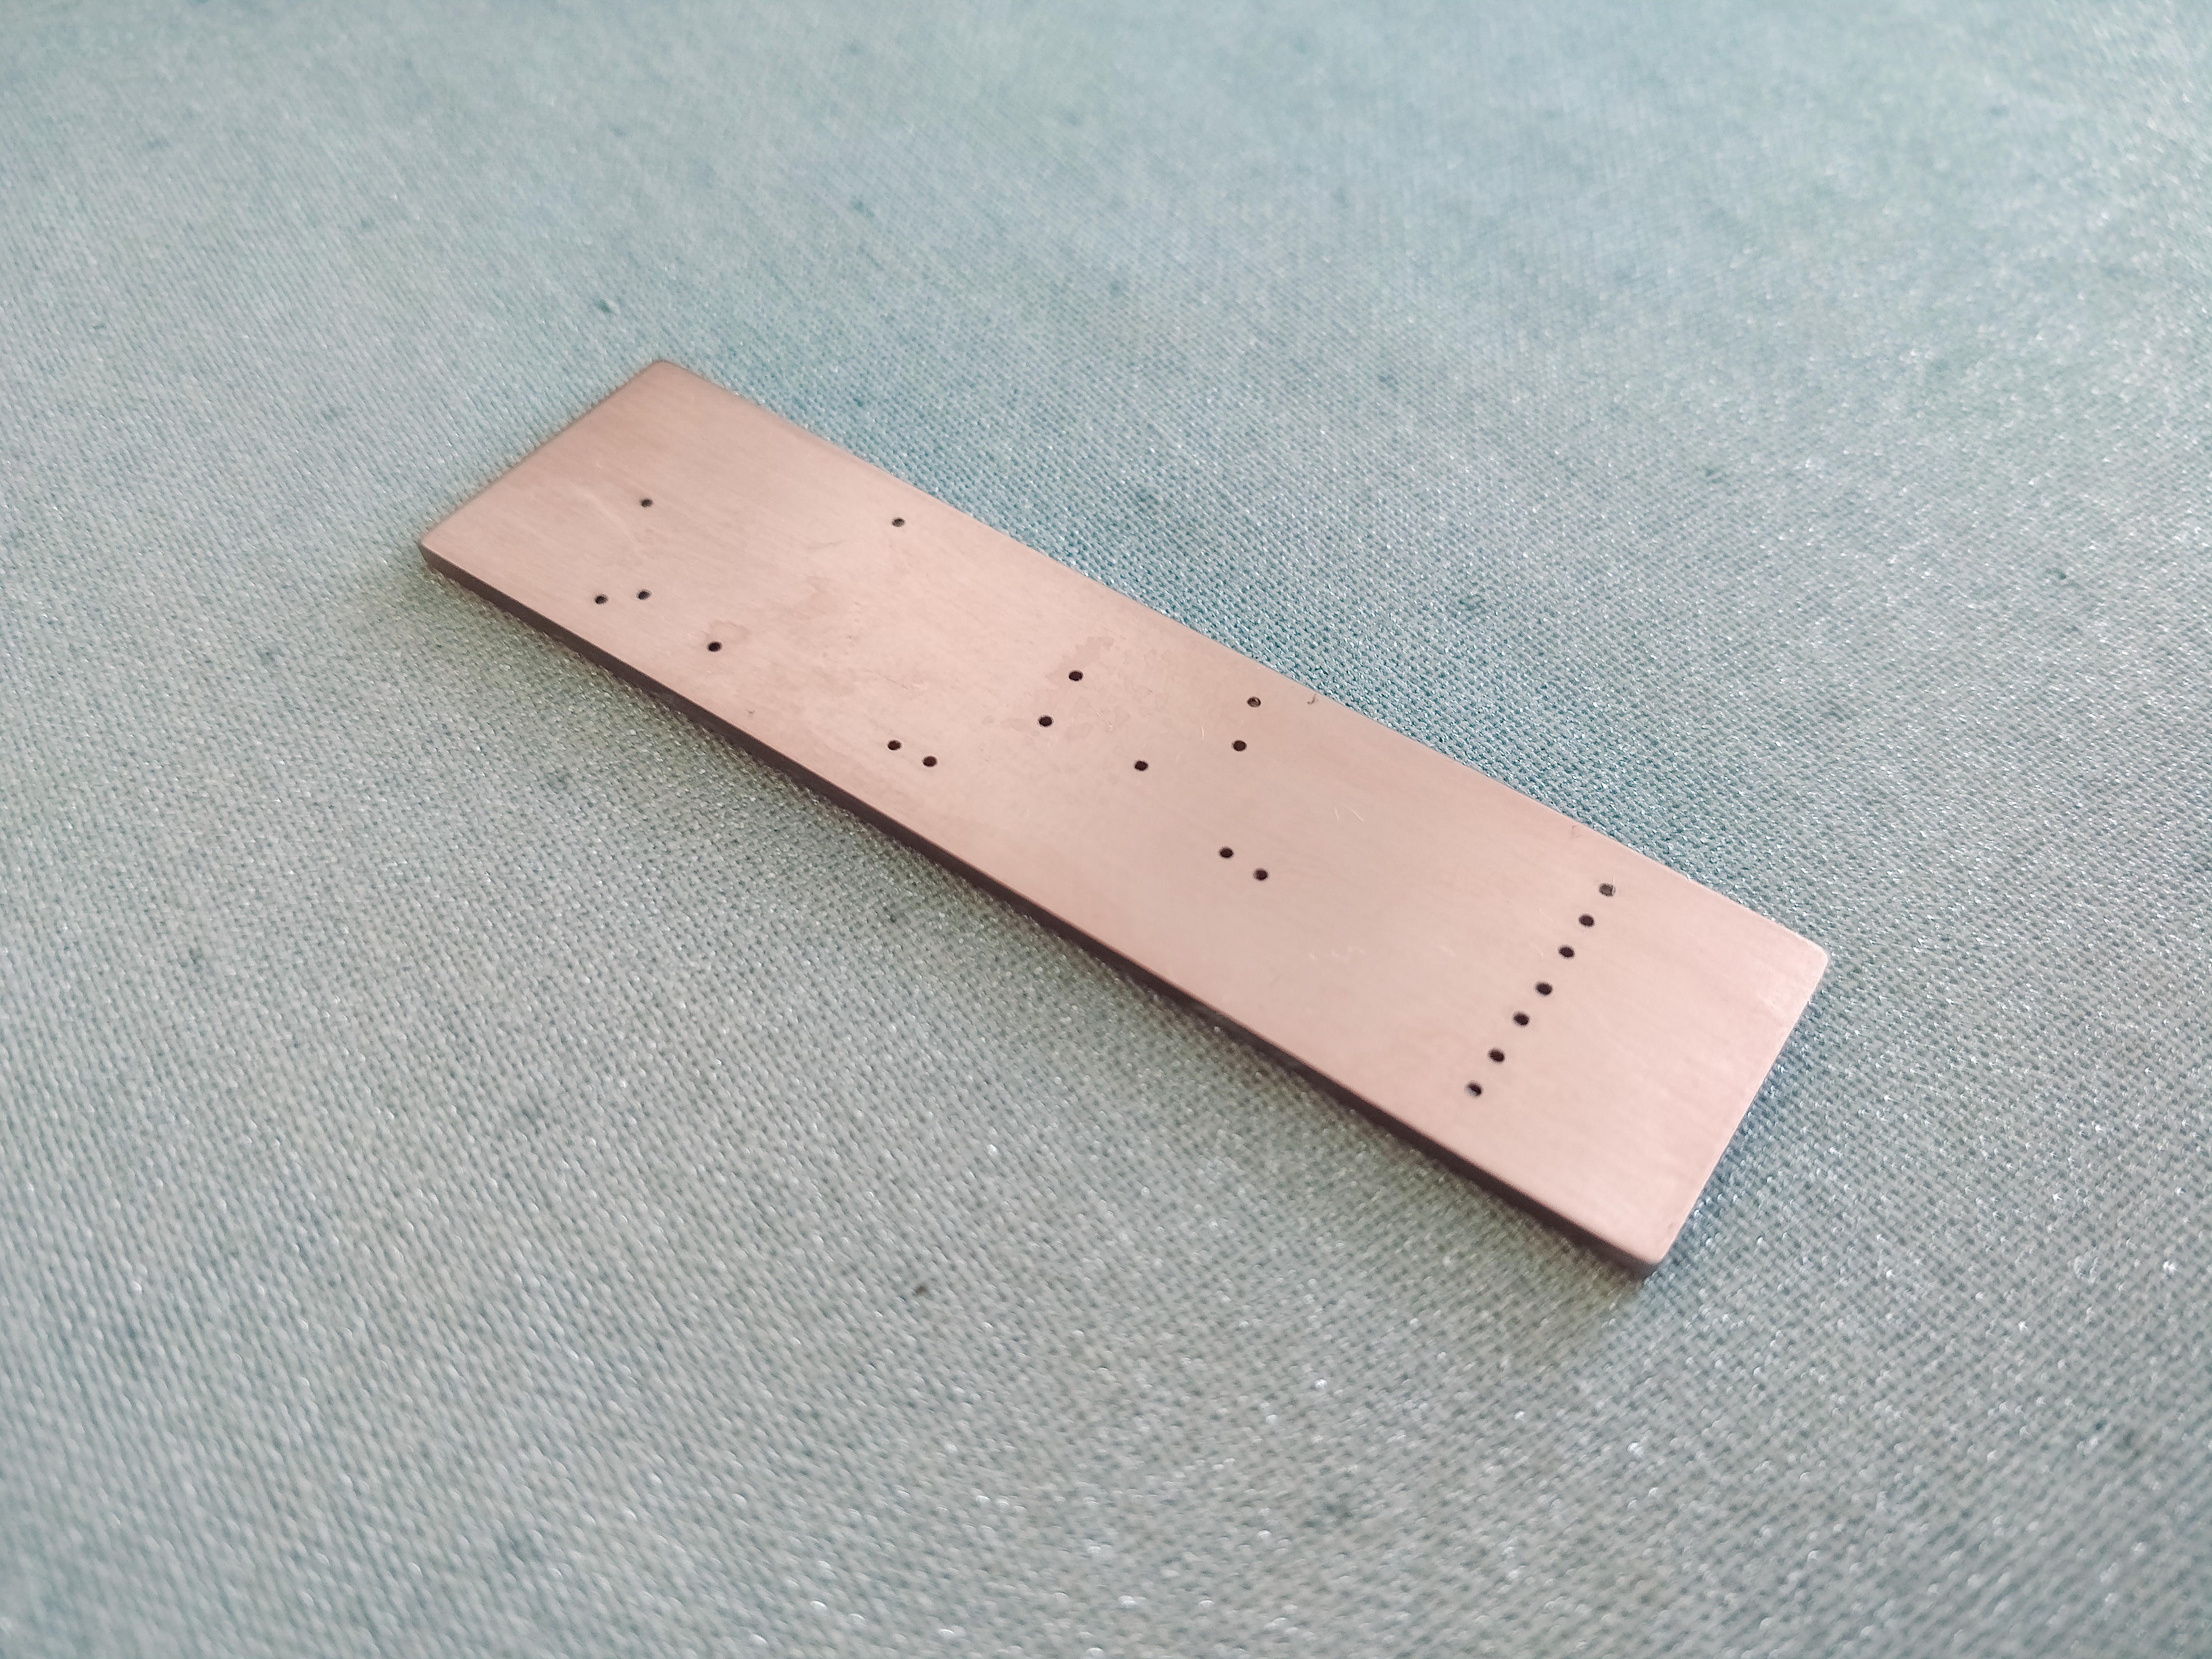
\includegraphics[width=\linewidth]{media/album/PSX_20220228_174045.jpg}
            \caption{}
            \label{fig:PhotoPCBDrill}
        \end{minipage}
    \end{figure}
    \clearpage

    Приготовив раствор\footnote{Рисунки \ref{fig:PhotoSolutionPrep}, \ref{fig:PhotoSolution}} FeCl3\footnote{Растворяемое вещество нужно добавлять в раствор понемногу, следя, чтобы температура не превышала $55^{\circ}C$ \parenciteit{p2}{FECL3:Datasheet}, поскольку процесс экзотермический} концентрацией 40\%\emph{(m/m)}\footnote{Я решил воспроизвести коммерческий раствор для травления плат \parenciteit{p1}{FECL3:Datasheet}}, я начал травление в хорошо проветриваемом месте\footnote{При реакции с медью может образовываться газ $Cl_2$: $FeCl_3 + Cu \Rightarrow CuCl + FeCl_2$ и затем $FeCl_2 + Cu \Rightarrow CuFe + Cl_2$}.

    \begin{figure}[H]
        \centering
        \begin{minipage}[H]{.525\linewidth}
            \centering
            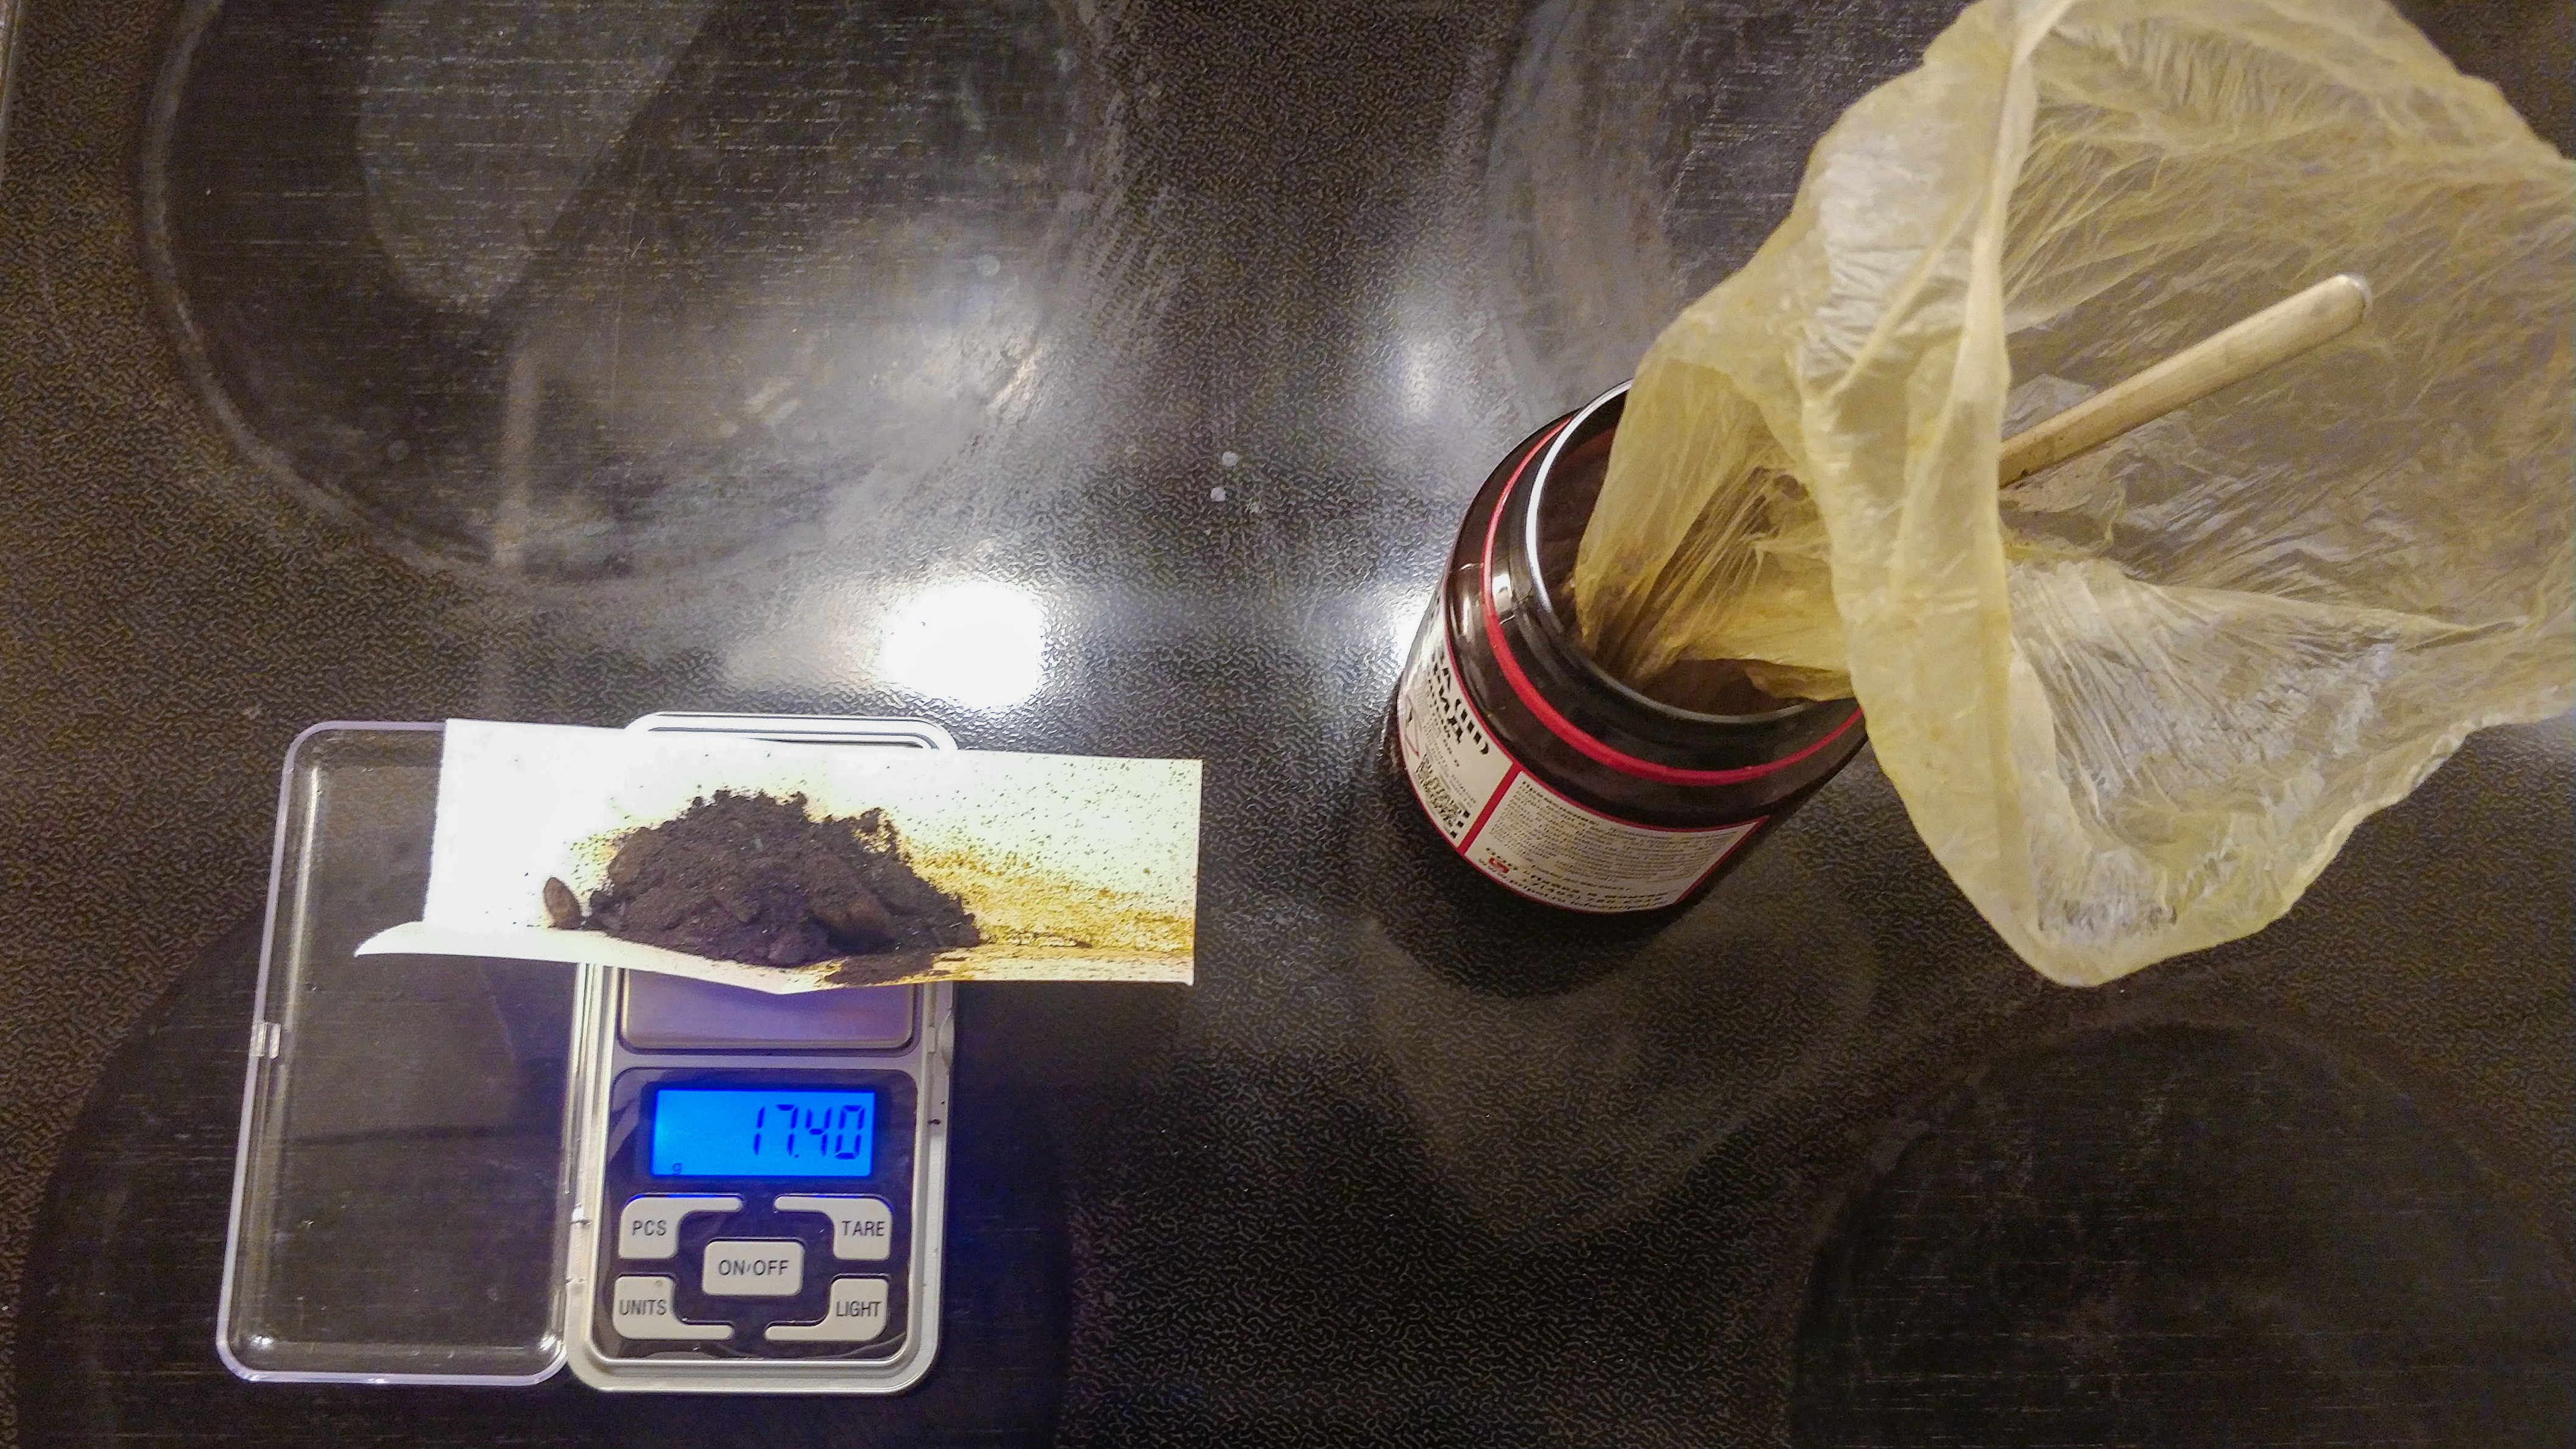
\includegraphics[width=\linewidth]{media/album/PSX_20220228_160724.jpg}
            \caption{}
            \label{fig:PhotoSolutionPrep}
        \end{minipage}
        \hspace{.04\linewidth}
        \begin{minipage}[H]{.394\linewidth}
            \centering
            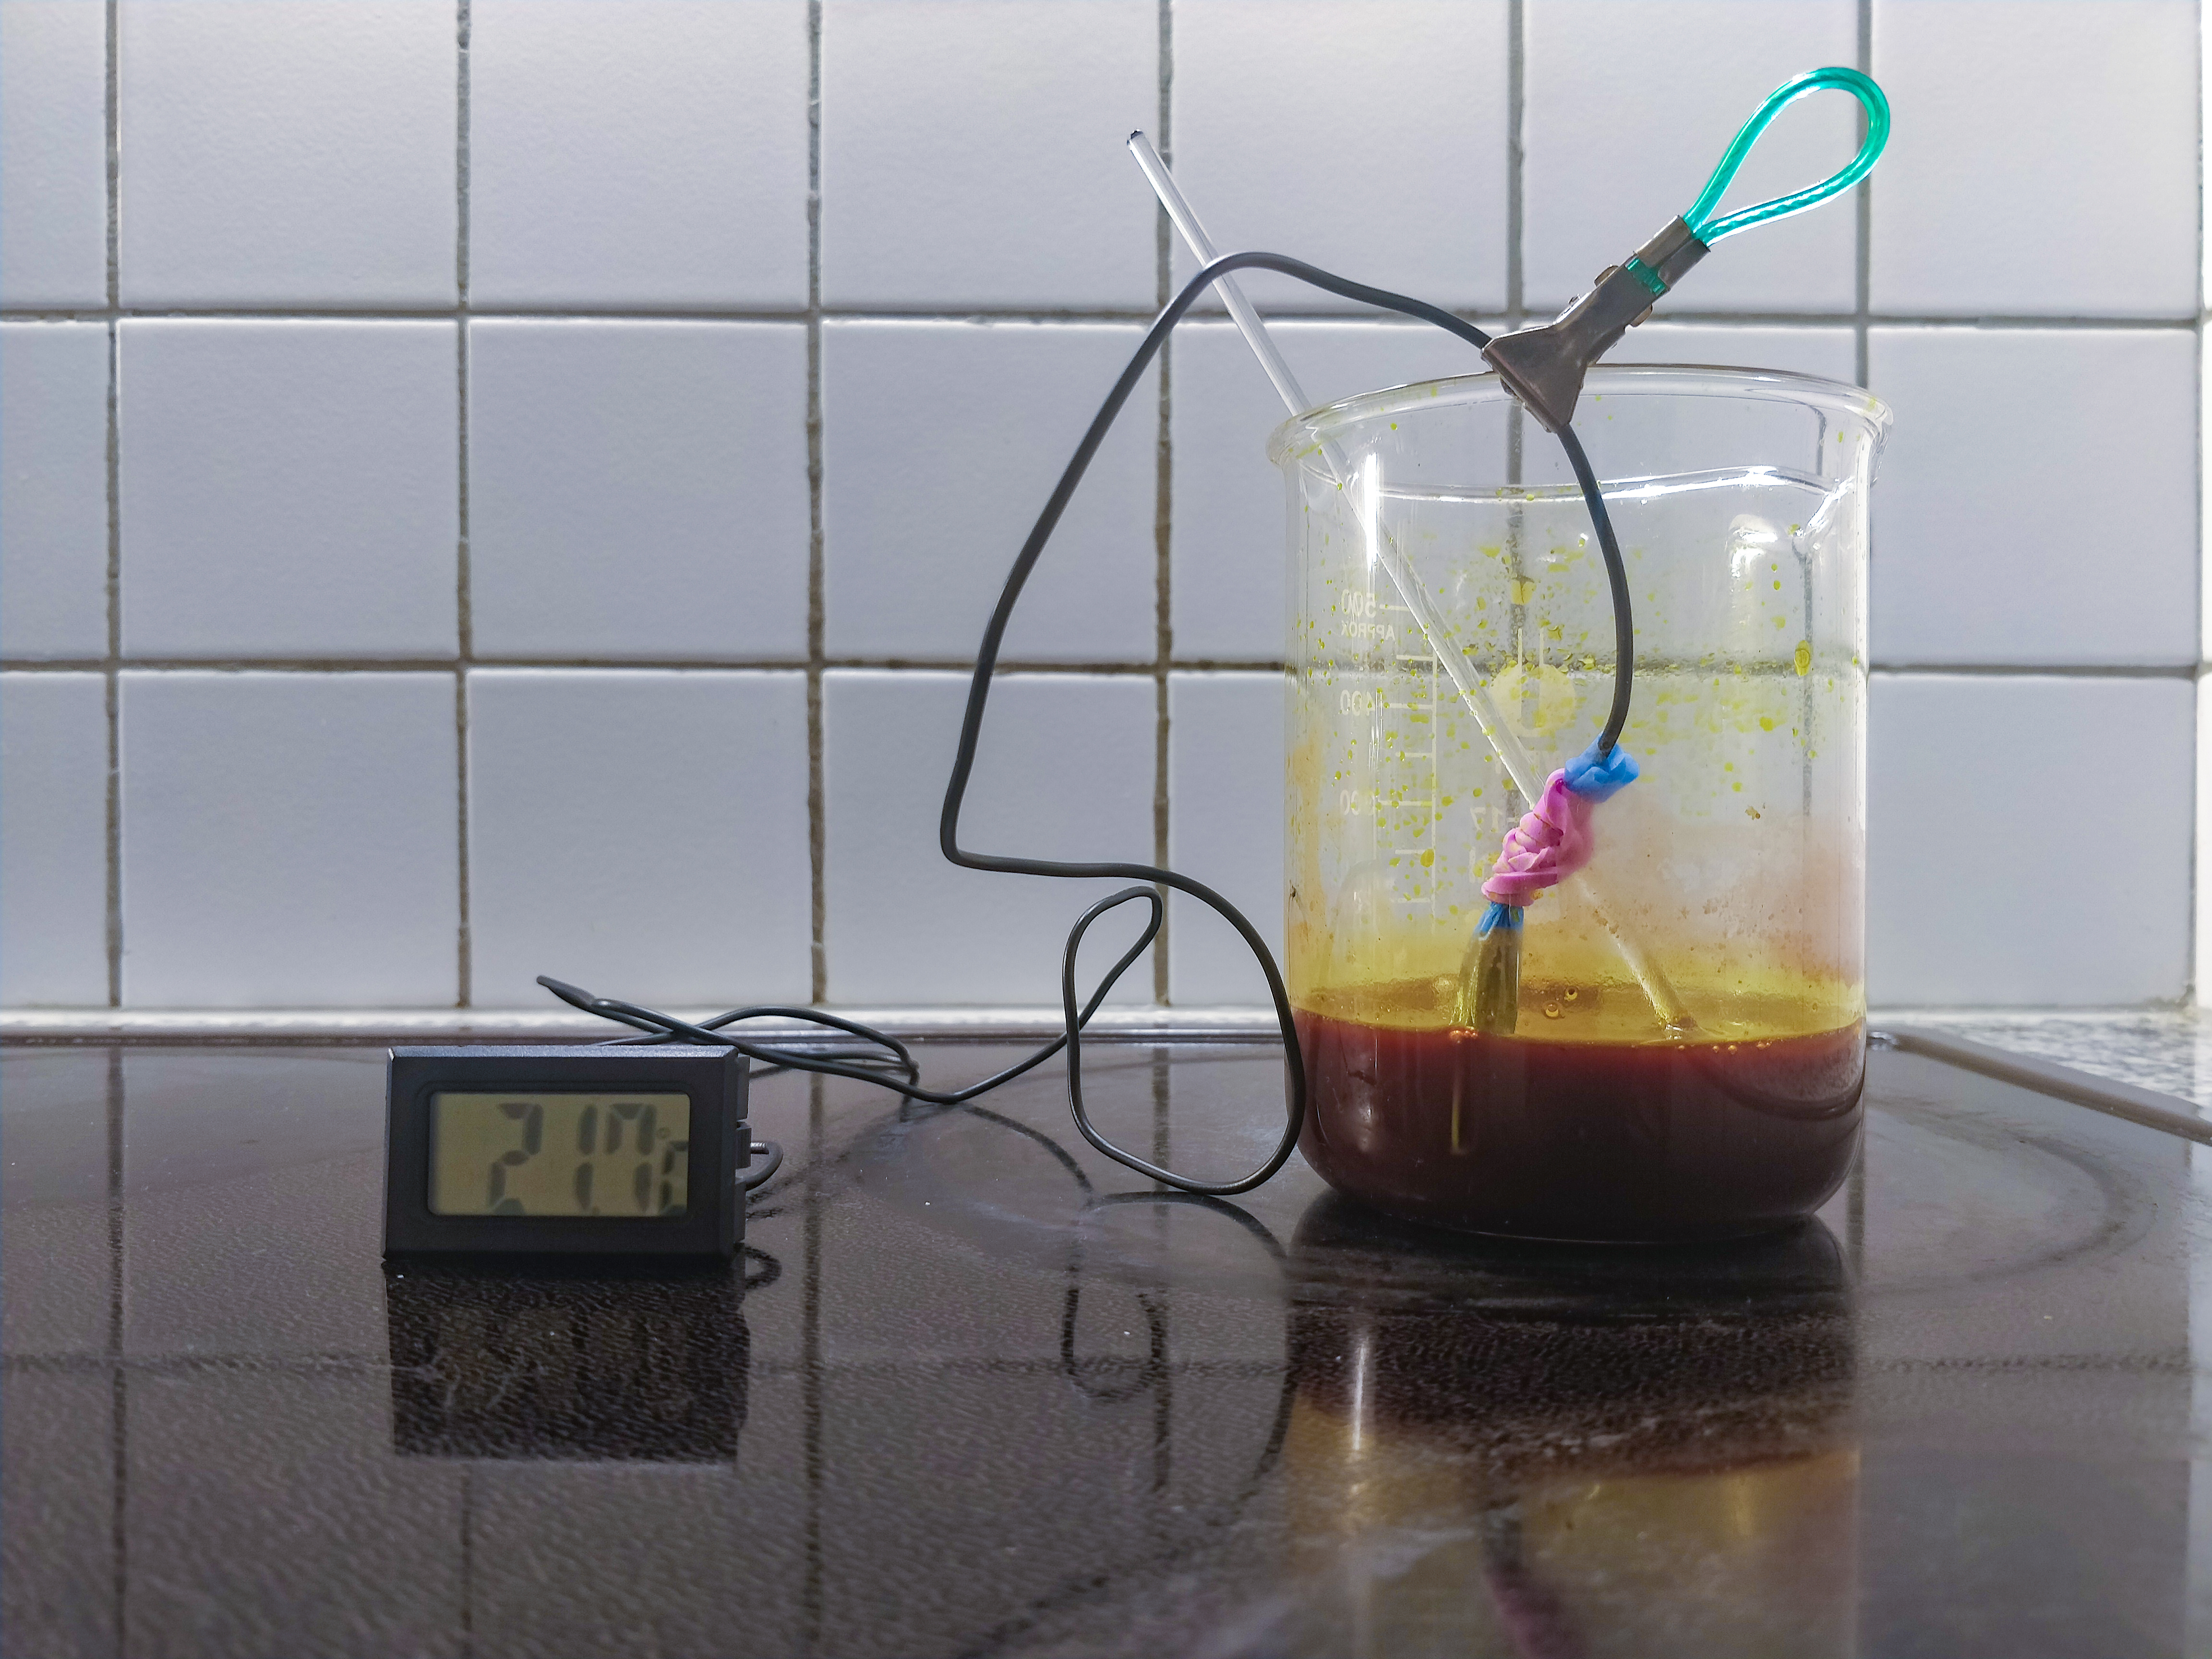
\includegraphics[width=\linewidth]{media/album/PSX_20220301_014813.jpg}
            \caption{}
            \label{fig:PhotoSolution}
        \end{minipage}
    \end{figure}


    Процесс следует технологии, общей для всех самодельных (DIY\footnote{Do-It-Yourself, «сделай сам»}) плат: как уже говорилось, нужно распечатать схему на листе бумаги, положить его отпечатанной стороной на чистую поверхность подготовленной заготовки и перенести тонер кратковременным нагревом\footnote{Обычно используют утюг}\:\footnote{Рисунок \ref{fig:PhotoPCBIron}}.
    Затем лист со схемой нужно осторожно снять\footnote{Рисунок\ref{fig:PhotoPCBWash}}.
    Самый эффективный способ --- намочить бумагу и понемногу стирать её чем-нибудь шероховатым, но мягким, например губкой.
    Полностью очистив схему, я получил дорожки тонера, прикипевшие к поверхности платы.
    Они будут защищать от травящего раствора: открытые участки будут реагировать с раствором и со временем растворяться, а закрытые останутся на месте.

    \begin{figure}[H]
        \centering
        \begin{minipage}[H]{.331\linewidth}
            \centering
            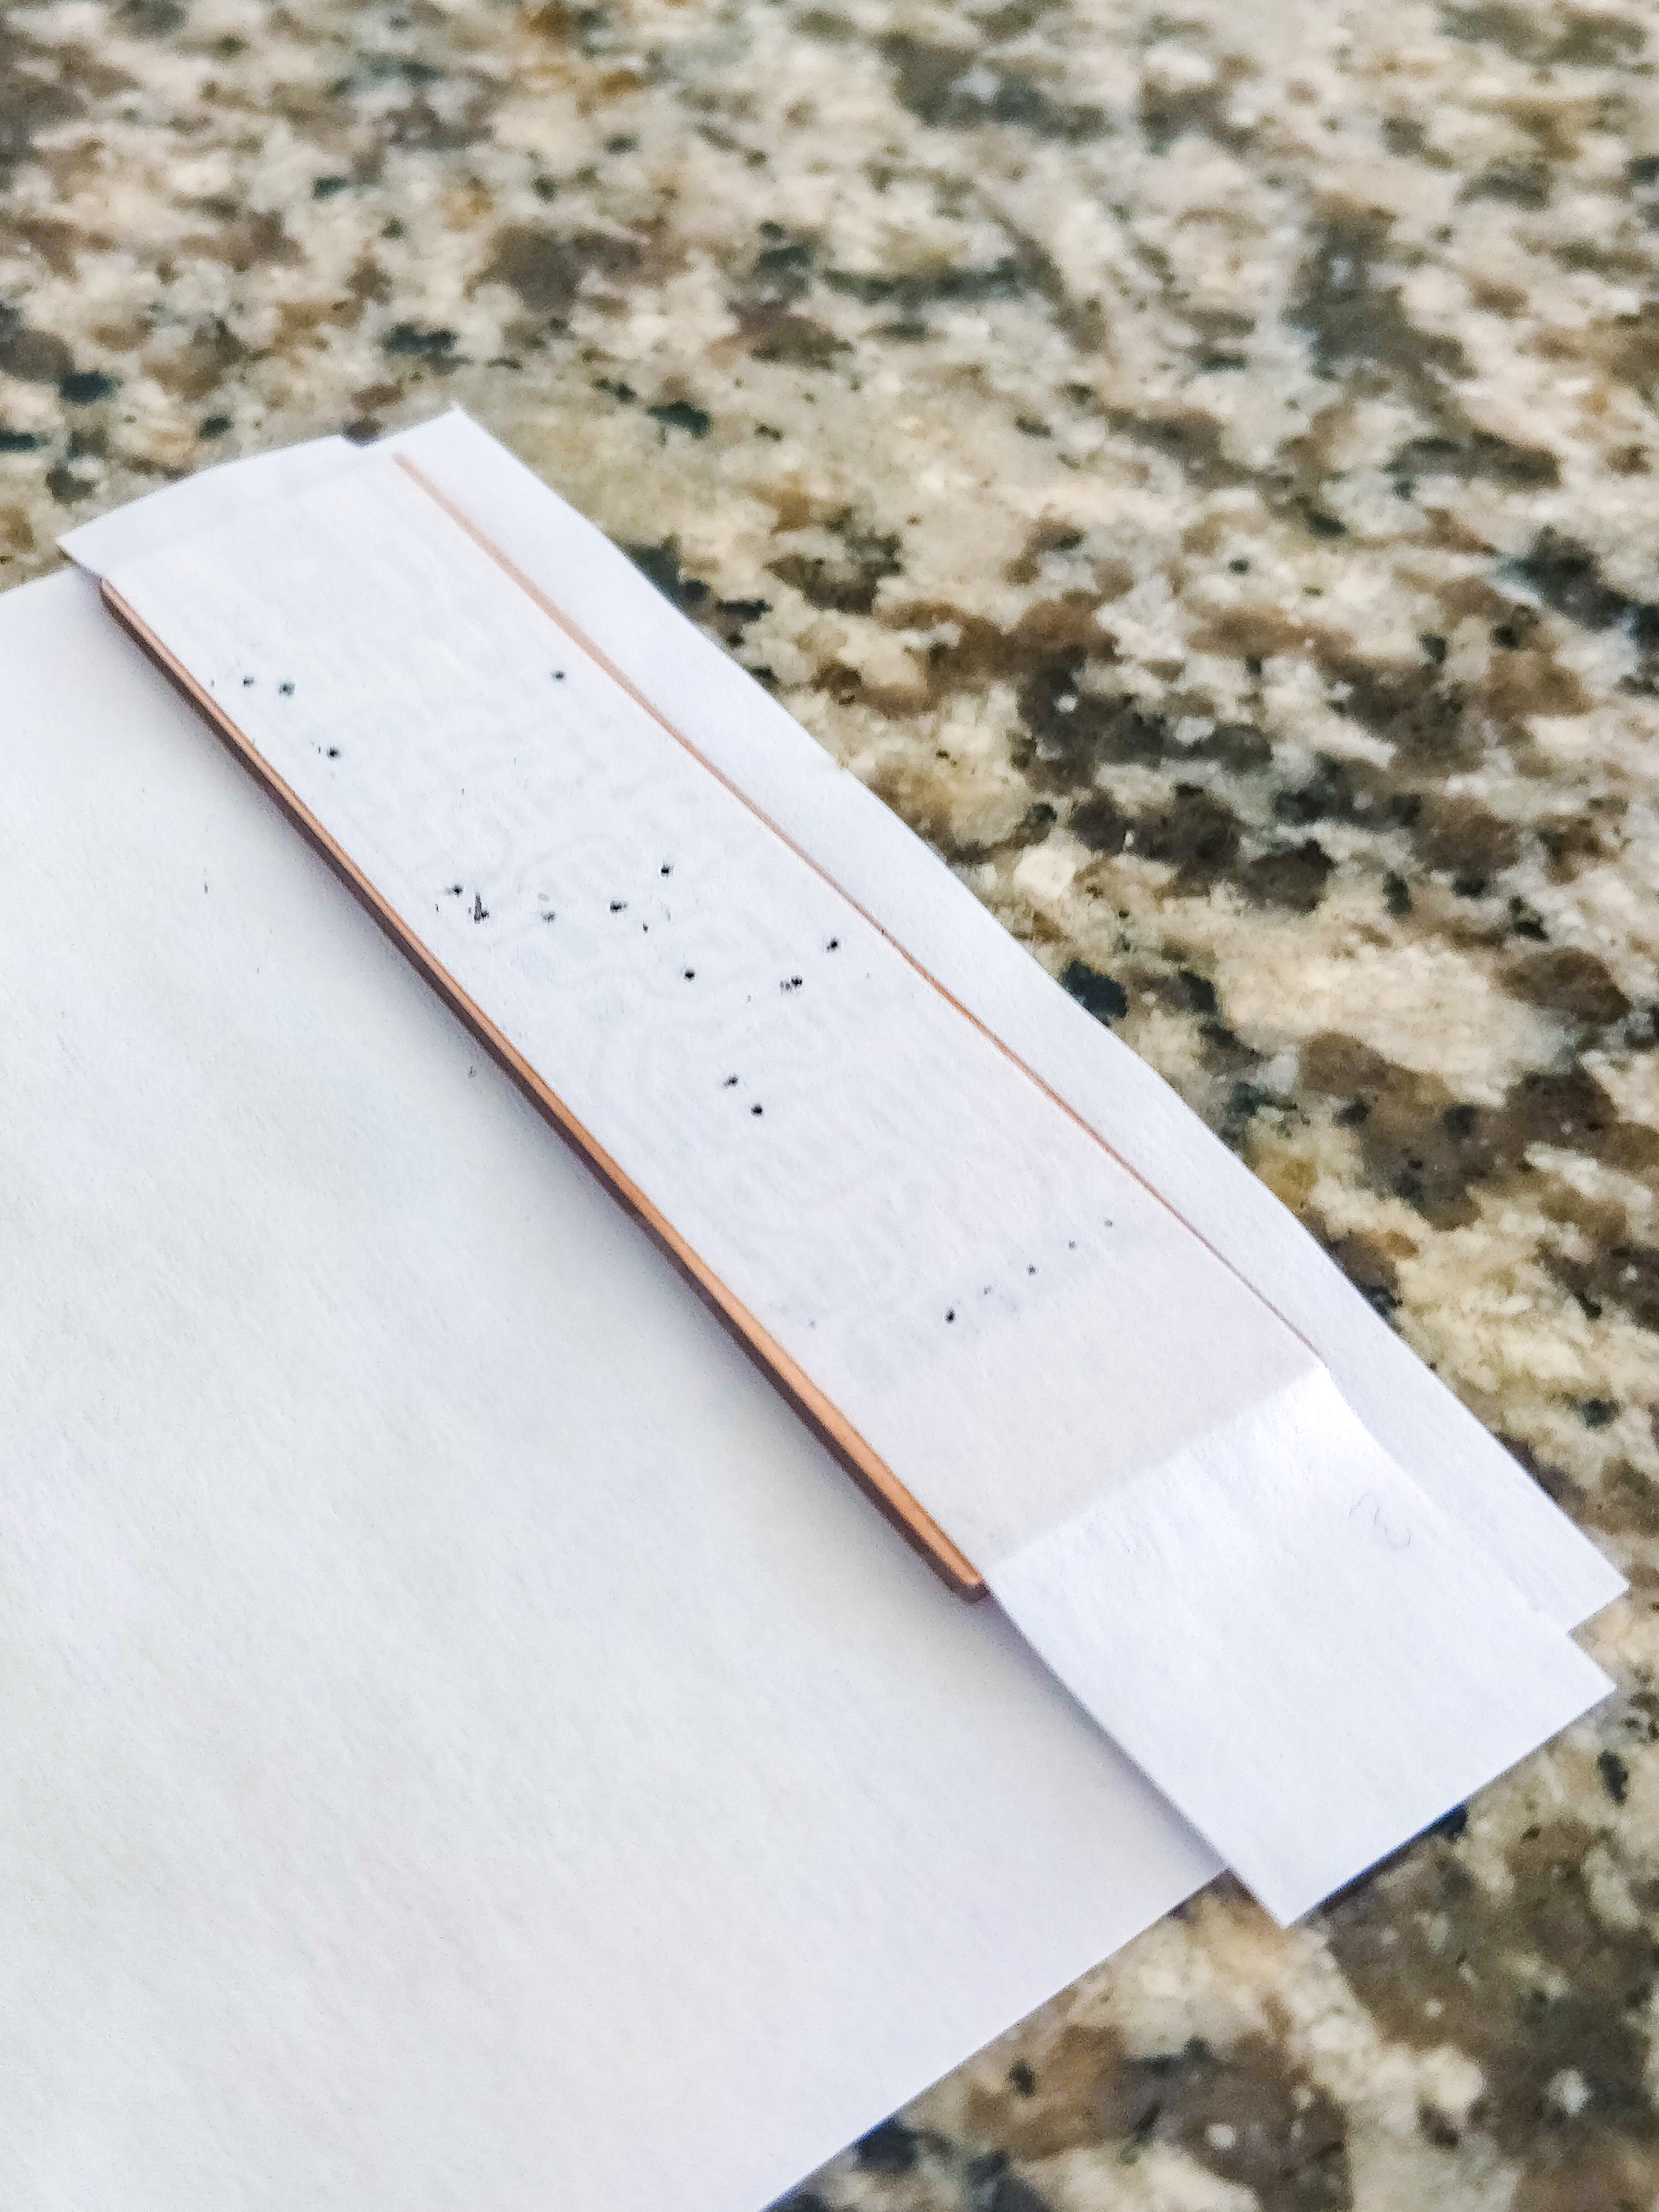
\includegraphics[width=\linewidth]{media/album/PSX_20220228_020336.jpg}
            \caption{}
            \label{fig:PhotoPCBIron}
        \end{minipage}
        \hspace{.04\linewidth}
        \begin{minipage}[H]{.5888\linewidth}
            \centering
            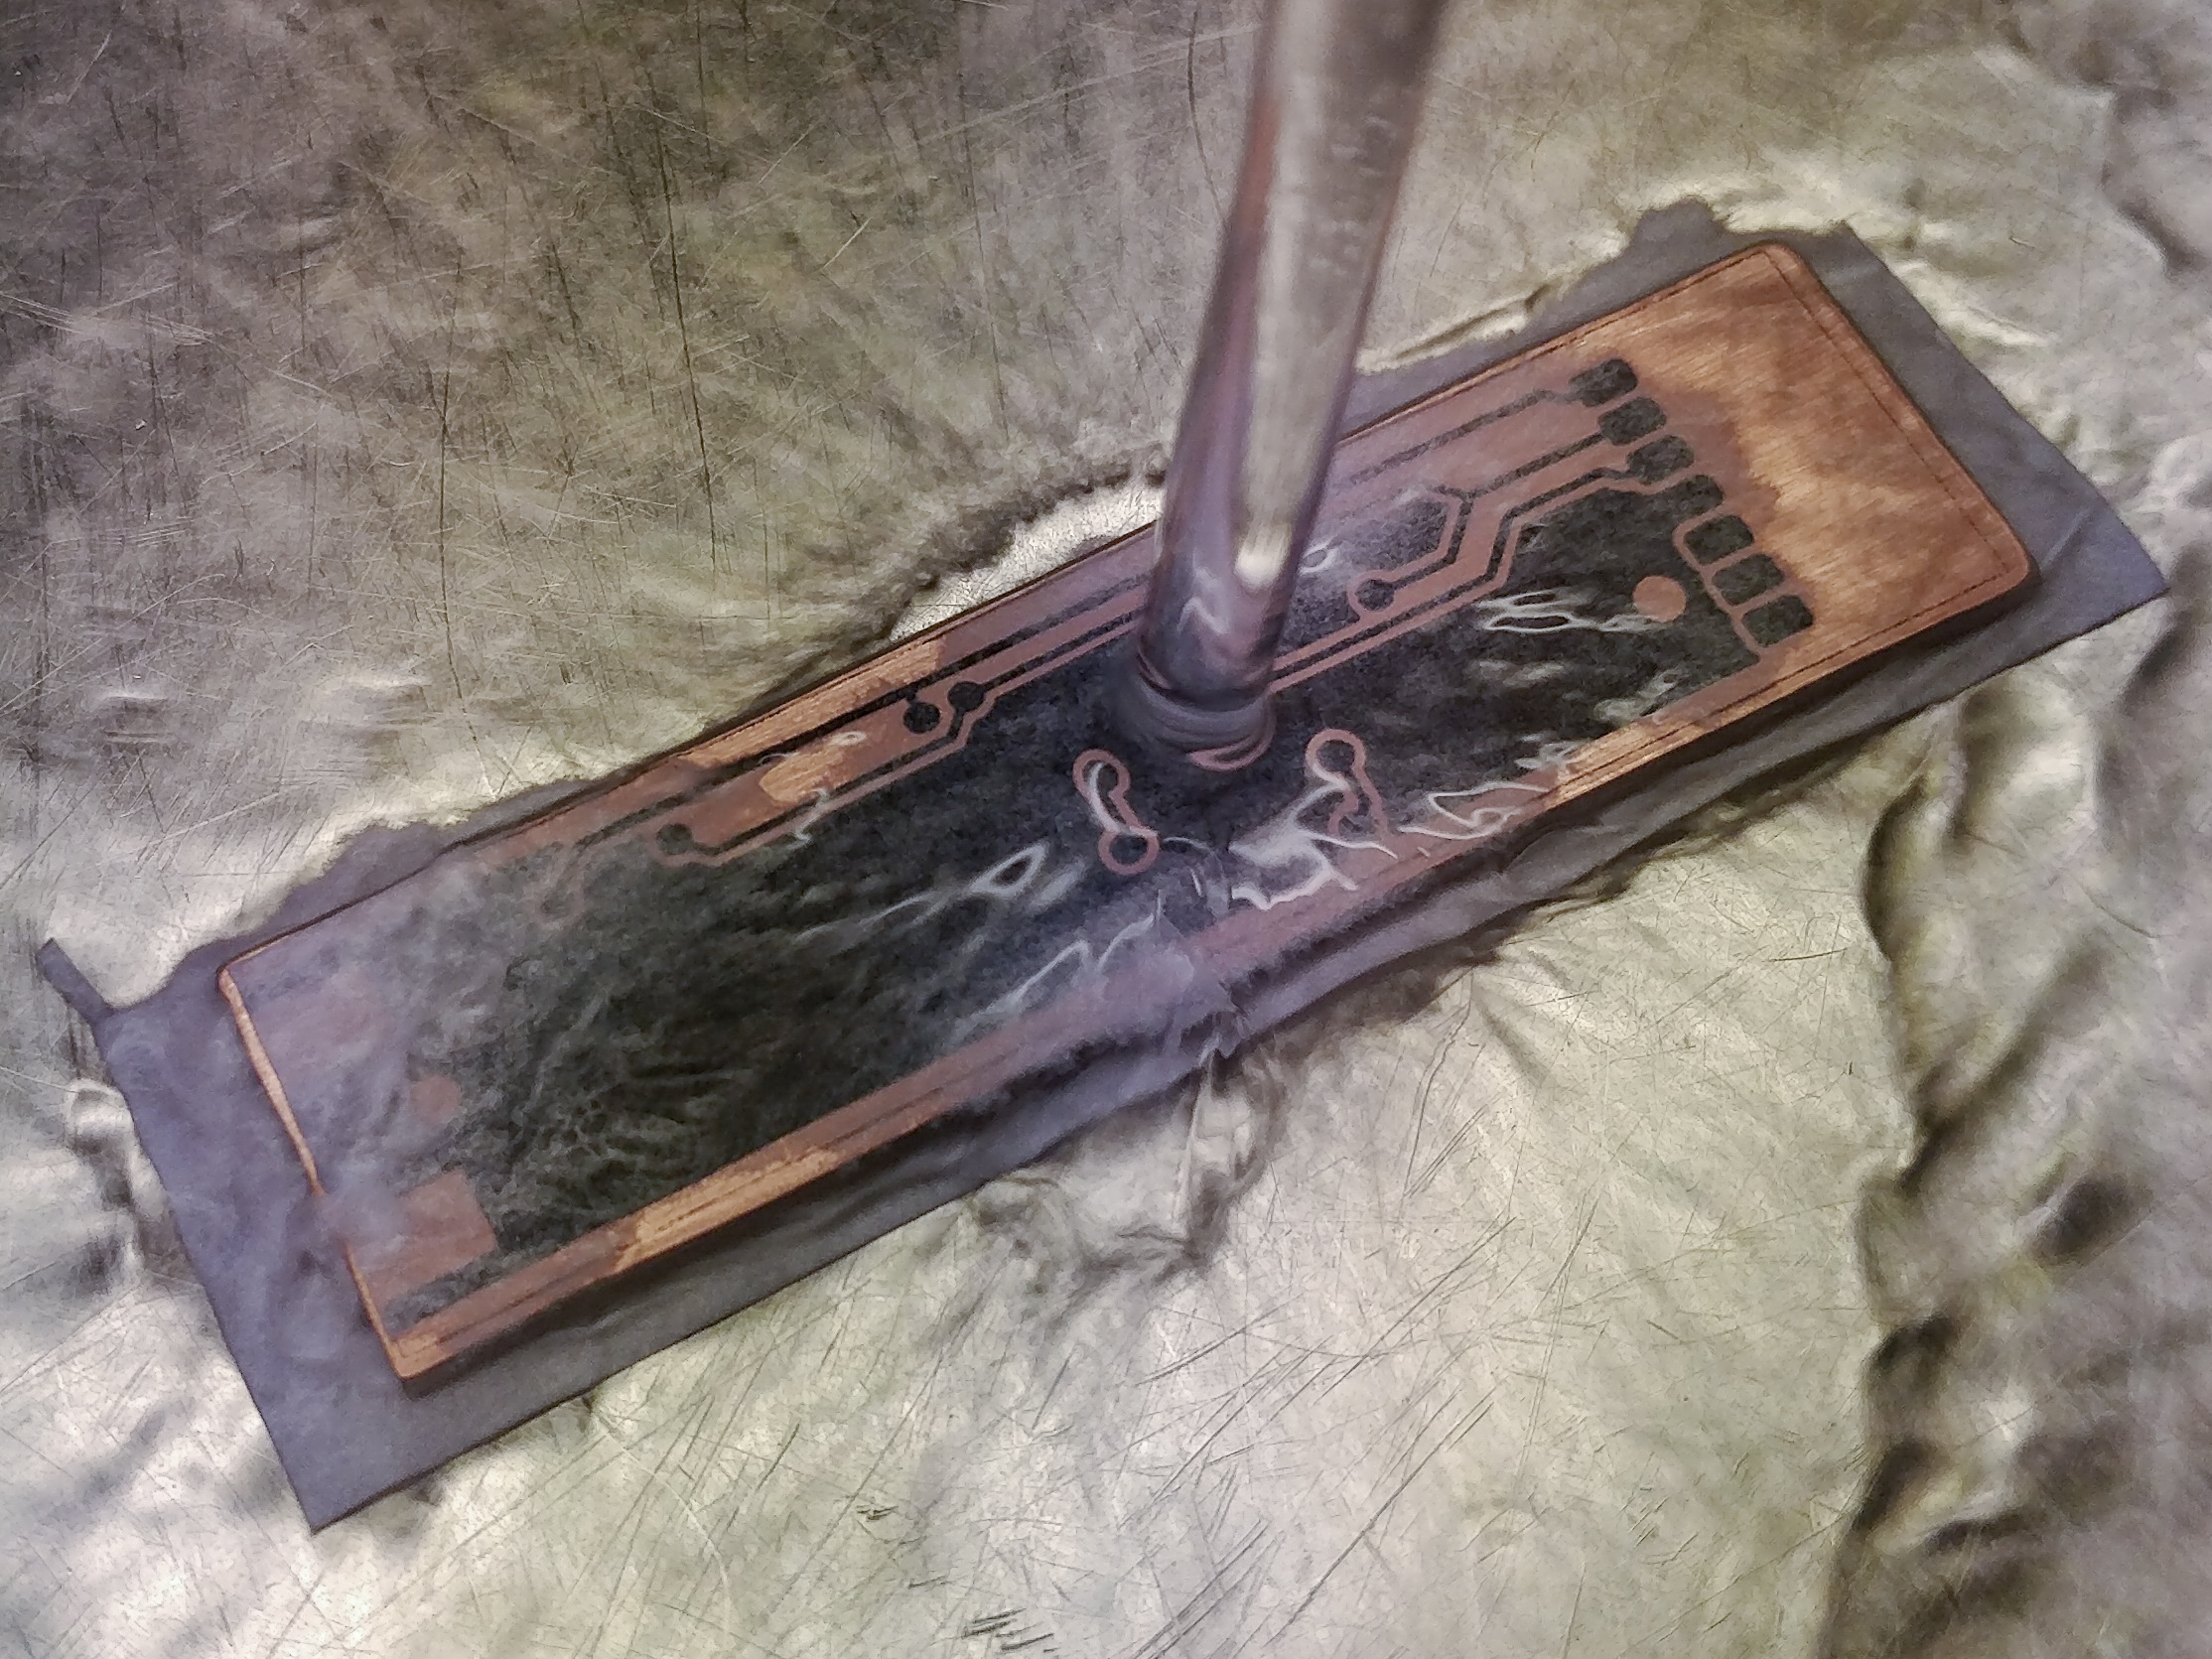
\includegraphics[width=\linewidth]{media/album/PSX_20220301_034705.jpg}
            \caption{}
            \label{fig:PhotoPCBWash}
        \end{minipage}
    \end{figure}
    \clearpage

    Около 10 минут схема находилась\footnote{Рисунки \ref{fig:PhotoPCBPrepare1}, \ref{fig:PhotoPCBPrepare2}, \ref{fig:PhotoPCBPrepare3}, \ref{fig:PhotoPCBPrepareDone}} в растворе, пока медь понемногу растворялась.
    Кроме того, раствор можно немного подогреть, чтобы ускорить процесс \emph{(опять же не превышая $55^{\circ}C$)}
    \begin{figure}[H]
        \centering
        \begin{minipage}[H]{.45\linewidth}
            \centering
            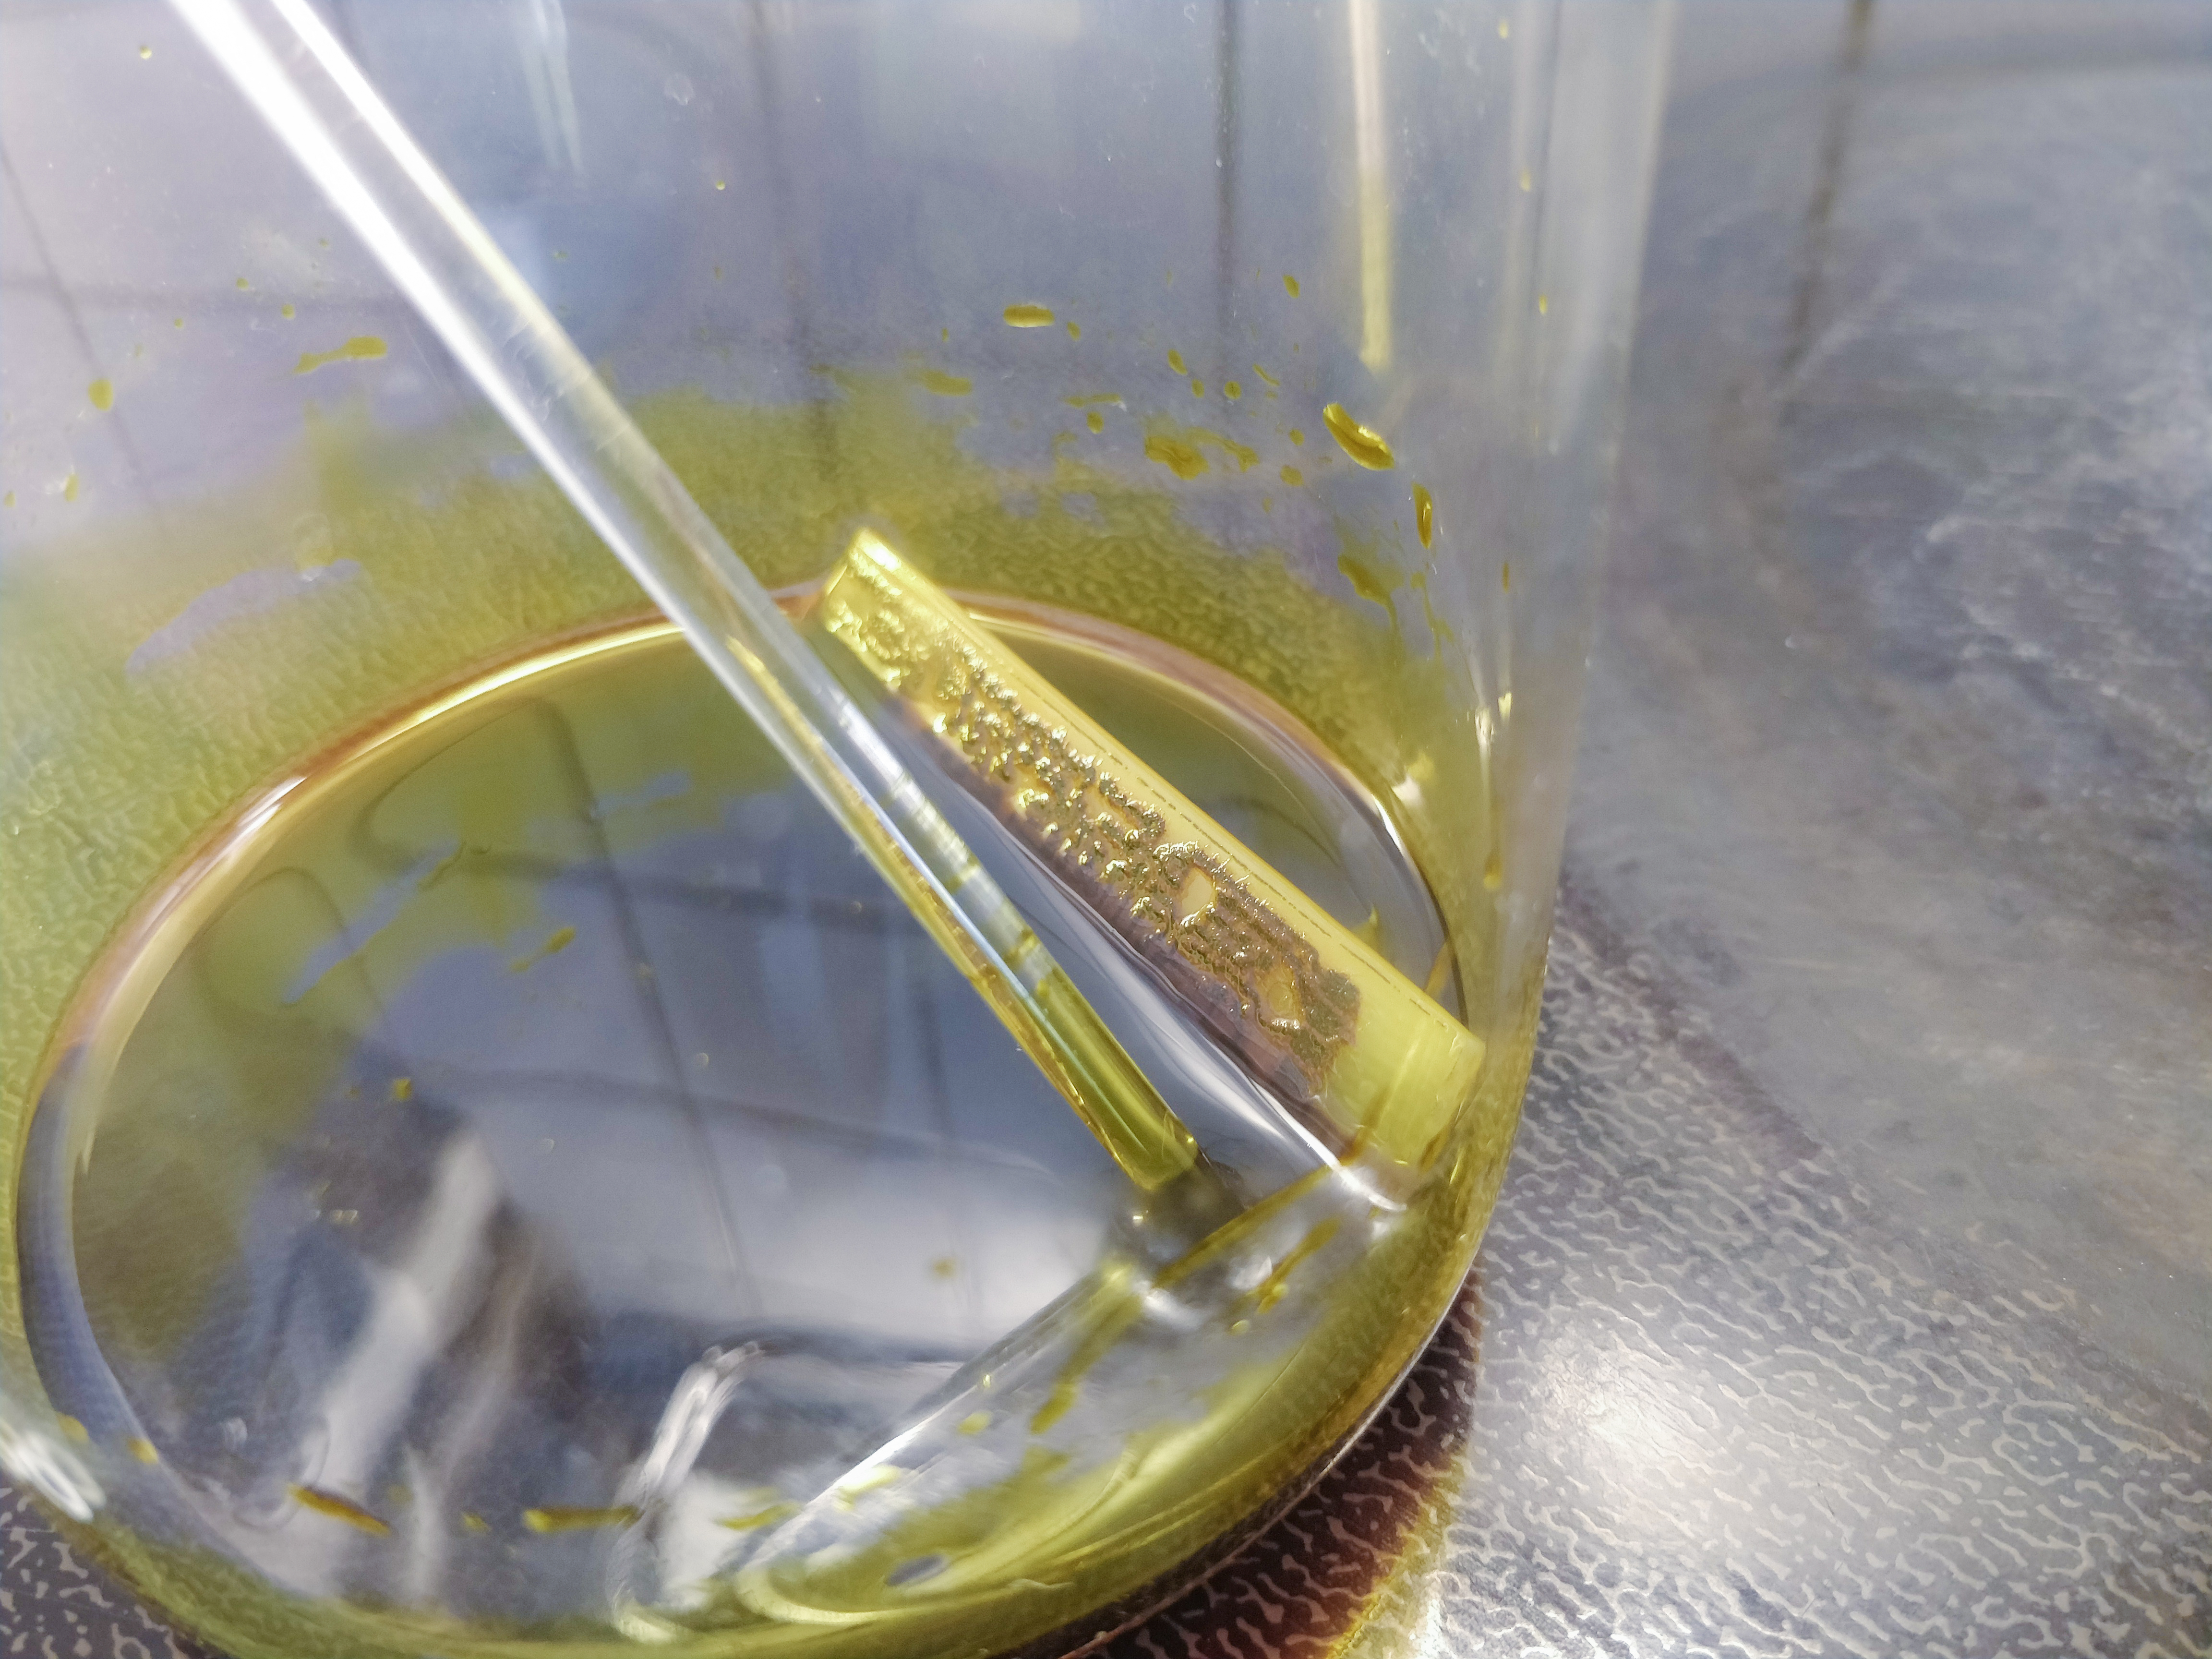
\includegraphics[width=\linewidth]{media/album/PSX_20220301_014718.jpg}
            \caption{}
            \label{fig:PhotoPCBPrepare1}
        \end{minipage}
        \hspace{.04\linewidth}
        \begin{minipage}[H]{.45\linewidth}
            \centering
            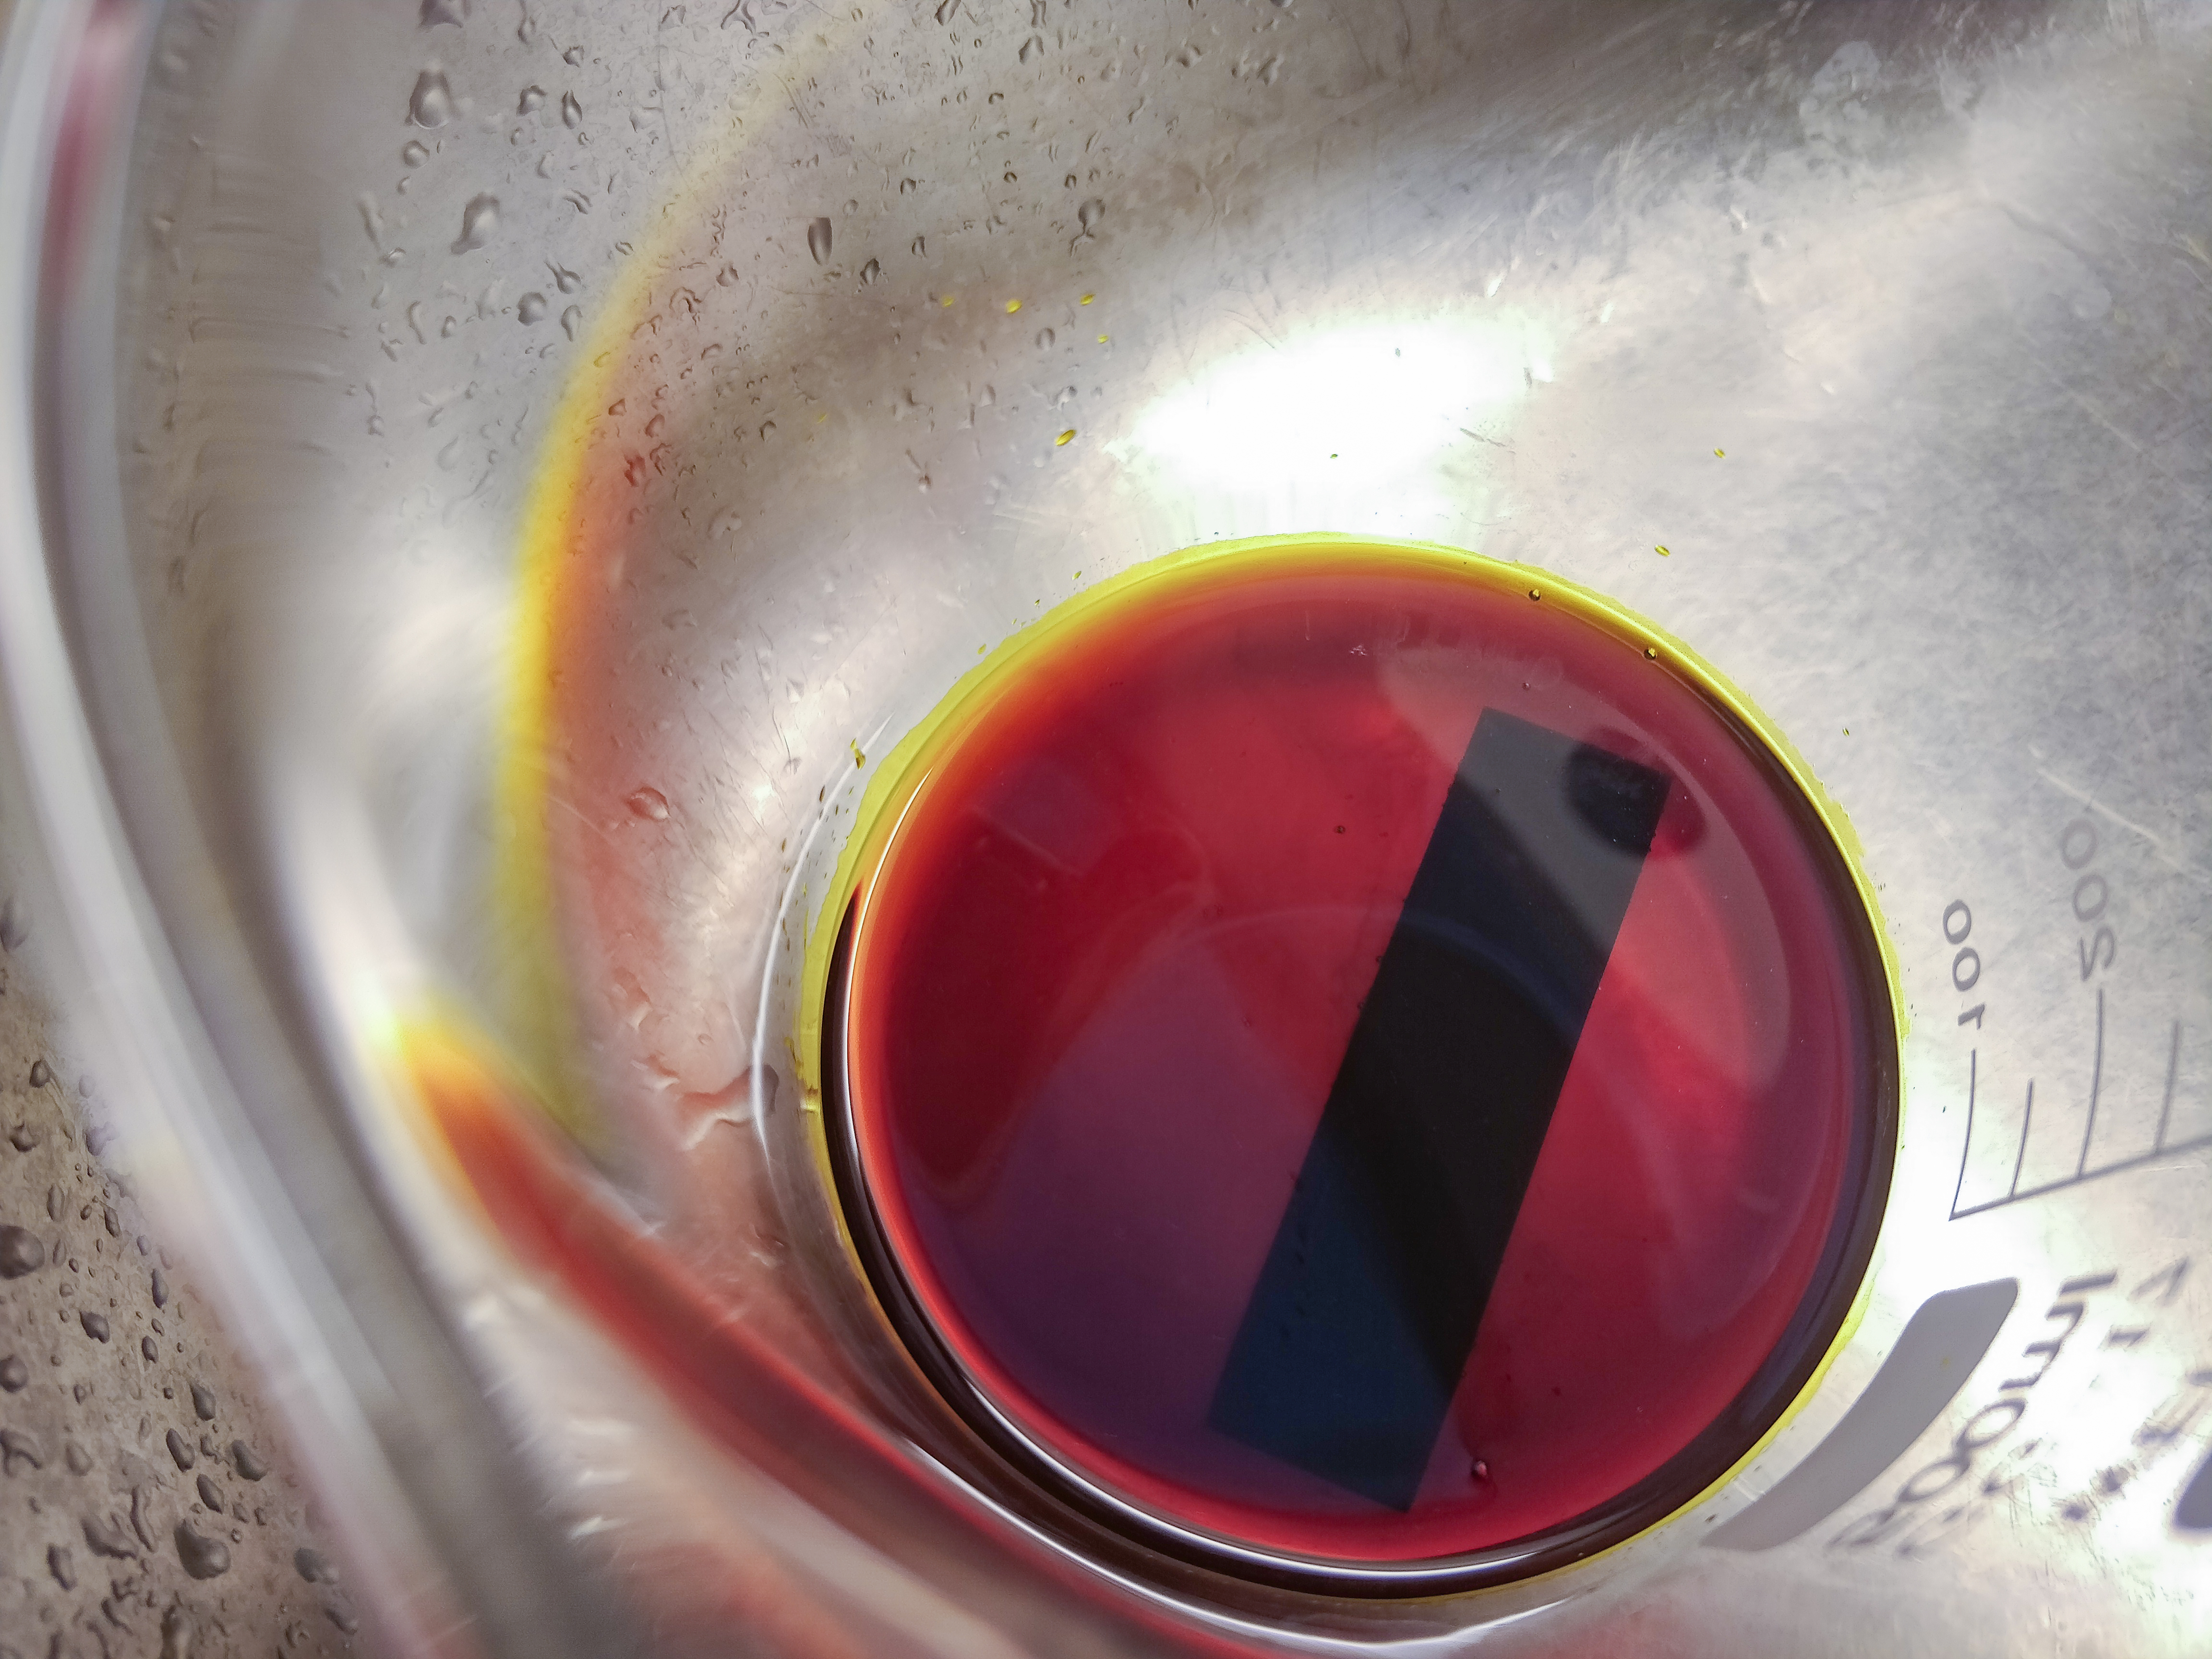
\includegraphics[width=\linewidth]{media/album/PSX_20220301_014557.jpg}
            \caption{}
            \label{fig:PhotoPCBPrepare2}
        \end{minipage}
        \\
        \vspace*{.01\linewidth}
        \begin{minipage}[H]{.95\linewidth}
            \centering
            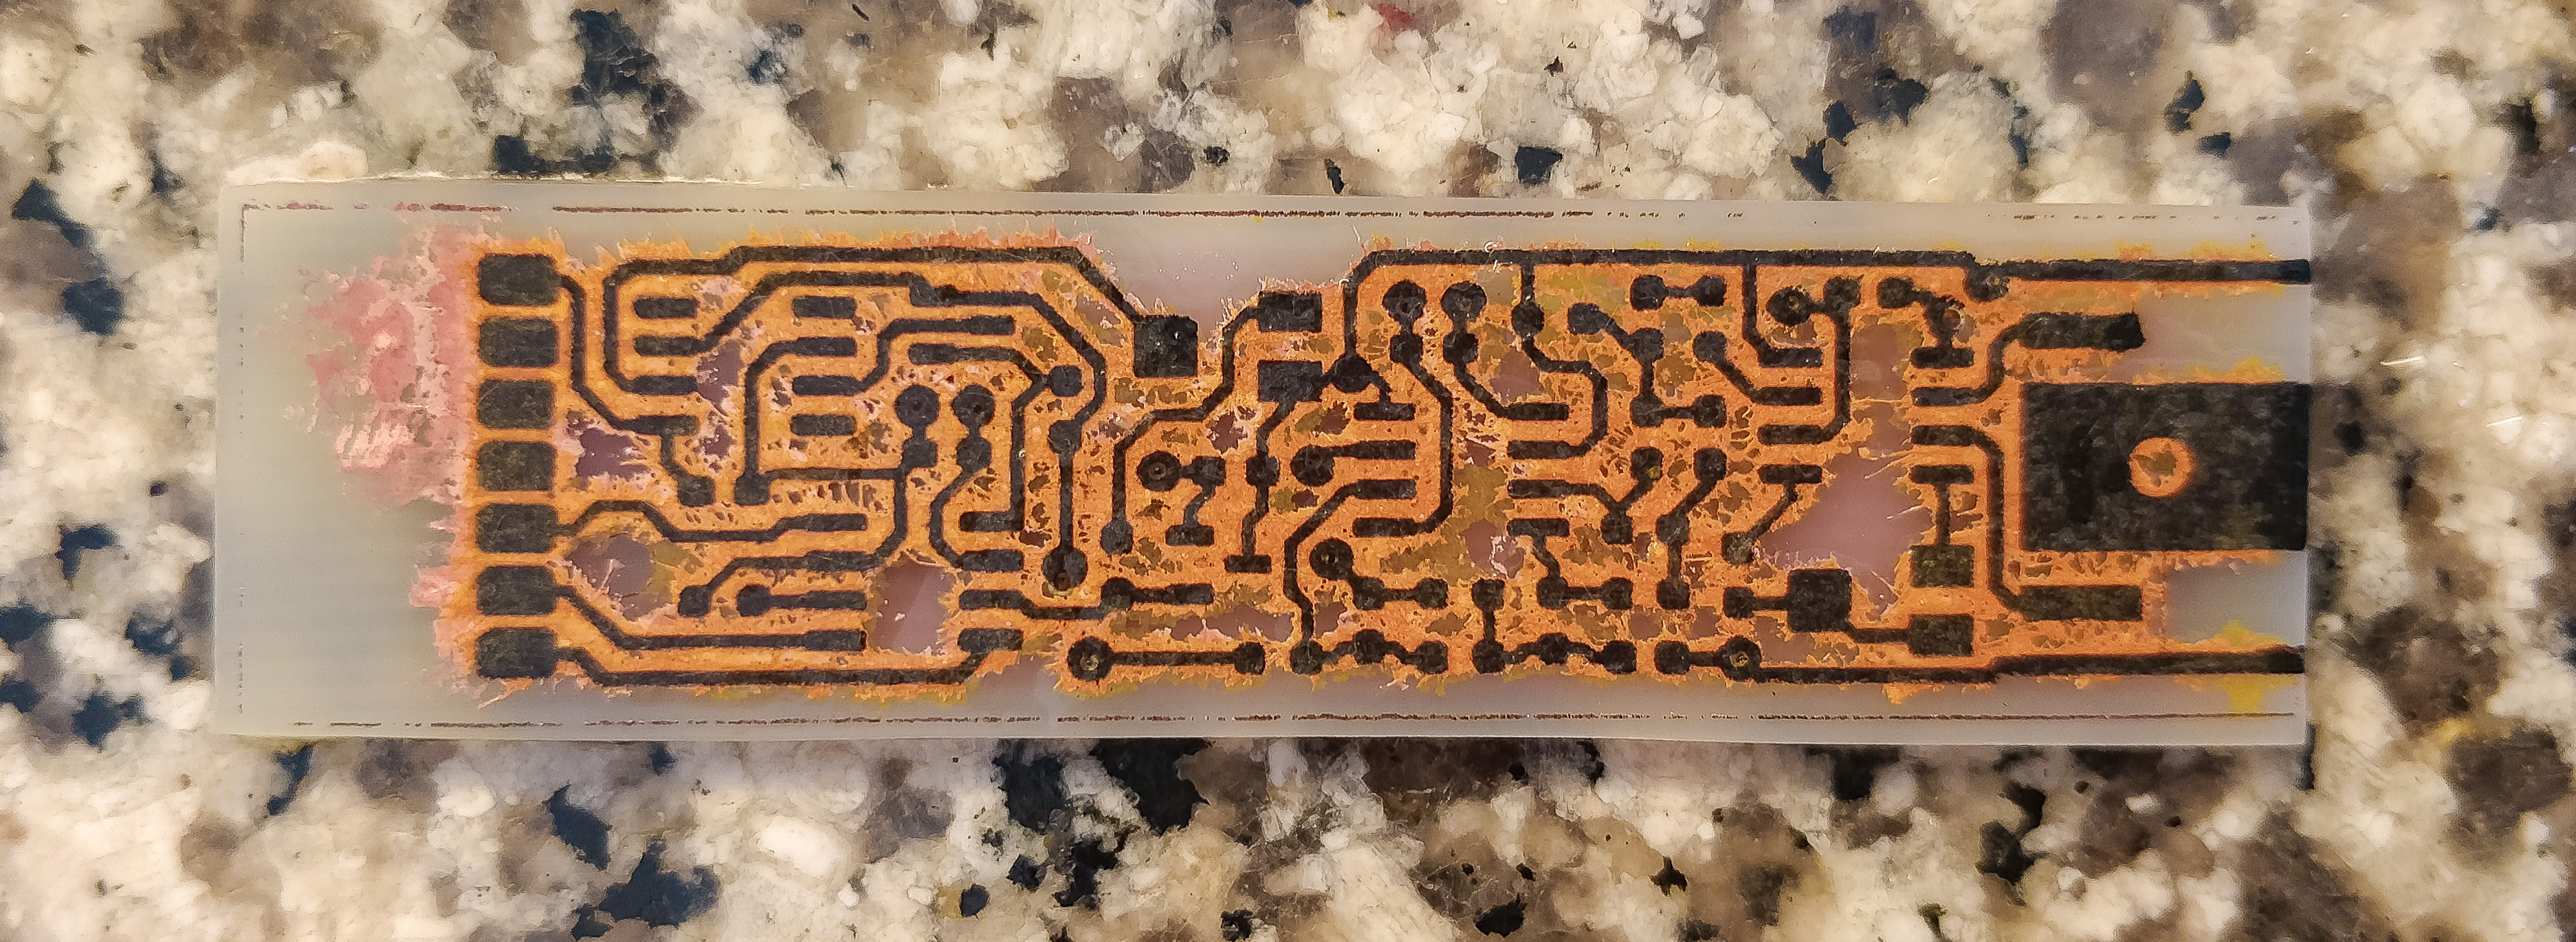
\includegraphics[width=\linewidth]{media/album/PSX_20220228_015716.jpg}
            \caption{}
            \label{fig:PhotoPCBPrepare3}
        \end{minipage}
        \\
        \vspace*{.01\linewidth}
        \begin{minipage}[H]{.95\linewidth}
            \centering
            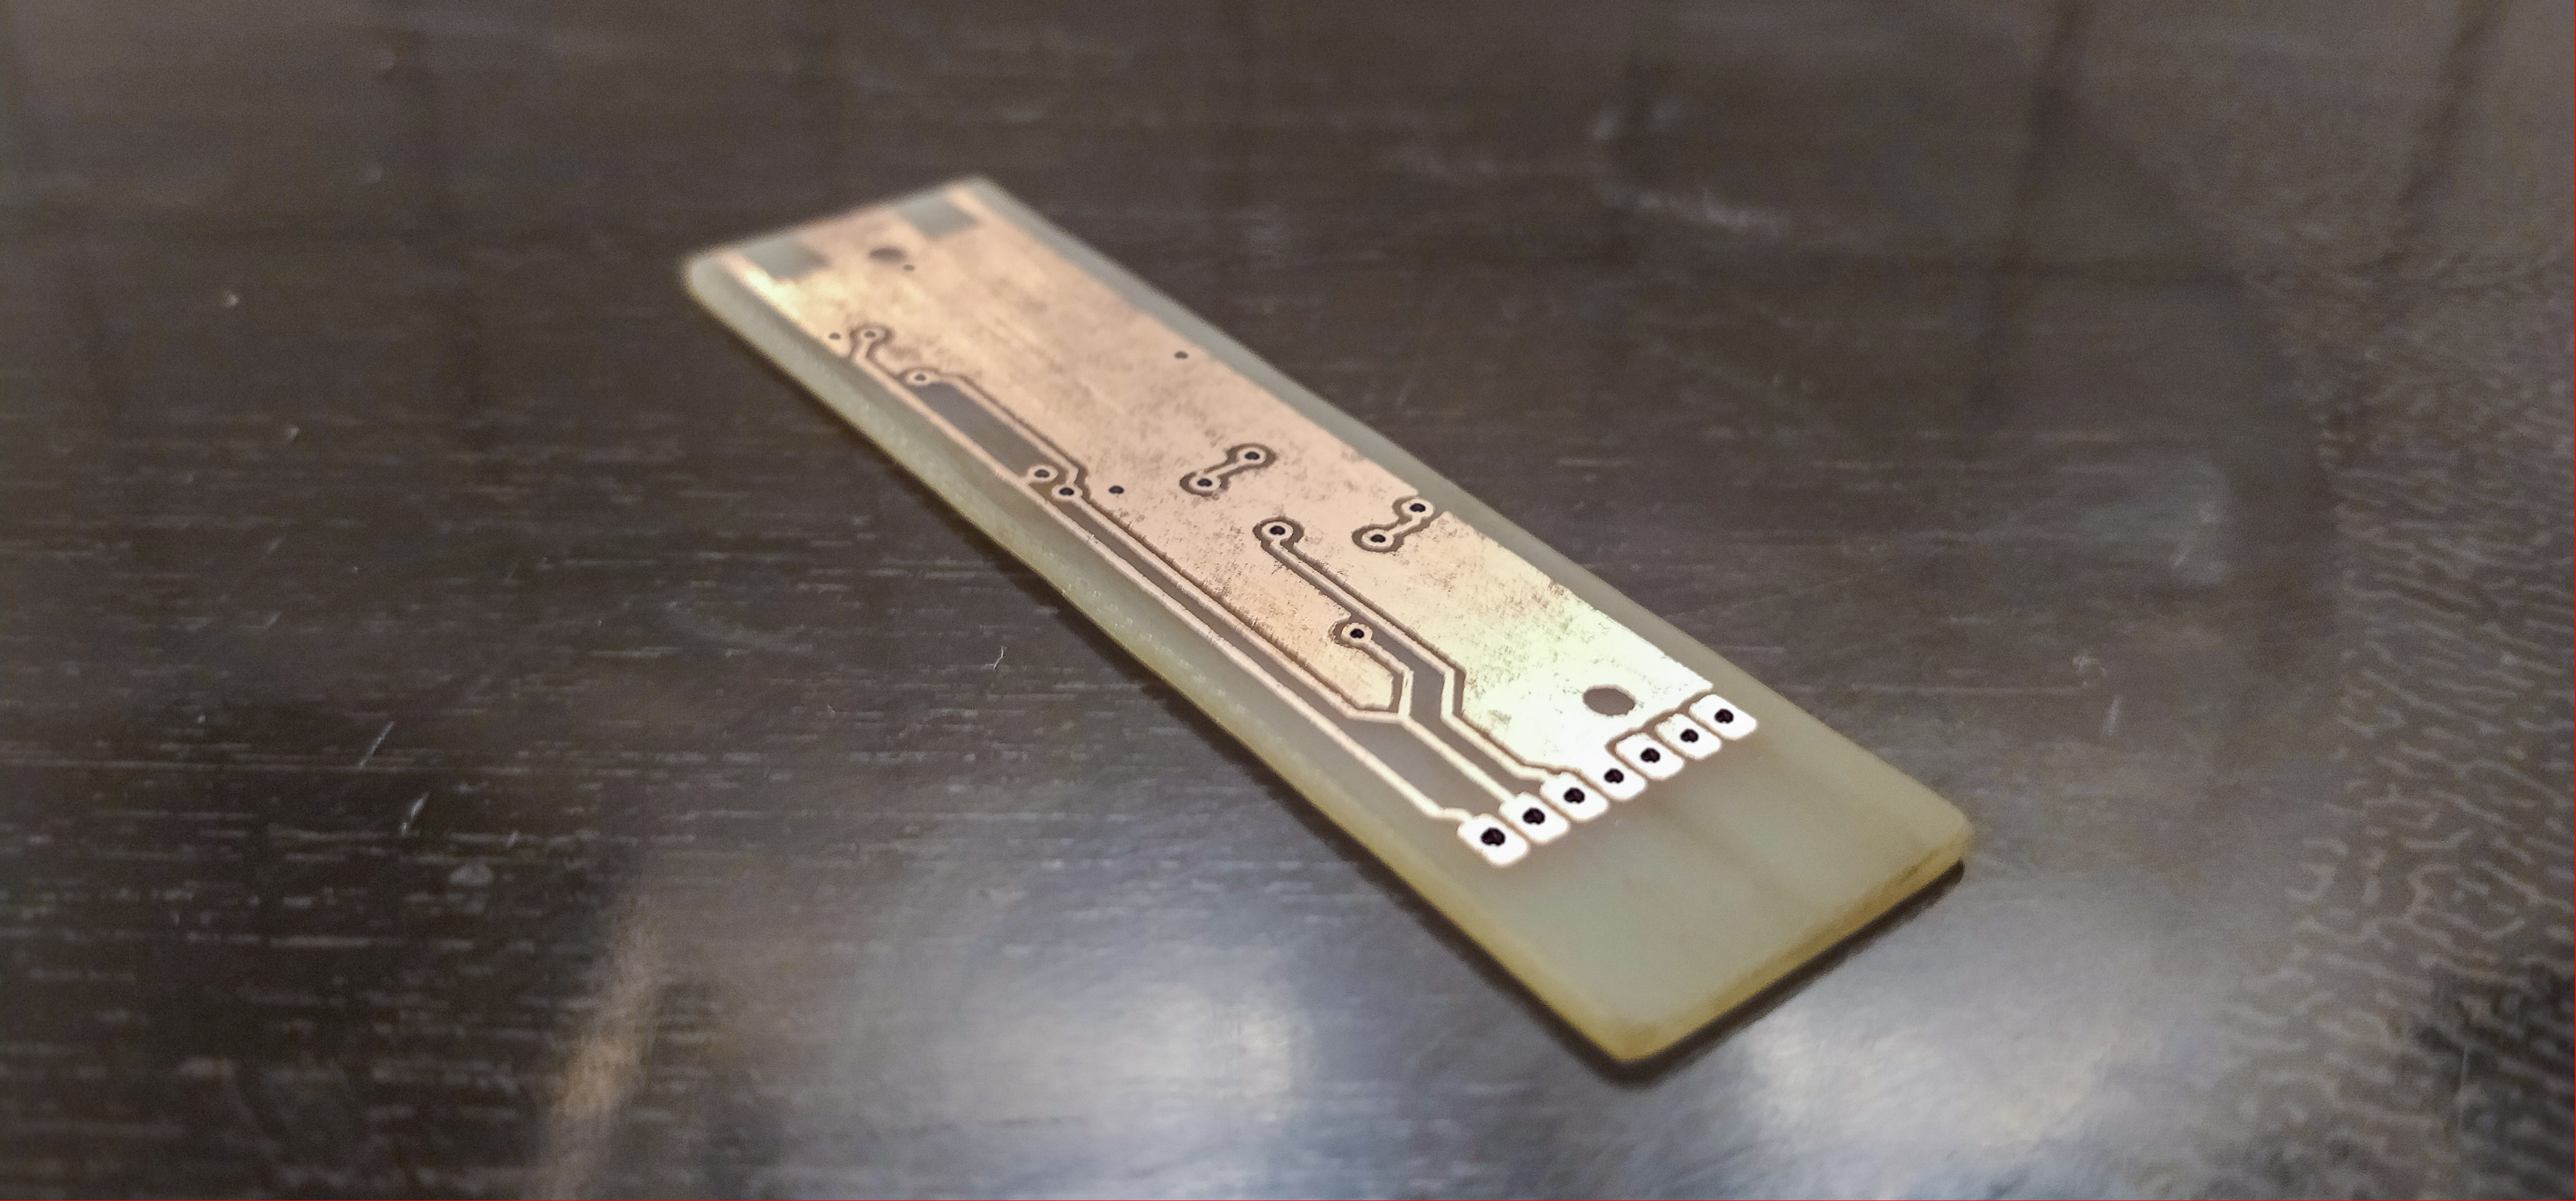
\includegraphics[width=\linewidth]{media/album/PSX_20220301_054445.jpg}
            \caption{}
            \label{fig:PhotoPCBPrepareDone}
        \end{minipage}
    \end{figure}

    Следующий этап --- пайка\footnote{Рисунки \ref{fig:PhotoPCBProgress1}, \ref{fig:PhotoPCBProgress2}, \ref{fig:PhotoPCBProgress3}, \ref{fig:PhotoCableProgress4}, \ref{fig:PhotoCableProgress5}} схемы, и здесь в дело вступает мелкая моторика.
    % TRANSLATOR NOTE: "antiossidante" (antioxidant) translated as "флюс" (flux), which is what is meant in soldering.
    Единственный совет, который я могу дать, --- обращать внимание на используемый флюс, поскольку некоторые флюсы проводят ток и, если их не удалить полностью\footnote{У SMD-компонентов его не удаётся убрать из-под припаянного элемента} после пайки, могут вызвать сбои.
    \begin{figure}[H]
        \centering
        \begin{minipage}[H]{.45\linewidth}
            \centering
            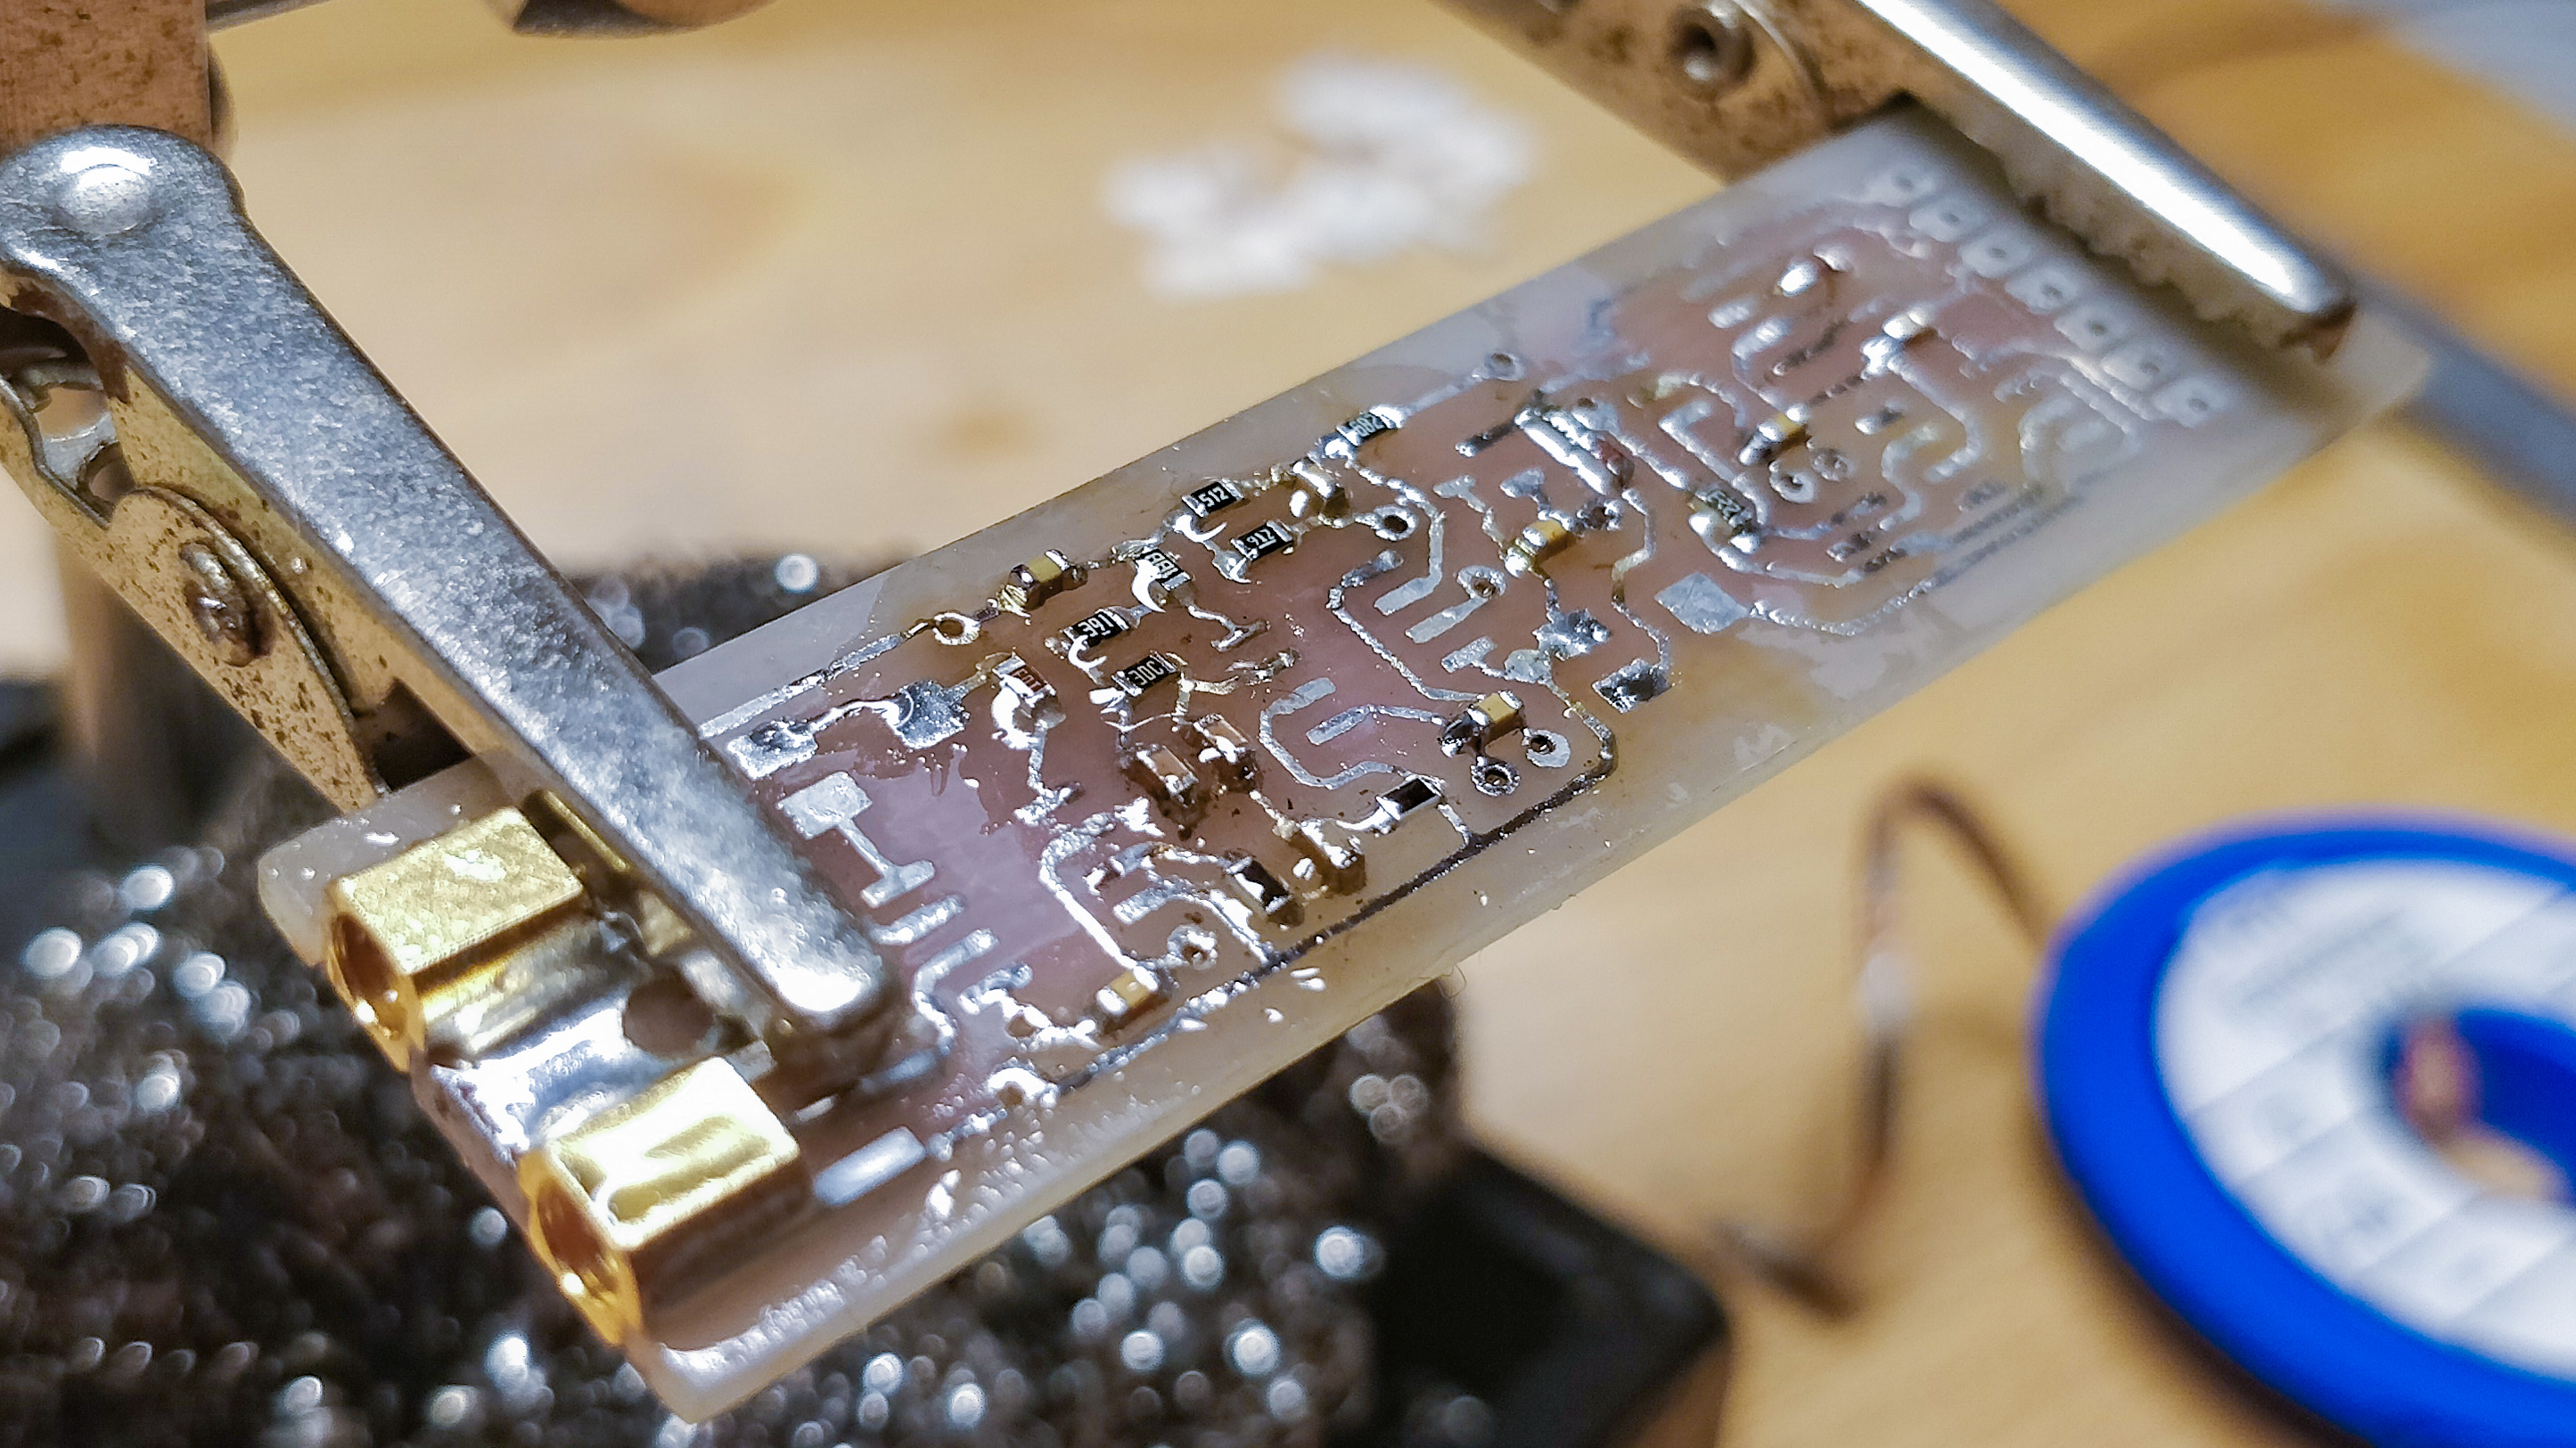
\includegraphics[width=\linewidth]{media/album/PSX_20220228_161847.jpg}
            \caption{}
            \label{fig:PhotoPCBProgress1}
        \end{minipage}
        \hspace{.04\linewidth}
        \begin{minipage}[H]{.45\linewidth}
            \centering
            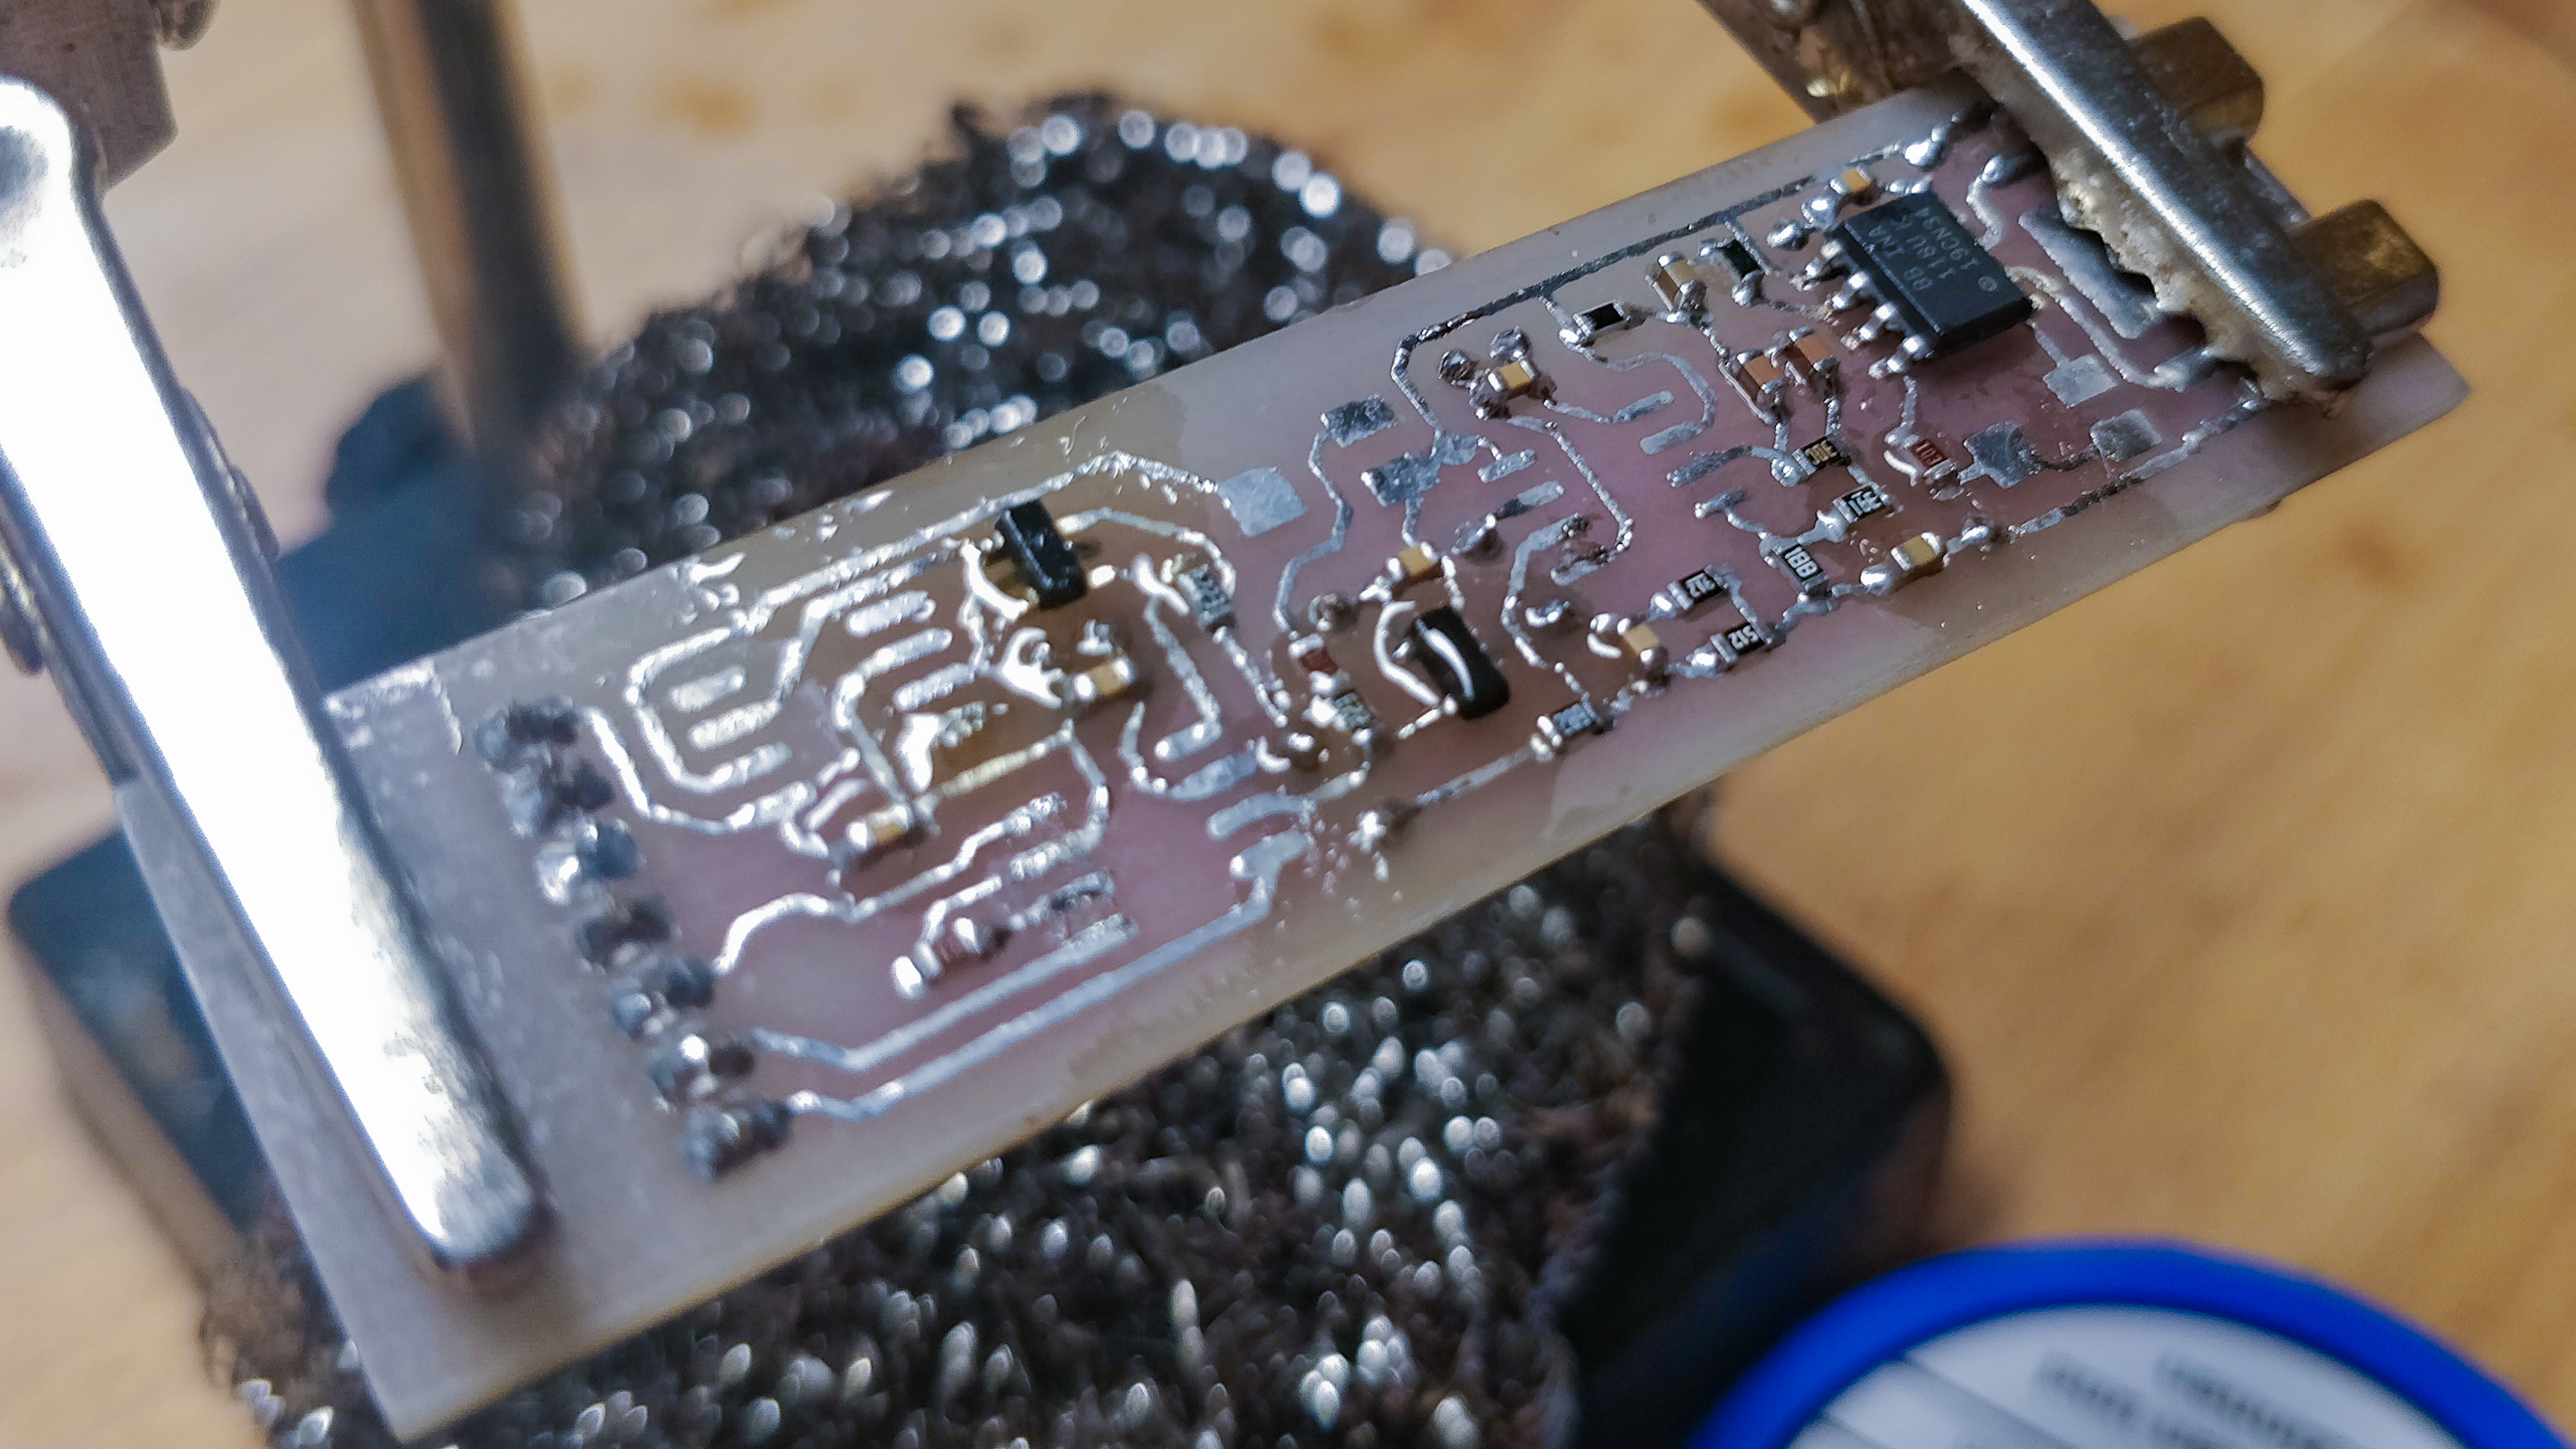
\includegraphics[width=\linewidth]{media/album/PSX_20220228_162014.jpg}
            \caption{}
            \label{fig:PhotoPCBProgress2}
        \end{minipage}
        \\
        \vspace*{.01\linewidth}
        \begin{minipage}[H]{.95\linewidth}
            \centering
            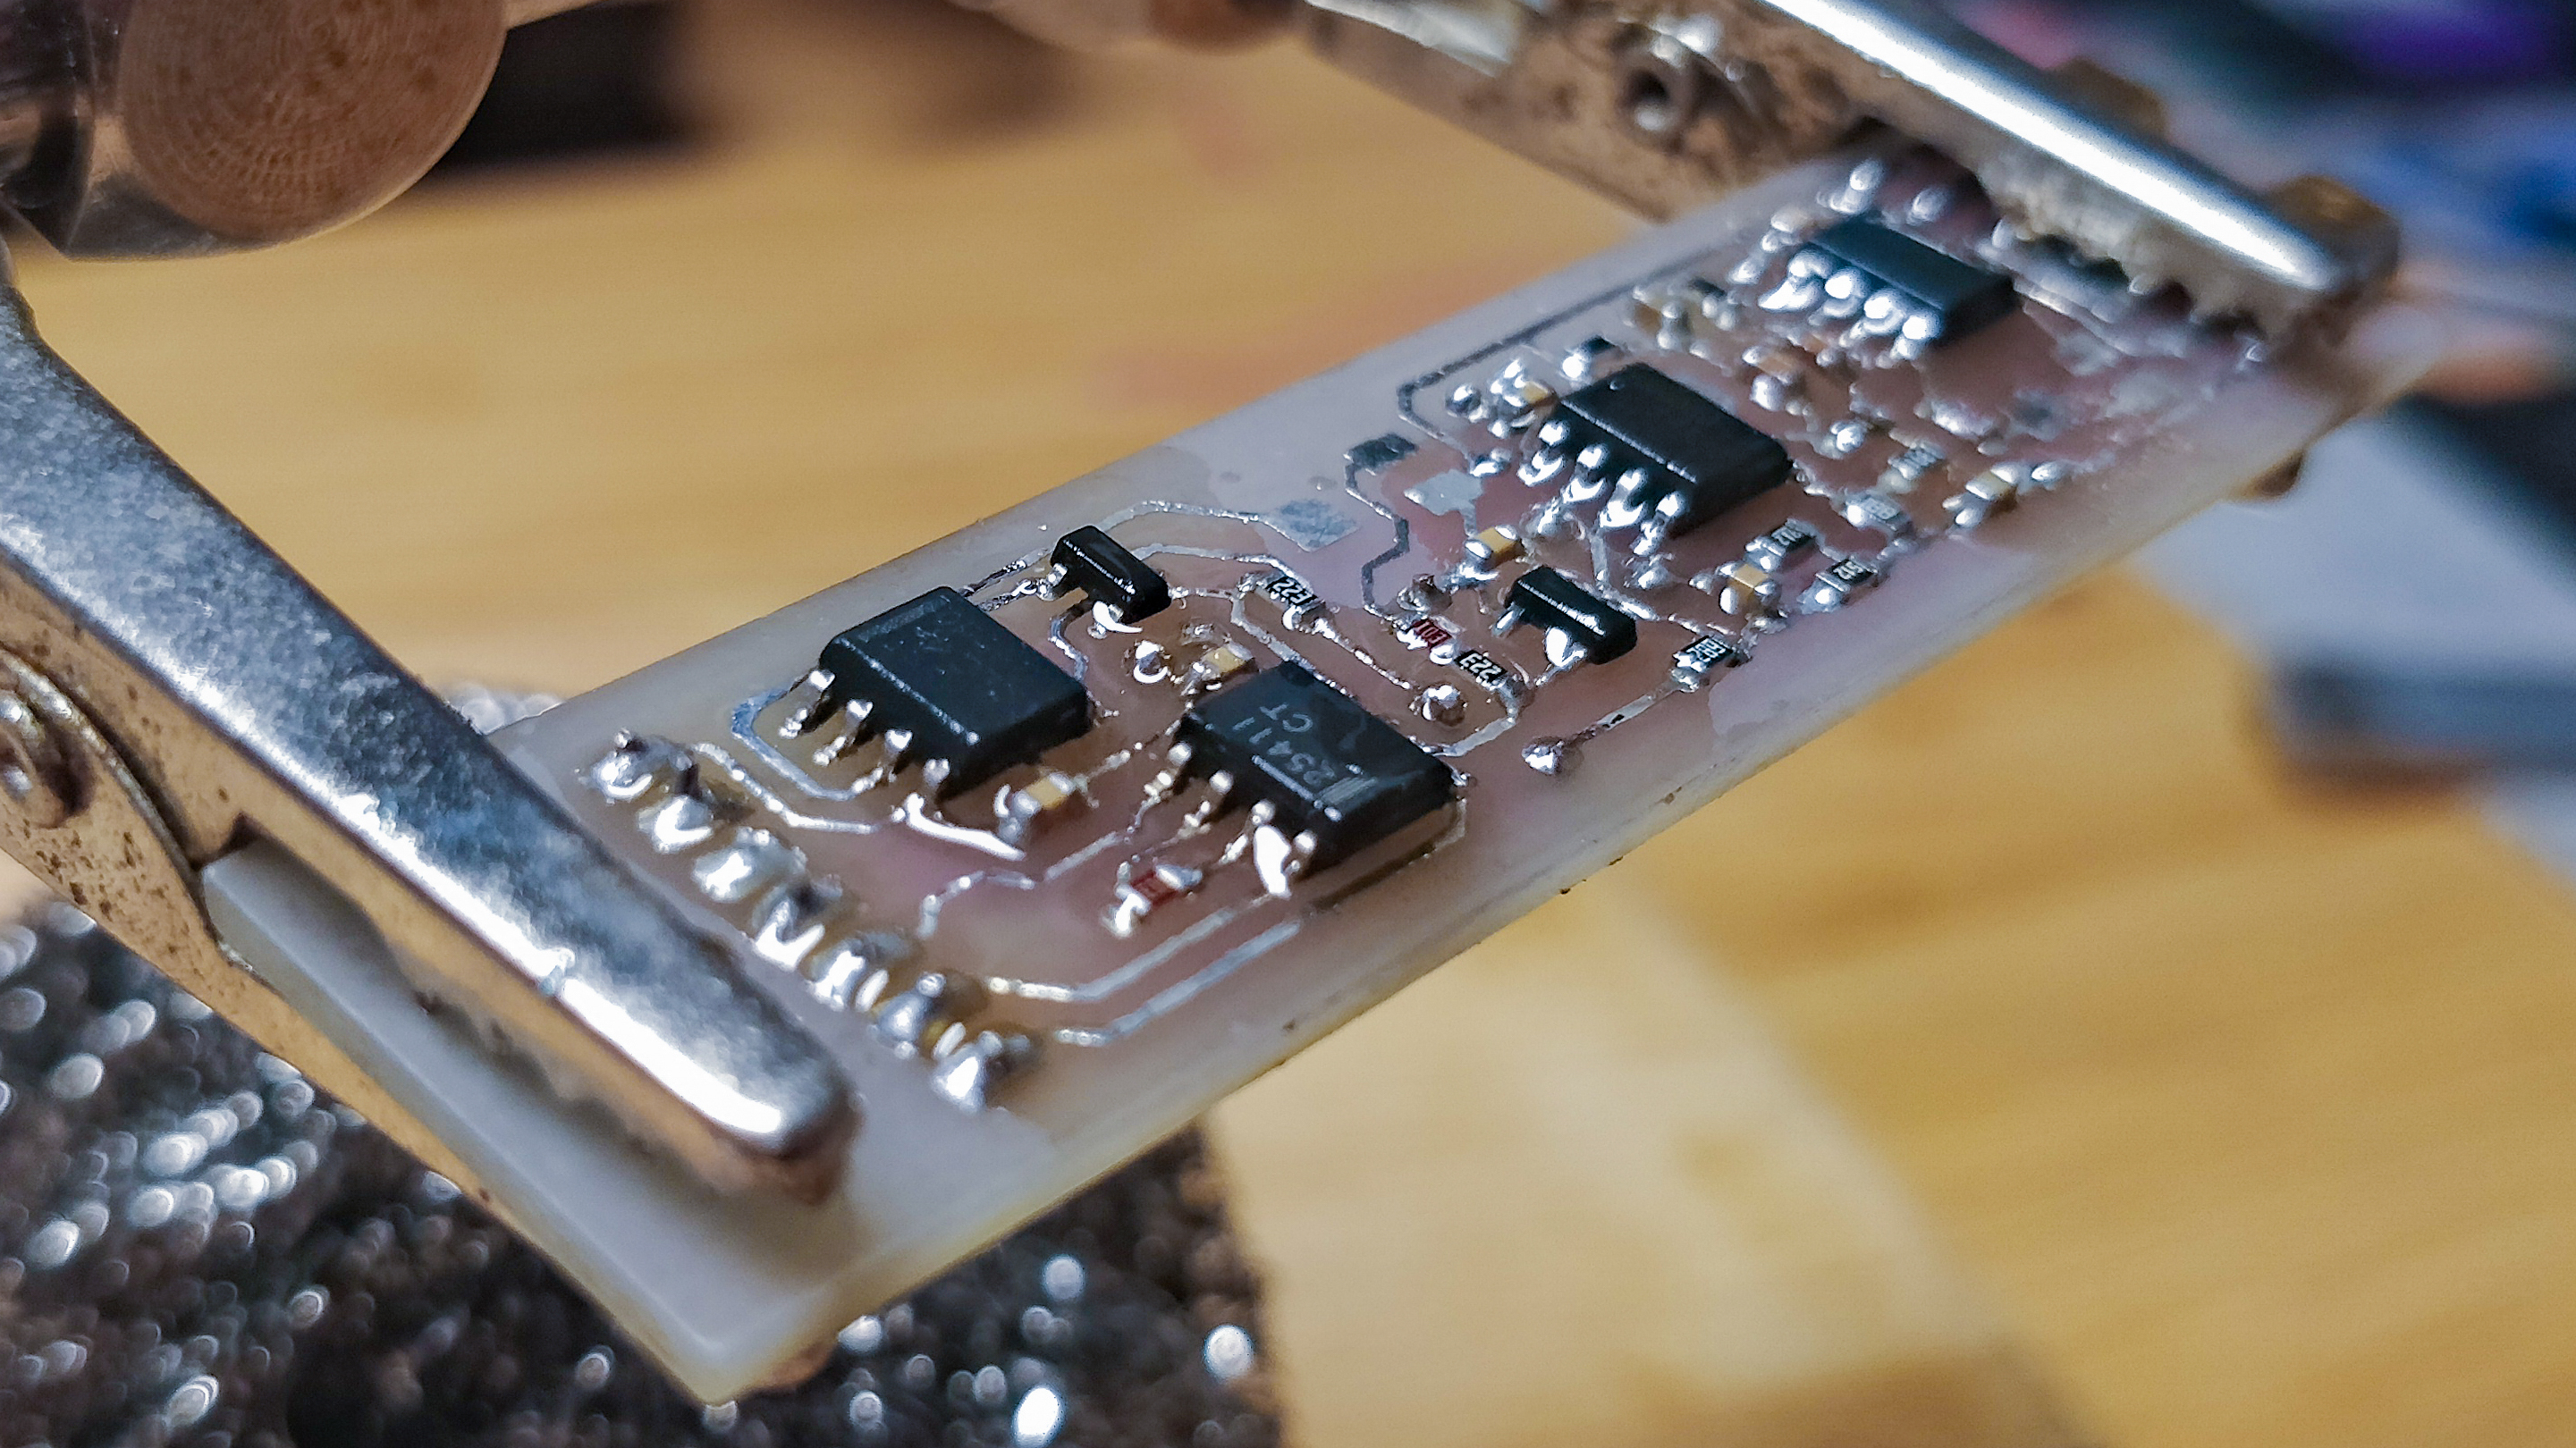
\includegraphics[width=\linewidth]{media/album/PSX_20220301_044735.jpg}
            \caption{}
            \label{fig:PhotoPCBProgress3}
        \end{minipage}
        \\
        \vspace*{.01\linewidth}
        \begin{minipage}[H]{.95\linewidth}
            \centering
            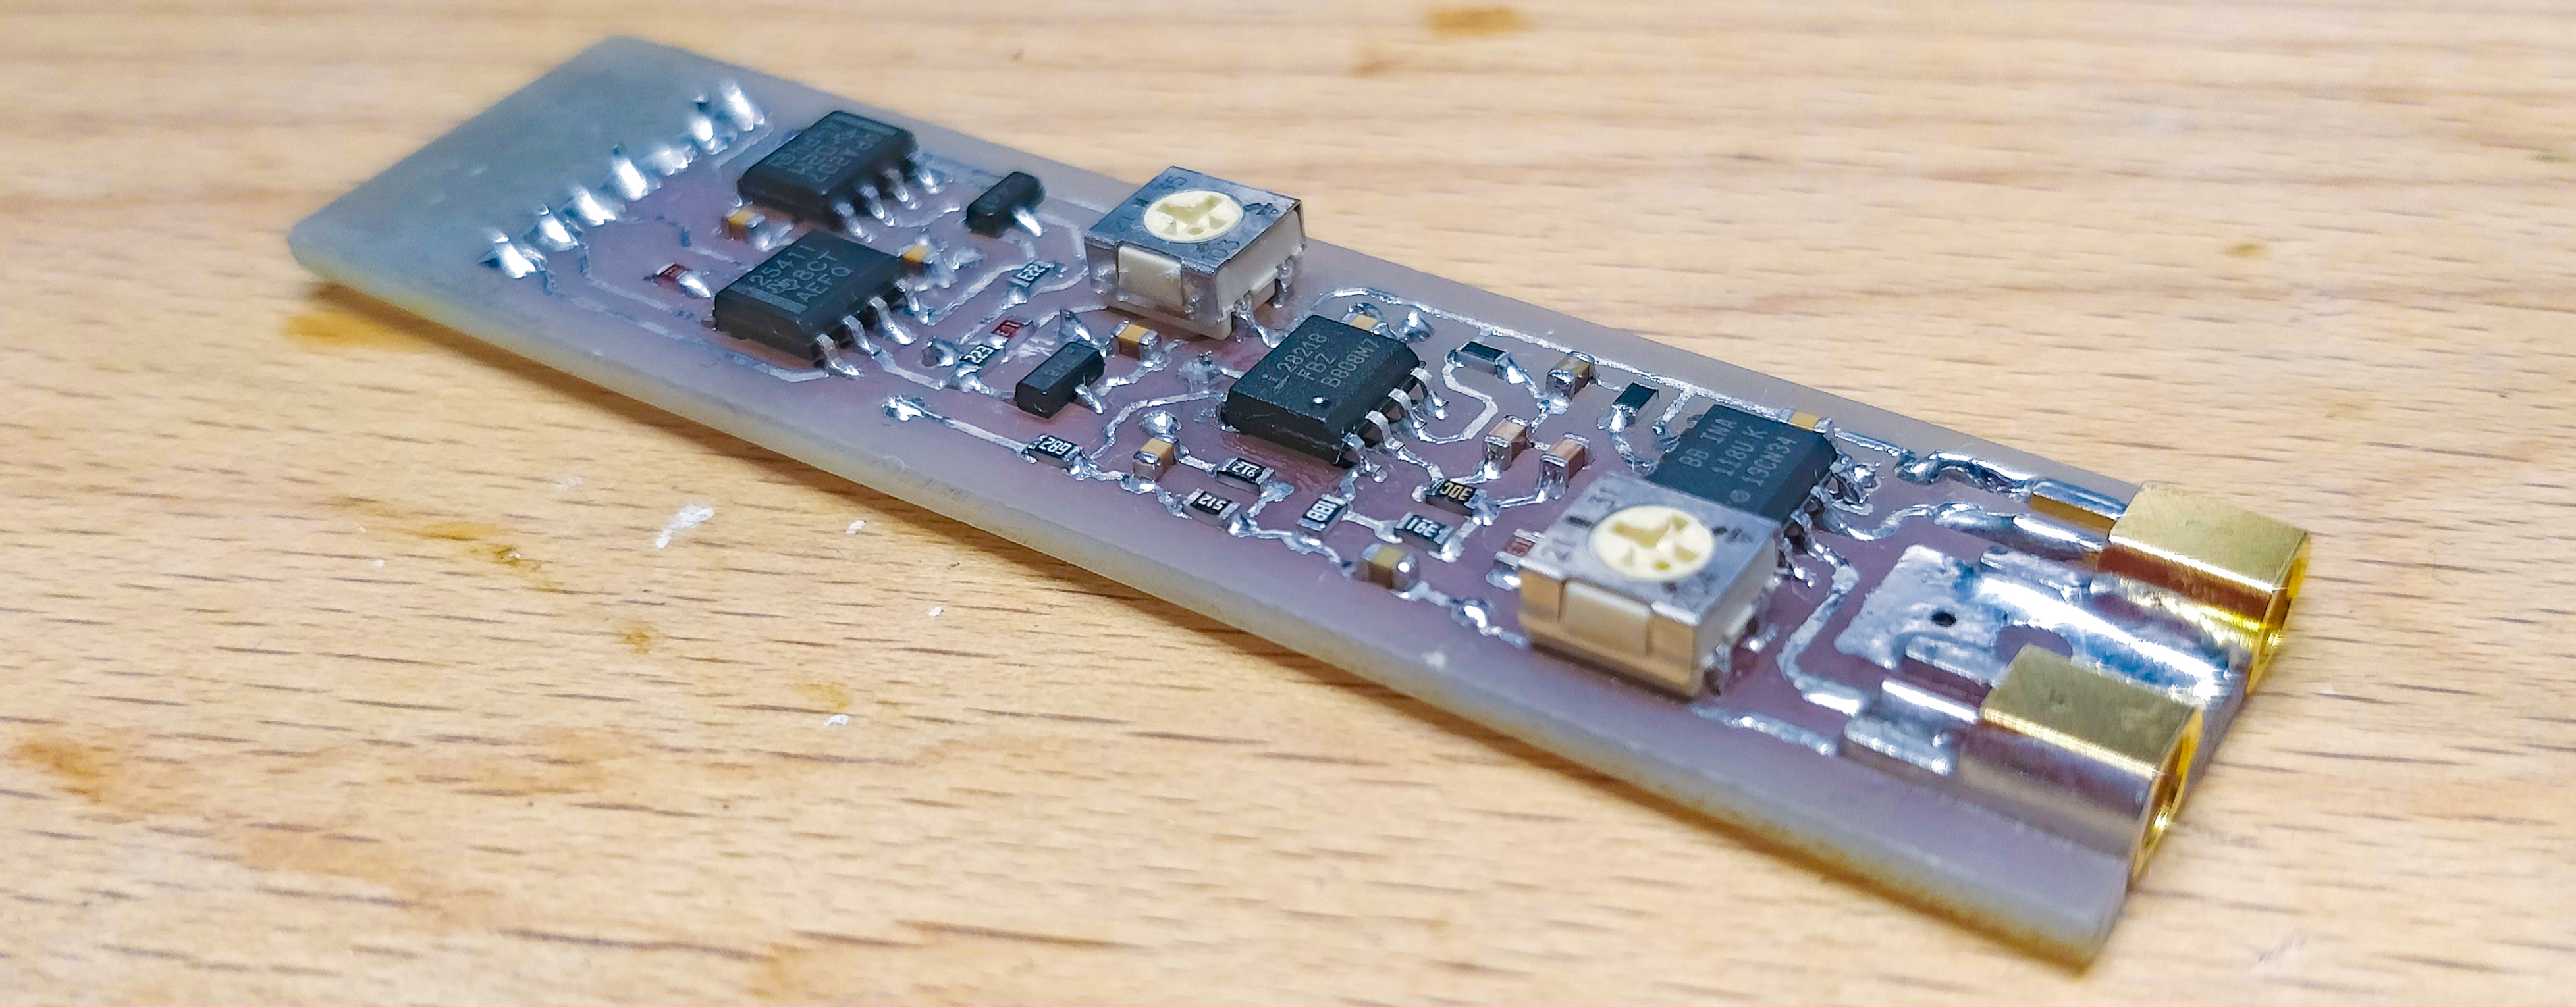
\includegraphics[width=\linewidth]{media/album/PSX_20220228_020356.jpg}
            \caption{}
            \label{fig:PhotoPCBDone}
        \end{minipage}
    \end{figure}

    Из-за небольшой ошибки в заказе я не смог впаять разъём $J3$, поэтому вместо него припаял провода. После пайки кабелей\footnote{Рисунки \ref{fig:PhotoCableProgress1}, \ref{fig:PhotoCableProgress2}, \ref{fig:PhotoCableProgress3}, \ref{fig:PhotoCableProgress4}, \ref{fig:PhotoCableProgress5}, \ref{fig:PhotoCableDone}} электродов схема была готова.
    \begin{figure}[H]
        \RaggedRight
        \centering   
        \begin{minipage}[H]{.95\linewidth}
            \centering
            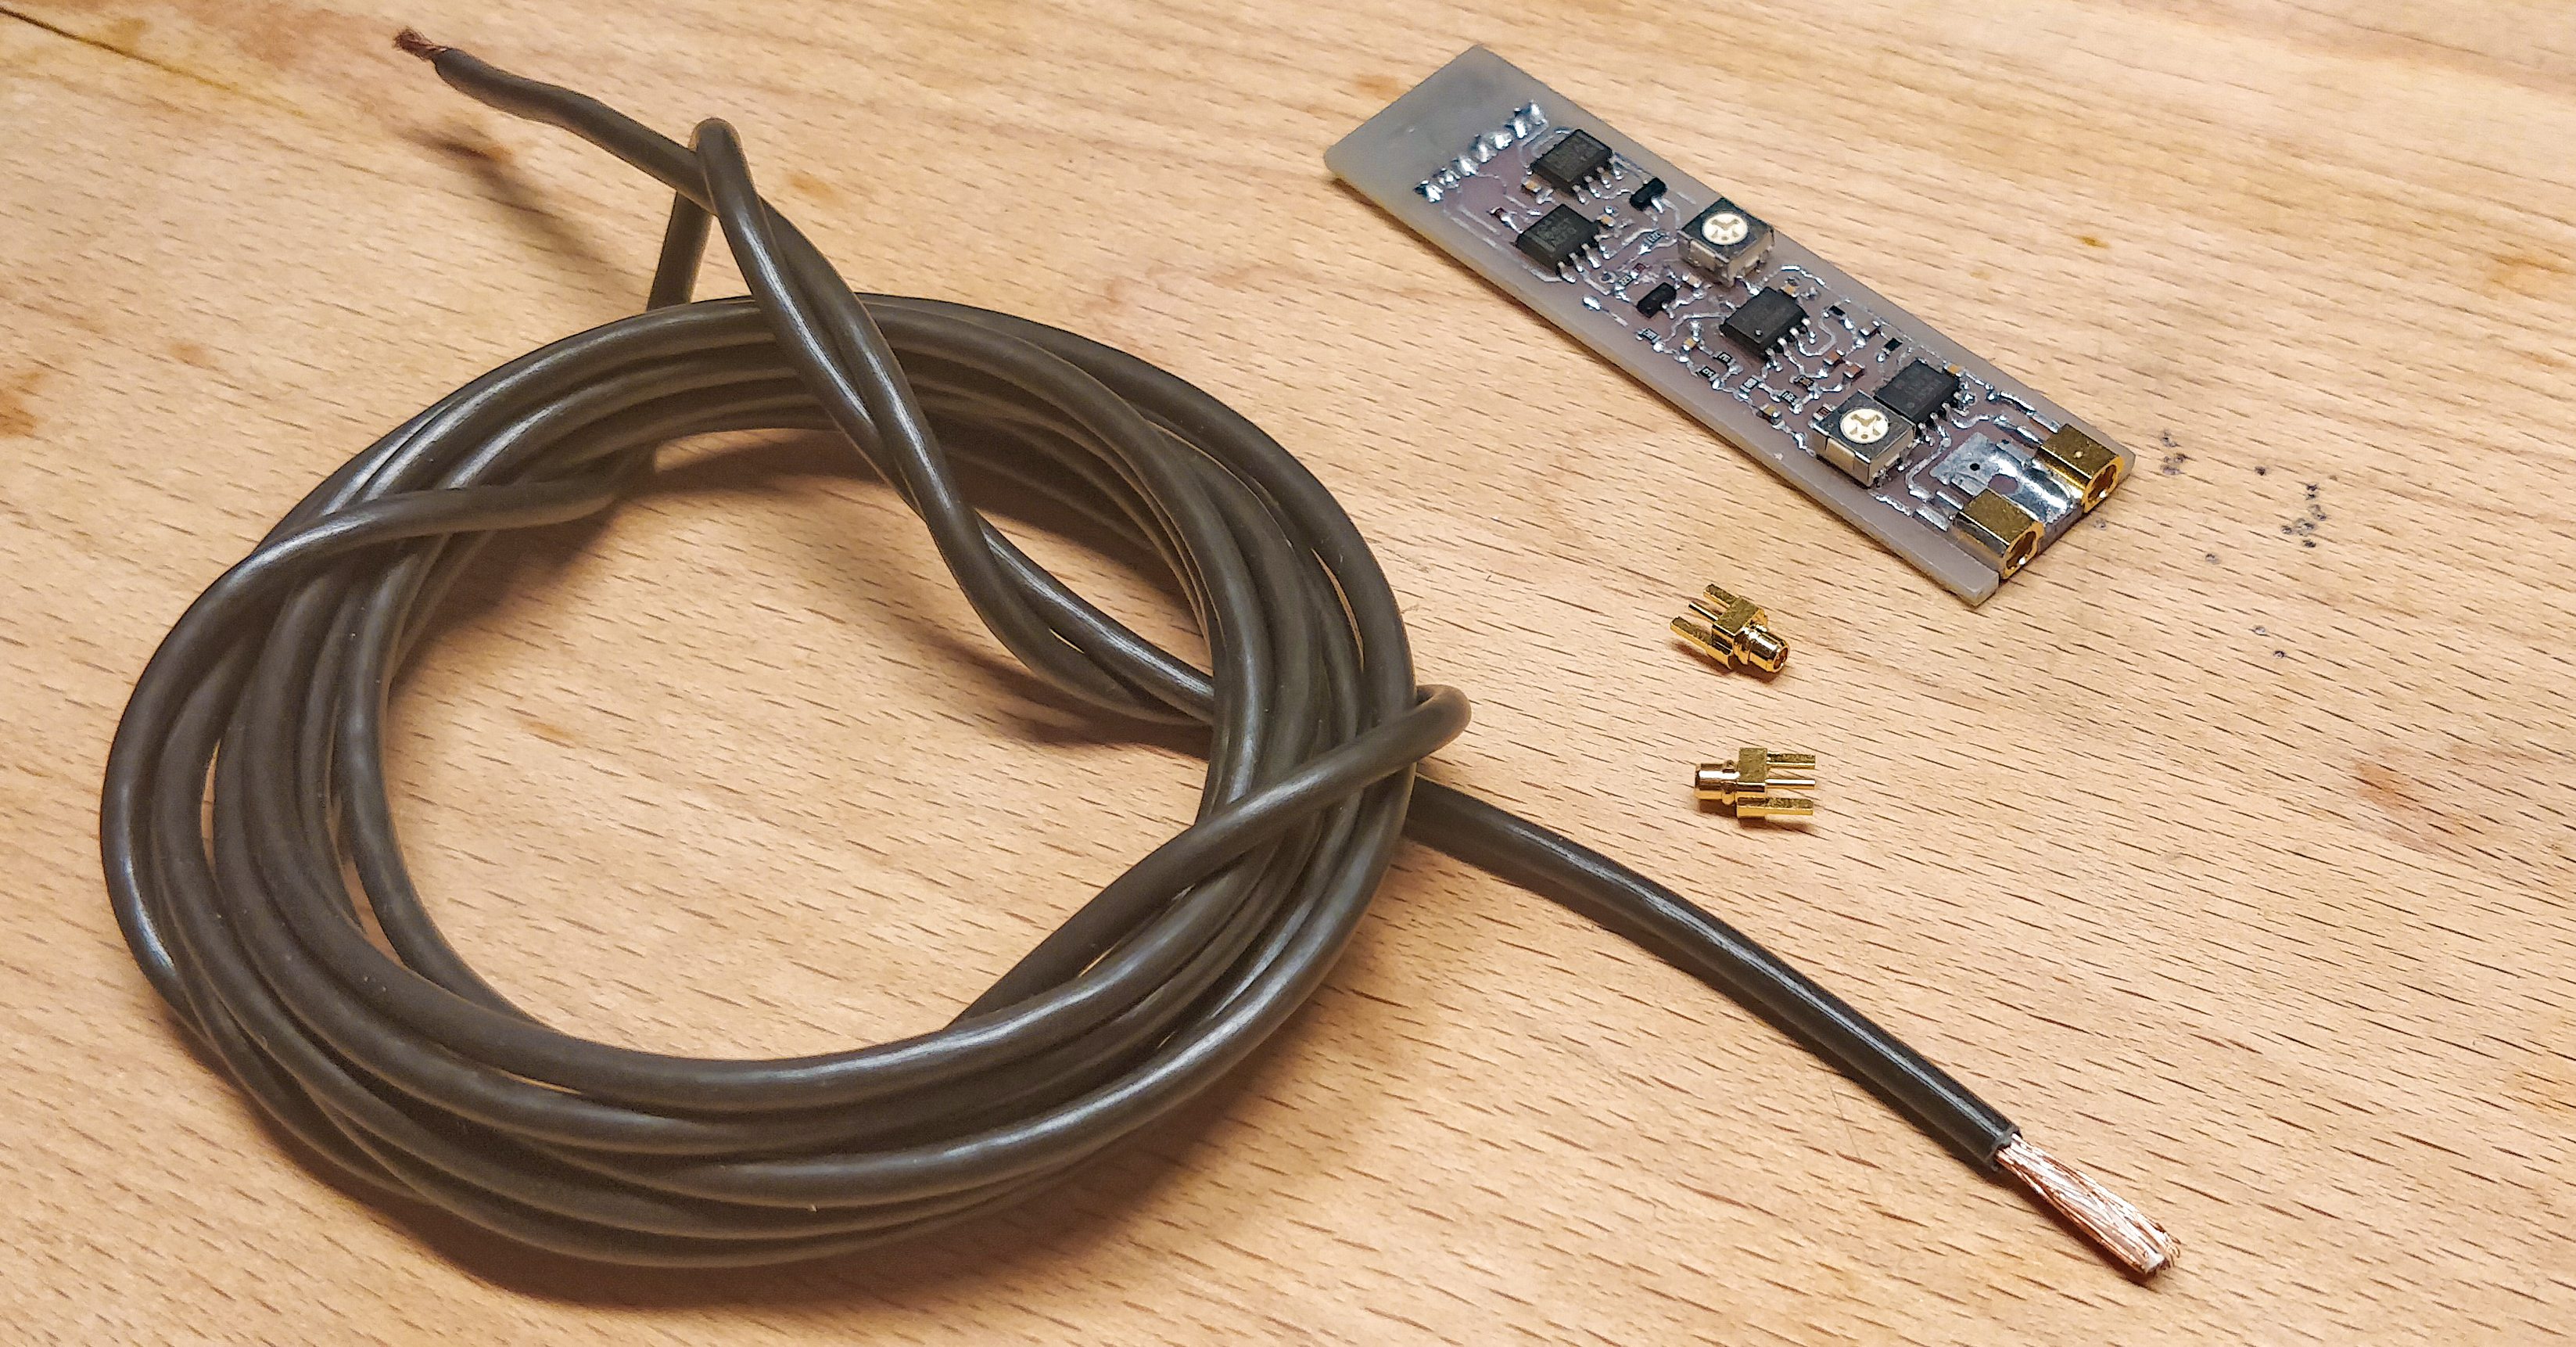
\includegraphics[width=\linewidth]{media/album/PSX_20220228_020856.jpg}
            \caption{}
            \label{fig:PhotoCableProgress1}
        \end{minipage}
        \\
        \vspace*{.01\linewidth}
        \begin{minipage}[H]{.28\linewidth}
            \centering
            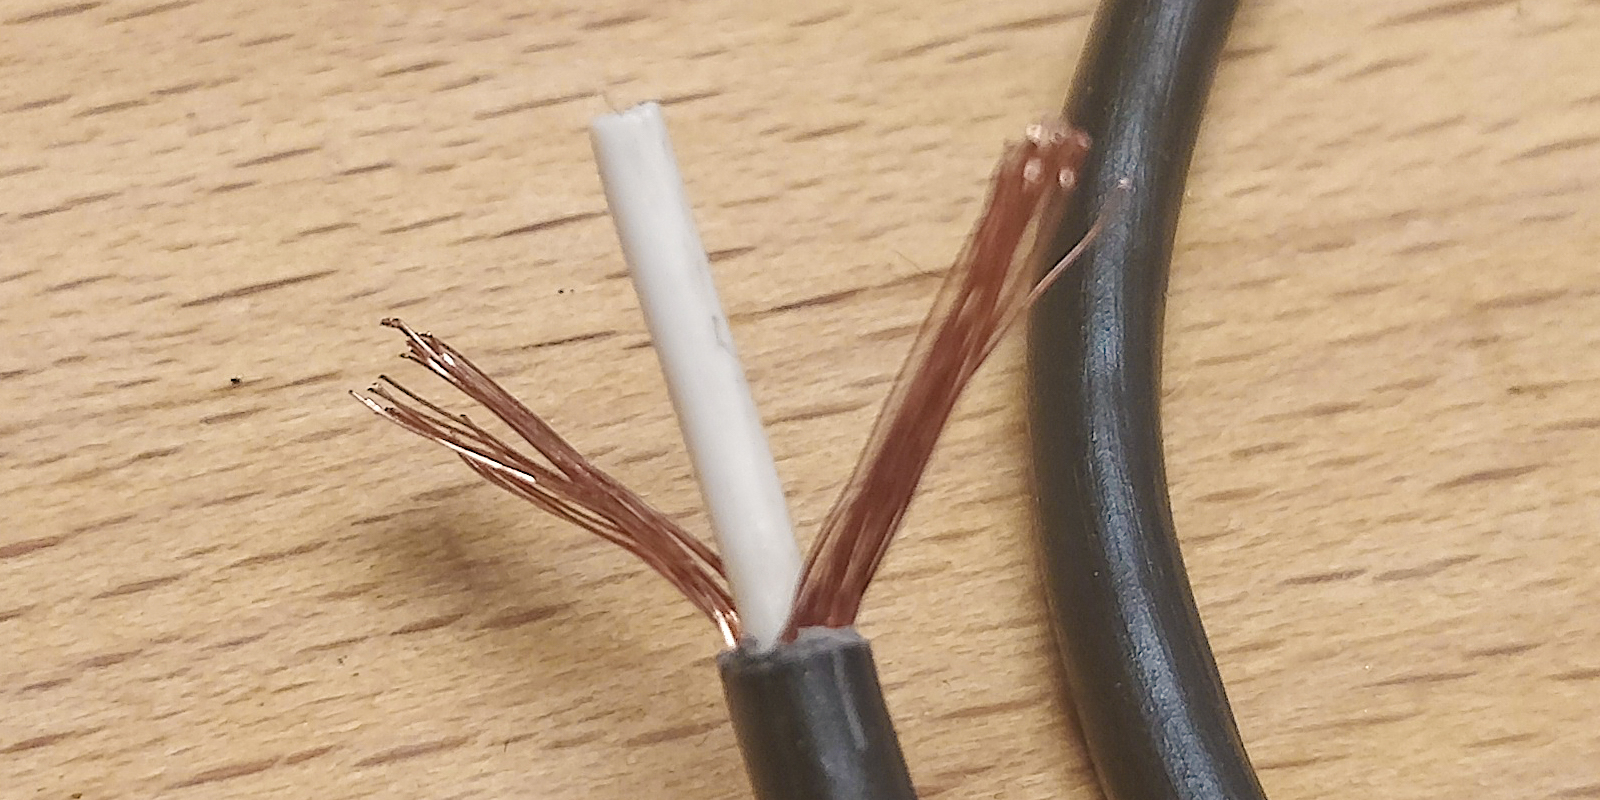
\includegraphics[width=\linewidth]{media/album/PSX_20220228_020741.jpg}
            \caption{}
            \label{fig:PhotoCableProgress2}
        \end{minipage}
        \hspace{.04\linewidth}
        \begin{minipage}[H]{.28\linewidth}
            \centering
            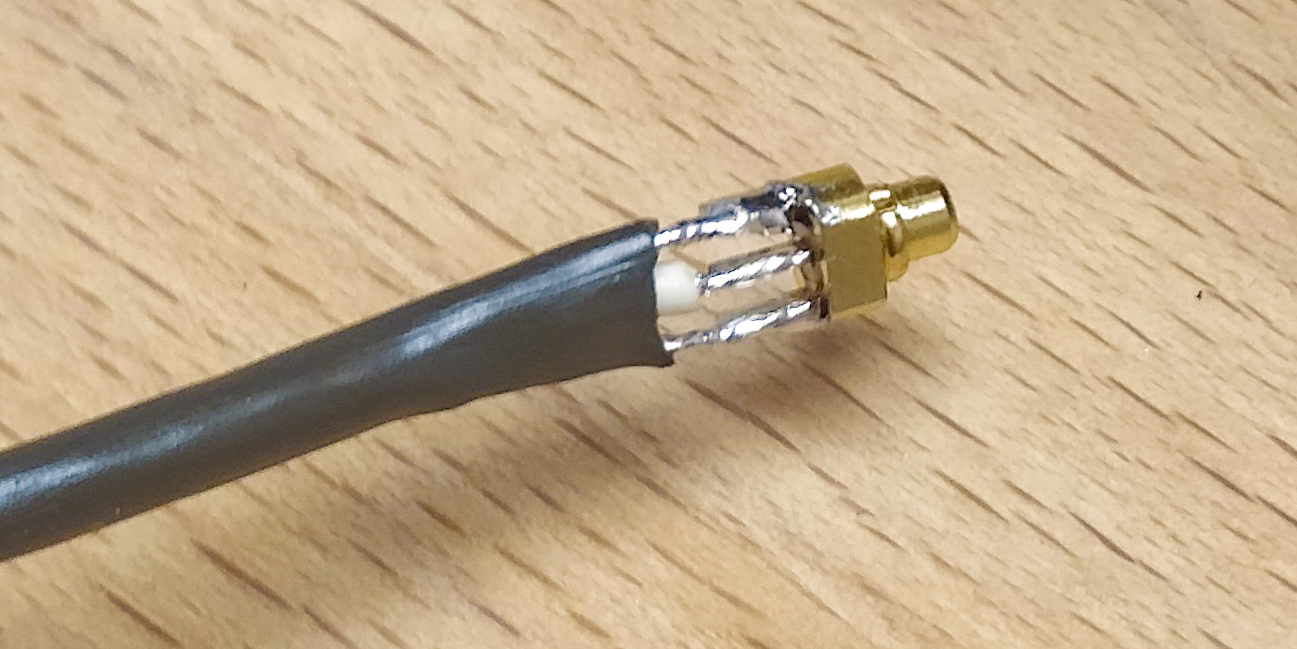
\includegraphics[width=\linewidth]{media/album/PSX_20220228_162153.jpg}
            \caption{}
            \label{fig:PhotoCableProgress3}
        \end{minipage}
        \hspace{.04\linewidth}
        \begin{minipage}[H]{.28\linewidth}
            \centering
            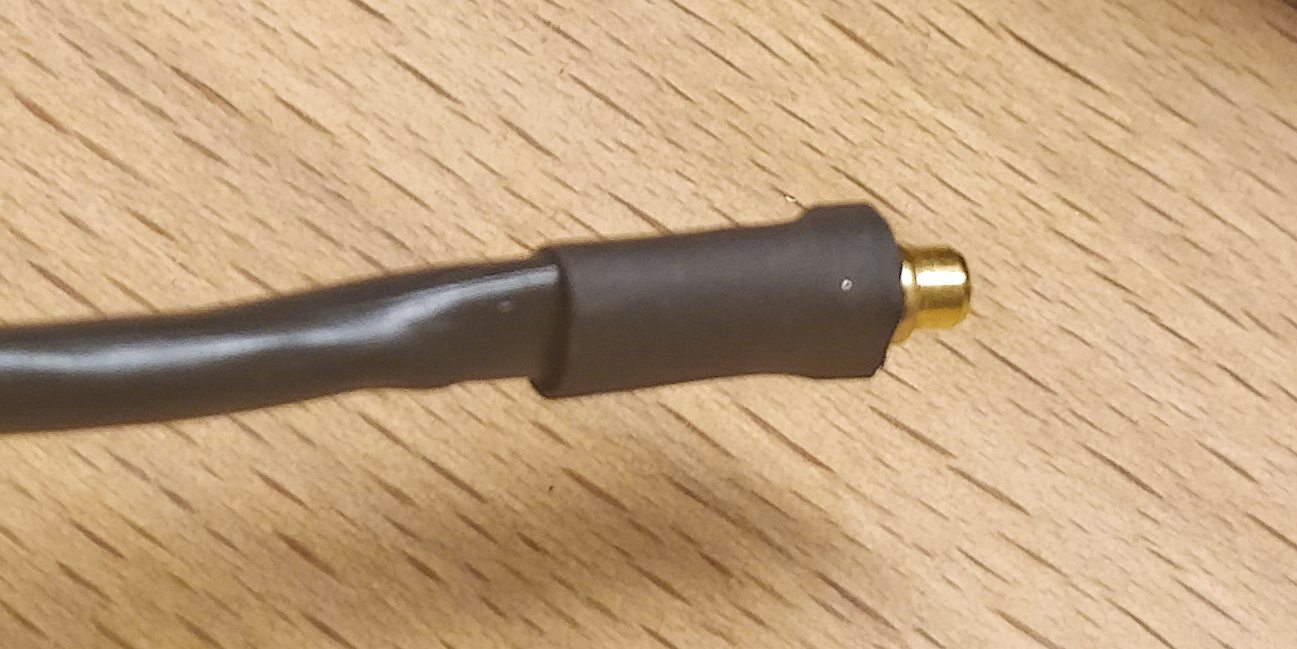
\includegraphics[width=\linewidth]{media/album/PSX_20220228_162233.jpg}
            \caption{}
            \label{fig:PhotoCableProgress4}
        \end{minipage}
        \\
        \vspace*{.01\linewidth}
        \begin{minipage}[H]{.95\linewidth}
            \centering
            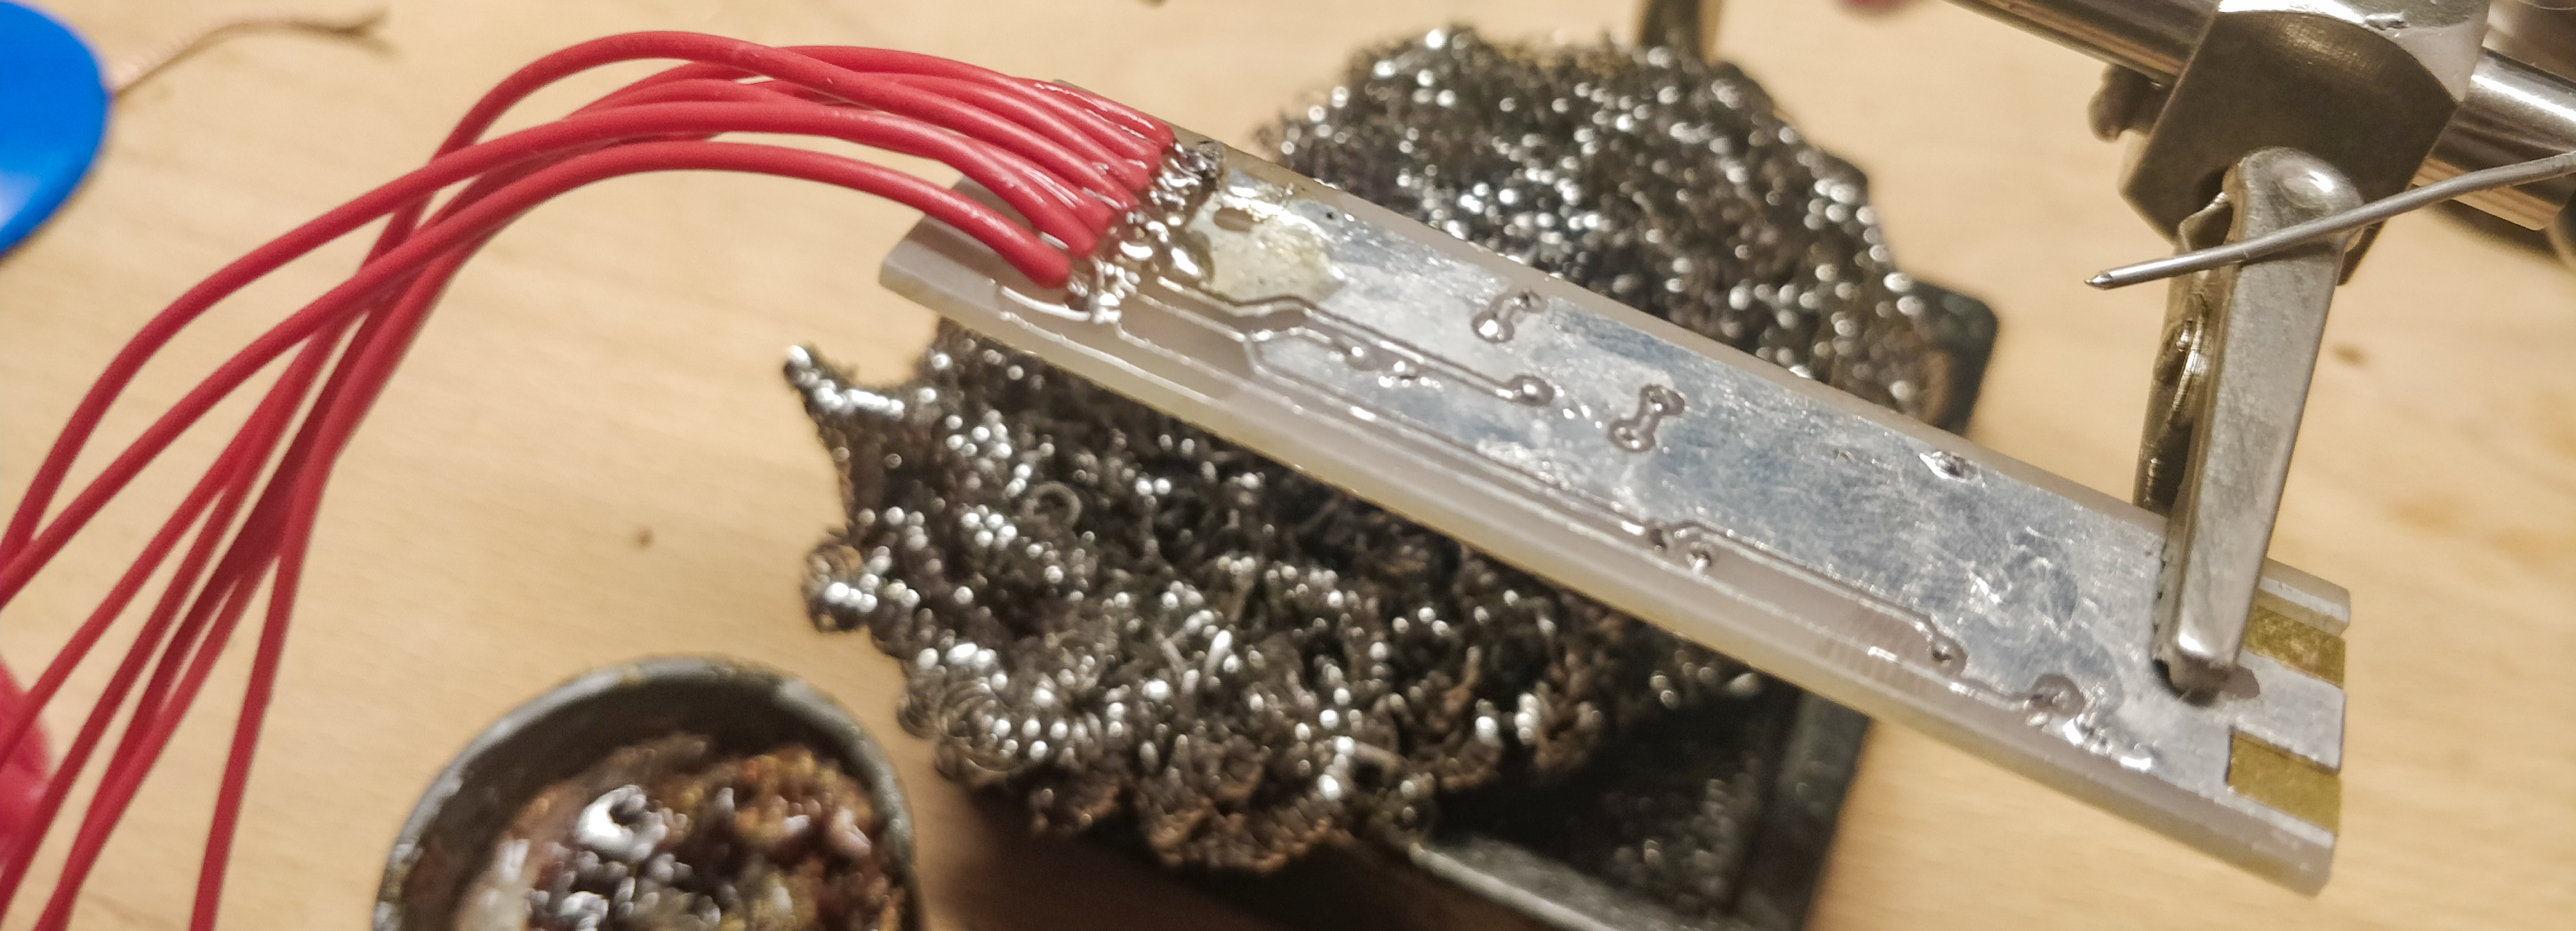
\includegraphics[width=\linewidth]{media/album/PSX_20220228_020557.jpg}
            
            \caption{}
            \label{fig:PhotoCableProgress5}
        \end{minipage}
        \\
        \vspace*{.01\linewidth}
        \begin{minipage}[H]{.95\linewidth}
            \centering
            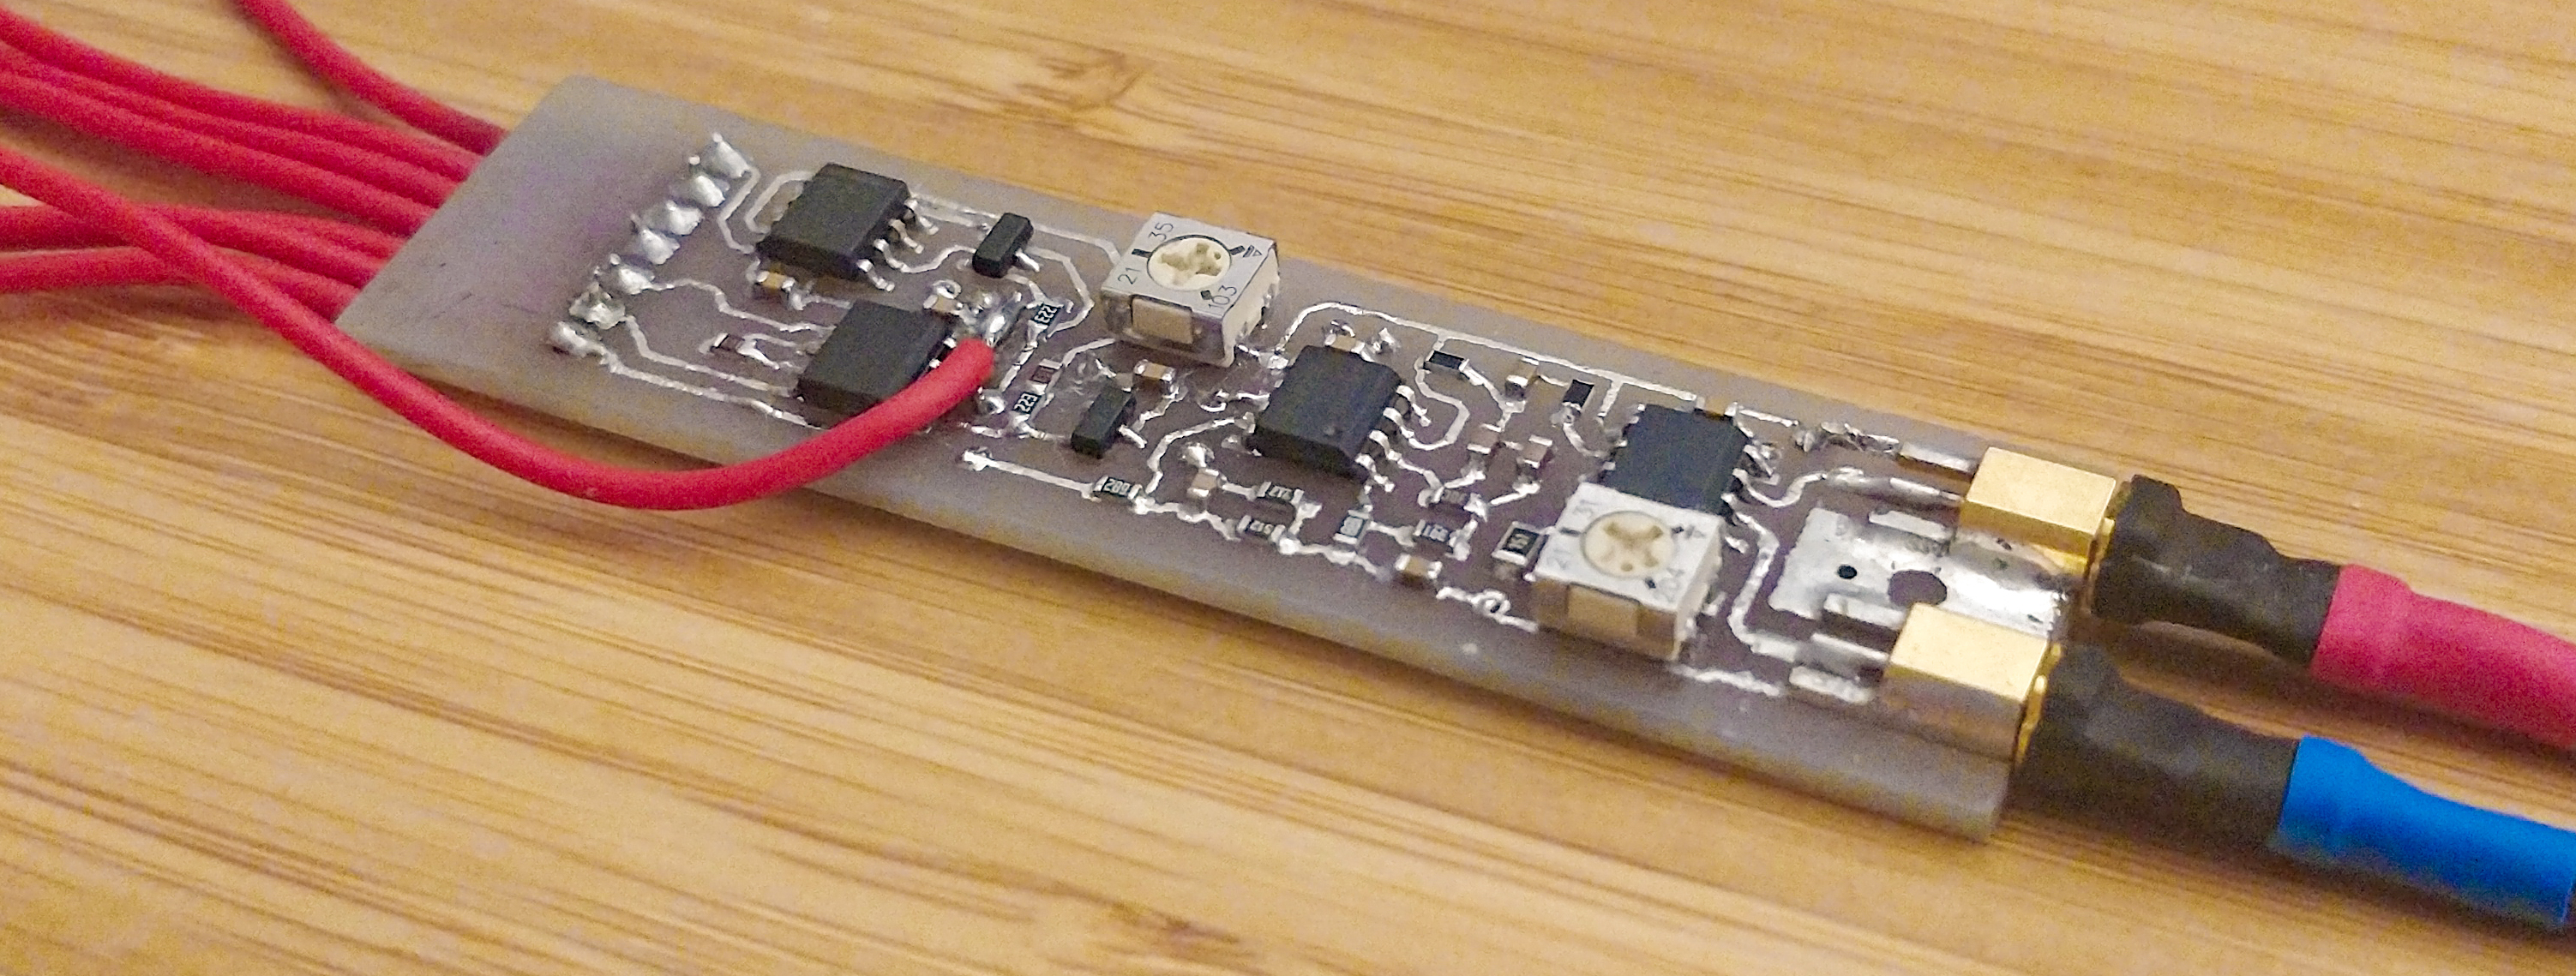
\includegraphics[width=\linewidth]{media/album/PSX_20220227_234925.jpg}
            \caption{}
            \label{fig:PhotoCableDone}
        \end{minipage}
    \end{figure}


    \subsection{Подключение}
    Я подключил схему так, как было предусмотрено схемой:
    \begin{center}
    \begin{tabular}{ ||l|l|| }
        \hline
        \multicolumn{1}{||l|}{Сенсорная плата} & \multicolumn{1}{|l||}{Arduino Due \& стабилизатор} \\
        \hline
        \hline
        CS\footnote{Chip Select, выбор микросхемы} & вывод 4\footnote{Подойдёт любой цифровой вывод}\\
        \hline
        SDO\footnote{Serial Data Output, выход последовательных данных} & MISO\\
        \hline
        SCLK\footnote{Serial Clock, последовательный вывод, задающий ритм передачи данных} & SCLK\\
        \hline
        $5V$   & $5V$\\
        \hline
        $3V3$  & $3.3V$\\
        \hline
        $-3V3$ & $-3.3V$ (стабилизатор)\\
        \hline
        GND    & GND\\
        \hline
    \end{tabular}
    \end{center}
    \noindent И обнаружил, что АЦП не работает по неизвестной мне причине\footnote{SDO АЦП всё время оставался в «$0$»: $0-20mV$}.
    Тогда я решил использовать аналоговый вход Arduino DUE с 10-битным АЦП.

    \noindent Новое подключение следующее
    \begin{center}
        \begin{tabular}{ ||l|l|| }
            \hline
            \multicolumn{1}{||l|}{Сенсорная плата} & \multicolumn{1}{|l||}{Arduino Due \& стабилизатор} \\
            \hline
            \hline
            Выход каскада выпрямления\footnote{SEMG Sensor Board - RECT} & A0\footnote{Аналоговый вход Arduino DUE}\\
            \hline
            $5V$   & $5V$\\
            \hline
            $3V3$  & $3.3V$\\
            \hline
            $-3V3$ & $-3.3V$ (стабилизатор)\\
            \hline
            GND    & GND\\
            \hline
        \end{tabular}
    \end{center}

    \begin{figure}[H]
        \centering
        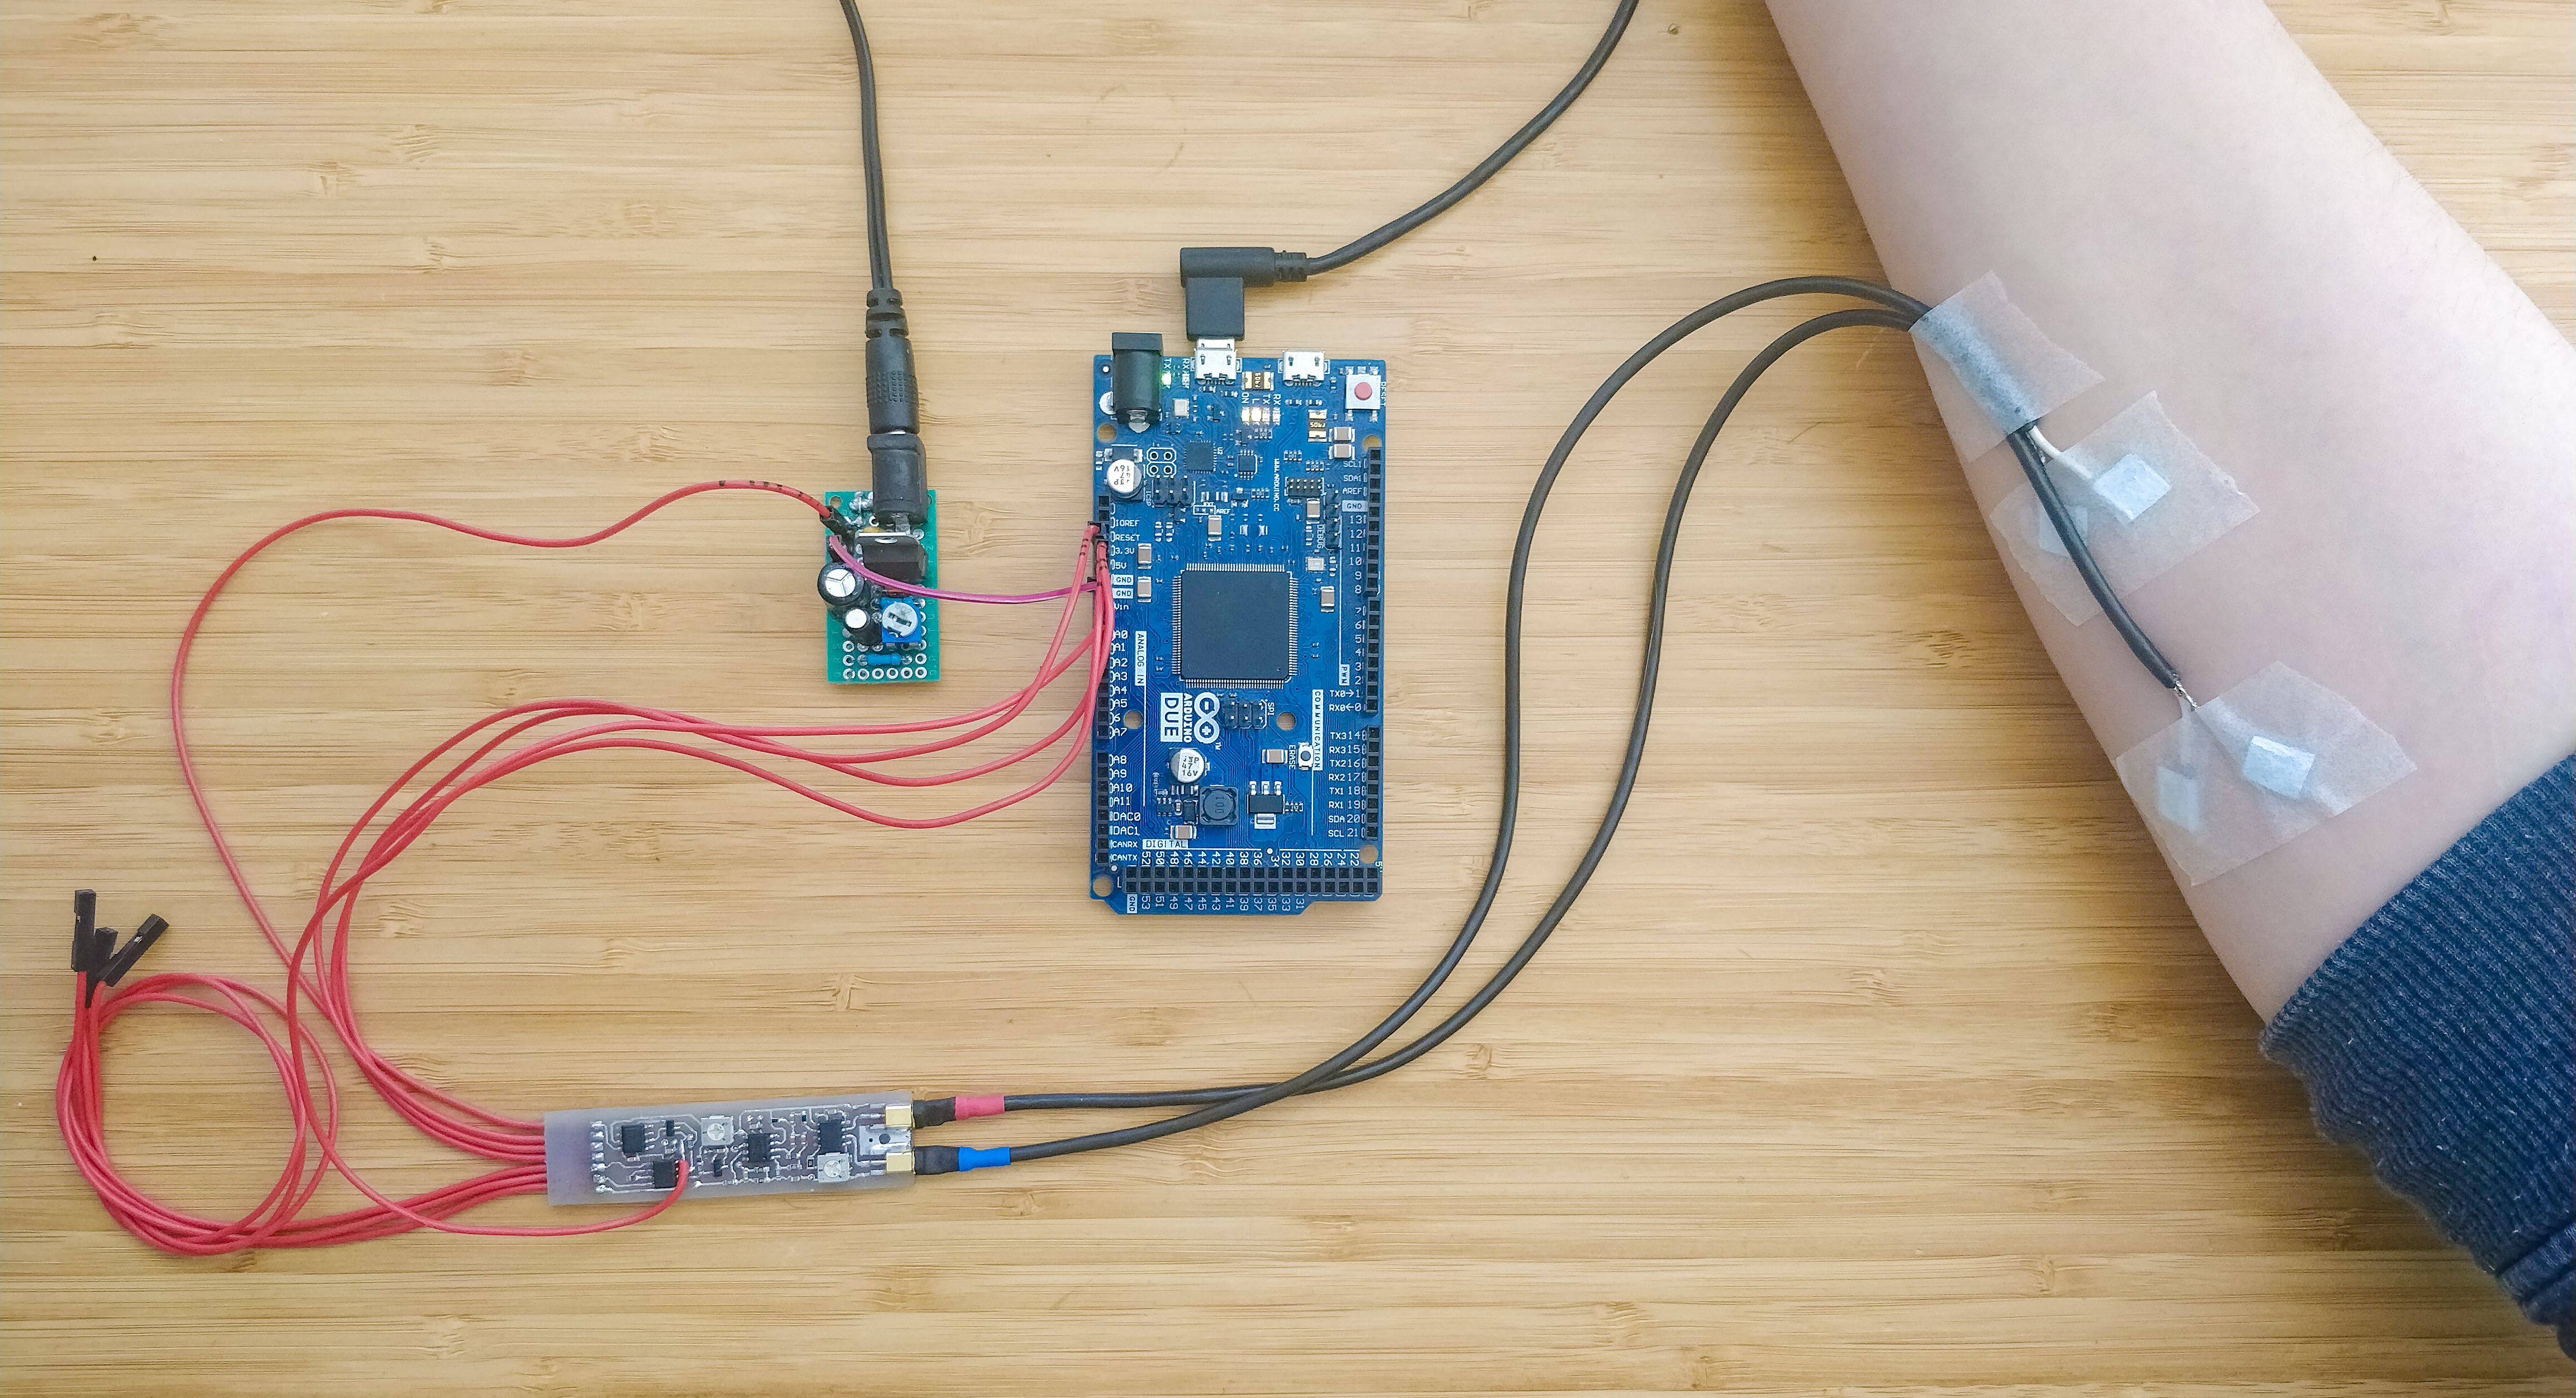
\includegraphics[width=\linewidth]{media/album/PSX_20220227_234659.jpg}
        \caption{Подключение всего прототипа}
        \label{fig:AllConnection}
    \end{figure}
    
    \subsection{Программное обеспечение}
    Код для обмена данными с АЦП по протоколу SPI:
    \begin{verbatim}
        #include <Arduino.h>            // Importa la libreria di Arudino
        #include <SPI.h>                // Importa la libreria del protocollo SPI

        /* --------------------- */
        #define SS_PIN_TLV2541  4       // Pin digitale connesso al Chip Select dell'ADC
        #define FREQ_SAMPLE 1500        // Frequenza di lettura
        /* --------------------- */

        #define DELAY_INTERSAMPLE 1000000. / FREQ_SAMPLE  // Lunghezza della pausa tra 
                                                          // le letture

        SPISettings SPI_settings_TLV2541(10000000, MSBFIRST, SPI_MODE1);  // Dichiara
                                                                // le impostazioni
                                                                // dell'ADC per l'SPI

        void setup() {
            pinMode(SS_PIN_TLV2541, OUTPUT);            // Metti il Chip Select 
                                                        // dell'ADC nella
                                                        // modalita di uscita
            Serial.begin(115200);                       // Inizializza la porta SPI
            SPI.begin();                                // Inizializza la 
                                                        // comunicazione SPI
        }

        void loop() {
            digitalWrite(SS_PIN_TLV2541, LOW);          // Attiva l'ADC
            SPI.beginTransaction(SPI_settings_TLV2541); // Inizia trasmissione dati
                                                        // con impostazioni
                                                        // dell'ADC
            uint16_t val = SPI.transfer16(0x00);        // Leggi il valore in una
                                                        // variabile di 16 bit senza
                                                        // segno
            delayMicroseconds(4);                       // Dai del tempo all'ADC
                                                        // per convertire il segnale
            SPI.endTransaction();                       // Finisci trasmissione dati
            digitalWrite(SS_PIN_TLV2541, HIGH);         // Disabilita l'ADC

            Serial.println(val);                        // Stampa il valore nella porta
                                                        // seriale
            delayMicroseconds(DELAY_INTERSAMPLE);       // Aspetta il tempo predefinito
        }
    \end{verbatim}

    \noindent Текущий код для считывания значения с аналогового входа A0
    \begin{verbatim}
        #include <Arduino.h>          // Importa la libreria di Arudino

        /* --------------------- */
        #define SENSE_PIN A0          // Pin analogico
        #define FREQ_SAMPLE 1500      // Frequenza di lettura
        /* --------------------- */

        #define DELAY_INTERSAMPLE 1000000. / FREQ_SAMPLE  // Lunghezza della pausa tra
                                                          //le letture

        void setup() {
            Serial.begin(115200); // Inizia la comunicazione seriale
        }

        void loop() {
            Serial.println(analogRead(SENSE_PIN));  // Leggi il valore dal pin 
                                                    // analogico e invialo
                                                    // alla porta seriale
            delayMicroseconds(DELAY_INTERSAMPLE);   // Aspetta il tempo predefinito
        }
    \end{verbatim}

    Для отображения графика я использовал следующую готовую программу на Processing \parenciteit{}{ProcessingGrapher:Software}
    \section{Результаты} \label{sec:Results}
    \begin{figure}[H]
        \centering
        \begin{minipage}[H]{\linewidth}
            \begin{tikzpicture}
                \begin{axis}[
                    axis x line=bottom,
                    axis y line*=left,
                    ylabel style={rotate=-90},
                    xlabel={$t[ms]$},
                    ylabel={$U[V]\cdot k$},
                    legend entries={$($Канал $1)$},
                    legend pos=north east,
                    height=.4\textwidth,
                    width=.85\textwidth,
                    smooth,
                    clip=true,
                    xmin=0,
                    % xmax=17500,
                    colormap/twilight_shifted,
                    axis_style_default_data,
                    ymajorgrids=true,
                    xmajorgrids=false,
                    grid style=dashed,
                    cycle list={[colors of colormap={145,250},]},
                    every axis plot/.append style={mark=none, thick, draw opacity=.7},
                    ]
                    % [2026 revision] measured signal in solid dark teal (was twilight_shifted
                    % mid-range + draw opacity .7; user request: clearer "real measured" color)
                    \addplot[draw=teal!70!black, draw opacity=1] table [header=false, col sep=comma]{datasets/result/gr1.csv};
                \end{axis}
            \end{tikzpicture}
            \subcaption{Демонстрация возможности считывания сигнала}
        \end{minipage}
        \begin{minipage}[H]{\linewidth}
            \begin{tikzpicture}
                \begin{axis}[
                    axis x line=bottom,
                    axis y line*=left,
                    ylabel style={rotate=-90},
                    xlabel={$t[ms]$},
                    ylabel={$U[V]\cdot k$},
                    legend entries={$($Канал $1)$},
                    legend pos=north east,
                    height=.4\textwidth,
                    width=.85\textwidth,
                    smooth,
                    clip=true,
                    xmin=0,
                    % xmax=17500,
                    colormap/twilight_shifted,
                    axis_style_default_data,
                    ymajorgrids=true,
                    xmajorgrids=false,
                    grid style=dashed,
                    cycle list={[colors of colormap={145,250},]},
                    every axis plot/.append style={mark=none, thick, draw opacity=.7},
                    ]
                    \addplot[draw=teal!70!black, draw opacity=1] table [header=false, col sep=comma]{datasets/result/gr2.csv};
                \end{axis}
            \end{tikzpicture}
            \subcaption{Демонстрация возможности регулировки амплитуды сигнала \emph{(первые три сокращения мышц сняты при одном пороге усиления, а следующие два --- при другом, явно меньшем)}}
        \end{minipage}
        \begin{minipage}[H]{\linewidth}
            \begin{tikzpicture}
                \begin{axis}[
                    axis x line=bottom,
                    axis y line*=left,
                    ylabel style={rotate=-90},
                    xlabel={$t[ms]$},
                    ylabel={$U[V]\cdot k$},
                    legend entries={$($Канал $1)$},
                    legend pos=north east,
                    height=.4\textwidth,
                    width=.85\textwidth,
                    smooth,
                    clip=true,
                    xmin=0,
                    % xmax=17500,
                    colormap/twilight_shifted,
                    axis_style_default_data,
                    ymajorgrids=true,
                    xmajorgrids=false,
                    grid style=dashed,
                    cycle list={[colors of colormap={145,250},]},
                    every axis plot/.append style={mark=none, thick, draw opacity=.7},
                    ]
                    \addplot[draw=teal!70!black, draw opacity=1] table [header=false, col sep=comma]{datasets/result/gr3.csv};
                \end{axis}
            \end{tikzpicture}
            % TRANSLATOR NOTE: "altezza del segnale" (height of the signal) most likely the DC offset set by RV2; rendered "высоты (смещения)".
            \subcaption{Демонстрация возможности регулировки высоты (смещения) сигнала}
        \end{minipage}
        \caption{Оцифрованные сигналы с сенсорной платы во время серии сокращений мышц кисти \emph{(более широкий сигнал означает, что мышца сокращена)}}
    \end{figure}
    Показав это, я могу считать, что цель выпускной работы \emph{maturit\`{a}} достигнута.

    \section{Заключение}
    Я считаю этот прототип успешным --- и как проверку работоспособности, и благодаря множеству знаний, которые я получил в ходе исследования.
    Несмотря на небольшие ошибки\footnote{Например, неработающий АЦП}, которые помешали мне проверить другие факторы, такие как шумы, вносимые схемой, и подходящее усиление сигнала, мне удалось должным образом отфильтровать сигнал и получить достаточно чистый сигнал.
    Многочисленные трудности, с которыми я столкнулся при проектировании, --- от проблем с операционной системой компьютера до потери времени в интернете в поисках очень разрозненной информации, --- сделали меня увереннее в своих способностях и методах решения проблем.
    % TRANSLATOR NOTE: original typo "e non e molto piu vasto" read as "is not much larger".
    Работа, которую ещё предстоит сделать, чтобы получить работающий скейтборд, ненамного обширнее той, что я выполнил в этой выпускной работе \emph{maturit\`{a}}, поскольку я считаю, что проектирование аналоговых схем обработки сигналов --- одна из самых сложных задач во всей электротехнике.
    Кроме того, я рад, что проект выполнен с расчётом на будущее, хотя эта часть отняла у меня много времени: например, регулировку усиления легко заменить цифровым потенциометром\footnote{Элемент, изменяющий своё сопротивление с помощью цифровых протоколов связи}, чтобы получить функцию автокалибровки, а малый ток, потребляемый схемой\footnote{Эта часть тоже есть в расчётах}, позволяет выбирать, насколько сложной сделать схему, за счёт запаса ёмкости аккумулятора (или ещё больше уменьшить схему, не опасаясь её перегрева).
    Наконец, я доволен не только проделанной работой, но и тем, как она была сделана: мной самим, своими руками и своей головой.

    \section{Расчёты} \label{sec:Calculations}
    В этом разделе я привожу различные документы, полученные при расчётах в Maple.
    \begin{center}
        \begin{tabular}{ ||l|l|| }
            \hline
            \multicolumn{1}{||l|}{Название} & \multicolumn{1}{|l||}{Содержание} \\
            \hline
            \hline
            LPF Theor Model & Теоретическая модель передаточной функции ФНЧ \\
            HPF Theor Model & Теоретическая модель передаточной функции ФВЧ \\
            Transfer Function Derivation & Вывод передаточных функций \\
            Voltage Regulator & Сведения о стабилизаторе напряжения \\
            Voltage Reference & Сведения об источнике опорного напряжения \\
            Offset Amplification Tuning & Подбор распределения усиления по каскадам схемы \\
            Noise & Расчёт шумов, вносимых схемой \\
            INA & Сведения об INA \\
            OA & Сведения об ОУ \\
            ADC & Сведения об АЦП \\
            \hline
        \end{tabular}
    \end{center}

    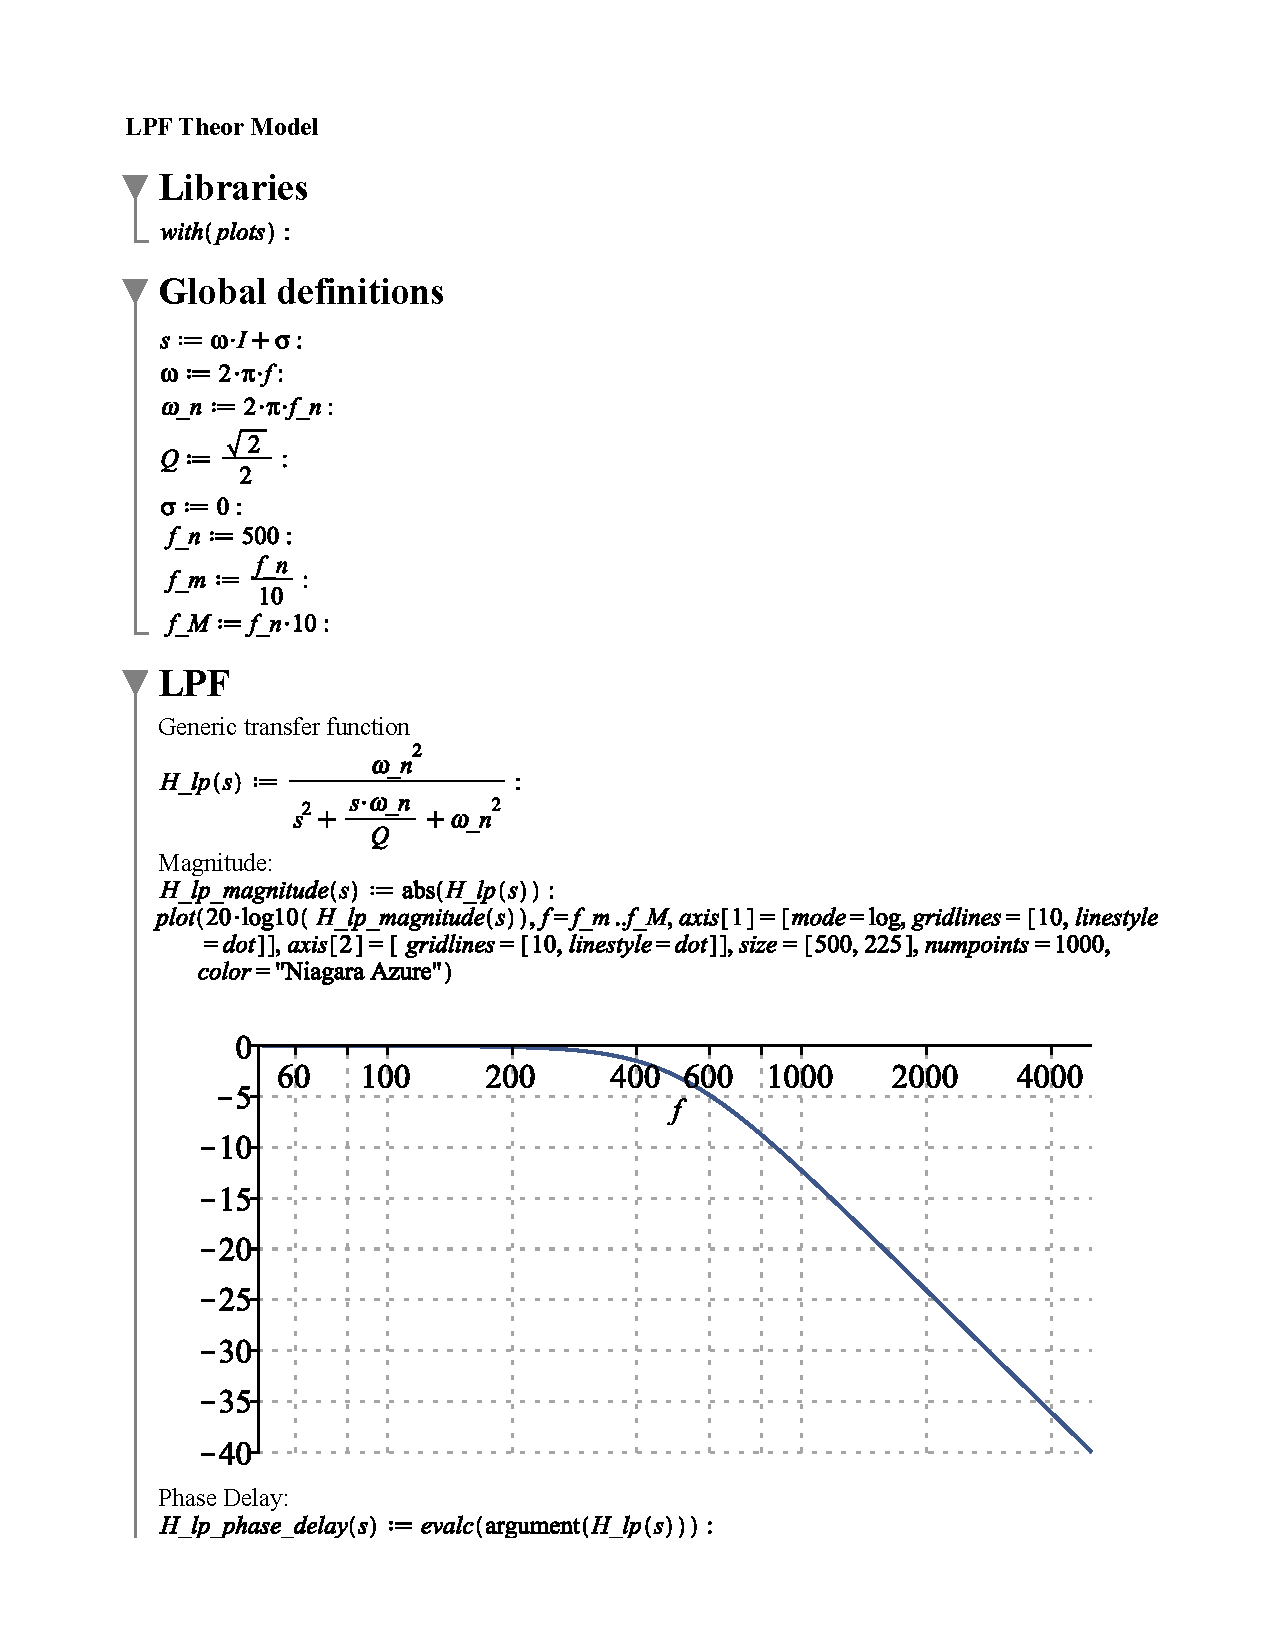
\includepdf[pages=-]{media/maple/lpf_theor-model.pdf}
    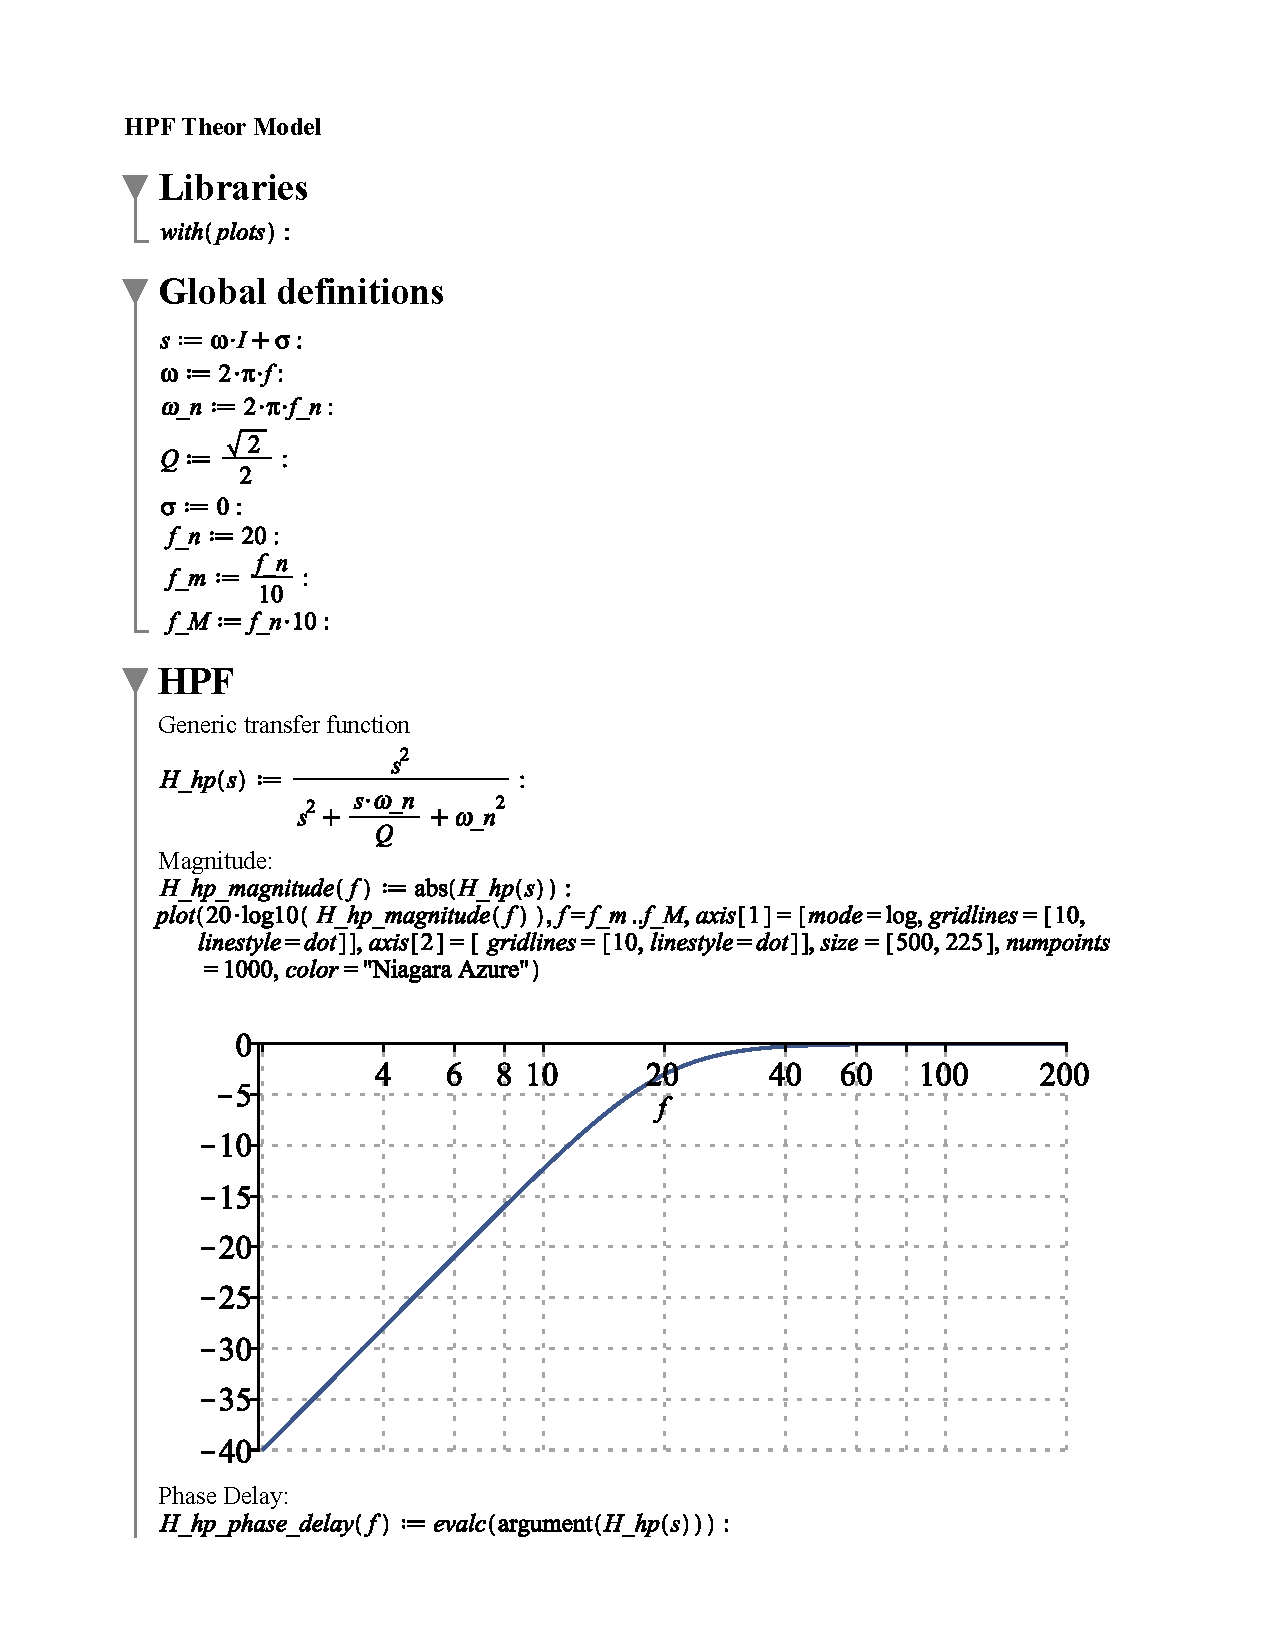
\includepdf[pages=-]{media/maple/hpf_theor-model.pdf}
    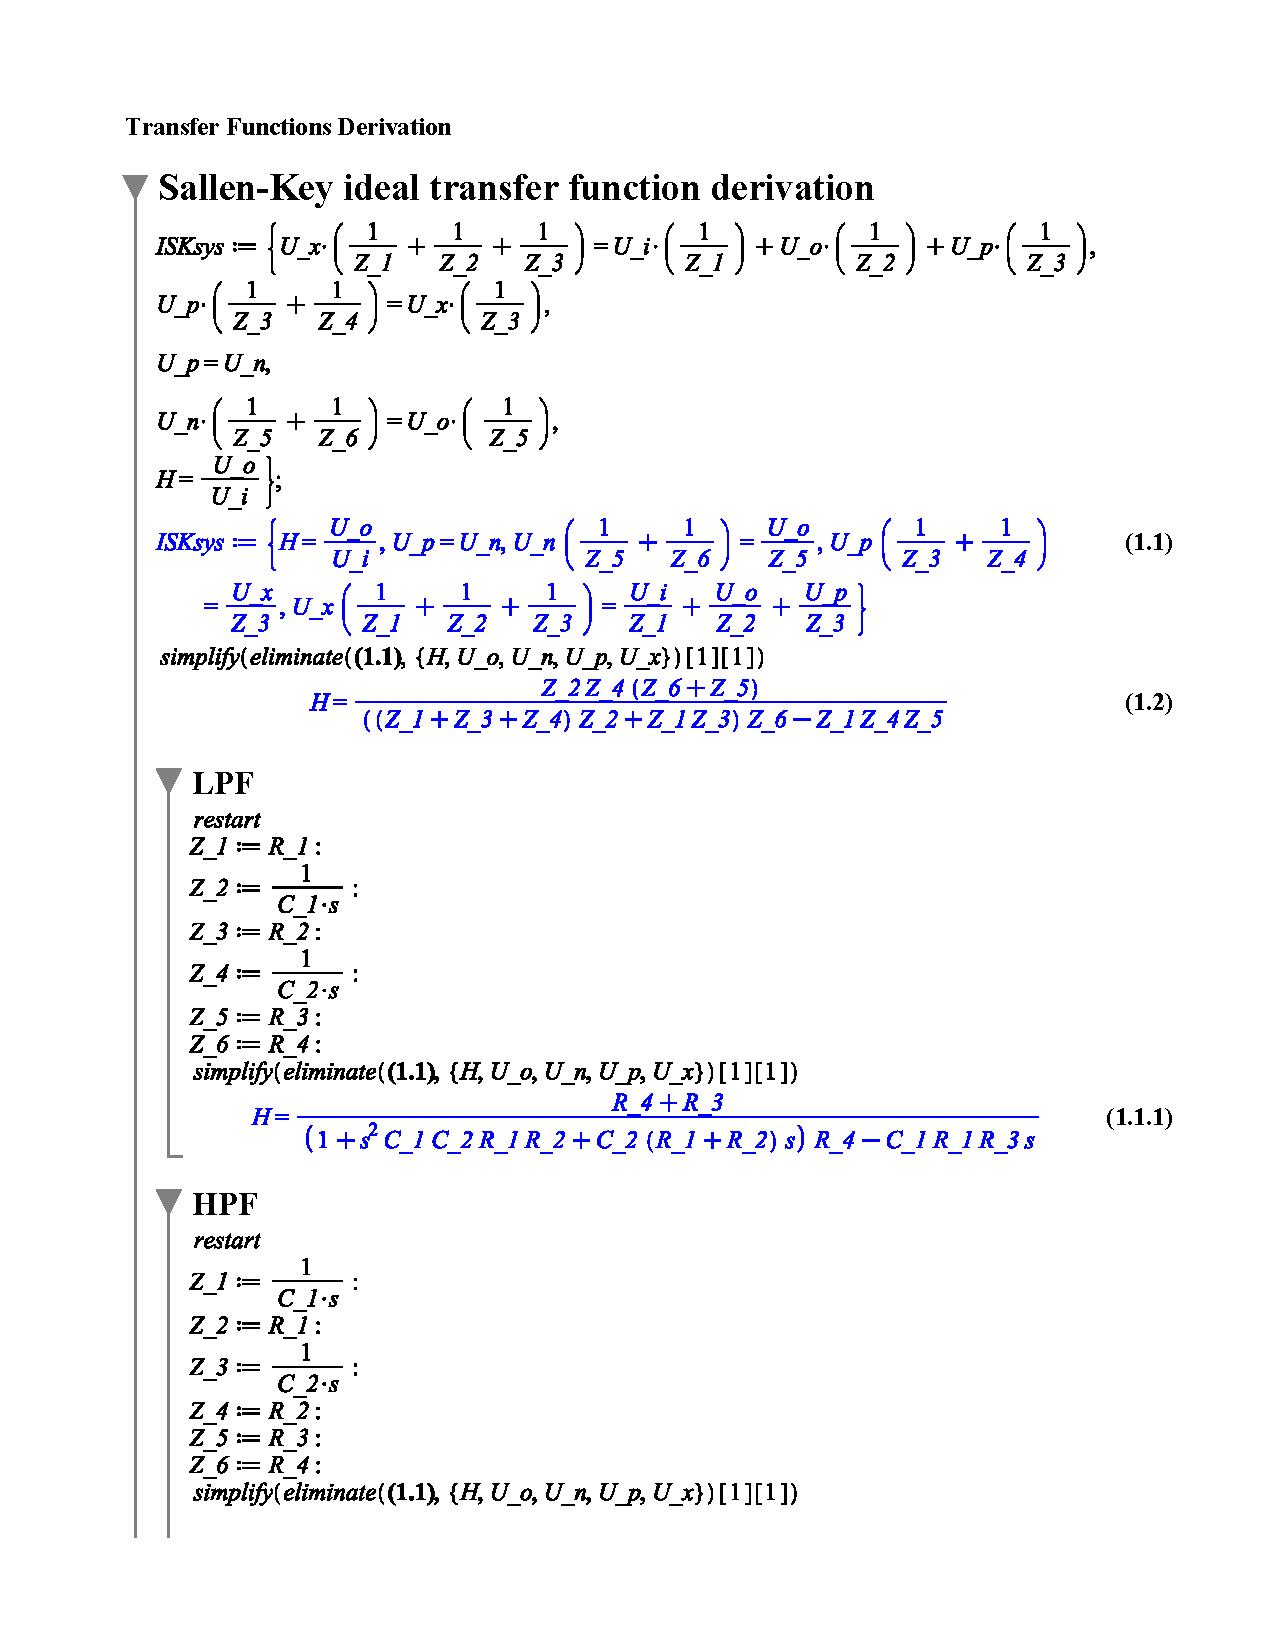
\includepdf[pages=-]{media/maple/tranfer_functions_derivation.pdf}
    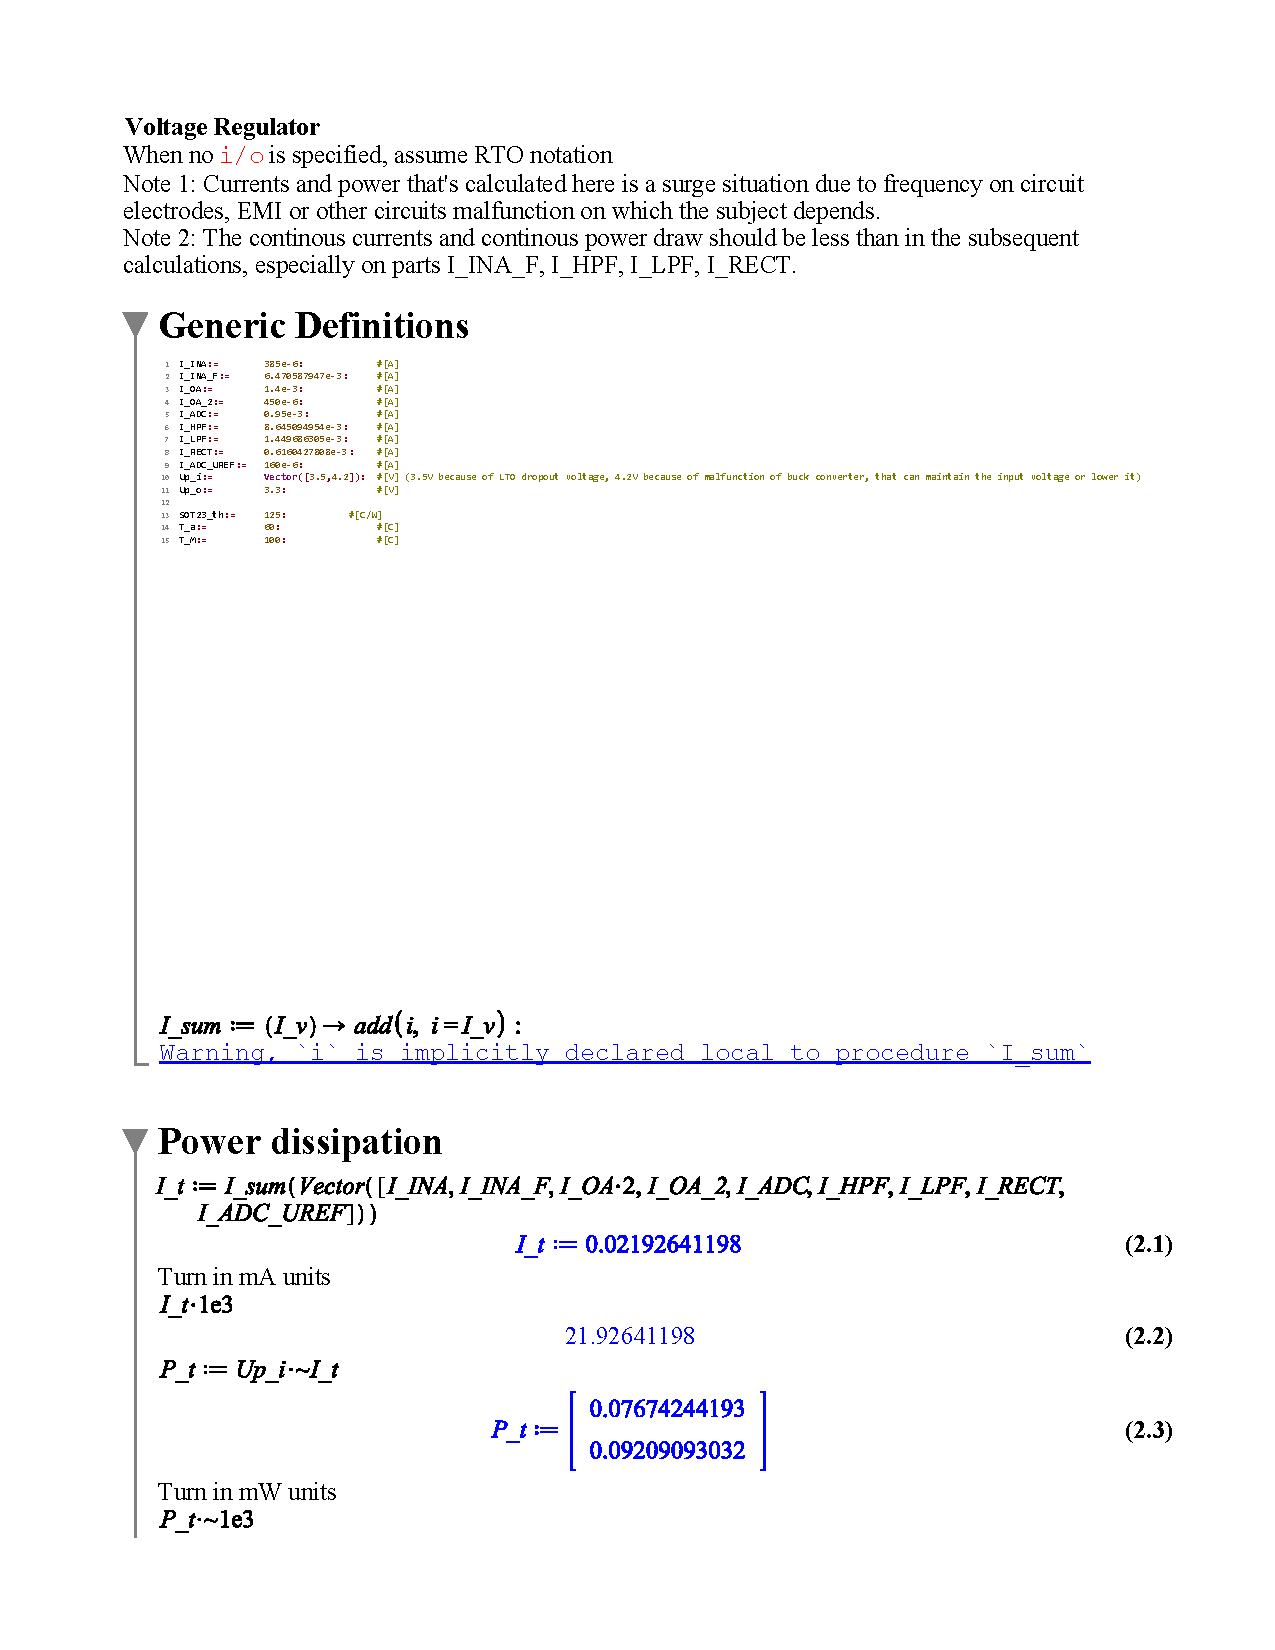
\includepdf[pages=-]{media/maple/voltage_regulator.pdf}
    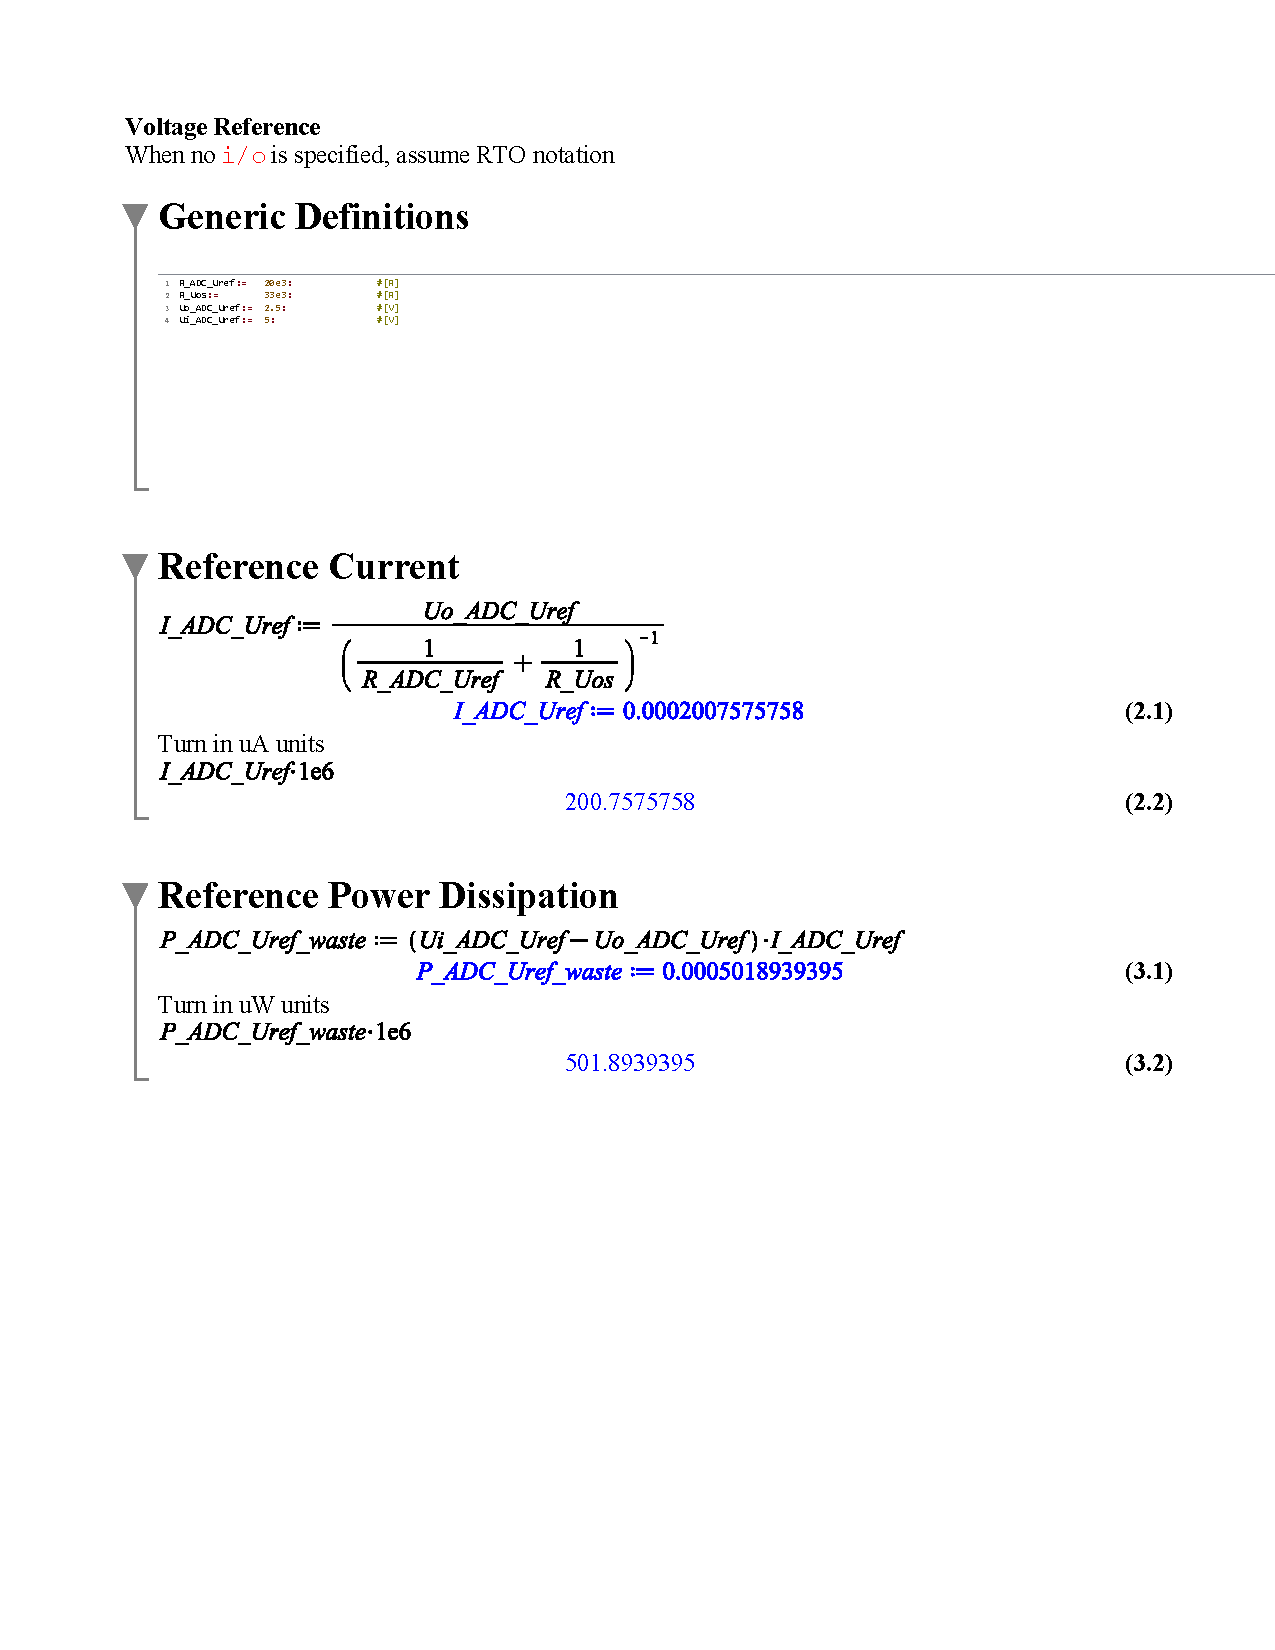
\includepdf[pages=-]{media/maple/voltage_reference.pdf}
    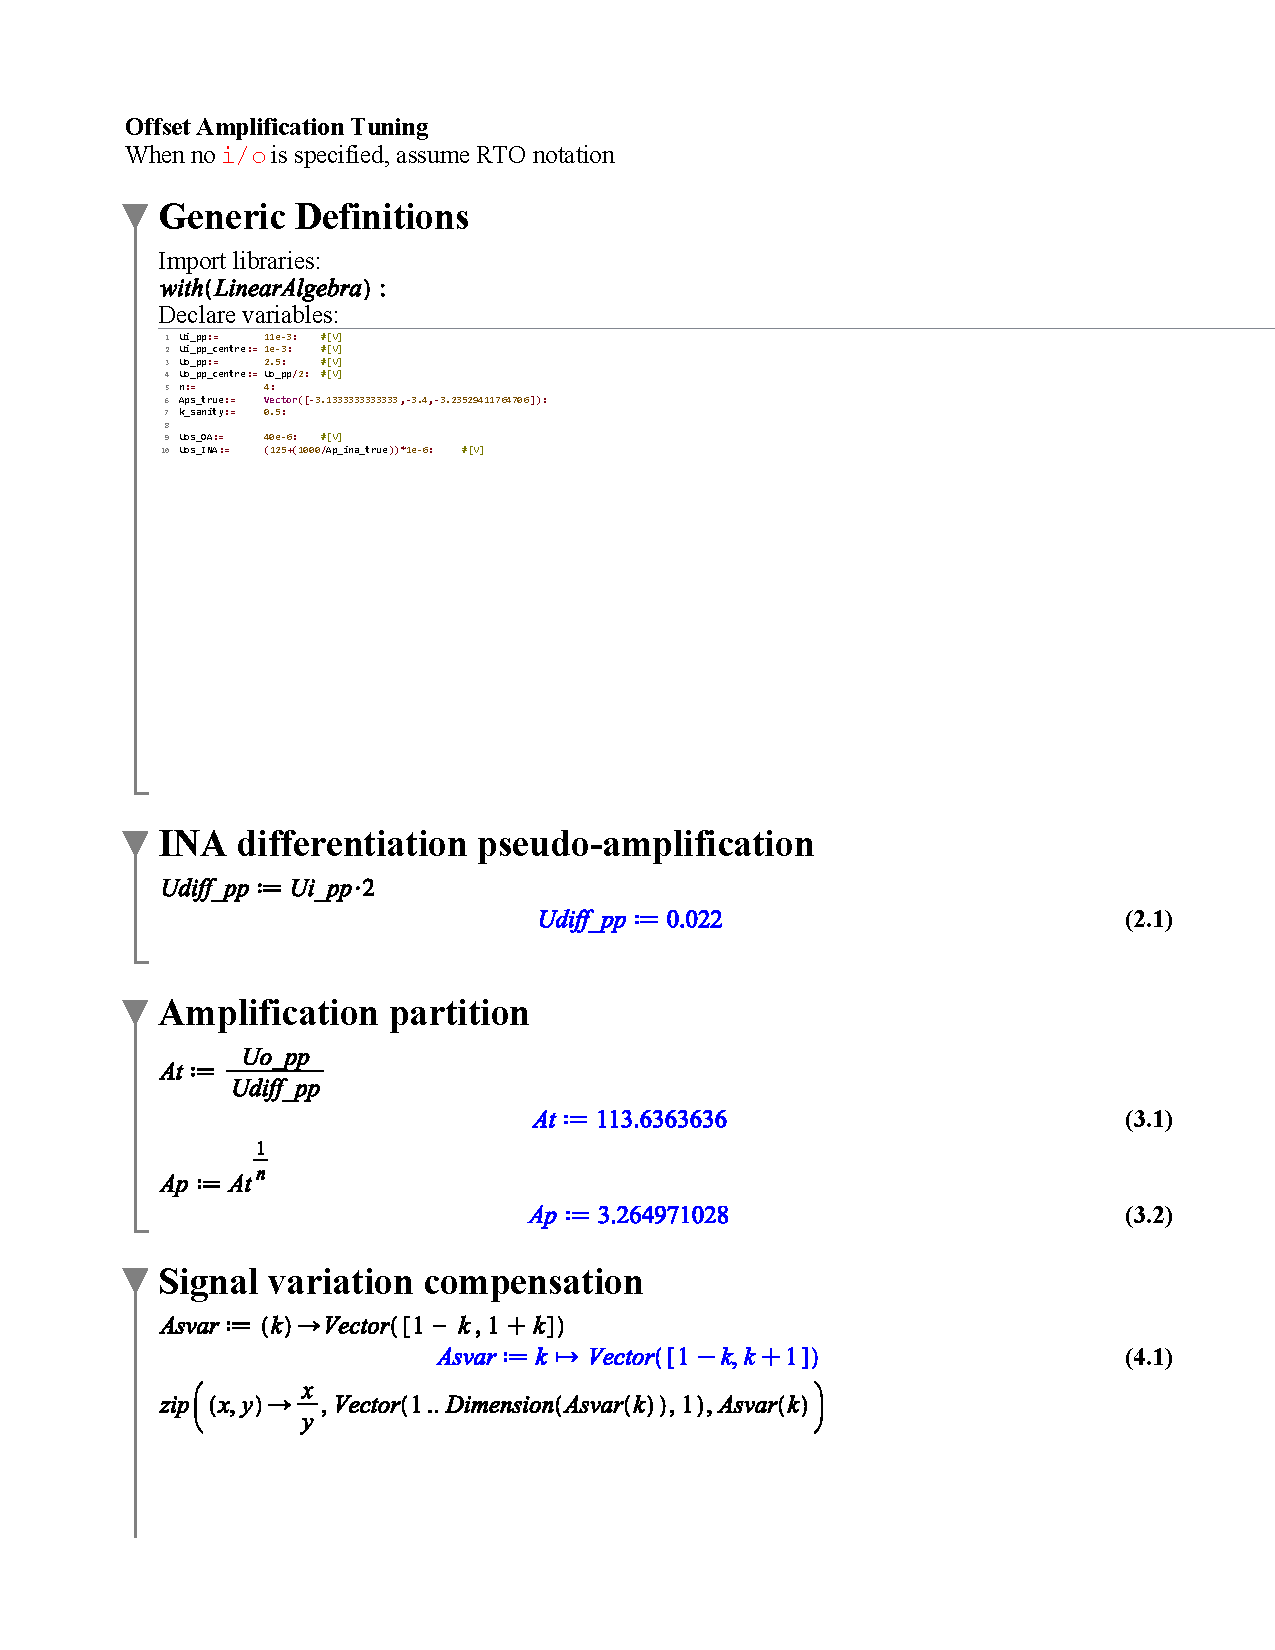
\includepdf[pages=-]{media/maple/offset_amplification_tuning.pdf}
    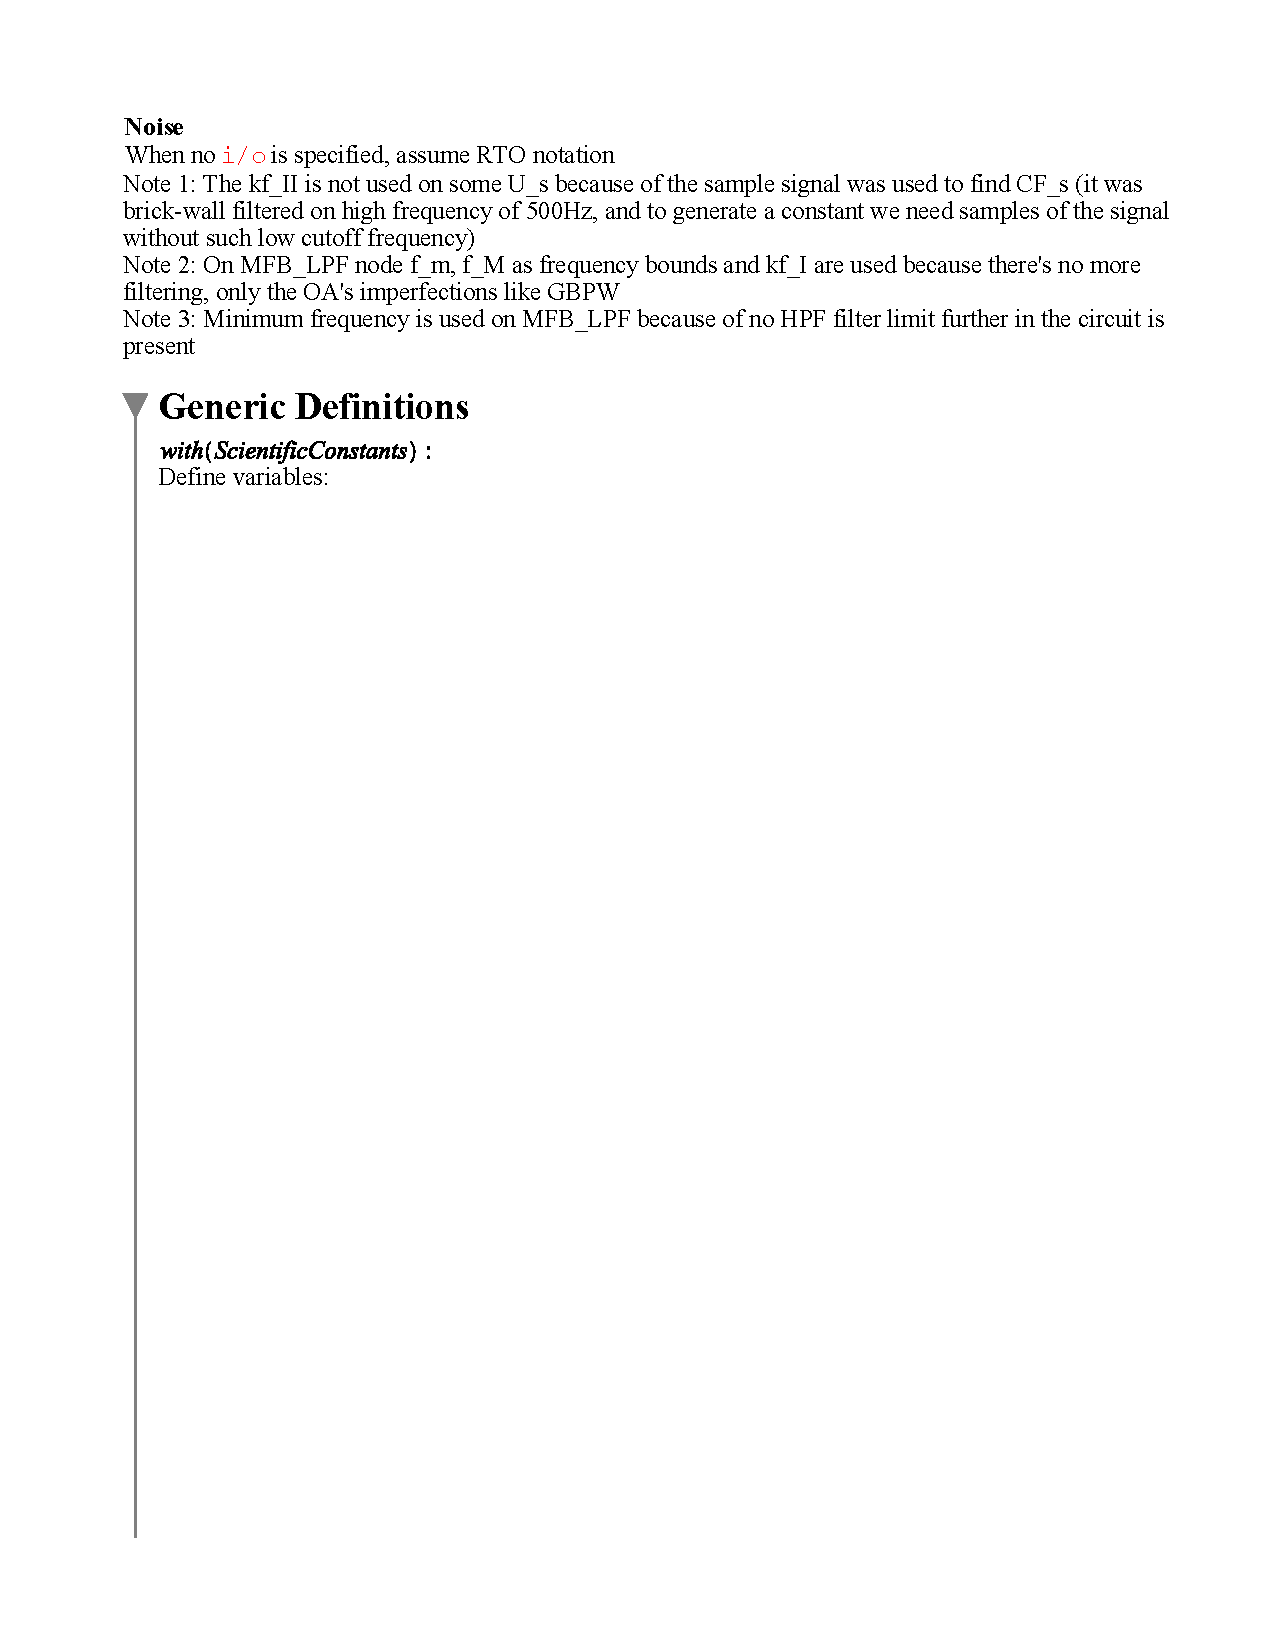
\includepdf[pages=-]{media/maple/noise.pdf}
    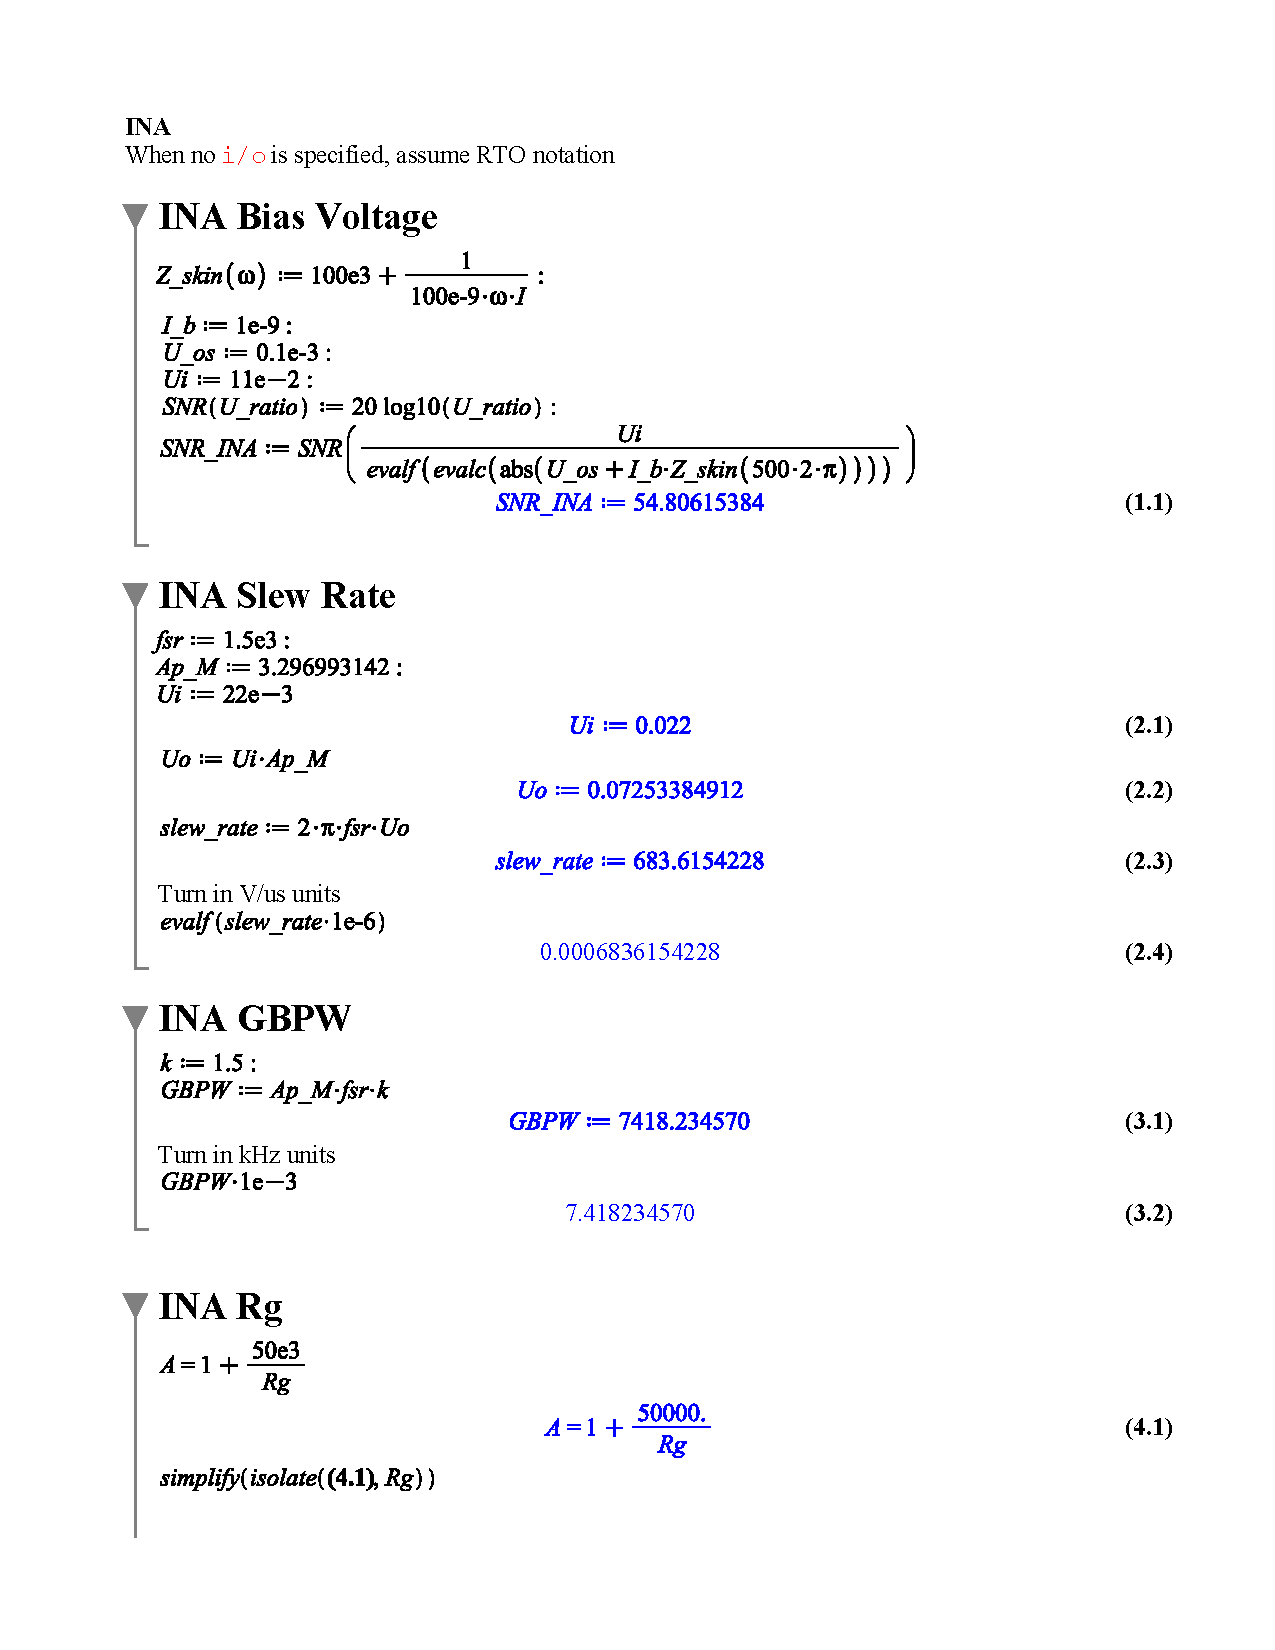
\includepdf[pages=-]{media/maple/INA.pdf}
    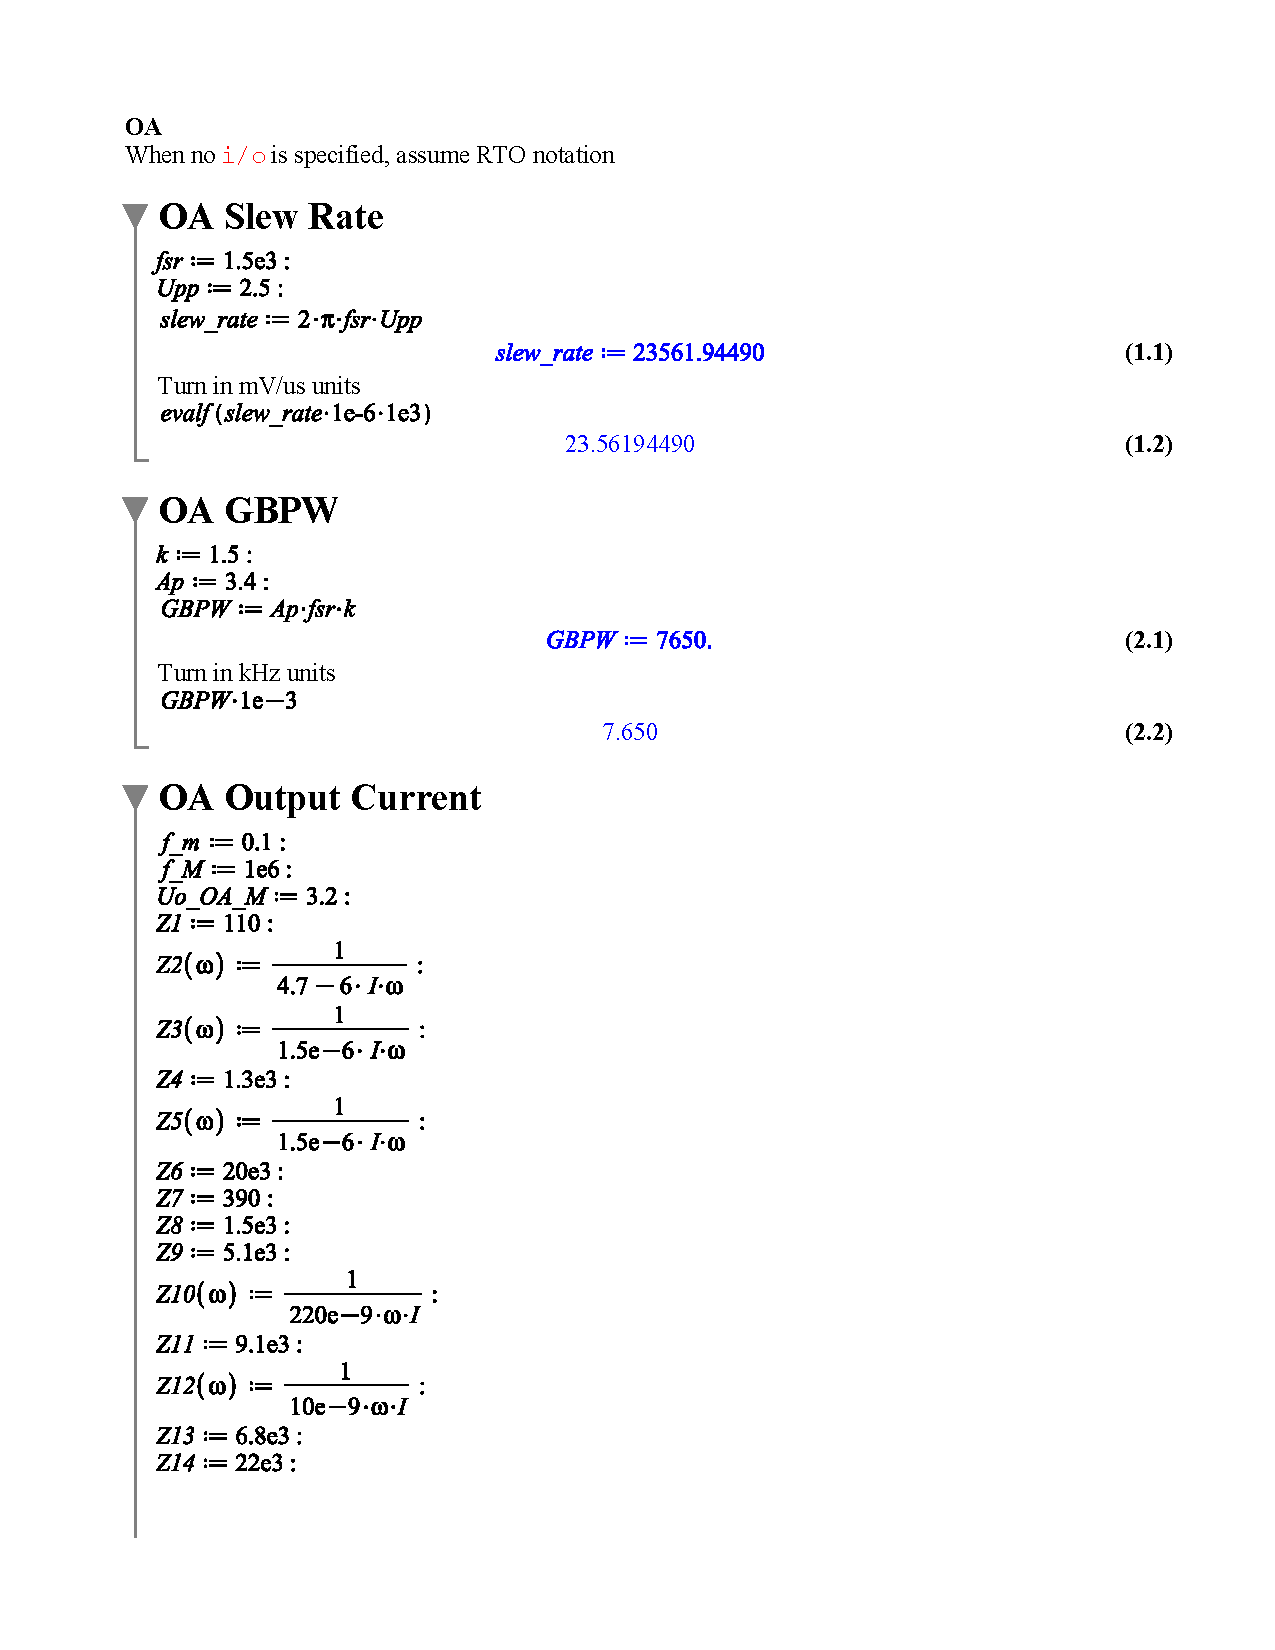
\includepdf[pages=-]{media/maple/OA.pdf}
    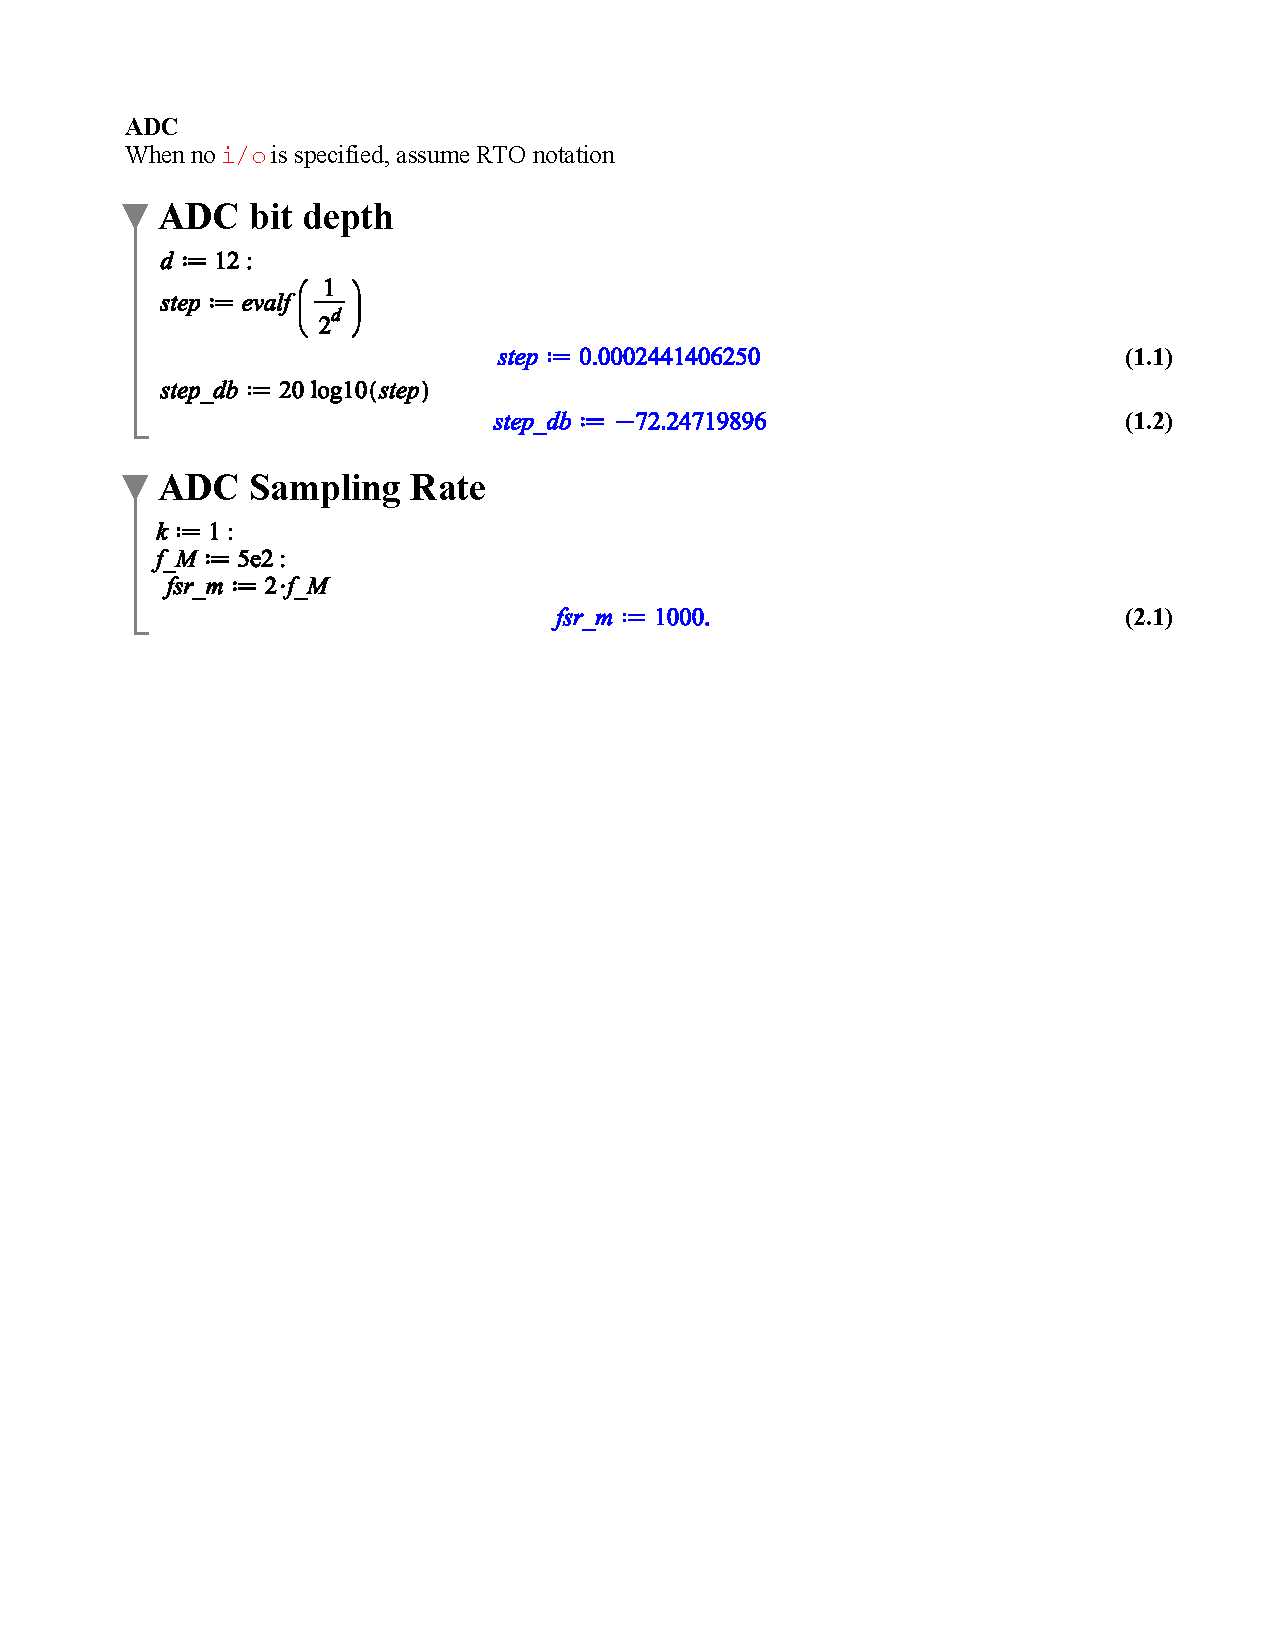
\includepdf[pages=-]{media/maple/ADC.pdf}

    \printbibheading
    \printbibliography[keyword=major, heading=subbibliography, title={Основные источники}]
    \printbibliography[keyword=minor, heading=subbibliography, title={Второстепенные источники}]
    \printbibliography[keyword=data, heading=subbibliography, title={Источники данных}]
    \printbibliography[keyword=image, heading=subbibliography, title={Источники изображений}]
    \printbibliography[keyword=datasheet, heading=subbibliography, title={Техническая документация}]
    \printbibliography[keyword=software, heading=subbibliography, title={Программное обеспечение}]
    % TRANSLATOR NOTE: "Sorgenti Software" / "Sorgenti Componenti" have no given mapping; translated as "Программное обеспечение" / "Источники компонентов".
    \printbibliography[keyword=web, heading=subbibliography, title={Источники компонентов}]
\end{document}
